\documentclass[a4paper, 12pt, twoside, openright, bibliography=totoc, USenglish,
	final % replace with final for handing in
]{scrbook}
\setcounter{secnumdepth}{5}

% https://tex.stackexchange.com/questions/108684/spacing-before-and-after-section-titles
% https://tex.stackexchange.com/questions/48753/obtaining-the-default-section-spacing-into-the-titlespacing-parameters
\usepackage{titlesec}

% https://tex.stackexchange.com/questions/299969/titlesec-loss-of-section-numbering-with-the-new-update-2016-03-15
\usepackage{etoolbox}
\makeatletter
\patchcmd{\ttlh@hang}{\parindent\z@}{\parindent\z@\leavevmode}{}{}
\patchcmd{\ttlh@hang}{\noindent}{}{}{}
\makeatother

\titleformat{\chapter}[display]
{\sffamily \huge \bfseries}{\chaptertitlename\ \thechapter}{20pt}{\Huge}
\titleformat{\section}[hang]
{\sffamily \Large \bfseries}{\thesection}{1em}{}
\titleformat{\subsection}[hang]
{\sffamily \large \bfseries}{\thesubsection}{1em}{}
\titleformat{\subsubsection}[hang]
{\sffamily \normalsize \bfseries}{\thesubsubsection}{1em}{}
\titleformat{\paragraph}[runin]
{\sffamily \normalsize \bfseries}{\theparagraph}{1em}{}
\titleformat{\subparagraph}[runin]
{\sffamily \normalsize \bfseries}{\thesubparagraph}{1em}{}

\titlespacing*{\chapter} {0pt}{45pt}{35pt}
\titlespacing*{\section} {0pt}{2.5ex plus 0.5ex minus 0.25ex}{2.25ex plus 0.25ex}
\titlespacing*{\subsection} {0pt}{2.25ex plus 0.5ex minus 0.25ex}{1.5ex plus 0.25ex}
\titlespacing*{\subsubsection}{0pt}{2.25ex plus 0.5ex minus 0.25ex}{1.5ex plus 0.25ex}
\titlespacing*{\paragraph} {0pt}{2.25ex plus 0.5ex minus 0.25ex}{1em}
\titlespacing*{\subparagraph} {\parindent}{2.25ex plus 0.5ex minus 0.25ex}{1em}

% chapter heading style
\usepackage{fncychap}
\ChNameVar{\sffamily \huge \bfseries}
\ChTitleVar{\sffamily \huge \bfseries}
%\declaretheoremstyle[headfont=\ttfamily]{normalhead}

% variables
\usepackage{titling}
\makeatletter
\newcommand{\thesis}{master} % possible values: bachelor, master
\newbool{uselogo}
\booltrue{uselogo} % remove this line if you do NOT want to use the logo (you have to sign the form when you use it)
\title{Learning Shape Completion from Bounding Boxes with CAD Shape Priors}
\author{David Stutz}
\date{13.09.2017}
\newcommand{\erstgutachter}{Prof. Dr. Bastian Leibe}
\newcommand{\zweitgutachter}{Prof. Dr. Andreas Geiger}
% Max Planck Institute for Intelligent Systems, Autonomous Vision Group and ETH Z\"{u}rich, Computer Vision and Geometry Group
\makeatother

\newcommand{\specialcell}[2][c]{%
  \begin{tabular}[#1]{@{}c@{}}#2\end{tabular}}
  
% language
\usepackage[USenglish,ngerman]{babel}
\usepackage[utf8]{inputenc}
\usepackage[iso]{isodate}

% colors
\usepackage[table]{xcolor}

% citations
\usepackage{cite}

%page geometry (for nicer margins on the title page)
\usepackage[a4paper, twoside, inner=3.5cm, outer=3cm, bottom=4cm]{geometry}
\usepackage{scrextend}
\usepackage[final]{graphicx}
\graphicspath{{./images/}}
\usepackage{wrapfig}
\usepackage{float}
\usepackage{tabularx}
\usepackage[bf,font=footnotesize]{caption}
\DeclareCaptionFont{better}{\normalfont\bfseries\sffamily}
% https://tex.stackexchange.com/questions/57117/algorithms-package-ignores-caption-package
\captionsetup[algorithm]{font=footnotesize}
\captionsetup{labelfont=better}

% https://tex.stackexchange.com/questions/32614/vertical-spacing-in-floats
\setlength{\belowcaptionskip}{-\baselineskip}\addtolength{\belowcaptionskip}{1ex}

% https://tex.stackexchange.com/questions/19766/how-to-control-the-position-of-floating-images
\usepackage{placeins}

\captionsetup{format=plain}
\usepackage[font=footnotesize]{subcaption}
\addtolength{\abovecaptionskip}{-2mm}
\renewcommand{\topfraction}{0.9}
\renewcommand{\bottomfraction}{0.8}
\setcounter{topnumber}{2}
\setcounter{bottomnumber}{2}
\setcounter{totalnumber}{4}
\setcounter{dbltopnumber}{2}
\renewcommand{\dbltopfraction}{0.9}
\renewcommand{\textfraction}{0.07}
\renewcommand{\floatpagefraction}{0.95}
\renewcommand{\dblfloatpagefraction}{0.95}

% https://tex.stackexchange.com/questions/28627/how-to-install-the-algorithms-package
\usepackage[section]{algorithm}
%\captionsetup[algorithm]{font=footnotesize}
\usepackage[numbered]{algo}

\usepackage{sidecap}
\usepackage{pgfplots}
\usepackage{tikz}
\usetikzlibrary{positioning}
\usetikzlibrary{decorations.pathreplacing}
\usetikzlibrary{backgrounds}
\usetikzlibrary{shapes.misc}
% https://tex.stackexchange.com/questions/164991/pgfplots-how-to-fill-bounded-area-under-a-curve-using-addplot-and-fill
\usepgfplotslibrary{fillbetween}

\pgfplotsset{
  label style={font=\scriptsize},
  tick label style={font=\scriptsize},
  legend style={font=\scriptsize},
}

% https://tex.stackexchange.com/questions/13627/pgfplots-multiple-shifted-stacked-plots-in-one-diagram
\makeatletter
\newcommand\resettenstackedplots{
\makeatletter
\pgfplots@stacked@isfirstplottrue
\makeatother
\addplot [forget plot,draw=none] coordinates{
  (1,0) (2,0) (3,0) (4, 0) (5, 0)
  (6,0) (7,0) (8,0) (9, 0) (10, 0)
};
}
\makeatother
\makeatletter
\newcommand\resetelevenstackedplots{
\makeatletter
\pgfplots@stacked@isfirstplottrue
\makeatother
\addplot [forget plot,draw=none] coordinates{
  (1,0) (2,0) (3,0) (4, 0) (5, 0)
  (6,0) (7,0) (8,0) (9, 0) (10, 0)
  (11, 0)
};
}
\makeatother
\makeatletter
\newcommand\resettwelvestackedplots{
\makeatletter
\pgfplots@stacked@isfirstplottrue
\makeatother
\addplot [forget plot,draw=none] coordinates{
  (1,0) (2,0) (3,0) (4, 0) (5, 0)
  (6,0) (7,0) (8,0) (9, 0) (10, 0)
  (11, 0) (12, 0)
};
}
\makeatother

% https://tex.stackexchange.com/questions/11368/bell-curve-gaussian-function-normal-distribution-in-tikz-pgf
\makeatletter
\pgfmathdeclarefunction{gauss}{2}{%
  \pgfmathparse{1/(#2*sqrt(2*pi))*exp(-((x-#1)^2)/(2*#2^2))}%
}
\makeatother

% https://tex.stackexchange.com/questions/107423/erf-function-in-latex
\makeatletter
\pgfmathdeclarefunction{erf}{1}{%
  \begingroup
    \pgfmathparse{#1 > 0 ? 1 : -1}%
    \edef\sign{\pgfmathresult}%
    \pgfmathparse{abs(#1)}%
    \edef\x{\pgfmathresult}%
    \pgfmathparse{1/(1+0.3275911*\x)}%
    \edef\t{\pgfmathresult}%
    \pgfmathparse{%
      1 - (((((1.061405429*\t -1.453152027)*\t) + 1.421413741)*\t 
      -0.284496736)*\t + 0.254829592)*\t*exp(-(\x*\x))}%
    \edef\y{\pgfmathresult}%
    \pgfmathparse{(\sign)*\y}%
    \pgfmath@smuggleone\pgfmathresult%
  \endgroup
}
\makeatother

\usepackage{xcolor}
\definecolor{fc}{HTML}{1E90FF}
\definecolor{h}{HTML}{228B22}
\definecolor{bias}{HTML}{87CEFA}
\definecolor{noise}{HTML}{8B008B}
\definecolor{conv}{HTML}{FFA500}
\definecolor{pool}{HTML}{B22222}
\definecolor{up}{HTML}{B22222}
\definecolor{view}{HTML}{FFFFFF}
\definecolor{bn}{HTML}{FFD700}
\tikzset{fc/.style={black,draw=black,fill=fc,rectangle,minimum height=1cm}}
\tikzset{h/.style={black,draw=black,fill=h,rectangle,minimum height=1cm}}
\tikzset{bias/.style={black,draw=black,fill=bias,rectangle,minimum height=1cm}}
\tikzset{noise/.style={black,draw=black,fill=noise,rectangle,minimum height=1cm}}
\tikzset{conv/.style={black,draw=black,fill=conv,rectangle,minimum height=1cm}}
\tikzset{pool/.style={black,draw=black,fill=pool,rectangle,minimum height=1cm}}
\tikzset{up/.style={black,draw=black,fill=up,rectangle,minimum height=1cm}}
\tikzset{view/.style={black,draw=black,fill=view,rectangle,minimum height=1cm}}
\tikzset{bn/.style={black,draw=black,fill=bn,rectangle,minimum height=1cm}}

\usepackage[sumlimits, intlimits]{amsmath}

% https://tex.stackexchange.com/questions/69662/how-to-globally-change-the-spacing-around-equations
\makeatletter
\g@addto@macro\normalsize{%
  \setlength\abovedisplayskip{6pt}
  \setlength\belowdisplayskip{6pt}
  \setlength\abovedisplayshortskip{6pt}
  \setlength\belowdisplayshortskip{6pt}
}

%\usepackage{amsthm}
\usepackage{amssymb}
\usepackage{amsfonts}
% https://tex.stackexchange.com/questions/26637/how-do-you-get-mathbb1-to-work-characteristic-function-of-a-set
\usepackage{dsfont}

%\theoremstyle{definition}
%\newtheorem{definition}{Definition}[section]
%\theoremstyle{theorem}
%\newtheorem*{theorem}{Theorem}
%\theoremstyle{lemma}
%\newtheorem*{lemma}{Lemma}
%\theoremstyle{example}
%\newtheorem*{example}{Example}
%\theoremstyle{problem}
%\newtheorem*{problem}{Problem}

% https://packages.ubuntu.com/trusty/texlive-fonts-extra
\usepackage{mathabx}
\usepackage{thmtools}
\usepackage[thmmarks]{ntheorem}
\theoremheaderfont{\normalfont\bfseries\sffamily}
\theorempreskip{6px}
\theorempostskip{6px}
\newtheorem{example}{Example}[chapter]
\newtheorem{problem}{Problem}[chapter]
\newtheorem{definition}{Definition}[chapter]
\newtheorem{remark}{Remark}[chapter]
\newtheorem{theorem}{Theorem}[chapter]
\newtheorem{lemma}{Lemma}[chapter]
\newtheorem{corollary}{Corollary}[chapter]

\theoremstyle{nonumberplain}
\theoremheaderfont{\itshape}
\theorembodyfont{\normalfont}
%\theoremseparator{.\,—}
\theoremsymbol{}
\newtheorem{proof-wo}{Proof}
\theoremsymbol{\ensuremath{\color{lightgray}\blacksquare}}
\newtheorem{proof}{Proof: }

\usepackage[final]{listings}

% https://tex.stackexchange.com/questions/161549/scaling-inline-code-to-the-current-font-size
\makeatletter
\lstdefinestyle{mystyle}{
  basicstyle=%
    \ttfamily
    %\color{blue}%
    \lst@ifdisplaystyle\scriptsize\fi
}
\makeatother
\lstset{style=mystyle}

\usepackage[toc,page]{appendix}
\usepackage{enumerate}
\usepackage[subfigure]{tocloft}
\usepackage{multirow}
\newcommand{\mycirc}[1][black]{\begin{Large}
\textcolor{#1}{\ensuremath\bullet}
\end{Large}}

% hyperref
\usepackage[final]{hyperref}
\hypersetup{
	pdfauthor={\theauthor},
	pdftitle={\thetitle},
	colorlinks,
	linkcolor=black,
	citecolor=black,
	a4paper=true,
	plainpages=false,
	breaklinks=true,
}

% headers and footers
\usepackage{afterpage}
\usepackage{fancyhdr}
\fancyhf{}
\fancyhead[RO, LE]{\nouppercase{\leftmark}}
\fancyhead[RE, LO]{\nouppercase{\rightmark}}
\fancyfoot[RO, LE]{\thepage}
\fancypagestyle{fancytitle}{
	\fancyhf{}
	\begin{tikzpicture}[overlay, remember picture]
		\node[anchor=north east, xshift=-1mm, yshift=-1.5mm] at (current page.north east){\includegraphics[width=0.54\paperwidth]{./logo/logo.pdf}};
		\node[anchor=north west, xshift=1mm, yshift=-1.5mm] at (current page.north west){
\includegraphics[width=0.34\paperwidth]{./logo/mpi_is}};
	\end{tikzpicture}
	
	\renewcommand{\headrulewidth}{0pt}
	\setlength{\headheight}{60pt}
}
\fancypagestyle{plain}{
	\fancyhf{}
	%\fancyhead{}
	\fancyfoot[R]{\thepage}%
	\renewcommand{\headrulewidth}{0pt}
}
\fancypagestyle{number}{
	\fancyhf{}
	\fancyhead{}
	\fancyfoot[R]{\thepage}%
	\renewcommand{\headrulewidth}{0pt}
}
\fancypagestyle{empty}{
	\fancyhf{}
	\fancyhead{}
	%\fancyfoot{}
	\renewcommand{\headrulewidth}{0pt}
}

\newcommand{\clearemptydoublepage}{\newpage{\pagestyle{empty}\cleardoublepage}}

% latex optimization parameters
\clubpenalty = 10000
\widowpenalty = 10000
\displaywidowpenalty = 10000

\usepackage{mathtools}
\mathtoolsset{showonlyrefs}
\DeclarePairedDelimiter\ceil{\lceil}{\rceil}
\DeclarePairedDelimiter\floor{\lfloor}{\rfloor}

% math
\newcommand{\Cin}{\ensuremath{C_{\text{in}}}}
\newcommand{\Cout}{\ensuremath{C_{\text{out}}}}
\newcommand{\cin}{\ensuremath{c_{\text{in}}}}
\newcommand{\cout}{\ensuremath{c_{\text{out}}}}
\newcommand{\Ber}{\ensuremath{\mathrm{Ber}}}
\newcommand{\Gu}{\ensuremath{\mathrm{Gu}}}
\newcommand{\Dis}{\ensuremath{\mathrm{Dis}}}
\newcommand{\const}{\ensuremath{\mathrm{const}}}
\newcommand{\Var}{\ensuremath{\mathrm{Var}}}
\newcommand{\Cov}{\ensuremath{\mathrm{Cov}}}
\newcommand{\Tr}{\ensuremath{\mathrm{Tr}}}
\newcommand{\diag}{\ensuremath{\mathrm{diag}}}
\newcommand{\erf}{\ensuremath{\mathrm{erf}}}
\newcommand{\Vol}{\ensuremath{\mathrm{Vol}}}
\newcommand{\Exp}{\ensuremath{\mathrm{Exp}}}
\newcommand{\KL}{\ensuremath{\mathrm{KL}}}
\newcommand{\uk}{\ensuremath{\bot}}
\DeclareMathOperator*{\argmin}{argmin}
\DeclareMathOperator*{\argmax}{argmax}
% https://tex.stackexchange.com/questions/214904/what-is-the-latex-convention-for-sign-function
\DeclareMathOperator{\sign}{sign}
\DeclareMathOperator{\ReLU}{ReLU}

% abbreviations
\usepackage{xspace}
\newcommand*{\eg}{\emph{e.g.}\@\xspace}
\newcommand*{\Eg}{\emph{E.g.}\@\xspace}
\newcommand*{\ie}{\emph{i.e.}\@\xspace}
\newcommand*{\etc}{\emph{etc.}\@\xspace}
\newcommand*{\etal}{\emph{et al.}\@\xspace}
\newcommand*{\cf}{\emph{cf.}\@\xspace}
\newcommand*{\vs}{\emph{vs.}\@\xspace}

\newcommand*{\Rect}{\lstinline!2D!\@\xspace}
\newcommand*{\Cub}{\lstinline!3D!\@\xspace}
\newcommand*{\ShapeNet}{\lstinline!ShapeNet!\@\xspace}

\newcommand*{\hard}{\lstinline!hard!\@\xspace}
\newcommand*{\moderate}{\lstinline!moderate!\@\xspace}
\newcommand*{\easy}{\lstinline!easy!\@\xspace}

\newcommand*{\PPCA}{\lstinline!PPCA!\@\xspace}
\newcommand*{\VAE}{\lstinline!VAE!\@\xspace}
\newcommand*{\DVAE}{\lstinline!DVAE!\@\xspace}
\newcommand*{\VAEs}{\lstinline!VAEs!\@\xspace}
\newcommand*{\DVAEs}{\lstinline!DVAEs!\@\xspace}
\newcommand*{\ML}{\lstinline!ML!\@\xspace}
\newcommand*{\DL}{\lstinline!DL!\@\xspace}
\newcommand*{\AML}{\lstinline!AML!\@\xspace}
\newcommand*{\EVAE}{\lstinline!EVAE!\@\xspace}
\newcommand*{\EVAEs}{\lstinline!EVAEs!\@\xspace}

\def\NLL{\text{NLL}\xspace}
\def\Abs{\text{Abs}\xspace}
\DeclareRobustCommand{\AbsThr}{%
    \ifmmode
        \text{Abs}_{\text{thresh}}
    \else
        $\text{Abs}_{\text{thresh}}$
    \fi
}

% http://tex.stackexchange.com/questions/3033/forcing-linebreaks-in-url
\usepackage{url}
\expandafter\def\expandafter\UrlBreaks\expandafter{\UrlBreaks%  save the current one
\do\a\do\b\do\c\do\d\do\e\do\f\do\g\do\h\do\i\do\j%
\do\k\do\l\do\m\do\n\do\o\do\p\do\q\do\r\do\s\do\t%
\do\u\do\v\do\w\do\x\do\y\do\z\do\A\do\B\do\C\do\D%
\do\E\do\F\do\G\do\H\do\I\do\J\do\K\do\L\do\M\do\N%
\do\O\do\P\do\Q\do\R\do\S\do\T\do\U\do\V\do\W\do\X%
\do\Y\do\Z}

\RequirePackage{snapshot}
\begin{document}
  \selectlanguage{USenglish}
  \pagestyle{fancy}

  % titlepage
  \frontmatter
  \begin{titlepage}
  \thispagestyle{fancytitle}
  \newgeometry{left=2cm,right=7mm}
  \begin{center}

  {
    Diese Arbeit wurde vorgelegt am\\
    Lehr- und Forschungsgebiet Informatik 8 (Computer Vision)\\
    Fakultät für Mathematik, Informatik und Naturwissenschaften\\
    Prof. Dr. Bastian Leibe
  }

  \vspace{1em}

  % headrule
  \rule{\linewidth}{0.5mm}
  ~\\[2em]

  {
    \huge \bfseries\sffamily
    \ifthenelse{\equal{\thesis}{master}}{Master}{Bachelor} Thesis
  }

  \vfill

  \begin{addmargin}[1em]{1em}
    \centering
    \sffamily \huge \bfseries \thetitle
  \end{addmargin}

  \vfill

  {
    vorgelegt von
			
    \textsf{\textbf{\theauthor}}\\
    \thedate
  }

  % bottomrule
  ~\\[2em]
  \rule{\linewidth}{0.5mm}

  \vspace{2em}

  \begin{tabular}{ll}
    Erstgutachter:  & \erstgutachter\\
    Zweitgutachter: & \zweitgutachter\\
  \end{tabular}
	
  \end{center}
  \restoregeometry
\end{titlepage}


  \clearemptydoublepage
  
  \thispagestyle{number}
  \tableofcontents
  %\listoffigures
  \clearemptydoublepage

  % main content
  \mainmatter
  
  \chapter{Introduction}

% Human Perception of 3D Shapes https://link.springer.com/chapter/10.1007/978-3-540-74272-2_1
Shape perception is a long-standing and fundamental problem both in human
\cite{Pizlo:2007,Pizlo:2010}
and computer vision \cite{FurukawaHernandez:2015}.
In both disciplines, a large body of work focuses on 3D reconstruction, \eg
reconstructing objects or scenes from one or more views. 
The problem of reconstructing 3D scenes or objects is an inherently ill-posed
inverse problem because many configurations of shape, color, texture and
lighting may give rise to the very same views \cite{FurukawaHernandez:2015}.
In human vision, one of the fundamental problems is understanding
how the human visual system accomplishes such tasks; in computer vision,
in contrast, the goal is to develop 3D reconstruction systems.
Both disciplines are related through insights regarding the cues and constraints
used by humans to perceive 3D shapes. Results from human vision \cite{Pizlo:2007,Pizlo:2010}
suggest that these priors as well as the ability to process the provided cues
is innate and not learned. In computer vision, as well, cues and priors are commonly
built into 3D reconstruction pipelines through explicit assumptions.
Recently, however -- leveraging the success of deep learning -- researchers
started to learn shape models from data. Predominantly generative models have
been used to learn how to generate, manipulate and reason about shapes,
\eg \cite{GirdharGupta:2016,
DaiNiessner:2016,SharmaFritz:2016,BrockWeston:2016,
WuSongXiao:2015,WuTenenbaum:2016}. Learning such shape models
offers many interesting possibilities for a wide variety of problems
in 3D computer vision.

In this context, we focus on a specific problem in the realm of 3D reconstruction,
namely shape completion from point clouds, as
illustrated in Figure~\ref{fig:introduction}. This problem occurs when only a single view
of an individual object is provided and large parts of the object
are not observed or occluded. The problem is, however, also closely related to
surface reconstruction \cite{BergerSilva:2014} and, thus, has relevant applications
in computer graphics, as well. Motivated by the success of learning shape models,
we intend to tackle shape completion using a learning-based approach where
we make use of shape priors learned from large datasets of shapes
such as ModelNet \cite{WuSongXiao:2015} or ShapeNet \cite{ChangFunkhouserGuibasSavarese:2015}.
This idea, \ie learning-based shape completion, has recently gained traction
by works such as \cite{RieglerGeiger:2017,SmithMeger:2017,DaiNiessner:2016,
SharmaFritz:2016,FanSuGuibas:2016} or \cite{RezendeHeess:2016}.
Similarly, shape priors have already been
applied to many different problems in computer vision including 3D pose estimation
\cite{AdrianReid:2012,DambrevilleTannenbaum:2008,SandhuTannenbaum:2009,MenzeHeipkeGeiger:2015},
tracking \cite{MaSibley:2014,LeottaMundy:2009} or classical 3D reconstruction
\cite{GueneyGeiger:2015,DameReid:2013,BaoSavarese:2013}. In the case of shape completion,
however, most learning-based approaches still require full supervision; this means that
observations are either synthesized from known models, or datasets need to be annotated.
On real data, \eg on KITTI \cite{GeigerLenzUrtasun:2012,GeigerLenzStillerUrtasun:2013},
shape completion without supervision can be posed as energy minimization
problem over a latent space of shapes \cite{EngelmannStuecklerLeibe:2016,
BaoSavarese:2013,DameReid:2013}. In this case, shape completion usually
involves solving a complex minimization problem using iterative approaches.
Deep learning-based approaches, in contrast, can complete shapes using a single
forward pass of the learned network. We find
that both problems, the required supervision on the one hand and the computationally
expensive optimization problems at the other, constrain the applicability of
these approaches to real data considerably.

\begin{figure}[t]
  \centering
  %\begin{tikzpicture}
  %  \node at (1.5,1.75){Shape Set};
  %  \node[minimum width=6.25cm,minimum height=5.5cm,rectangle,draw=black] at (1.5,-1.25){};
  %  \node at (0,0) {\includegraphics[width=3cm]{images/data/shapenet/simplification/1089cbe82dc0e72133d7c9e122eec9b6}};
  %  \node at (3,0) {\includegraphics[width=3cm]{images/data/shapenet/simplification/1104f0924e03f2b6fc5886e868449015}};
  %  \node at (0,-2.5) {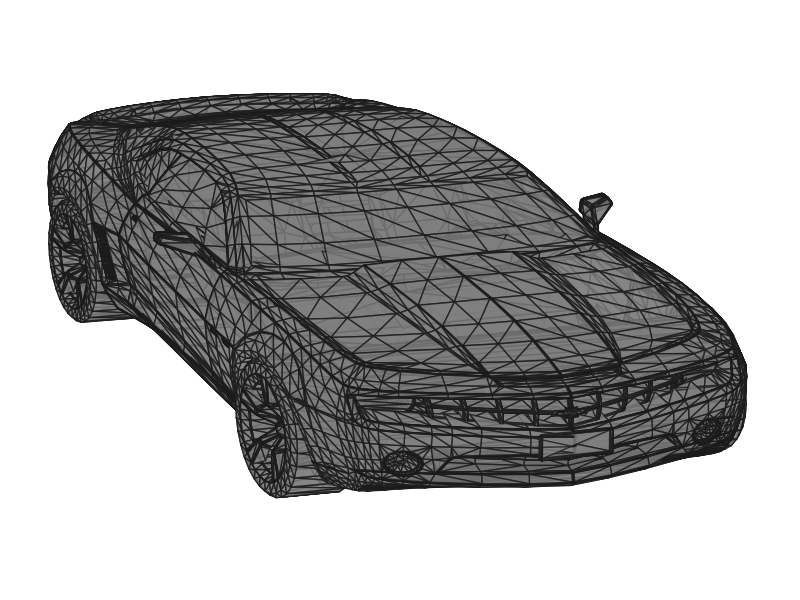
\includegraphics[width=3cm]{images/data/shapenet/simplification/1137cd58d6a45c6659a47b1880958de9}};
  %  \node at (3,-2.5) {\includegraphics[width=3cm]{images/data/shapenet/simplification/119033fe083145e22f31600ac759c763}};
    
  %  \node at (8,1.75) {Observations};
  %  \node[rectangle,draw=black] at (8,0.15) {\includegraphics[width=5.5cm]{images/data/kitti/snapshot_01_rect}};
    
  %  \node[rectangle,draw=black,minimum height=2.5cm,minimum width=5.75cm,draw=black] at (8, -2.75) {};
  %  \node at (6.625, -2.75) {
  %    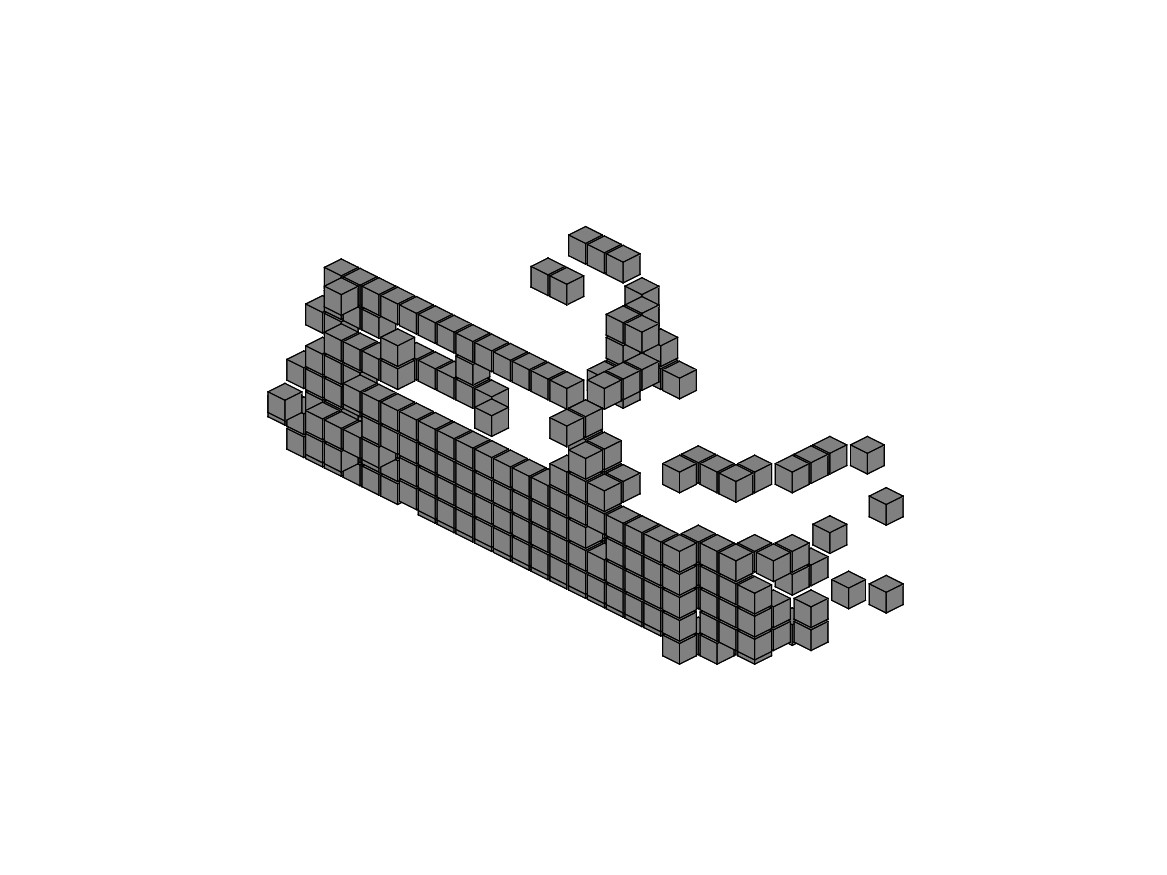
\includegraphics[width=2.75cm,trim={4.5cm 2.75cm 4.5cm 2.75cm},clip]{experiments/kitti/vae_occ_aml/15_long_statistics_combined/3_input_45}
  %  };    
  %  \node at (9.3725, -2.75) {
  %    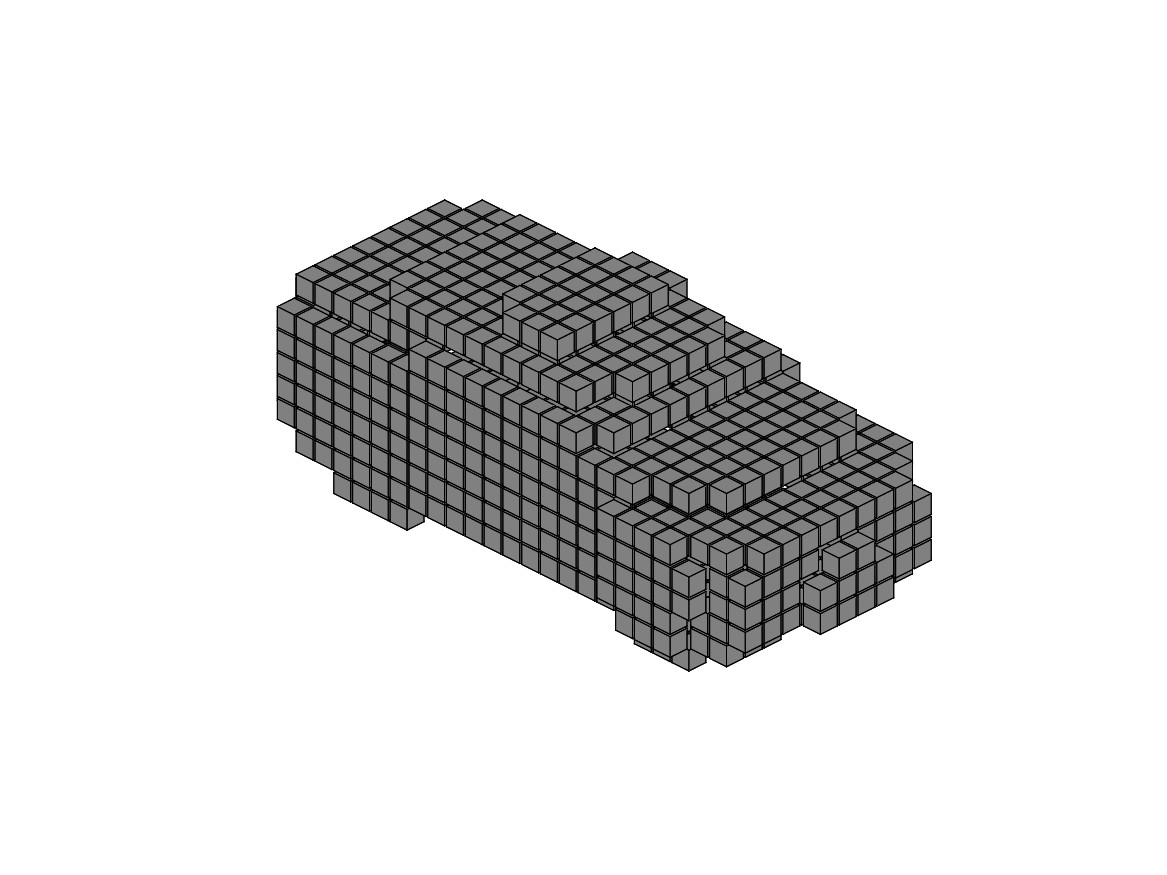
\includegraphics[width=2.75cm,trim={4.5cm 2.75cm 4.5cm 2.75cm},clip]{experiments/kitti/vae_occ_aml/15_long_statistics_combined/3_prediction_45}
  %  };
  %\end{tikzpicture}
  \vspace*{-1.25cm}
  \hspace*{-2cm}
  \begin{tikzpicture}
    \begin{scope}[on background layer]
      \node[rotate=45] at (-4,0.5) {
        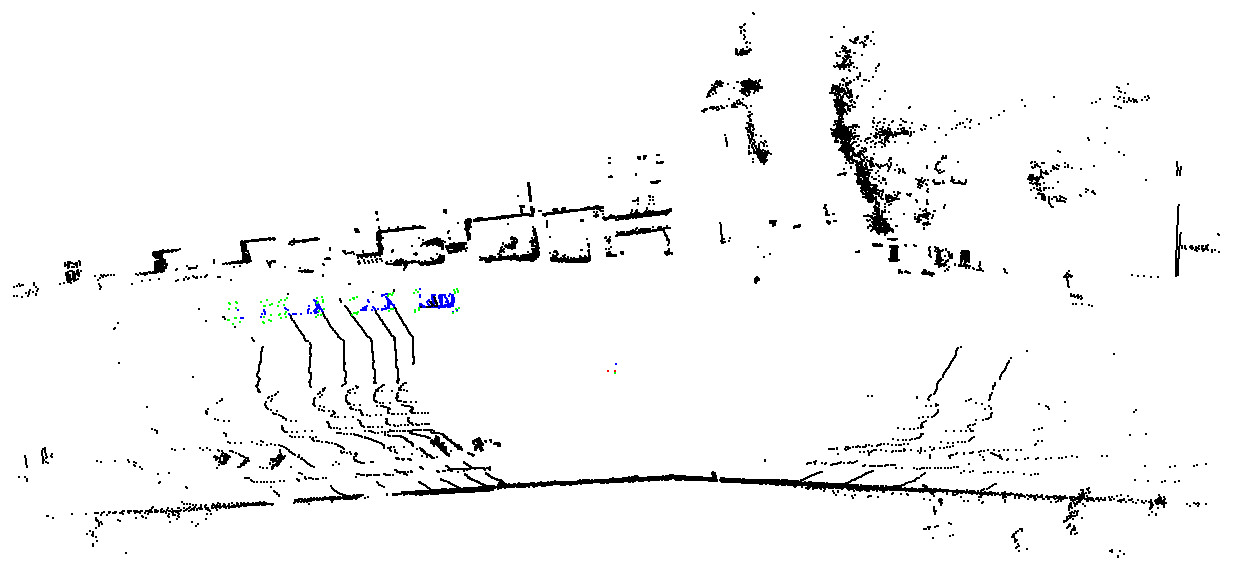
\includegraphics[width=8cm,trim={3cm 0 13cm 3cm},clip]{images/snapshot00_rect_fade}
      };
    \end{scope}
    
    \node[rectangle,draw=black,fill=white] at (3, 1.75) {
      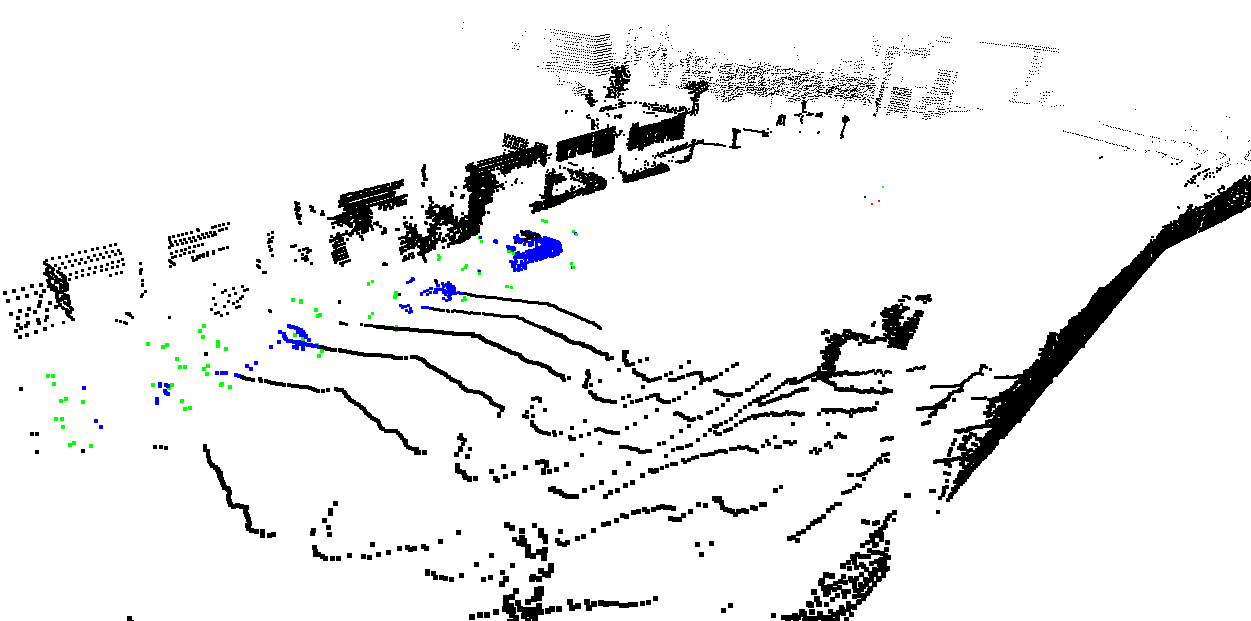
\includegraphics[width=8.85cm]{images/snapshot03_rect}
    };

    \node[rectangle,draw=black,fill=white] (input) at (0, -2) {
      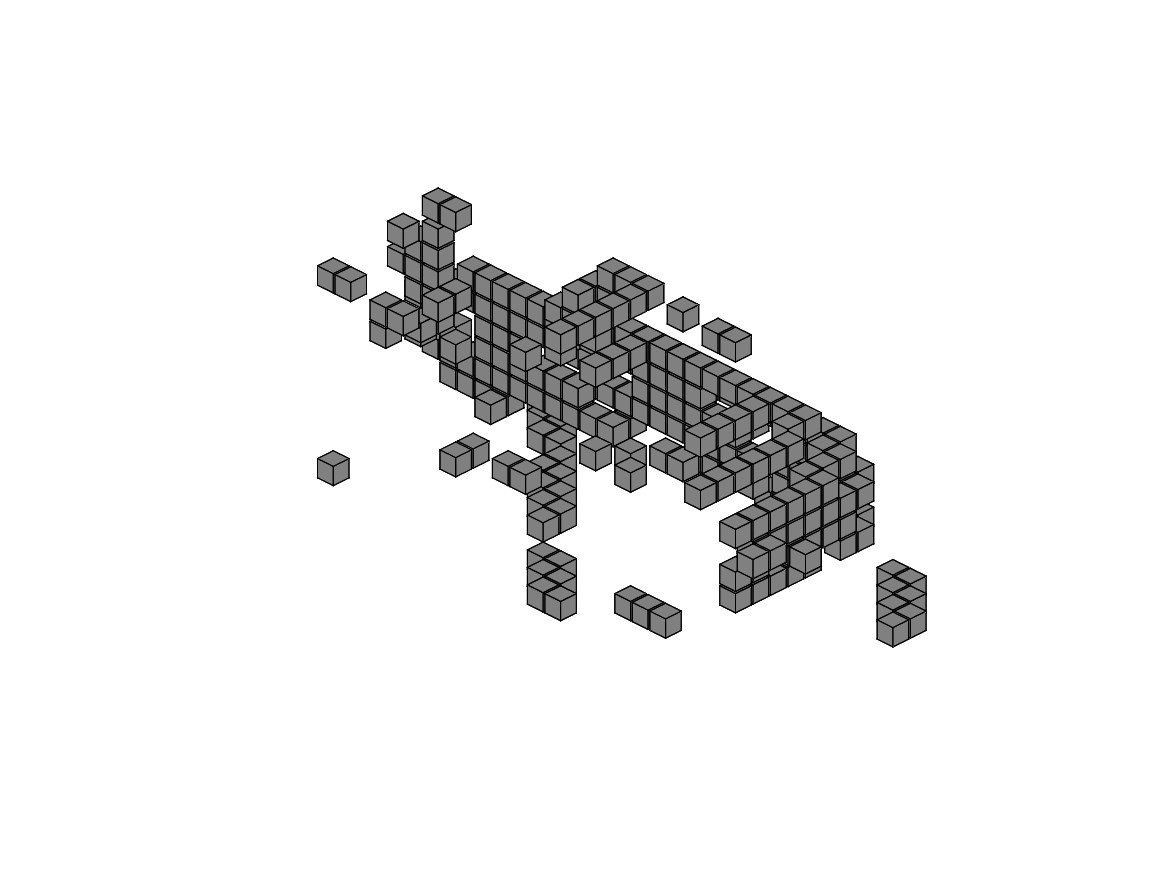
\includegraphics[height=2.25cm,trim={3cm 2cm 3cm 2cm},clip]{images/0_input_45}
    };
    \node at (0, -3.65) {\small Voxelized Observation};
    
    \node[rectangle,draw=black,fill=white] (output) at (6, -2) {
      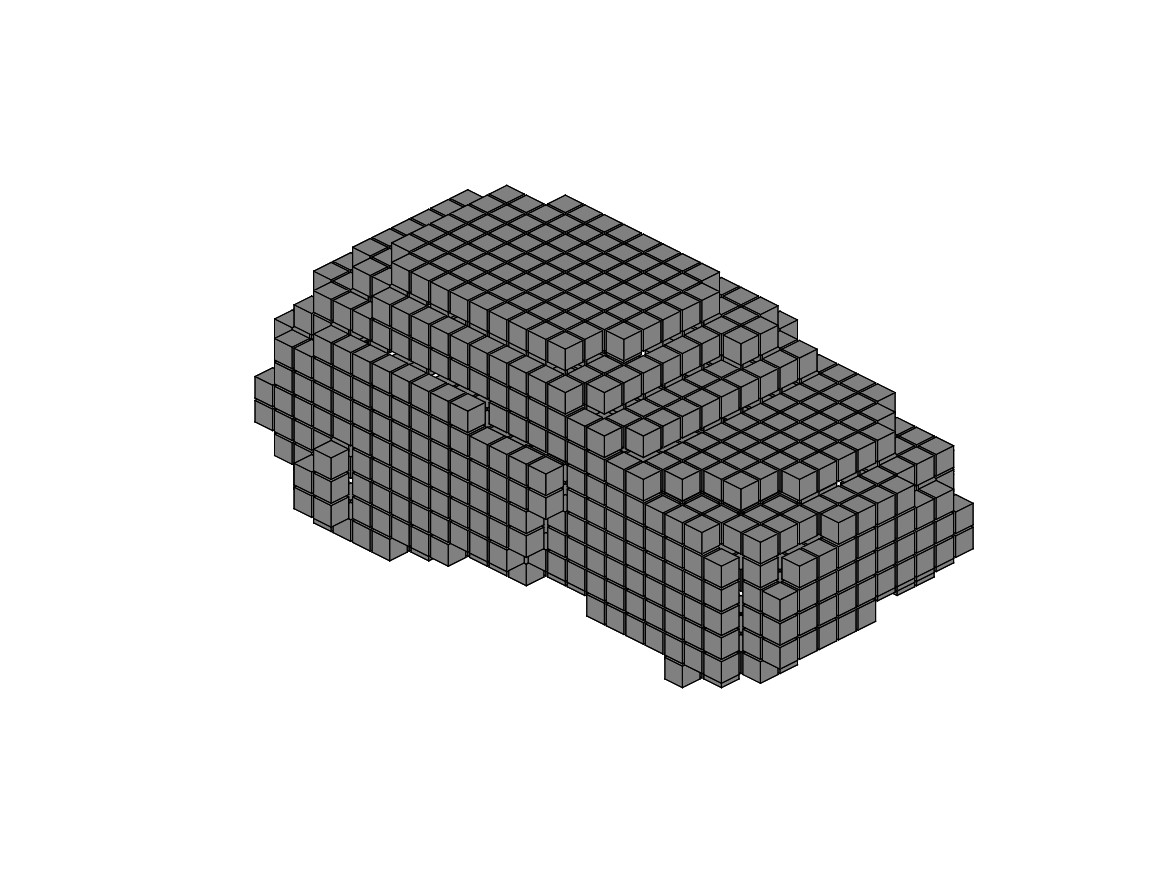
\includegraphics[height=2.25cm,trim={3cm 2cm 3cm 2cm},clip]{images/0_baseline_prediction_45}
    };
    \node at (6, -3.65) {\small Voxelized Shape};
    
    \draw[->] (input) -- (output);
    \node at (3, -1.4) {\small\begin{tabular}{c}Shape\\Completion\end{tabular}};
  \end{tikzpicture}
  \vspace{-0.5cm}
  
  % TODO short caption
  \caption{Illustration of the shape completion problem on
  KITTI \cite{GeigerLenzUrtasun:2012,GeigerLenzStillerUrtasun:2013} where we
  intend to learn shape completion of cars. We show a bird's eye view
  of a point cloud from KITTI in the background. On top, we show the same point cloud from
  a more natural viewpoint showing the points corresponding to cars
  in blue and the corresponding 3D bounding boxes, in particular their corners,
  highlighted in green. Below we show an illustration of the shape completion
  task. We extract point clouds of cars using the corresponding 3D bounding boxes
  and subsequently voxelize these points to obtain occupancy grids.
  Shape completion then describes the task of predicting a full shape which
  is also illustrated using occupancy grids, \ie in voxelized form.}
  \label{fig:introduction}
\end{figure}

In this thesis, we propose a probabilistic framework for shape completion
that tries to mitigate both problems: the need of annotated training data
%\cite{SmithMeger:2017,
%DaiNiessner:2016,SharmaFritz:2016,FanSuGuibas:2016,RezendeHeess:2016}
and the drawbacks of computationally involved optimization problems.
%\cite{EngelmannStuecklerLeibe:2016,BaoSavarese:2013,DameReid:2013}.
Following related work, \eg
\cite{SmithMeger:2017,GirdharGupta:2016,DaiNiessner:2016,
SharmaFritz:2016,BrockWeston:2016,WuSongXiao:2015} or \cite{WuTenenbaum:2016},
we utilize ShapeNet to learn
a strong shape prior using deep generative models, specifically variational
auto-encoders \cite{KingmaWelling:2013}. We hypothesize that using a strong
prior of possible shapes, we are able to learn how to complete shapes
under weak supervision, \ie only given knowledge about the object category
at hand. On real data, we additionally require knowledge about the object location
in the form of bounding boxes, \eg provided by an object detector.
By learning shape completion
using deep networks, we additionally reduce the problem to a forward pass
of the trained network.

\section{Contributions}

We propose two different probabilistic frameworks enabling us to learn
shape completion with weak supervision. In both cases, we first train
a shape prior, particularly a variational auto-encoder.
In the spirit of \cite{EngelmannStuecklerLeibe:2016}, we can then formulate
shape completion as maximum likelihood problem over the learned latent space.
Instead of maximizing the likelihood independently for distinct observations,
however, we follow the idea of amortized inference \cite{GershamGoodman:2014}
and learn to predict the maximum likelihood solution directly given the
corresponding observations. Specifically, we train an encoder,
which embeds the observations in the same latent space, using an unsupervised,
maximum likelihood loss between the observations and the corresponding shapes.
This variant of amortized maximum likelihood allows us to learn shape completion
under real conditions, \eg on KITTI,
and is able to compete with a fully-supervised baseline on a ShapeNet-based, synthetic dataset used for evaluation.

As alternative approach, we extend the general framework of latent space models,
as implemented by variational auto-encoders, to specifically account for the
observations. Applied to a pre-trained variational auto-encoder -- representing
the required shape prior -- we derive the evidence lower bound 
of this extended variational auto-encoder which we then
optimize in an unsupervised fashion, \ie only given the observations. We
also show that the underlying objective is closely related to
our amortized maximum likelihood approach. On our synthetic, ShapeNet-based dataset,
we experimentally demonstrate the applicability of the extended
variational auto-encoder regarding shape completion. Overall, we present two
approaches in favor of our claim that shape priors allow to learn shape completion
in an unsupervised fashion, thereby also introducing many interesting directions
for future research.

\section{Outline}

We formally introduce the problem of shape completion
under weak supervision in Chapter \ref{ch:problem}. Subsequently, Chapter
\ref{ch:related-work} reviews relevant related work. In Chapter \ref{ch:deep-learning},
we introduce the necessary background of training 3D convolutional neural networks.
We then discuss appropriate shape representations in Chapter 
\ref{ch:shape-representation}, before introducing the variational auto-encoder
which is used as shape prior. In Chapter \ref{ch:shape-inference},
we discuss how to use these models to learn shape completion with weak supervision.
The datasets used for our experiments are introduced in Chapter~\ref{ch:data}.
Finally, in Chapter \ref{ch:experiments},
we present experiments and conclude in Chapter \ref{ch:conclusion} including a
discussion of future work.

  \chapter{Problem}
\label{ch:problem}

We define shape completion as the surface reconstruction of a single object
from a known object category given a partial observation of its shape
-- usually from one view only.
As indicated in the introduction, we follow a learning-based approach.
In its simplest form, \ie the supervised case, the problem can be
stated as:

\begin{problem}%[Supervised Shape Completion]
  \label{problem:supervised}
  Given (partial) observations $\mathcal{X} = \{x_1,\ldots,x_N\} \subseteq \mathbb{R}^R$ and
  shapes $\mathcal{Y}^* = \{y^*_1, \ldots, y^*_N\} \subseteq \mathbb{R}^R$ of a specific
  object category such that
  $y^*_n$ represents the ground truth shape of $x_n$, the task is to learn a 
  mapping $x_n \mapsto y^*_n$ that is able to generalize to previously unseen
  observations.
\end{problem}

Here, we assume the observations $x_n$ and shapes $y^*_n$ to be vectors in
some high-dimensional space $\mathbb{R}^R$ for brevity of notation. In practice,
we will resort to occupancy grids or signed distance functions in three spatial
dimensions, \eg $x_n, y^*_n \in \mathbb{R}^{H \times W \times D} \simeq \mathbb{R}^R$.
The observations $x_n$ correspond to observed points -- either
occupied or non-occupied -- and unobserved points. In order to make explicit
that these are merely partial observations, we use $x_n \in \{0,1,\uk\}^R$
where $\uk$ corresponds to unobserved points.

Obtaining the ground truth shapes $\mathcal{Y}^*$ for real-world
observations $\mathcal{X}$ is labor-intensive
(\cf \cite{GuptaMalik:2015,MenzeGeiger:2015}).
Thus, the unsupervised version of Problem \ref{problem:supervised} can be formulated
as follows:

\begin{problem}%[Unsupervised Shape Completion]
  \label{problem:unsupervised}
  Given (partial) observations $\mathcal{X} = \{x_1,\ldots,x_N\} \subseteq \mathbb{R}^R$
  of a specific object category,
  the task is to learn a mapping $x_n \mapsto y(x_n) \in \mathbb{R}^R$ where
  $y(x_n)$ represents a shape that matches the unknown ground truth
  shape $y^*_n \in \mathbb{R}^R$ as close as possible.
\end{problem}

Problem \ref{problem:unsupervised} can also be interpreted as weakly-supervised
problem as we assume knowledge about the object category. However, this knowledge
is not used explicitly yet. Furthermore, both
Problem \ref{problem:supervised} and Problem \ref{problem:unsupervised} imply that
each observation $x_n$ corresponds to one individual object. This
means that we assume an object detector to be given in order to extract
the observations $x_n$ from full point clouds
as provided in real-world applications, \eg on KITTI
\cite{GeigerLenzUrtasun:2012,GeigerLenzStillerUrtasun:2013}.

\section{Proposed Approach}

Problem \ref{problem:unsupervised} is inherently ambiguous; in practice, infinitely
many shapes may match a given observation and even the ground truth
shape does not need to match the observation perfectly due to noise.
We propose a Bayesian approach in order to model this uncertainty appropriately.
As we assume knowledge of the object category, we collect a set
$\mathcal{Y} = \{y_1, \ldots,y_M\} \subseteq \mathbb{R}^R$ of representative shapes
corresponding to this object category.
In practice, this might correspond to a set of Computer-Aided Design (CAD) models,
\ie triangular meshes. Problem \ref{problem:unsupervised} is then re-stated below:

\begin{figure}
  \centering
  \begin{tikzpicture}
    \node[rectangle,draw=black,fill=white] at (-3, 0.7) {
      \includegraphics[height=1cm]{data/shapenet/simplification/119033fe083145e22f31600ac759c763}
    };
    \node[rectangle,draw=black,fill=white] at (-3, -0.7) {
      \includegraphics[height=1cm]{data/shapenet/simplification/119033fe083145e22f31600ac759c763}
    };
    \node[rectangle,draw=black,fill=white] at (-1.25, 0.7) {
      \includegraphics[height=1cm]{data/shapenet/simplification/119033fe083145e22f31600ac759c763}
    };
    \node[rectangle,draw=black,fill=white] at (-1.25, -0.7) {
      \includegraphics[height=1cm]{data/shapenet/simplification/119033fe083145e22f31600ac759c763}
    };
    \node at (-2.125, -1.75) {\small Shapes $y_m$};
    
    \node[rectangle,draw=black,fill=white] (input) at (1.4, 0) {
      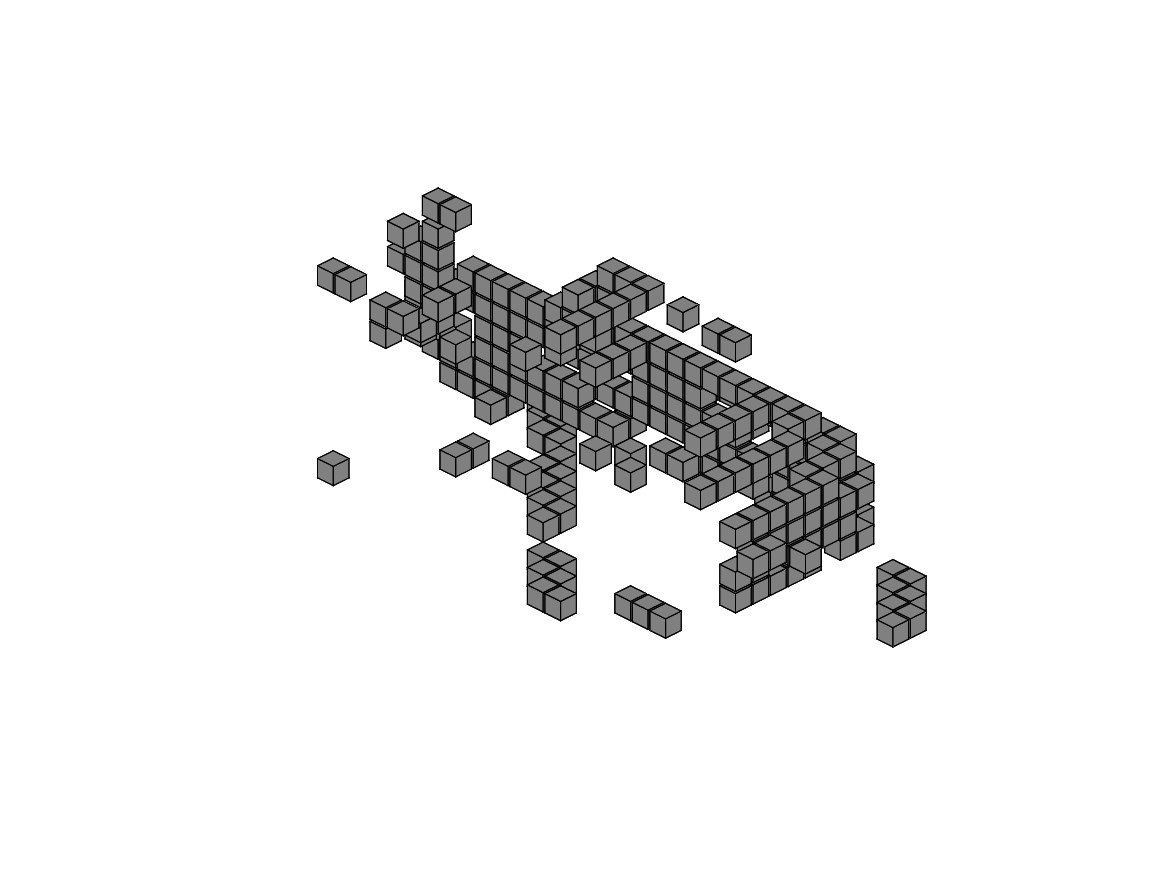
\includegraphics[height=2.4cm,trim={3cm 2cm 3cm 2cm},clip]{images/0_input_45}
    };
    \node at (1.4, -1.75) {\small Observation $x_n$};
    
    \node[rectangle,draw=black,fill=white] (output) at (8, 0) {
      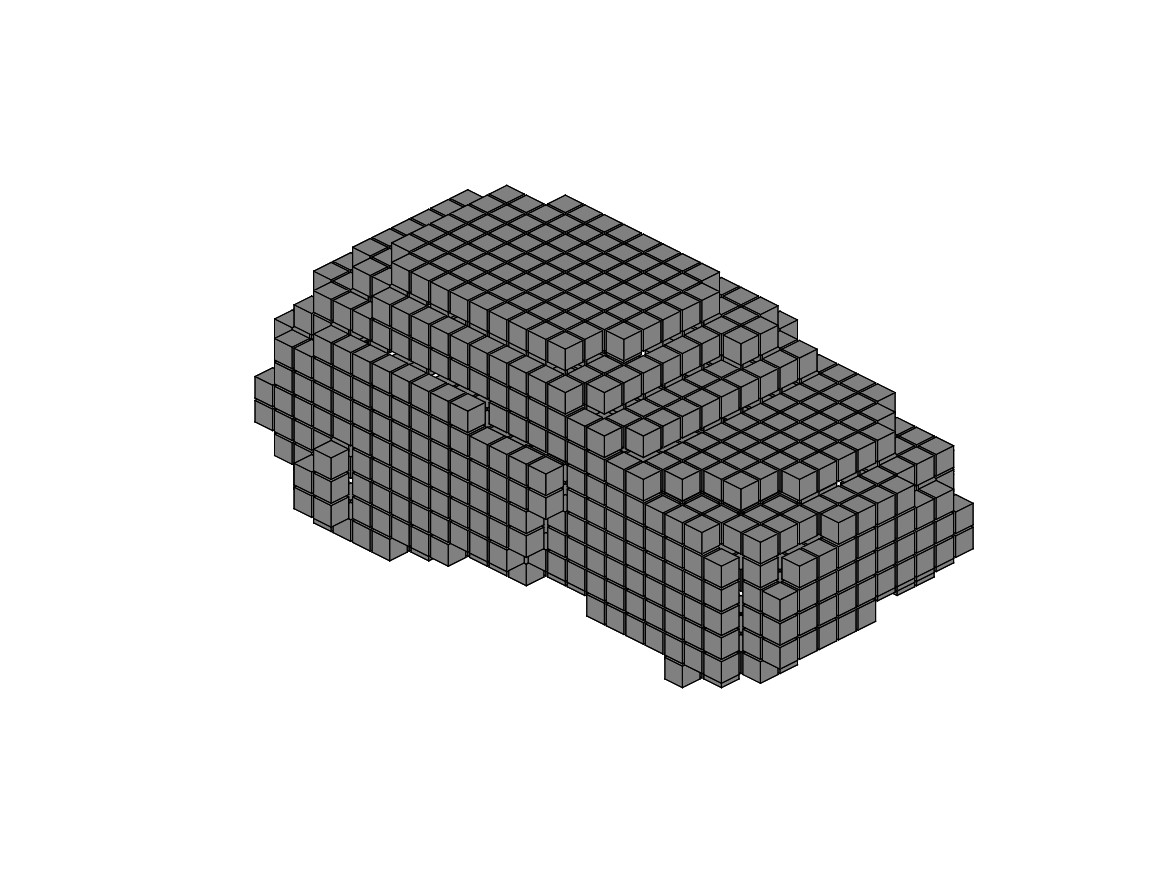
\includegraphics[height=2.4cm,trim={3cm 2cm 3cm 2cm},clip]{images/0_baseline_prediction_45}
    };
    \node at (8, -1.75) {\small Shape $y_n^*$};
    
    \node at (4.6, 0.65) {\small \begin{tabular}{c}Shape\\Completion\end{tabular}};
    \draw[->] (input) -- (output);
  \end{tikzpicture}
  \caption{An illustration of Problem \ref{problem}; the set of reference shapes
  $\mathcal{Y}$ is usually provided in the form of triangular meshes, \eg from
  ShapeNet \cite{ChangFunkhouserGuibasSavarese:2015}. After voxelization, these
  are used to learn a shape prior. The problem of shape completion is then
  illustrated by showing a voxelized observation $x_n$ and the
  corresponding ground truth, \ie completed, shape $y_n^*$.}
  \label{fig:problem}
\end{figure}

\begin{problem}%[Weakly-Supervised Shape Completion]
  \label{problem}
  Given (partial) observations
  $\mathcal{X} = \{x_1,\ldots,x_N\} \subseteq \mathbb{R}^R$
  and shapes $\mathcal{Y} = \{y_1, \ldots,y_M\} \subseteq \mathbb{R}^R$ of a specific object
  category, the task is to learn a mapping $x_n \mapsto y(x_n) \in \mathbb{R}^R$
  such that $y(x_n)$ matches the unknown ground truth
  shape $y^*_n \in \mathbb{R}^R$ as close as possible.
\end{problem}

We propose to use the set $\mathcal{Y}$ to learn a prior of possible shapes, \eg
using a variational auto-encoder. Shape completion can then be formulated as maximum
likelihood problem over a lower-dimensional latent space $\mathcal{Z} = \mathbb{R}^Q$,
$Q \ll R$. To this end, we interpret the individual voxels $y_i$, for $y \in \mathbb{R}^R$,
as random variables and $x_i$, for $x \in \mathbb{R}^R$, as the corresponding observations.
Then, $\mathcal{Y}$ is used to learn a prior model $p(y, z)$ which
decomposes into a generative model and a prior: $p(y, z) = p(y | z) p(z)$.
Using the set of observations $\mathcal{X}$, we then train an inference model
that directly learns the mapping
\begin{align}
  x \mapsto \tilde{z} = \argmax_{z} p(y = x | z) p(z).\label{eq:problem}
\end{align}
thereby implicitly solving Problem \ref{problem}. We interpret this approach
as amortized maximum likelihood following the idea of \cite{GershamGoodman:2014}.
In particular, we do not consider the maximum likelihood problem for each
observation $x$ independently. Instead, we understand the maximum likelihood
problem as loss between observations and shapes allowing to learn the
embedding $x \mapsto \tilde{z}$ in an unsupervised fashion. In the context
of variational auto-encoders, this boils down to training a new encoder to
represent the embedding of observations within the latent space.

Alternatively, we can consider the observations $x_i$ to be random variables, as well.
For the joint probability of the model, \ie $p(x, y, z)$, we can subsequently
derive the evidence lower bound. Using the simplifying assumption that $y$ and
$z$ are statistically independent given $x$, % \ie $q(y, z | x) = q(y | x) q(z | x)$,
we can use an extended variational auto-encoder to implicitly learn an approximate
model $q(z | x)$ which, again,
implicitly solves Problem \ref{problem}. Here, instead of directly
optimizing the maximum likelihood in Equation \eqref{eq:problem} (involving
$p(y = x | z)$), the observations are tied to the corresponding shapes through
a Kullback-Leibler divergence.
%In particular, the Kullback-Leibler
%divergence $\KL(q(y | x) | p(y | z))$ is minimized in order to learn
The learned model $q(z | x)$ can then be interpreted as a probabilistic embedding
of the observations in the latent shape space, in analogy to the
mapping $x \mapsto \tilde{z}$ learned when amortizing maximum likelihood.
Overall, both approaches require a shape prior defining a latent space
of shapes and subsequently learn to embed the partial observations within
this space.

  \chapter{Related Work}
\label{ch:related-work}

In this chapter, we intend to provide a concise but structured discussion
of related work. We first consider the shape completion task itself, focusing
on data-driven and learning-based approaches that are most related to our approach.
We also discuss the use of shape priors in general, \eg for tasks including
3D reconstruction, 3D pose estimation or tracking. Finally, we give a brief
overview of 3D deep learning, specifically regarding generative shape models,
as well as the idea of amortized inference. We note, however, that we do not intend
to provide a comprehensive discussion of these areas due to time and space constraints.

\section{Shape Completion}

% PhDs:
% - Martin Oswald (http://people.inf.ethz.ch/moswald/publications/resources/Oswald-MR-PhD-Thesis.pdf)
% - Kalin Kolev
% - Christian Häne
% - Marc Pollefeys (https://www.inf.ethz.ch/personal/pomarc/pubs/PollefeysPhD.pdf)
Shape completion is closely related to 3D reconstruction as well as
surface reconstruction; however, the addressed problems
do usually not exactly match the problem of shape completion.
Therefore, we refer to recent textbooks
\cite{ForsythPonce:2012, Szeliski:2011} and surveys
\cite{MoonsVanGoolVergauwen:2010,FurukawaHernandez:2015,
BergerSilva:2014,BrecksonFisher:2005}
for a general overview of these fields.

In contrast to surface reconstruction and 3D reconstruction, shape completion
is usually performed on partial scans of individual objects.
Following \cite{SungAngstGuibas:2015}, shape completion approaches
can roughly be categorized into data-driven methods and symmetry-based
methods.
The latter detect symmetry in non-occluded parts in order to complete shapes
by completing the corresponding symmetry in occluded parts; representative works
are \cite{ThrunWegbreit:2005,PaulyGuibas:2008,ZhengChen:2010,KroemerPeters:2012}
or \cite{LawAliaga:2011}. These approaches also found application in robotics,
\eg for robot grasping \cite{KroemerPeters:2012,MartonRusuBeetz:2009}.
The data-driven case is more interesting
in relation to the proposed approaches; in early work, Pauly \etal
\cite{PaulyGuibas:2005} pose shape completion as retrieval and
alignment problem. Further work in this direction includes \eg
\cite{LiDaiGuibasNiessner:2015,NanSharf:2012,GuptaMalik:2015,DameReid:2013,
EngelmannStuecklerLeibe:2016,EngelmannLeibe:2017} where 
local shape features \cite{LiDaiGuibasNiessner:2015,NanSharf:2012},
object knowledge \cite{GuptaMalik:2015,DameReid:2013} or shape priors
\cite{EngelmannStuecklerLeibe:2016,EngelmannLeibe:2017,DameReid:2013} have found application.
Model fitting often follows a scheme similar to the
iterative closest point (ICP) algorithm \cite{BeslMcKay:1992} or is posed
as energy minimization. We also refer to \cite[Table~1]{BergerSilva:2014}.

Recently, several learning-based approaches have been proposed
\cite{RieglerGeiger:2017,FirmanBrostow:2016,SmithMeger:2017,DaiNiessner:2016,SharmaFritz:2016,
RezendeHeess:2016,FanSuGuibas:2016}, most of them using deep learning.
Shape completion is posed as supervised learning problem, \eg from single RGB(-D)
images \cite{FanSuGuibas:2016,GirdharGupta:2016}, partial observations
\cite{RieglerGeiger:2017,DaiNiessner:2016,RezendeHeess:2016,SmithMeger:2017},
or noisy shapes \cite{SharmaFritz:2016}. In comparison with data-driven approaches,
shape completion usually involves a single forward pass of the trained network.
However, these approaches can only be applied on synthetic datasets such as
ModelNet \cite{WuSongXiao:2015} or ShapeNet \cite{ChangFunkhouserGuibasSavarese:2015}
as explicit supervision is required. We also intend to leverage deep neural networks,
however, we want to learn shape completion in a weakly supervised setting
only using the given observations and knowledge about the object category.
This allows us to learn shape completion on real data, \eg on KITTI
\cite{GeigerLenzUrtasun:2012,GeigerLenzStillerUrtasun:2013}, while still
providing efficient inference through the trained network.

\subsection{Shape Priors}

As indicated above, shape priors play an important role in shape completion.
For example, learning-based approaches can be
understood as implicitly learning a shape prior from supervised training data
\cite{RieglerGeiger:2017,SmithMeger:2017,DaiNiessner:2016,SharmaFritz:2016,
RezendeHeess:2016,FanSuGuibas:2016}. Only \cite{GirdharGupta:2016} uses
the learned shape model explicitly to constrain the space of
predicted shapes. Data-driven methods may also make use of learned shape priors, \eg
using principal component analysis (PCA) \cite{EngelmannStuecklerLeibe:2016,EngelmannLeibe:2017}
or Gaussian process latent variable models (GP-LVM) \cite{DameReid:2013}.
However, shape priors have also been applied in different domains,
\eg in 3D pose estimation -- often tackled in conjunction with
tasks such as image segmentation \cite{AdrianReid:2012,DambrevilleTannenbaum:2008,
SandhuTannenbaum:2009} or scene flow \cite{MenzeHeipkeGeiger:2015}.
Shape priors have also become a standard tool in tracking, see \cite{MaSibley:2014}
or \cite{LeottaMundy:2009} for related work in this domain.
In classical 3D reconstruction, shape priors are also commonly used to resolve \eg ambiguities
\cite{GueneyGeiger:2015}, specularities \cite{DameReid:2013} or the lack of
texture \cite{BaoSavarese:2013}.
In most cases, shape priors are ``learned'' from full shapes; this is in contrast
to non-data-driven priors such as local or global smoothness priors,
planarity assumptions \etc, see \cite{BergerSilva:2014}.
We mostly follow the idea of \cite{EngelmannStuecklerLeibe:2016,EngelmannLeibe:2017,
DameReid:2013} or \cite{GirdharGupta:2016} and use a shape prior explicitly to
define and constraint the space of possible shapes.

\section{3D Deep Learning and Amortized Inference}

In computer vision, deep learning often refers to the practice of using
deep convolutional neural networks \cite{LeCunBoserDenkerHenderson:1989}
to train discriminative and more recently also generative models. 
While neural networks have been used and researched for several decades now (\eg see
\cite{Bishop:1995,Haykin:2005,Rosenblatt:1958,RumelhartHintonWilliams:1986,
HornikStinchcombeWhite:1989}), they only recently received considerable attention.
Among several milestones is the substantial performance increase on the ImageNet
classification challenge \cite{DengFeiFei:2009} in 2012 \cite{KrizhevskySutskeverHinton:2012}.
Afterwards, deep convolutional neural networks have been successfully applied
to a wide range of computer vision tasks -- more complete overviews can be found in
\cite{Schmidhuber:2014,WangRajXing:2017,Li:2017,
BengioCourvilleVincent:2012,LeCunBengioGeoffrey:2015,
GoodfellowBengioCourville:2016}.

Recently, deep generative models, \eg
\cite{VanDenOordKavukcuoglu:2016,VanDenOordGraves:2016,GoodfellowBengio:2014,
MakhzaniGoodfellow:2015,KingmaWelling:2013,LarsenWinther:2016}
and related work, have received considerable attention. Such models offer
to generate realistic images or shapes and to learn strong prior models
which are interesting for semi-, weakly- or unsupervised tasks, \eg in
\cite{KingmaMohamedRezendeWelling:2014}. In this thesis, we will use variational
auto-encoders and subsequent work \cite{ImAhnMemisevicBengio:2017,JangGuPoole:2016,MaddisonMnihTeh:2016} as they
include both an inference and a generative model. This is also motivated by
the fact that generative adversarial networks \cite{GoodfellowBengio:2014}
are known to be hard to train
\cite{MeschederGeiger:2017,NowozinTomioka:2016,SalimansGoodfellowChen:2016,
GulrajaniCourville:2017,ArjovskyBottou:2017},
%\footnote{
%  \url{https://github.com/soumith/ganhacks}
%}
a problem that we anticipated to be amplified on 3D data. Generative models
have also been applied to shape modeling, \eg
\cite{SmithMeger:2017,GirdharGupta:2016,%DaiNiessner:2016,SharmaFritz:2016,
BrockWeston:2016,WuSongXiao:2015,WuTenenbaum:2016}, allowing
shape interpolation, manipulation and generation.

\subsection{3D Deep Learning}

Most works, including \cite{WuTenenbaum:2016,SmithMeger:2017,WuSongXiao:2015,
BrockWeston:2016,SharmaFritz:2016,DaiNiessner:2016,GirdharGupta:2016,
GarciaGarciaLopez:2016,MaturanaScherer:2015}, naively
generalize convolutional neural networks to 3D data, \eg in the form of voxelized shapes.
Unfortunately, this significantly limits the used resolution; usually resolutions between
$32^3$ and $64^3$ are used. Some approaches, however, exploit the sparsity of
3D data through octrees, \eg
\cite{WangTong:2017,RieglerGeiger:2016,RieglerGeiger:2017,TatarchenkoBrox:2017},
to reduce memory and time consumption and allow higher resolutions, \eg up to
$256^3$ \cite{RieglerGeiger:2016}. Alternatively, sparse convolution schemes have
been defined to speed up training \cite{LiGuibas:2016,EngelckePosner:2017,Graham:2015}.
There is also a line of work applying convolutional neural networks directly to meshes
\cite{GuoChen:2015,BoscainiVandergheynst:2015,BrunaLeCun:2013}
or point clouds \cite{QiSuGuibas:2016a,FanSuGuibas:2016,QiYiSuGuibas:2017}. While we also
use simple 3D convolutional neural networks for the presented experiments,
which we also conduct on a resolution of $32^3$, the above references provide
interesting possibilities for future work.

\subsection{Amortized Inference}

% https://arxiv.org/pdf/1611.01722.pdf
% http://gershmanlab.webfactional.com/pubs/GershmanGoodman14.pdf
% https://arxiv.org/pdf/1505.05770.pdf
To the best of our knowledge, the notion of amortized inference
was first introduced in \cite{GershamGoodman:2014}, however, has been used repeatedly
in recent work
\cite{KingmaWelling:2013,RezendeMohamed:2015,WangLiu:2016,
RezendeMohamedWierstra:2014,RitchieGoodman:2016}. While a clear, coherent definition
is still missing, amortized inference generally describes the idea of learning
inference, \eg in the form of ``learning to sample'' \cite{WangLiu:2016}
or amortized, \ie learned, variational inference \cite{KingmaWelling:2013,
RezendeMohamed:2015}. The idea includes that drawn samples -- or past inferences -- 
are not considered independently; instead, inference can profit from insights
obtained from past inferences. In our case, we learn, \ie amortize, the 
maximum likelihood problem for shape completion.

  \chapter{Deep Learning}
\label{ch:deep-learning}

Deep learning generally describes the use of deep neural networks
\cite{GoodfellowBengioCourville:2016} -- where depth may refer to both the number of model
parameters as well as the number of used layers, \ie processing steps.
In the context of this thesis, neural networks are used in the framework
of variational auto-encoders to learn the shape prior, \ie the embedding
of shapes $\mathcal{Y}$ within a latent space $\mathcal{Z}$. Specifically,
both the generative model $p(y | z)$ and the approximate recognition model
$q(z | y)$ are implemented using neural networks.
This is accomplished by choosing appropriate parameterizations and predicting
the corresponding parameters -- \eg mean and variance for Gaussian distributions.
In the proposed approaches, neural networks will also be used to learn the embedding
of observations $x$ in the latent shape space. For amortized maximum likelihood,
this will be a deterministic embedding $x \mapsto z(x;w)$ -- here, we
made the parameters $w$ of the neural network explicit. For the proposed
extended variational auto-encoder, the embedding is represented by the
approximate recognition model $q(z | x)$.

In general, neural networks can be introduced from different viewpoints (\cf
\cite{Bishop:2006,DudaHartStork:2001,Bishop:1995,Haykin:2005,GoodfellowBengioCourville:2016}).
In this chapter, we follow \cite{GoodfellowBengioCourville:2016} 
and introduce neural networks as series (or acyclic graph, in general) of
tensor operations which use a set of parameters $w$ in order to -- given input $x$ --
compute a function $y(x;w)$ that may approximate some target function.
We will first introduce the used concept of tensors -- the data structure
underlying all modern deep learning frameworks -- before gradually
defining more complex networks and finally discussing network training.

\section{Tensors}

In our context, real tensors are generally understood as multi-dimensional arrays
\cite[Section~2.1]{GoodfellowBengioCourville:2016} of real numbers:
%We note that the presented concept of tensors does not
%necessarily match the concept of tensors in mathematics or physics\footnote{
%  We refer the reader to this lively discussion with many good examples:
%  \url{http://stats.stackexchange.com/questions/198061/why-the-sudden-fascination-with-tensors}.
%}.

\begin{definition}%[Tensor]
  A (real) tensor is an element $t \in \mathbb{R}^{n_1 \times \ldots \times n_r}$
  where $(n_1,\ldots,n_r) \in \mathbb{N}^r$ and $r$ is called the rank of the tensor.
  We write $r_i := r_{(i_1,\ldots,i_r)}$ to index a tensor; in this case,
  $i = (i_1, \ldots, i_r)$ is called multi-index.
\end{definition}

In practice, the rank is often referred to as dimension. While this is mathematically
imprecise, we will use both interchangeably. Thus, a tensor
$t \in \mathbb{R}^{n_1 \times \ldots \times n_r}$ has dimension (=rank) $r$ and
$n_i$ is called the size of dimension $i$. We also allow so-called singleton dimensions,
\ie dimensions of size $1$. Then, the terminology can be applied one-to-one
to many popular deep learning frameworks such as Torch, PyTorch, Theano,
Tensorflow, Caffe and more\footnote{
  \url{http://torch.ch/}, \url{http://pytorch.org/}, \url{https://github.com/Theano/Theano}, \url{https://www.tensorflow.org/} and \url{http://caffe.berkeleyvision.org/}.
}.

\begin{example}
  Examples include trivial cases such as scalars, \ie rank-$0$ tensors, vectors,
  \ie rank-$1$ tensors, and matrices, \ie rank-$2$ tensors. Examples specific to
  our problem include:
  \begin{description}
    %\item[Scalar] A scalar is a tensor of rank $0$.
    %\item[Vector] A vector $t \in \mathbb{R}^C$ is a rank $1$ tensor.
    %\item[Matrix] A matrix $t \in \mathbb{R}^{H \times W}$ is a rank $2$ tensor
    %where $H$ is the number of rows and $W$ the number of columns.
    %\item[Image] A rank-$2$ tensor $t \in \mathbb{R}^{H \times W}$
    %can be interpreted as grayscale (or single-channel) image of height
    %$H$ and width $W$.
    %In practice, the intensity of each pixel is usually encoded as 
    %8-bit number in $[0,255]$.
    \item[Multi-Channel Image] An image is a tensor of rank $3$:
    $t \in \mathbb{R}^{C \times H \times W}$ where $C$ is the number of channels,
    $H$ the height of the image and $W$ the width of the image.
    For grayscale (\ie single-channel) images, $C = 1$, while color images use
    $C = 3$ channels usually corresponding to red, green and blue. Grayscale as
    well as color is usually encoded using 8-bit each.
    %In deep learning, the different channels may also be
    %the result of intermediate feature computations on the image.
    \item[Multi-Channel Volumes] A tensor $t \in \mathbb{R}^{C \times H \times W \times D}$
    of rank $4$ can be interpreted as $C$-channel volume where $H$, $W$ and $D$ represent
    height, width and depth, respectively.
    Volumes are commonly used in medical imaging (\ie MRI or CT volumes). In our case,
    we use volumes to represent shapes using occupancy grids or (signed)
    distance functions, see Chapter \ref{ch:shape-representation}.
    %\item[Multi-Channel Volumes] Multi-channel volumes are represented by
    %rank $4$ tensors $t \in \mathbb{R}^{C \times H \times W \times D}$. In addition
    %to the spatial dimensions, $C$ channels are included.
    \item[Batch of Multi-Channel Volumes] A batch, \ie a set, of multi-channel volumes
    can be interpreted as tensor of rank $5$:
    $t \in \mathbb{R}^{B \times C \times H \times W \times D}$ where $B$ is
    the size of a set of multi-channel volumes. When training neural networks,
    $B$ will be the batch-size.
  \end{description}
\end{example}

In this thesis, we will mostly work with volumes and multi-channel volumes
and -- during training -- with batches of these. Therefore, 
we always consider the rank-$5$ case and usually refer to the
dimensions as $B \times C \times H \times W \times D$.
%All of the introduced concepts easily generalize to the case of tensors with
%different rank.

\subsection{Basic Tensor Operations}

% TODO cite tensor contraction
For tensors of rank $1$ or $2$ we can apply all the operations known from
linear algebra (\eg matrix-vector or matrix-matrix multiplications). 
Additionally, we define element-wise operations which are commonly
used in deep learning:

\begin{definition}
  Let $t, s$ be two tensors; let $i \in \mathbb{N}^5$ be a multi-index. Further,
  let $\times$ be any binary arithmetic operation on $\mathbb{R}$. Then the corresponding
  element-wise operation is defined by $(t \times s)_{i} = t_{i} \times s_{i}$.
\end{definition}

\begin{definition}
  Let $t$ be a tensor and $i \in \mathbb{N}^5$ be a multi-index; further, let
  $h : \mathbb{R} \mapsto \mathbb{R}$ be a real-valued function.
  Then, $h$ may operate element-wise on $t$, \ie $h(t)_i = h(t_i)$.
\end{definition}

\section{Layered Neural Networks}

In the following, we introduce layered neural networks -- models consisting
of several layers, \ie a sequence, of tensor operations. We follow the 
introduction of \cite[Chapter~6]{GoodfellowBengioCourville:2016}:

\begin{definition}
  \label{def:deep-learning-graph}
  A (feed-forward, layered) neural network is a directed, acyclic graph
  $G = (V, E)$ where each node $v \in V$ corresponds to an operation
  mapping one or more input tensors to one or more output tensors.
  The edges $(v_i, v_j) \in E$ characterize the information flow, \ie one
  or more of the output tensors of operation $v_i$ are fed as input into
  operation $v_j$. The operations
  $v_i$ are also called layers and may have a finite number of adjustable
  weights.
\end{definition}

% TODO wording, details ...
Given a topological ordering -- see \cite[Chapter~22]{Cormen:2009} -- of the
vertices $V = (v_{i_1}, \ldots, v_{i_{|V|}})$, the network computes its output
by sequentially computing the layers' outputs given an input $x$, \ie
$v_{i_1}(x)$, $v_{i_2}(v_{i_1}(x), x), v_{i_3}(v_{i_2}(v_{i_1}(x)), v_{i_1}(x), x)$, ...
An early example of a one-layer neural network is the perceptron \cite{Rosenblatt:1958}:

\begin{example}
  The perceptron is a linear classifier (\cf \cite[Chapter~4]{Bishop:2006}):
  $y(x;w) = x w^T$ where $x \in \mathbb{R}^{1 \times C}$ is an input tensor and
  $w \in \mathbb{R}^{1 \times C}$
  is a weight vector. Classification is done by considering $\sign y(x;w)$
  with class labels in $\{-1,1\}$. While the
  inner product $x w^T$ might be unintuitive,
  it allows to easily apply the decision function
  to a batch of samples $x_1,\ldots,x_B$ stacked into $x \in \mathbb{R}^{B \times X}$.
  %As we will see later, this formulation is also beneficial for training the weights
  %$w$.
\end{example}

Today the perceptron is more important than ever because it describes the
basic building blocks of neural networks, the fully connected layer:

\begin{definition}
  A fully connected layer, denoted $\text{fc}_{\Cin, \Cout}$
  takes as input a tensor $x \in \mathbb{R}^{B \times \Cin}$ and computes:
  \begin{align}
    \text{fc}_{\Cin,\Cout}(x) = x w^T \in \mathbb{R}^{B \times \Cout}
  \end{align}
  where $w \in \mathbb{R}^{\Cout \times \Cin}$ is the corresponding weight matrix.
\end{definition}

Usually, the fully connected layer is combined with an additive bias term:
\begin{align}
  y(x;w) = x w^T + \left[\begin{matrix}b\\\vdots\end{matrix}\right]
\end{align}
with $x \in \mathbb{R}^{B \times \Cin}$, $b \in \mathbb{R}^{1 \times \Cout}$
(which is repeated $B$ times to allow operations on batches) and,
as before, $w \in \mathbb{R}^{\Cout \times \Cin}$. 
To make this additive term explicit, we use a separate layer.
The bias layer can easily be generalized to tensors of higher rank and
is usually followed by non-linearity:

%\begin{definition}
%  A bias layer, denoted $\text{bias}$ takes as input an arbitrary tensor
%  $x \in \mathbb{R}^{B \times C}$ and adds a bias weight $w \in \mathbb{R}^{1 \times C}$
%  to each element in the batch:
%  \begin{align}
%    \text{bias}(x) = x + \left[\begin{matrix}w\\\vdots\end{matrix}\right].
%  \end{align}
%\end{definition}

%The fully connected layer (and bias layer if applicable) is usually followed by
%a non-linearity, this can also be motivated using the perceptron:

%\begin{example}
%  \label{ex:deep-learning-sigmoid}
%  For multi-class problems the decision function $\sign y(x;w)$ is usually problematic
%  as it allows regions in the input space where inputs $x$ are not assigned to 
%  any class -- this occurs both for one-vs-all and one-vs-one classifiers \cite{Bishop:2006}.
%  Therefore, the posteriors
%  \begin{align}
%    y_k(x;w) \approx p(y^*_k = 1 | x)
%  \end{align}
%  are modeled instead. This can be achieved by using
%  \begin{align}
%    y(x;w) = \sigma(x w^T)
%  \end{align}
%  with $x \in \mathbb{R}^{1 \times C}$, $w \in \mathbb{R}^{K \times C}$
%  with $K$ being the number
%  of classes and
%  \begin{align}
%    \sigma(x) = \frac{1}{1 + \exp(-x)}\label{eq:deep-learning-sigmoid}
%  \end{align}
%  being the logistic sigmoid.
%\end{example}

%Furthermore, non-linearity layers are motivated by the wish to
%approximate complex non-linear functions. Work from the late 80s
%\cite{HornikStinchcombeWhite:1989} shows that stacking perceptrons with non-linearities
%allows to approximate any continuous function.

%The element-wise application of non-linear functions can be formalized
%as layer as follows:

\begin{definition}
  Let $h : \mathbb{R} \mapsto \mathbb{R}$ be a real-valued function.
  Then, $h$ also denotes a layer taking as input an arbitrary tensor $x$
  and computing $h(x)$ element-wise.
\end{definition}

These non-linearities are also called activation or transfer functions
(\cf \cite{Bishop:1995,Haykin:2005,GoodfellowBengioCourville:2016})
and are motivated by the wish to approximate complex non-linear functions
\cite{HornikStinchcombeWhite:1989} using a combination of simpler,
non-linear functions.

\begin{example}
  Common non-linearities for neural networks include the logistic sigmoid
  \begin{align}
    \sigma(x) = \frac{1}{1 + \exp(-x)}
  \end{align}
  and the rectified linear unit $\ReLU(x) = \max(x, 0) = [x]_+$.
  %Other common activation functions include the hyperbolic tangent,
  %and variants of $\ReLU$ \cite{HeZhangRenSun:2015}.
  The logistic sigmoid allows to model probabilities and
  $\ReLU$ non-linearities have been shown
  to reduce training time and improve performance
  \cite{KrizhevskySutskeverHinton:2012,SzegedyRabinovich:2015} while being
  a good model of biological neurons \cite{GlorotBengio:2011}.
\end{example}

Finally we discuss our first layered neural network whose network graph
is illustrated in Figure \ref{fig:deep-learning-mlp}: the multi-layer perceptron
\cite[Chapter 4]{Bishop:1995}
which consists of a sequence of fully connected, bias and non-linearity layers.
The name comes from the fact that it can be interpreted as a multi-layer
extension of the perceptron:

\begin{figure}[t]
  \centering
  \begin{tikzpicture}
    \node (x) at (0.5,0) {$x$};
    \node[fc] (fc1) at (2,0) {\small$\text{fc}_{C_0, C_1}$};
    \node[bias] (b1) at (3.5,0) {\small$\text{bias}$};
    \node[h] (h1) at (4.5,0) {\small$h$};
    \node[fc] (fc2) at (5.75,0) {\small$\text{fc}_{C_1, C_2}$};
    \node[bias] (b2) at (7.25,0) {\small$\text{bias}$};
    \node[h] (h2) at (8.25,0) {\small$h$};
    \node[fc] (fc3) at (9.5,0) {\small$\text{fc}_{C_2, C_3}$};
    \node[bias] (b3) at (11,0) {\small$\text{bias}$};
    \node[h] (h3) at (12,0) {\small$h$};
    \node (y) at (13.5,0) {\small$y$};
    \draw[->] (x) -- (fc1);
    \draw[->] (fc1) -- (b1);
    \draw[->] (b1) -- (h1);
    \draw[->] (h1) -- (fc2);
    \draw[->] (fc2) -- (b2);
    \draw[->] (b2) -- (h2);
    \draw[->] (h2) -- (fc3);
    \draw[->] (fc3) -- (b3);
    \draw[->] (b3) -- (h3);
    \draw[->] (h3) -- (y);
  \end{tikzpicture}
  \vskip 6px
  % TODO short caption
  % TODO parameters
  \caption[]{Illustration of a multi-layer perceptron with $L = 3$ fully-connected 
  layers followed by bias layers and non-linearities. The sizes $C_1$ and $C_2$ are
  hyper-parameters while $C_0$ and $C_3$ are determined by the problem at hand.
Overall, the multi-layer perceptron represents a function $y(x;w)$ parameterized by
the weights $w$ in the fully-connected and bias layers.}
  \label{fig:deep-learning-mlp}
\end{figure}

\begin{example}
  \label{ex:deep-learning-mlp}
  % TODO cite
  A multi-layer perceptron consists of several stages of computation as illustrated
  in Figure \ref{fig:deep-learning-mlp}. Let $L > 0$ 
  be the number of fully connected layers; $x \in \mathbb{R}^{1 \times C_0}$
  be the input. Then, the first stage computes:
  \begin{align}
    y^{(1)} = h\left(x (w^{(1)})^T + b^{(1)}\right)
  \end{align}
  with $w^{(1)} \in \mathbb{R}^{C_1 \times C_0}$ and $b^{(1)} \in \mathbb{R}^{1 \times C_1}$.
  As shown in Figure
  \ref{fig:deep-learning-mlp}, this already subsumes the first fully connected,
  bias and non-linearity layers. Subsequently, for $l > 1$ we define:
  \begin{align}
    y^{(l)} = h\left(y^{(l - 1)} (w^{(l)})^T + b^{(l)}\right).\label{eq:deep-learning-mlp}
  \end{align}
  with $w^{(l)} \in \mathbb{R}^{C_l \times C_{l - 1}}$ and
  $b^{(l)} \in \mathbb{R}^{1 \times C_l}$. Finally, $y^{(L)}$ is the output
  of the network. Again, this formulation extends to the case of
  multiple $x_1,\ldots,x_B$ stacked into one tensor $x \in \mathbb{R}^{B \times C}$.
\end{example}

\section{Convolutional Neural Networks}

Convolutional neural networks were introduced in
\cite{LeCunBoserDenkerHenderson:1989} and replace the fully connected layers
with discrete convolutions. This has the advantage that spatial information
within images can be used explicitly while simultaneously reducing the number
of parameters. Additionally, discrete convolution is inherently invariant
to translations, can be implemented efficiently and is still a linear operation
with respect to both input and parameters. Overall, convolutional neural networks
played an important role in the recent success of deep learning in computer
vision.

\subsection{Convolution}

The discrete convolution is a well-known technique in signal processing.
The following example introduces the general concept. More details can be found
in most signal processing textbooks, \eg \cite{Gonzalez:2006}.

\begin{example}
  % TODO cite
  For simplicity, let $x \in \mathbb{R}^C$ be a one-dimensional input signal.
  Further, let $w \in \mathbb{R}^{2K + 1}$ be a so-called kernel.
  For notational convenience, we index $w$ using $w_i$, $-K \leq i \leq K$.
  Then, the discrete convolution is defined as:
  \begin{align}
    (x\ast w)_i := \sum_{j = -K}^K x_{i - j}w_j\label{eq:one-dimensional-convolution}
  \end{align}
  where the size of the result will depend on how the convolution operation
  is defined on the boundaries of the signal. In particular, for
  $i < K$ or $i > n - K$, Equation~\eqref{eq:one-dimensional-convolution}
  is not well-defined. Usually, we assume a padded version of $x$ such that 
  $x_i = 0$ for all $i \notin \{1,\ldots,n\}$. We note that it is straight-forward
  to show that the discrete convolution is linear in both $x$ and $w$.
\end{example}

%This simple concept can easily be lifted to general tensors:

\begin{definition}
  \label{def:deep-learning-convolutional-layer}
  In general, let $x \in \mathbb{R}^{n_1 \times \ldots \times n_r}$ be a tensor
  of rank $r$ and $w \in \mathbb{R}^{2K_1 + 1 \times \ldots \times 2K_r + 1}$ be a
  kernel of rank $r$. Then, the convolution of rank $r$ is defined as follows:
  \begin{align}
    (x\ast w)_i = \sum_{j_1 = -K_1}^{K_1} \cdots \sum_{j_r = -K_r}^{K_r} t_{i - j} s_j
    \label{eq:deep-learning-convolution}
  \end{align}
  where $w$ is indexed with $-K_1 \leq j_1 \leq K_1, \ldots, -K_r \leq j_r \leq K_r$
  for simplicity of notation and multi-indices $i$ and $j$ can be added and subtracted
  element-wise.
\end{definition}

% TODO interpretation
% TODO cite padding
The above definition is specific to our use cases, \ie convolutional neural networks,
where we assume odd kernel sizes for simplicity. As in the one-dimensional case,
the input signal
is assumed to be padded with zeros; this is commonly done when using convolutions
in neural networks \cite[Section 9.5]{GoodfellowBengioCourville:2016}.
%Alternatively, Equation \eqref{eq:deep-learning-convolution}
%can only be applied for valid indices $i$ where $t_{i - j}$ is always
%well defined. Then, however, the size of $x \ast w$ chages. In the following,
%we will always assume zero padding.

\subsection{Convolutional Layer}

Based on the convolution as described above, the convolutional layer can
be introduced as follows:

% TODO illustration
\begin{definition}
  A convolutional layer $\text{conv}_{\Cin, \Cout, K}$ takes as input a tensor
  $x \in \mathbb{R}^{B \times \Cin \times H \times W \times D}$ and computes
  \begin{align}
    (\text{conv}_{\Cin, \Cout, K}(x))_{b, \cout} = \sum_{\cin = 1}^{\Cin} w_{\cout, \cin} \ast t_{b, \cin}
  \end{align}
  where $W \in \mathbb{R}^{\Cout \times \Cin \times K \times K \times K}$ is the
  corresponding weight tensor with $K$ being odd.
\end{definition}

% TODO cite strides
In words, a convolutional layer takes as input a tensor consisting of
$\Cin$ channels, convolves each of these channels with
the corresponding kernel $w_{\cout, \cin} \in \mathbb{R}^{K \times K \times K}$
and sums over the results. This
is done $\Cout$ times, thereby creating $\Cout$ new channels.
%As of common practice, we restrict ourselves to odd kernel sizes.
The convolutional layer comes in many different flavors, \eg using 
(fractional) strides \cite{DumoulinVisin:2016}, as deconvolution 
\cite{ZeilerFergus:2010} or as dilated convolution \cite{YuKoltun:2015}
to name just a few; we will, however, use the introduced, simple variant.

\subsection{Pooling and Upsampling}

% TODO cite
In \cite{LeCunBoserDenkerHenderson:1989}, strided
convolution was applied to subsample the input image; alternatively, max pooling
\cite{ZhouChellappa:1988} computes the maximum value within non-overlapping windows.
Today, max pooling is popular to incorporate robustness against noise and
small transformations:

% TODO cite
\begin{definition}
  A max pooling layer $\text{pool}_{K}$ takes as input a tensor
  $x \in \mathbb{R}^{B \times C \times H \times W \times D}$
  and computes a tensor of size $B \times C \times \frac{H}{K} \times \frac{W}{K} \times \frac{D}{K}$ as
  \begin{align}
    (\text{pool}_{K})_{b, c, i} = \max_{K(i_1 - 1) < j_1 \leq K i_1, \ldots, K (i_3 - 1) < j_3 \leq K i_3} x_{b, c, j}%,\quad 1 \leq i_1 \leq \frac{H}{K}, 1 \leq i_2 \leq \frac{W}{K}, 1 \leq i_3 \leq \frac{D}{K}
  \end{align}
  where $i = (i_1, i_2, i_3)$ and $j = (j_1, j_2, j_3)$ are multi-indices and
  we assume $H$, $W$ and $D$ to be divisible by $K$.
\end{definition}

% TODO cite
Pooling essentially computes the maximum value over non-overlapping $3$-dimensional cubes of
edge length $K$, thereby reducing the spatial size of the input tensor.
%Note that this definition can also be extended to pool not only the
%spatial dimensions but also across the $C$ channels.
Many other types of pooling
have been proposed, see \cite{BoureauLeCun:2010} for a discussion and
related work, and the idea has been used to incorporate invariances against
other transformations -- such as rotations in 3D \cite{QiGuibas:2016,HedgeZadeh:2016}.

Instead of reducing the size of the tensor, it is also interesting to spatially
increase the size of the tensor. To this end, upsampling techniques from
image processing are commonly used, for example using bilinear interpolation.
Another option is deconvolution (or fractionally strided convolution)
\cite{ZeilerFergus:2010,DumoulinVisin:2016}. Alternatively, max pooling can also
be ``inverted'' resulting in unpooling layers \cite{ZeilerFergus:2014}.
Instead, we follow \cite{OdenaDumoulinOlah:2016} and use simple nearest
neighbor upsamling where each element is duplicated within fixed-sized
windows to increase the spatial size:

\begin{definition}
  A nearest neighbor upsampling layer $\text{nnup}_{K}$ takes as input a
  tensor $x \in \mathbb{R}^{B \times C \times H \times W \times D}$ and computes a tensor
  of size $B \times C \times KH \times KW \times KD$ as
  \begin{align}
    (\text{nnup}(x)_{K})_{b, c, i} = x_{b, c, \ceil{\frac{i_1}{K}}, \ceil{\frac{i_2}{K}}, \ceil{\frac{i_3}{K}}}
  \end{align}
  for $1 \leq i_1 \leq KH, \ldots, 1 \leq i_3 \leq KD$.
\end{definition}

\begin{figure}
  \centering
  \begin{tikzpicture}
    \node (x) at (1.25,0) {\small$x$};
  
    \node[fc,rotate=90,minimum width=2cm] (fc1) at (2.5,0) {\small$\text{fc}_{R, C_1}$};
    \node[bias,rotate=90,minimum width=2cm] (b1) at (3.75,0) {\small$\text{bias}$};
    \node[h,rotate=90,minimum width=2cm] (h1) at (5,0) {\small$h$};
    \node[fc,rotate=90,minimum width=2cm] (fc2) at (6.25,0) {\small$\text{fc}_{C_1, C_2}$};
    \node[bias,rotate=90,minimum width=2cm] (b2) at (7.5,0) {\small$\text{bias}$};
    \node[h,rotate=90,minimum width=2cm] (h2) at (8.75,0) {\small$h$};
    \node[fc,rotate=90,minimum width=2cm] (fc3) at (10,0) {\small$\text{fc}_{C_2, Q}$};
    \node[bias,rotate=90,minimum width=2cm] (b3) at (11.25,0) {\small$\text{bias}$};
    \node[h,rotate=90,minimum width=2cm] (h3) at (12.5,0) {\small$h$};
  
    \node (z) at (13.75,-2.5) {\small$z$};
  
    \node[h,rotate=90,minimum width=2cm] (h6) at (2.5,-2.5) {\small$h$};
    \node[bias,rotate=90,minimum width=2cm] (b6) at (3.75,-2.5) {\small$\text{bias}$};
    \node[fc,rotate=90,minimum width=2cm] (fc6) at (5,-2.5) {\small$\text{fc}_{C_1, R}$};
    \node[h,rotate=90,minimum width=2cm] (h5) at (6.25,-2.5) {\small$h$};
    \node[bias,rotate=90,minimum width=2cm] (b5) at (7.5,-2.5) {\small$\text{bias}$};
    \node[fc,rotate=90,minimum width=2cm] (fc5) at (8.75,-2.5) {\small$\text{fc}_{C_2, C_1}$};
    \node[h,rotate=90,minimum width=2cm] (h4) at (10,-2.5) {\small$h$};
    \node[bias,rotate=90,minimum width=2cm] (b4) at (11.25,-2.5) {\small$\text{bias}$};
    \node[fc,rotate=90,minimum width=2cm] (fc4) at (12.5,-2.5) {\small$\text{fc}_{Q, C_2}$};
  
    \node (rx) at (1.25,-2.5) {\small$\tilde{x}$};
  
    \draw[->] (x) -- (fc1);
    \draw[->] (fc1) -- (b1);
    \draw[->] (b1) -- (h1);
    \draw[->] (h1) -- (fc2);
    \draw[->] (fc2) -- (b2);
    \draw[->] (b2) -- (h2);
    \draw[->] (h2) -- (fc3);
    \draw[->] (fc3) -- (b3);
    \draw[->] (b3) -- (h3);
    \draw[-] (h3) -- (13.75,0);
    \draw[->] (13.75,0) -- (z);
    \draw[->] (z) -- (fc4);
    \draw[->] (fc4) -- (b4);
    \draw[->] (b4) -- (h4);
    \draw[->] (h4) -- (fc5);
    \draw[->] (fc5) -- (b5);
    \draw[->] (b5) -- (h5);
    \draw[->] (h5) -- (fc6);
    \draw[->] (fc6) -- (b6);
    \draw[->] (b6) -- (h6);
    \draw[->] (h6) -- (rx);

    \node[rotate=90] (L) at (1.25, -1.25) {\small$\mathcal{L}(\tilde{x}, x)$};
    \draw[-,dashed] (x) -- (L);
    \draw[-,dashed] (rx) -- (L);
  \end{tikzpicture}
  \vskip 6px
  \caption{A simple variant of a multi-layer perceptron based auto-encoder.
  Both encoder (top) and decoder (bottom) consist of 3-layer perceptrons
  taking an $R$-dimensional
  input $x$. The parameters $C_1, C_2,$ and $Q$ can be chosen; $Q$ also
  determines the size of the latent code $z$ and is usually chosen significantly
  lower than $R$ such that the auto-encoder learns a dimensionality reduction.
  The non-linearity $h$ is also not fixed and might be determined experimentally.
  The reconstruction loss $\mathcal{L}(\tilde{x}, x)$ quantifies the quality of
  the reconstruction $\tilde{x}$ and is minimized during training.}
  \label{subfig:deep-learning-auto-encoder}
\end{figure}

\section{Auto-encoders}

As examples we chose a popular class of (convolutional) neural networks: auto-encoders.
These models were -- to the best of our knowledge --
first introduced in \cite{RumelhartHintonWilliams:1986}
but gained more attention with the use for pre-training deep neural networks
\cite{HintonSalakhutdinov:2006,HintonOsinderoTeh:2006,ErhanBengioCourville:2010}:

% TODO C_0 = R and C_3 = Q
\begin{example}
  The main goal of an auto-encoder is to reconstruct its input through a lower-dimensional
  latent representation. Auto-encoders can be split into an encoder,
  computing the mapping $z(x; w)$ from input $x$ to low-dimensional code $z$,
  and a decoder, computing the reconstruction $\tilde{x}(z; w) \approx x$ from the latent
  code $z$.
  Encoder and decoder often ``mirror'' each other, \ie both can be implemented
  using the same multi-layer perceptron as illustrated in
  Figure \ref{subfig:deep-learning-auto-encoder}. Here, both
  consist of three fully connected layers, each followed by a bias layer and a
  non-linearity. The input $x \in \mathbb{R}^{R}$ is transformed to
  a $Q \ll R$ dimensional latent code $z$ which itself is used to 
  estimate a reconstruction $\tilde{x} \approx x$. The exact dimensionalities
  $C_1$, $C_2$ and $Q$ as well as the used non-linearity $h$ are hyper-parameters
  that can be adapted depending on the
  application.
\end{example}

% TODO latent code with dimension Q!
\begin{figure}
  \centering
  \begin{tikzpicture}
    \node (x) at (1.25,0) {\small$x$};
    
    %\node[noise,rotate=90,minimum width=3.3cm] (noise1) at(1.25,0) {\small$\text{noise}_{\sigma^2}$};
    \node[conv,rotate=90,minimum width=3.3cm] (conv1) at (2.5,0) {\small$\text{conv}_{1, C_1, K}$\,+\,$\text{bias}$};
    %\node[bias,rotate=90,minimum width=3cm] (bias1) at (3.75,0) {$\text{bias}$};
    \node[h,rotate=90,minimum width=3.3cm] (h1) at (3.75,0) {\small$h$};
    \node[pool,rotate=90,minimum width=3.3cm] (pool1) at (5,0) {\small$\text{pool}_{2}$};
    
    \node[conv,rotate=90,minimum width=3.3cm] (conv2) at (6.25,0) {\small$\text{conv}_{C_1, C_2, K}$\,+\,$\text{bias}$};
    %\node[bias,rotate=90,minimum width=3cm] (bias2) at (8.75,0) {$\text{bias}$};
    \node[h,rotate=90,minimum width=3.3cm] (h2) at (7.5,0) {\small$h$};
    \node[pool,rotate=90,minimum width=3.3cm] (pool2) at (8.75,0) {\small$\text{pool}_{2}$};
    \node[view,rotate=90,minimum width=3.3cm] (view2) at (10,0) {\small$\text{view}_{B, C_3}$};
    \node[fc,rotate=90,minimum width=3.3cm] (fc2) at (11.25,0) {\small$\text{fc}_{C_3,Q}$};
    
    \node (z) at (12.5,-3.75) {\small$z$};
    
    \node[h,rotate=90,minimum width=3.3cm] (h4) at (6.25,-3.75) {\small$h$};
    %\node[bias,rotate=90,minimum width=3cm] (bias4) at (8.75,-3.75) {$\text{bias}$};
    \node[conv,rotate=90,minimum width=3.3cm] (conv4) at (7.5,-3.75) {\small$\text{conv}_{C_2, C_1, K}$\,+\,$\text{bias}$};
    \node[up,rotate=90,minimum width=3.3cm] (up4) at (8.75,-3.75) {\small$\text{nnup}_{2}$};
    \node[view,rotate=90,minimum width=3.3cm] (view4) at (10,-3.75) {\small$\text{view}_{B, C_2, \frac{H}{4}, \frac{W}{4}, \frac{D}{4}}$};
    \node[fc,rotate=90,minimum width=3.3cm] (fc4) at (11.25,-3.75) {\small$\text{fc}_{Q,C_3}$};
    
    \node[h,rotate=90,minimum width=3.3cm] (h5) at (2.5,-3.75) {\small$h$};
    %\node[bias,rotate=90,minimum width=3cm] (bias5) at (3.75,-4) {$\text{bias}$};
    \node[conv,rotate=90,minimum width=3.3cm] (conv5) at (3.75,-3.75) {\small$\text{conv}_{C_2, 1, K}$\,+\,$\text{bias}$};
    \node[up,rotate=90,minimum width=3.3cm] (up5) at (5,-3.75) {\small$\text{nnup}_{2}$};
    
    \node (rx) at (1.25,-3.75) {\small$\tilde{x}$};
    
    %\draw[->] (x) -- (noise1);
    \draw[->] (x) -- (conv1);
    \draw[->] (conv1) -- (h1);
    %\draw[->] (bias1) -- (h1);
    \draw[->] (h1) -- (pool1);
    
    \draw[->] (pool1) -- (conv2);
    \draw[->] (conv2) -- (h2);
    %\draw[->] (bias2) -- (h2);
    \draw[->] (h2) -- (pool2);
    \draw[->] (pool2) -- (view2);
    \draw[->] (view2) -- (fc2);
    
    \draw[-] (fc2) -- (12.5,0);
    \draw[->] (12.5,0) -- (z);
    \draw[->] (z) -- (fc4);
    
    \draw[->] (fc4) -- (view4);
    \draw[->] (view4) -- (up4);
    \draw[->] (up4) -- (conv4);
    %\draw[->] (conv4) -- (bias4);
    \draw[->] (conv4) -- (h4);
    
    \draw[->] (h4) -- (up5);
    \draw[->] (up5) -- (conv5);
    \draw[->] (conv5) -- (h5);
    %\draw[->] (bias5) -- (h5);
    \draw[->] (h5) -- (rx);

    \node[rotate=90] (L) at (1.25, -1.875) {\small$\mathcal{L}(\tilde{x}, x)$};
    \draw[-,dashed] (x) -- (L);
    \draw[-,dashed] (rx) -- (L);
  \end{tikzpicture}
  \vskip 6px
  % TODO short caption
  \caption{Illustration of a convolutional auto-encoder consisting of encoder (top)
  and decoder (bottom). Both are modeled using two stages of convolutional
  layers each followed by a bias layer and a non-linearity layer. The encoder uses
  max pooling to decrease the spatial size of the input; the decoder uses upsampling
  to increase it again. The number of channels $C_1$, $C_2$ and $C_3$ as well as
  the size $Q$ are hyper parameters. We assume the input to comprise one channel.
  Again, the reconstruction loss $\mathcal{L}(\tilde{x}, x)$ quantifies the quality of
  the reconstruction and is minimized during training.}
  \label{fig:deep-learning-convolutional-auto-encoder}
\end{figure}

When translating auto-encoders to the convolutional case, we usually apply several
stages of convolutional layers (often followed by non-linearities and pooling).
However, to compute a one-dimensional latent code $z$, the output tensor from
the final pooling layer needs to be reshaped. 

\begin{definition}
  A view layer
  $\text{view}_{B', C', H', W', D'}$ views a given
  input tensor of size $B \times C \times H \times W \times D$ as a tensor of
  size $B' \times C' \times H' \times W' \times D'$ given that $BCHWD = B'C'H'W'D'$.
\end{definition}

In practice, a tensor is always implemented using a one-dimensional array such that
it represents a contiguous set of memory blocks, \eg
\begin{align}
  t_{i_1, i_2, i_3, i_4, i_5} := \hat{t}_{(((i_1C + i_2)H + i_3)W + i_4)D + i_5}
\end{align}
for $t \in \mathbb{R}^{B \times C \times H \times W \times D}$ and $\hat{t} \in \mathbb{R}^R$
with $R = BCHWD$ the underlying one-dimensional tensor.
Thus, reshaping may not involve any actual data movement
but just represents a different ``view'' on the data.

% TODO coherent auto-encoder and auto-encoder
% TODO details on shapes
\begin{example}
  \label{ex:deep-learning-convolutional-auto-encoder}
  The example of a general auto-encoder can be extended to the convolutional
  case. Instead of a succession of fully connected layers
  followed by bias and non-linearity layers, the encoder consists of a sequence of 
  convolutional layers followed by bias layers, non-linearity layers and max
  pooling layers. The decoder, again, mirrors the encoder while replacing
  max pooling layers with upsampling layers. The latent code is computed using a fully
  connected layer. The full model is illustrated in Figure \ref{fig:deep-learning-convolutional-auto-encoder}.
\end{example}

In both examples, the mappings $x \mapsto z(x;w)$ and
$z \mapsto \tilde{x}(z;w) \approx x$ are deterministic.
In Chapter \ref{ch:shape-prior} we will see that auto-encoders can also be
re-formulated in a probabilistic, non-deterministic way \cite{KingmaWelling:2013}
where instead of direct mappings, the corresponding probability distributions $q(z | x)$
and $p(x|z)$ are modeled. We will use such a model to learn our shape prior
in Chapter \ref{ch:shape-prior}.

\section{Training}

Training (convolutional) neural networks involves adjusting the collected weights
$w$ of the constructed model $y(x;w)$ in order to approximate an
unknown target function. The target function, however,
is often known for individual input values
$\mathcal{X} = \{x_1,\ldots,x_N\}$, \ie $y(x_n;w) \overset{!}{=} y^*_n$.
In this supervised case, \ie where both inputs $x_n$ and targets $y_n^*$
are given, training usually proceeds in two steps: formulating a loss function
$\mathcal{L}(y(x_n;w),y^*_n)$ to measure the quality of approximation,
and selecting an appropriate algorithm to minimize it.

\subsection{Losses}
\label{sec:deep-learning-losses}

Revisiting our approach to Problem \ref{problem}, it has the form of the more general problem
$\argmin_y - \ln p(y|x)$ which we will use to derive two loss functions by considering
different parametric forms of $p(y | x)$.
In particular, we introduce both the binary cross entropy error
as well as the sum-of-squared loss; a more detailed discussion can be found in
\cite[Chapter~6]{Bishop:1995} or \cite[Section~6.2]{GoodfellowBengioCourville:2016}.

% TODO cite
\begin{example}
  \label{ex:deep-learning-bce}
  Considering binary classification, we are interested in the posterior 
  $p(y | x_n)$. The neural network
  $y(x_n;w)$ models the probability of class one, \ie $y(x_n;w) \approx p(y = 1|x_n)$
  such that $p(y = 0 | x_n) = 1 - p(y = 1 | x_n)$. The distribution of $p(y = y_n^* | x_n)$,
  $y_n^* \in \{0,1\}$,
  can then be written as Bernoulli distribution:
  \begin{align}
    p(y = y^* | x_n) = y(x_n;w)^{y_n^*} (1 - y(x_n;w))^{1 - y_n^*}.
  \end{align}
  Taking the negative log-likelihood leads to the binary cross entropy error:
  \begin{align}
    \mathcal{L}_{\text{BCE}}(w) = -\ln p(y = y_n^* | x_n) = - y_n^* \ln y(x_n;w) - (1 - y_n^*) \ln (1 - y(x_n;w))
  \end{align}
  where we directly wrote $\mathcal{L}_{\text{BCE}}$ in terms of the weights $w$ to
  be found.
\end{example}

%The above loss is known as the binary cross entropy loss:
Overall, using $y(x; w)$ to model binary distributions, \ie Bernoulli distributions,
the negative log-likelihood leads to the binary cross entropy error.
We can formalize this in the following two definitions:

\begin{definition}
  \label{def:deep-learning-bernoulli}
  Let $y \in \{0,1\}$ be a random variable; then $y$ is distributed
  according to a Bernoulli distribution, $y \sim \Ber(y;\theta)$, with parameter
  $\theta$ if the
  probability density function takes the form:
  \begin{align}
    p(y) = \theta^{y} (1 - \theta)^{1 - y}.
  \end{align}
\end{definition}

\begin{definition}
  Given a set of samples with associated labels $\{x_n, y^*_n\}_{n = 1}^N$,
  $y^*_n \in \{0,1\}$, and a neural network $y(x;w)$ modeling the posterior
  distribution $y(x;w) \approx p(y = 1 | x)$,
  the binary cross entropy error $\mathcal{L}_{\text{BCE}}(w)$ is defined as
  the negative log-likelihood assuming the samples $x_n$ are independent:
  \begin{align}
    \mathcal{L}_{\text{BCE}}(w) = - \sum_{n = 1}^N y_n^* \ln y(x_n;w) + (1 - y_n^*) \ln (1 - y(x_n;w))
  \end{align}
\end{definition}

For regression tasks, $p(y | x)$ cannot be modeled as discrete distribution. In
this case, $p(y | x)$ is usually modeled as Gaussian distribution which,
following the same derivation as in Example \eqref{ex:deep-learning-bce},
leads to the sum-of-squared loss:

\begin{definition}
  \label{def:deep-learning-gaussian}
  Let $y \in \mathbb{R}$ be a random variable; then $y$ is distributed according
  to a Gaussian distribution, \ie $y \sim \mathcal{N}(y;\mu,\sigma^2)$,
  with mean $\mu$ and variance $\sigma^2$ if its probability density function is
  given by
  \begin{align}
    p(y) = \frac{1}{\sqrt{2\pi}\sigma}\exp\left(-\frac{(y - \mu)^2}{\sigma^2}\right).
  \end{align}
\end{definition}

% TODO cite
% TODO ground truth or target?
%\begin{example}
%  In the case of regression, $p(y | x)$ represents a continuous probability
%  distribution with corresponding ground truth value $y^* \in \mathbb{R}$.
%  Assuming a Gaussian probability distribution, the neural network $y(x;w)$
%  represents the mean, \ie $p(y | x) = \mathcal{N}(y | y(x;w), \sigma^2)$
%  (\cf Definition \ref{def:deep-learning-gaussian}). Then the negative log-
%  probability leads to the so-called sum-of-squared loss:
%  \begin{align}
%    \mathcal{L}_{\text{SSE}}(w) = \sum_{n = 1}^N \underbrace{\ln 2\pi}_{=\const} + \ln \sigma^2 + \frac{(y_n^* - y(x_n;w))^2}{\sigma^2}.
%  \end{align}
%  For simplicity, the constant term is usually dropped and $\sigma^2 = 1$
%  is used as both do not change the minimization problem.
%\end{example}

\begin{definition}
  Given a set of samples $\{x_n,y^*_n\}_{n = 1}^N$ with real-valued labels,
  $y^*_n \in \mathbb{R}$, and a neural network $y(x;w)$ modeling the mean
  of a Gaussian distribution, the sum-of-squared loss $\mathcal{L}_{\text{SSE}}(w)$
  is defined as the corresponding negative log-likelihood assuming independent samples:
  \begin{align}
    \mathcal{L}_{\text{SSE}}(w) = \sum_{n = 1}^N \ln 2\pi + \ln \sigma^2 + \frac{(y_n^* - y(x_n;w))^2}{\sigma^2}.
    \label{eq:deep-learning-sse}
  \end{align}
\end{definition}

% TODO layers for losses, or at least symbols?
In Equation \eqref{eq:deep-learning-sse}, we kept both the constant term and
$\sigma^2$ -- which are usually dropped for convenience -- as it is also possible
to let the neural network model both the mean and its variance. Both, the binary
cross entropy loss and the sum-of-squared loss are, in practice, often applied
per voxel for dense prediction tasks, \ie when modeling a distribution per voxel.
Also note that
we usually assume continuously differentiable losses.

\subsection{Stochastic Gradient Descent}

% TODO cite
After having set up the network $y(x;w)$, acquired a set of samples $\{x_n,y^*_n\}_{n = 1}^N$
and chosen a loss $\mathcal{L}(w)$, gradient-based optimization algorithms usually
proceed as follows \cite[Section~2.2]{NocedalWright:2006}.
Given an initial value of the weights $w^{(0)}$, we iteratively compute weight
updates $\Delta w^{(t)}$ defining a sequence
\begin{align}
  w^{(t + 1)} = w^{(t)} + \gamma \Delta w^{(t)}
\end{align}
using step size -- or learning rate -- $\gamma$.
The overall goal is to find a stationary point corresponding to
a (local) minimum:

\begin{definition}
  We call $w^*$ a stationary point of $\mathcal{L}$, if $\nabla \mathcal{L}(w^*) = 0$.
\end{definition}

\begin{lemma}
  \label{lemma:deep-learning-necessary-condition}
  If $w^*$ is a local minimum of $\mathcal{L}$,
  then $\nabla \mathcal{L}(w^*) = 0$.
\end{lemma}

\begin{proof}
  A proof can be found in \cite[Theorem~2.2]{NocedalWright:2006}.
\end{proof}

In deep learning, we usually do not get any guarantees beyond the first-order
necessary condition in Lemma \ref{lemma:deep-learning-necessary-condition} as
neural networks are highly non-convex and using
second-order information, \ie the Hessian of $\mathcal{L}$, is computationally
expensive.

% TODO sgd for neural networks
% TODO cite
Gradient descent is one of the best known
first-order optimization algorithms and has been studied extensively
in the context of neural networks \cite{Bottou:2012}.
The underlying idea is to move in the direction of the negative gradient; this means
\begin{align}
  \Delta w^{(t)} = -\nabla \mathcal{L}(w^{(t)}).
\end{align}
Gradient descent, as depicted in Algorithm
\ref{alg:deep-learning-gradient-descent} is the basis for
many different optimization algorithms used in deep learning,
\eg \cite{KingmaBa:2014,Zeiler:2012}.

\begin{algorithm}[t]
	\begin{algo}{Gradient Descent}{
	\small 
	\label{alg:deep-learning-gradient-descent}
	\qinput{initial weights $w^{(0)}$, number of iterations $T$}
	\qoutput{final weights $w^{(T)}$}
	}
		\qfor $t = 0$ \qto $T - 1$\\
			estimate $\nabla \mathcal{L}(w^{(t)})$\\
			compute $\Delta w^{(t)} = - \nabla \mathcal{L}(w^{(t)})$\label{lin:deep-learning-delta-w}\\
			select learning rate $\gamma$\\
			$w^{(t + 1)} := w^{(t)} + \gamma \Delta w^{(t)}$\qrof\\
		\qreturn $w^{(T)}$
	\end{algo}
	% TODO short caption
	\caption[]{The general gradient descent algorithm; different choices of
	the learning rate $\gamma$ and the estimation technique for $\nabla\mathcal{L}(w)$
	may lead to different implementations.}
\end{algorithm}

% TODO loss depending on w/y/y^*
The difficulties of implementing Algorithm \ref{alg:deep-learning-gradient-descent}
include choosing the learning rate~$\gamma$ and estimating $\nabla \mathcal{L}(w^{(t)})$
in each iteration.
The learning rate is usually set experimentally and might decrease automatically
during training. The gradient $\nabla \mathcal{L}(w^{(t)})$ can be estimated
over the whole dataset, \ie
\begin{align}
  \nabla \mathcal{L}(w^{(t)}) \approx \sum_{n = 1}^N \nabla \mathcal{L}(y(x_n; w^{(t)}), y^*_n).
\end{align}
In practice, however, this is computationally too expensive, even for datasets of
moderate size. A well-studied alternative is stochastic gradient descent
where, in each iterations, the gradient is estimated on a random subset of the samples:

\begin{definition}
  \label{def:deep-learning-sgd}
  Stochastic gradient descent is an implementation of Algorithm
  \ref{alg:deep-learning-gradient-descent} where the gradient $\nabla\mathcal{L}(w^{(t)})$
  is estimated on a randomly chosen subset $B \subseteq \{1,\ldots,N\}$ of samples, \ie
  \begin{align}
    \nabla \mathcal{L}(w^{(t)}) \approx \sum_{n \in B} \nabla \mathcal{L}(y(x_n;w^{(t)}), y^*_n)
  \end{align}
  and the learning rate $\gamma = \gamma^{(t)}$ decreases during the iterative
  process:
  \begin{align}
    \gamma^{(t)} = \max(\gamma_{\min}, \gamma^{(0)} \alpha_\gamma^{\floor{\frac{t}{T_\gamma}}})\label{eq:deep-learning-learning-rate}
  \end{align}
  where $\gamma^{(0)}$ is given and $\alpha_\gamma \in (0, 1)$,
  $T_\gamma \in \mathbb{N}$ define an exponential decay.
\end{definition}

% TODO cite other approaches for \gamma
The subset $B$ is also called mini-batch; in the following we will also
use $B$ as the size of this mini-batch. This directly relates to our standard
tensor size for multi-channel volumes where $B$ represents the first dimension.
The parameters $\gamma^{(0)}$ and $T_\gamma$ are usually set experimentally.
%For $\gamma^{(0)}$ this is possible by monitoring the gradients $\nabla \mathcal{L}(w^{(t)})$
%for the first few iterations -- in practice, the gradients explode when $\gamma^{(0)}$
%is chosen too large.

%\subsubsection{Adaptive Gradient Methods}

% TODO details & cite
%Based on stochastic gradient descent and the related problem of choosing the
%learning rate, several so-called adaptive gradient methods have been proposed
%\cite{KingmaBa:2014,DuchiSinger:2011,Zeiler:2012}. However, we resorted to
%standard stochastic gradient descent as go-to optimization algorithm
%based on recent discussions concerning the benefit of adaptice gradient
%methods \cite{WilsonRecht:2017}.

\subsubsection{Momentum}

% TODO cite
Gradient descent is well known to have difficulties with highly non-linear
objective functions including local minima, plateaus as well as steep areas.
Common problems include slow convergence along plateaus or oscillations near
steep areas. A popular approach introduces a so-called momentum term
\cite[Section~7.5]{Bishop:1995} to replace line \ref{lin:deep-learning-delta-w}
in Algorithm \ref{alg:deep-learning-gradient-descent} with
\begin{align}
  \Delta w^{(t)} = - \beta \Delta w^{(t-1)} - \nabla \mathcal{L}(w^{(t)})
\end{align}
where $\beta$ is the momentum parameter. It controls how fast the optimization
scheme adapts to changes in the weight landscape such that oscillations
and slow convergence can be avoided. In practice, the momentum parameter is
often increased during training in analogy to Equation \eqref{eq:deep-learning-learning-rate}
using an $\alpha_{\beta} > 1$.

\subsection{Weight Initialization}

Stochastic gradient descent is crucially dependent on a good initial guess for~$w^{(0)}$.
In practice, weight initialization
usually follows a simple scheme: a hyper parameter
$\sigma$ is chosen (either globally or per layer) and the weights are initialized
as random values from $U[-\sigma,\sigma]$ or $\mathcal{N}(0, \sigma)$. While
$\sigma$ can be chosen by hand (typically in the order of $\sigma \approx 0.05$),
\cite{GlorotBengio:2010} suggests choosing
$\sigma = \frac{\sqrt{6}}{\sqrt{\Cin + \Cout}}$ for a fully connected layer
$\text{fc}_{\Cin, \Cout}$. This scheme can intuitively be applied to convolutional
layers, as well, and performs well in practice.

\subsection{Error Backpropagation}
\label{sec:deep-learning-error-backpropagation}

After introducing stochastic gradient descent and discussing weight initialization,
the remaining problem is the computation of $\nabla \mathcal{L}(y(x_n;w^{(t)}), y^*_n)$
for an individual sample $x_n$ and its label $y^*_n$. The error backpropagation
algorithm \cite{RumelhartHintonWilliams:1986} solves this problem by
recursively applying the chain rule; we follow \cite[Section~4.8]{Bishop:1995}
to introduce the main idea as example before stating the general algorithm.

% TODO chain rule
% TODO correct indices
\begin{example}
  Considering Example \ref{ex:deep-learning-mlp}, we use 
  $\mathcal{L}_n := \mathcal{L}(y(x_n;w^{(t)}), y^*_n)$ for simplicity and
  neglect the iteration $w = w^{(t)}$ for notational convenience. Exemplary taking
  an individual weight $w^{(l)}_{i,j}$ in layer $l$ which is involved in computing
  the output $y_i^{(l)}$ according to Equation \eqref{eq:deep-learning-mlp}, the
  chain rule applied to $\mathcal{L}_n$ yields:
  \begin{align}
    \frac{\partial \mathcal{L}_n}{\partial w^{(l)}_{i,j}}
    = \frac{\partial \mathcal{L}_n}{\partial y_i^{(l)}}\frac{y_i^{(l)}}{\partial w_{i,j}^{(l)}}.
    \label{eq:deep-learning-backprop-mlp}
  \end{align}
  To compute the first part, the chain rule can be applied recursively to give:
  \begin{align}
    \frac{\partial \mathcal{L}_n}{\partial y_i^{(l)}} &= \frac{\partial \mathcal{L}_n}{\partial y^{(L)}} \frac{\partial y^{(L)}}{\partial y_i^{(l)}}
    = \ldots = \frac{\partial \mathcal{L}_n}{\partial y^{(L)}} \left[\prod_{l' = l + 2}^{L} \frac{\partial y^{(l')}}{\partial y^{(l' - 1)}}\right] \frac{\partial y^{(l + 1)}}{\partial y_i^{(l)}}
    % &= \frac{\partial \mathcal{L}_n}{\partial y^{(L)}} \frac{\partial y^{(L)}}{\partial y^{(L - 1)}} \frac{\partial y^{(L - 1)}}{\partial y_i^{(l)}} = \ldots\\
    %&= \frac{\partial \mathcal{L}_n}{\partial y^{(L)}} \prod_{l' = l + 2}^{L - 1} \frac{\partial y^{(l')}}{\partial y^{(l' - 1)}} \frac{\partial y^{(l + 1)}}{\partial y_i^{(l)}}.
    \label{eq:deep-learning-backpropr-1}
  \end{align}
  Here, we exploit the hierarchical structure of the multi-layer perceptron, \ie
  $w_{i,j}^{(l)}$ is involved in computing $y_i^{(l)}$ which itself is the input for
  $y^{(l + 1)}$ and so forth. The second part of Equation \eqref{eq:deep-learning-backprop-mlp}
  can easily be computed from Equation \eqref{eq:deep-learning-mlp}:
  \begin{align}
    \frac{\partial y_i^{(l)}}{\partial w_{i,j}^{(l)}}
    &= \frac{\partial h (y^{(l - 1)} (w^{(l)})^T + b^{(l)})_i}{\partial w_{i,j}^{(l)}}\\
    \label{eq:deep-learning-backpropr-2}
    &= h'(y^{(l - 1)} (w^{(l)})^T + b^{(l)})_i \frac{\partial y^{(l - 1)} (w^{(l)})^T + b^{(l)}}{\partial w_{i,j}^{(l)}}
  \end{align}
  where both parts can easily be computed given the input $y^{(l - 1)}$ to layer
  $l$ and the derivative $h'$ of the non-linearity $h$. Overall, the derivatives
  can be calculated easily if, for each layer, we are able to compute its
  derivatives with respect to its input and with respect to its weights.
\end{example}

The above successive application of the chain rule can be formalized into
the error backpropagation algorithm (see \cite[Section~4.8]{Bishop:1995}
and \cite[Section~6.5]{GoodfellowBengioCourville:2016} for details and
illustrations):

% TODO introduce nodes as outputs as layers more detailed
\begin{algorithm}[h]
  \small
  \begin{enumerate}[(1)]
    \item For a sample $(x_n ,y^*_n)$, propagate the input $x_n$ through the
    network to compute the outputs $(v_{i_1}, \ldots, v_{i_{|V|}})$ (in topological order).
    \vspace{-6px}
    %\begin{enumerate}[(a)]
    %  \item Given a topological sort $V = (v_{i_1},\ldots,v_{i_{|V|}})$,
    %  sequentially compute the layers' outputs, also denoted by $v_{i_j}$.
    %  \item Then $y(x_n;w) = v_{i_{|V|}}$ is the network's output.
    %\end{enumerate}
    \item Compute the loss $\mathcal{L}_n := \mathcal{L}(v_{i_{|V|}}, y_n^*)$
    and its gradient
    \begin{align}
      \frac{\partial \mathcal{L}_n}{\partial v_{i_{|V|}}}.
    \end{align}
    \vspace{-6px}
    \item For each $j = |V|,\ldots,1$ compute
    \begin{align}
      \frac{\partial \mathcal{L}_n}{\partial w_j} =
      \frac{\partial \mathcal{L}_n}{\partial v_{i_{|V|}}} \prod_{k = j + 1}^{|V|} \frac{\partial v_{i_k}}{\partial v_{i_{k - 1}}}
      \frac{\partial v_{i_j}}{\partial w_j}.
    \end{align}
    where $w_j$ refers to the weights in node $i_j$.
    \vspace{-12px}
  \end{enumerate}
  \caption{Error backpropagation algorithm for a layered neural network
  represented as computation graph $G = (V,E)$ as in
  Definition \ref{def:deep-learning-graph}.}
\end{algorithm}

\subsection{Regularization}

% TODO pre-training
As for any other machine learning technique, regularization plays an important
role in deep learning, especially as deep neural networks are known to be
universal approximators \cite{HornikStinchcombeWhite:1989} and tend to overfit
the given data \cite{Bengio:2009}. A general form of regularization
augments the loss $\mathcal{L}$
using a weighted regularization term \cite[Section~9.2]{Bishop:1995}:
\begin{align}
  \hat{\mathcal{L}}(w) = \mathcal{L}(w) + \kappa \mathcal{P}(w)
\end{align}
Often, $\mathcal{P}(w)$ is defined as $L_p$ norm \cite{Bishop:1995}, \eg
$\mathcal{P}(w) = \|w\|_2^2$ for the Euclidean norm -- this regularization is
also referred to as weight decay as, neglecting $\mathcal{L}(w)$, the weights
will tend exponentially towards zero \cite[Section~9.2]{Bishop:1995}.

In contrast to explicit regularization, researchers are commonly using 
implicit forms of regularization. Among these are early
stopping \cite[Section~9.2]{Bishop:1995}, unsupervised
pre-training \cite{ErhanBengioCourville:2010},
batch normalization \cite{IoffeSzegedy:2015}, dropout
\cite{SrivastavaHinton:2014} and data augmentation
\cite[Section~7.4]{GoodfellowBengioCourville:2016}. In the following,
we will discuss some of them in more detail.

\subsubsection{Early Stopping}

% TODO wording
A neural network is said to overfit to a training set if the training loss
is particularly low while the loss on an held-out validation set is comparably large.
During training, overfitting occurs at the point when the training loss continues
to decrease while the loss on the validation set starts increasing again.
Therefore, it seems reasonable to stop training as soon as the validation loss
increases again -- this method is called early stopping \cite[Section~9.2]{Bishop:1995}.
The network can then be re-trained on the full data for the same number
of iterations.

\subsubsection{Batch Normalization}

% TODO cite
Batch normalization \cite{IoffeSzegedy:2015} was not explicitly introduced
as regularization technique but to simplify training. To this end, it is worth
considering intermediate layers during training -- \ie the layers
$y^{(l)}$ for $1 < l < L$ in the formalism of the multi-layer perceptron
of Example \ref{ex:deep-learning-mlp}. During training, the distribution of the values
in one of these layers is not supposed to change significantly as subsequent
layers assume them to be fixed for a local gradient descent step.
Batch normalization tries to control these distributions
through normalization. We directly introduce the ``convolutional'' variant:

\begin{remark}
  A batch normalization layer $\text{bn}$ that follows a convolutional layer
  takes as input a tensor $x \in \mathbb{R}^{B \times C \times H \times W \times D}$
  and computes
  \begin{align}
    (\text{bn}(x))_{b,c,i} = w_c \frac{x_{b,c,i} - \mu_c}{\sqrt{\sigma^2_c + \epsilon}} + b_c
    \label{eq:deep-learning-bn}
  \end{align}
  where $i = (i_1, i_2, i_3)$, $\epsilon > 0$ is small, $w, b \in \mathbb{R}^{C}$ 
  are weight parameters, and
  \begin{align}
    \mu_c &= \frac{1}{BHWD}\sum_{b = 1}^B\sum_{i_1 = 1}^H\sum_{i_2 = 1}^W\sum_{i_3 = 1}^D x_{b, c, i}
    \\%\quad\text{ and }\quad
    \sigma^2_c &= \frac{1}{BHWD}\sum_{b = 1}^B\sum_{i_1 = 1}^H\sum_{i_2 = 1}^W\sum_{i_3 = 1}^D (x_{b, c, i} - \mu_c)^2.
  \end{align}
\end{remark}

Intuitively, batch normalization normalizes the individual channels of the input
tensor by the mean and variance over the mini-batch and all spatial dimensions.
The output values would then be distributed
according to a unit Gaussian. However, this would be a constraint on what
the preceding convolutional layer can represent, \eg it would not be able
to compute the identity of its inputs. Therefore, Ioffe and Szegedy \cite{IoffeSzegedy:2015}
introduce the weights $w$ and $b$ allowing to shift and scale the unit Gaussian.
The batch normalization layer is usually added
after a convolutional layer but before the corresponding non-linearity layer.
Due to Equation \eqref{eq:deep-learning-bn}, bias layers can be omitted.
For fully connected layers, batch normalization usually normalizes all values
independently \cite{IoffeSzegedy:2015}.

%\begin{figure}
%  \centering
%  \begin{tikzpicture}
%    \node (x) at (0, 0) {$x$};
%    \node[conv,rotate=90,minimum width=3cm] (conv1) at (1.25,0) {$\text{conv}_{1, C_1, K}$};
%    \node[bn,rotate=90,minimum width=3cm] (bn1) at (2.5,0) {$\text{bn}$};
%    \node[h,rotate=90,minimum width=3cm] (h1) at (3.75,0) {$h$};
%    \node[pool,rotate=90,minimum width=3cm] (pool1) at (5,0) {$\text{pool}_{2}$};
%    \node (y) at (6.25, 0) {$y$};
    
%    \draw[->] (x) -- (conv1);
%    \draw[->] (conv1) -- (bn1);
%    \draw[->] (bn1) -- (h1);
%    \draw[->] (h1) -- (pool1);
%    \draw[->] (pool1) -- (y);
%  \end{tikzpicture}
%  \vskip 6px
%  % TODO short caption
%  \caption[]{Illustration of}
%  \label{fig:deep-learning-batch-normalization}
%\end{figure}

%\begin{example}
%  Considering Example \ref{ex:deep-learning-convolutional-auto-encoder}
%  and associated Figure \ref{fig:deep-learning-convolutional-auto-encoder},
%  batch normalization layers are included after the convolutional layers,
%  replacing the bias layers, but before the non-linearity
%  layers as exemplarily illustrated in
%  Figure \ref{fig:deep-learning-batch-normalization}.
%  These are our basic building blocks for convolutional auto-encoders.
%\end{example}

\subsection{Data Augmentation}
\label{sec:deep-learning-augmentation}

Data augmentation, see \cite[Section~7.4]{GoodfellowBengioCourville:2016}, 
describes the practice of artificially generating new training samples
from existing ones using random transformations in order to
incorporate invariances to these transformations. Apart from different noise models,
color transformations (for images)
as well as geometric transformations including translations, rotations,
shear \etc are popular. This also generalizes to our case of deep learning
in 3D where \eg rotational invariance is desired \cite{QiGuibas:2016,HedgeZadeh:2016}.

\section{Discussion}

% TODO
Unfortunately, the scope of this thesis does not allow an extensive discussion
of recent developments in deep learning. Most of the presented
approaches -- except for \eg batch normalization, the introduced
weight initialization scheme or deconvolution/upsampling -- have been used for
several decades already, at least in similar forms. However, many interesting
ideas have only been proposed recently and, as a result, deep learning has 
found wide applicability in computer vision. Therefore, we refer the reader
to some recent surveys and textbooks: 
\cite{Schmidhuber:2014,WangRajXing:2017,Li:2017,
BengioCourvilleVincent:2012,LeCunBengioGeoffrey:2015} and
\cite{GoodfellowBengioCourville:2016}. 

Although we only introduced the basic concepts of convolutional neural networks,
these have been shown to be sufficient to tackle complex 3D tasks, including
shape completion \cite{FirmanBrostow:2016,SmithMeger:2017,DaiNiessner:2016,
SharmaFritz:2016,RezendeHeess:2016,FanSuGuibas:2016} and generative
shape modeling \cite{SmithMeger:2017,GirdharGupta:2016,
BrockWeston:2016,WuSongXiao:2015,WuTenenbaum:2016}. Additionally,
computational resources are still a limiting factor for convolutional
neural networks in 3D; more complex networks are very difficult to train,
especially in high resolutions. Therefore, some works
also introduced sparse variants of the discussed concepts \cite{WangTong:2017,
RieglerGeiger:2016,RieglerGeiger:2017,TatarchenkoBrox:2017,LiGuibas:2016,
EngelckePosner:2017,Graham:2015}. The introduced layers, due to their
simplicity, are also available in most deep learning frameworks allowing to
easily reproduce and judge the presented experiments. Finally, convolutional
auto-encoders, as introduced in Example \ref{ex:deep-learning-convolutional-auto-encoder},
can easily be ``upgraded'' to powerful generative models such as variational
auto-encoders \cite{KingmaWelling:2013,ImAhnMemisevicBengio:2017,
JangGuPoole:2016,MaddisonMnihTeh:2016}. In the following chapters, we will
discuss the use of variational auto-encoders for learning shape priors in more detail.

  \chapter{Shape Representation}
\label{ch:shape-representation}

% TODO details depth cameras and laser/radar sensors
Coming back to the original problem of this thesis, the goal is to complete
shapes. As we want to learn both the shape prior as well as the proposed
shape completion approaches using 3D convolutional neural networks, we require
grid-based representations of the observations, \ie point clouds from KITTI
\cite{GeigerLenzUrtasun:2012,GeigerLenzStillerUrtasun:2013}, and the shapes, \ie
meshes from ShapeNet \cite{ChangFunkhouserGuibasSavarese:2015}.
As foreshadowed in Chapter \ref{ch:problem}, we primarily rely
on occupancy grids for representing the observations and both occupancy
grids and signed distance functions for representing shapes.
In the following we briefly formalize both modalities in detail.

\section{Point Clouds}

Point clouds are unordered sets of 3D points.
%where we ignore the details
%of acquisition for simplicity\footnote{
%  On KITTI, for example, point clouds are acquired using a Velodyne sensor,
%  see Chapter \ref{ch:data} for details, which internally
%  imposes an order of the captured 3D points.
%}.
In our formulation of Problem \ref{problem}, point clouds correspond
to a raw version of the observations $\mathcal{X}$:

% TODO remove mathcal for matrices?
\begin{definition}
  A point cloud $\mathcal{P} = \{p_1, \ldots, p_N\} \subseteq \mathbb{R}^3$ is a
  set of points with dimensions corresponding to width (horizontal),
  height (vertical) and depth in this order.
\end{definition}

% TODO tensor always indices, 3D always coordinates
We note that the dimensions are not coherent with the introduced tensor dimensions,
\ie $H \times W \times D$. While this might seem confusing, we decided to follow
common practice in computer vision and deep learning where the first
dimension of tensors refers to the height of an image or a volume\footnote{
  This is motivated by popular computer vision libraries such as OpenCV
  (\url{http://opencv.org/}) and tools such as SciPy (\url{https://www.scipy.org/})
  as well as deep learning frameworks, \eg Torch (\url{http://torch.ch/}).
}. This means, that height and width axes need to be swapped when 
voxelizing point clouds into occupancy grids, see Section
\ref{sec:shape-representation-occupancy}. Point clouds from KITTI
have already been illustrated in Figure \ref{fig:introduction}.

\begin{figure}
  \centering
  \begin{tikzpicture}
    %\node[rectangle,draw=black,fill=white] at (0,0) {\includegraphics[height=2cm]{data/kitti/snapshot_01_rect}};
    %\node[rectangle,draw=black,fill=white] at (5,0) {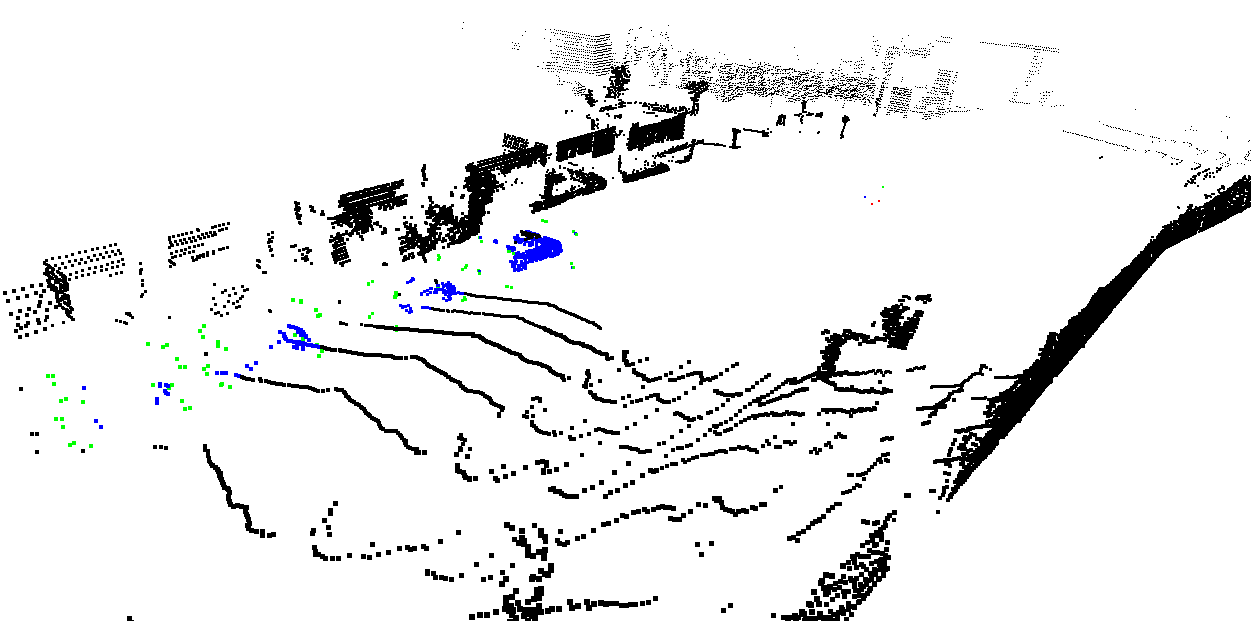
\includegraphics[height=2cm]{data/kitti/snapshot03_rect}};
    
    % https://tex.stackexchange.com/questions/40840/put-a-node-behind-another-in-a-tikz-diagram
    %\begin{scope}[on background layer]
    %  \node[] at (3,-1.5) {\includegraphics[width=5.5cm,trim={4cm 1cm 13cm 3cm},clip]{data/kitti/snapshot_00_rect_fade}};
    %\end{scope}
    
    %\node[rectangle,draw=black] at (-0.9,-2.75) {\includegraphics[height=2cm]{data/shapenet/simplification/1104f0924e03f2b6fc5886e868449015}};
    %\node[rectangle,draw=black] at (2.6,-2.75) {\includegraphics[height=2cm]{data/shapenet/simplification/1089cbe82dc0e72133d7c9e122eec9b6}};
    
    \node at (0, 1.5) {Mesh};
    \node[rectangle,draw=black,fill=white] (m) at (0,0) {
      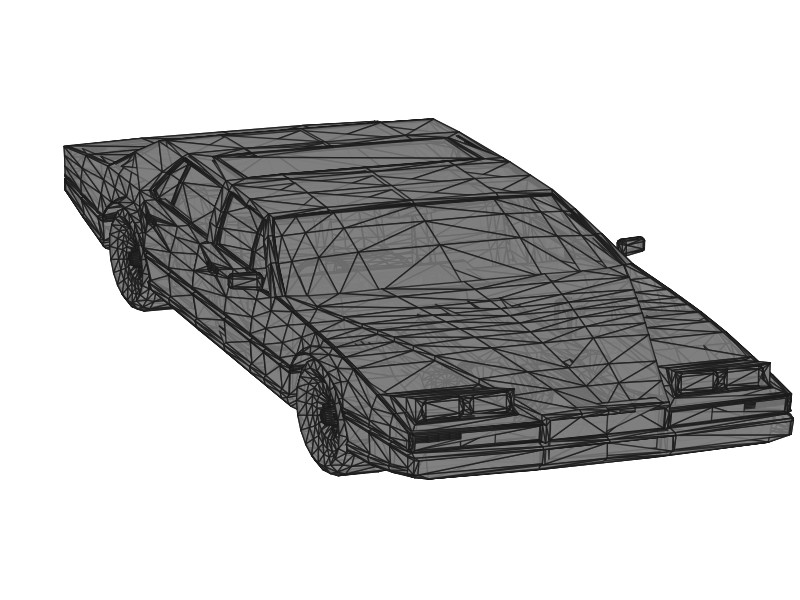
\includegraphics[height=2.25cm]{data/shapenet/dd84236f0ef27765a134736201a79843}
    };
    
    \node at (6, 1.5) {Simplified Mesh};
    \node[rectangle,draw=black,fill=white] (s) at (6,0) {
      
\includegraphics[height=2.25cm,trim={1cm 1cm 1cm 1cm},clip]{data/shapenet/0}
    };
    
    \node at (12, 1.5) {Occupancy Grid};
    \node[rectangle,draw=black,fill=white] (o) at (12,0) {
      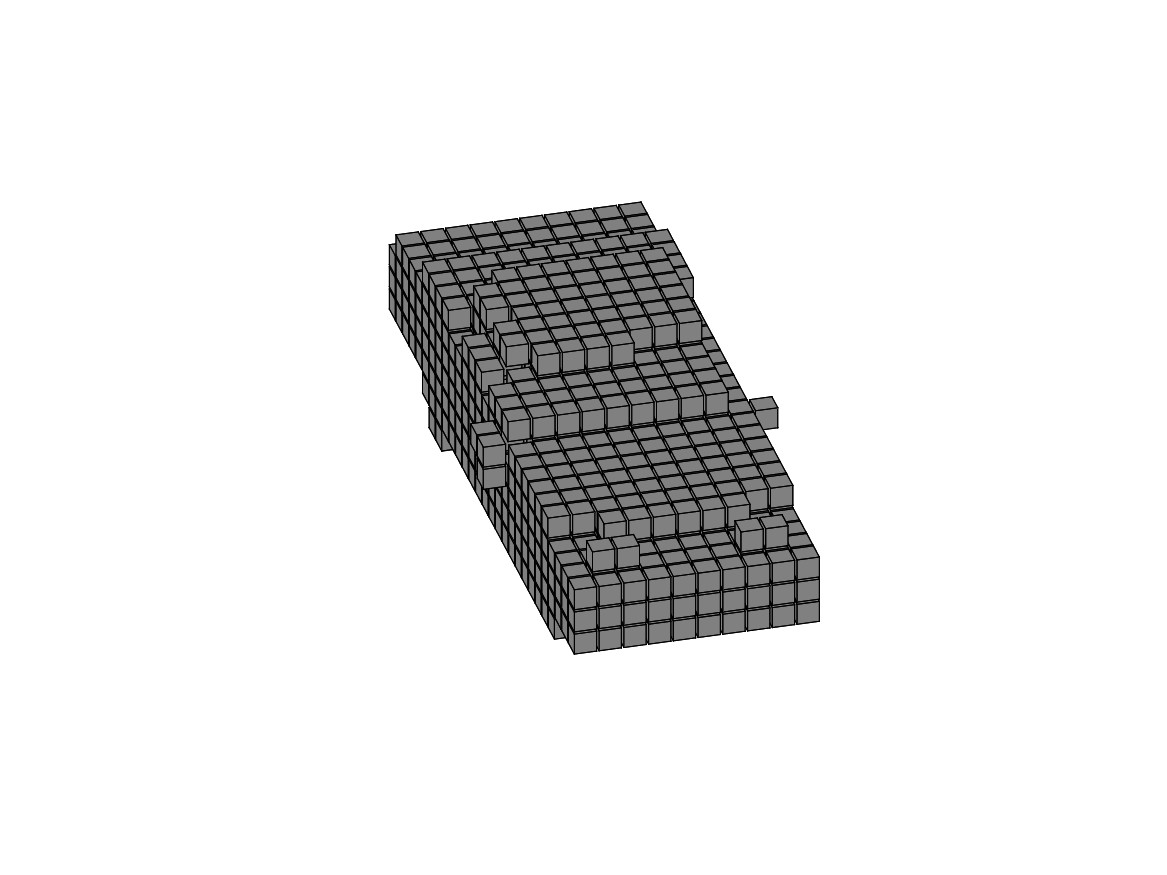
\includegraphics[height=2.25cm,trim={3cm 2cm 3cm 2cm},clip]{data/shapenet/1_output_75}
    };
    
    \node at (3, 0.4) {\small Simplification};
    \node at (9, 0.4) {\small Voxelization};
    \draw[->] (m) -- (s);
    \draw[->] (s) -- (o);
    
    \node at (3.05, -3.75) {Signed Distance Function};
    \node[rectangle,draw=black,fill=white] (sdf) at (3.05,-2.5) {
      \begin{tabular}{@{}c@{}}
        
\includegraphics[width=8.4cm]{data/shapenet/1_sdf_output_slices}\\[-6px]
        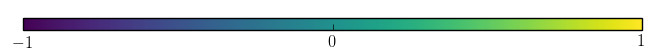
\includegraphics[width=9.05cm]{data/shapenet/sdf_colorbar}
      \end{tabular}
    };
    
    \node at (10, -3) {Distance Transform};
    \draw[-,dashed] (o) -- (12, -2.5);
    \draw[->,dashed] (12,-2.5) -- (sdf);
  \end{tikzpicture}
  \vskip 6px
  
  % TODO short caption
  \caption{Illustration of the used modalities, \ie occupancy grids and
  signed distance functions. In particular, a given triangular mesh is first
  simplified in order to reduce its complexity and obtain a watertight mesh
  which is required for voxelization, \ie to obtain an occupancy grid.
  In this thesis, we derive the corresponding signed distance function from the occupancy
  grid using a distance transform -- as illustrated by the dashed line. We note,
  however, that signed distance functions should in general be derived from
  the original mesh in order to obtain sub-voxel accuracy.}
  \label{fig:shape-representation}
\end{figure}

\section{Meshes}

Another source of information for our problem are datasets
of Computer-Aided Design (CAD) models. In this thesis, we assume that
CAD models are provided as triangular meshes -- we refer to
\cite{BotschKobbelt:2010} for a detailed introduction.
Regarding Problem \ref{problem},
these correspond to a raw version of the shape set $\mathcal{Y}$:

% TODO computation graph mathcal
% TODO wording and \mathcal{M} everywhere
\begin{definition}
  A triangular mesh $\mathcal{M} = (V, F)$ is defined by a set of 
  vertices $V \subseteq \mathbb{R}^3$ and a set of triangular faces
  $F \subseteq \{1,\ldots,|V|\}^3$ such that $f = (f_1, f_2, f_3) \in F$
  defines a triangular face enclosed by the corresponding vertices
  $v_{f_1}$, $v_{f_2}$ and $v_{f_3}$. Faces implicitly also define the edges
  $E(F)$ between the vertices.
\end{definition}

An illustration of a triangular mesh from ShapeNet can be found in Figure
\ref{fig:shape-representation}. The concepts of adjacency and incidency
are naturally extended to triangular meshes. We note that a triangular mesh
only defines the surface of an object. Without additional constraints it is
generally hard to reason about the interior and exterior of the surface
-- and whether the surface is closed.
As we also see in Chapter \ref{ch:data}, this question naturally leads to the
concept of watertight meshes. In the literature \cite[Section~1.3]{BotschKobbelt:2010},
watertight meshes are usually defined as 2-manifold meshes without boundary edges,
see Appendix \ref{ch:appendix-shape-representation} for details.
Another problem, illustrated in Figure \ref{fig:shape-representation}, concerns
very detailed meshes, \ie meshes consisting of a
large number of faces and vertices, often going into the tenth of thousands. 
Therefore, mesh simplification \cite[Chapter~6]{BotschKobbelt:2010} is an important
problem in computer graphics. In Chapter \ref{ch:data} we will present a very
practical approach to compute very rough, simplified meshes. In our case, this algorithm
solves both problems -- obtaining watertight and simplified meshes.

\section{Occupancy Grids}
\label{sec:shape-representation-occupancy}

Given point clouds or watertight meshes, occupancy grids are a natural representation
for applying deep learning techniques. In particular, 3D convolutional neural networks
are able to operate directly on the provided topology and thereby
utilize spatial information. Operating
directly on triangular meshes or point clouds, in contrast, is less straight-forward
regarding a proper representation (\eg for encoding the faces) which would need
to be invariant to the order of faces or points \cite{GarciaGarciaLopez:2016,FanSuGuibas:2016}
and allow to leverage local information
\cite{QiYiSuGuibas:2017,GuoChen:2015,BoscainiVandergheynst:2015,BrunaLeCun:2013}.
Occupancy grids assume a voxelization of the space and
determine, for each voxel, its occupancy. Specifically, a voxel is
considered occupied if it lies inside the interior of the shape or intersects with
its surface. For point clouds, a voxel is considered occupied if it contains at
least one point.

\begin{definition}
  An occupancy grid is a tensor $x \in \{0,1\}^{H \times W \times D}$ where
  the elements $x_i$ are called voxels and $x_i = 1$ corresponds to an occupied
  voxel and $x_i = 0$ determines an unoccupied voxel.
\end{definition}

Occupancy grids can be interpreted as explicit shape representation. With
$H$, $W$ and $D$ being large enough, \ie using high resolution, even small details
of shapes can be captured, \eg see \cite{TatarchenkoBrox:2017}. In Figure
\ref{fig:shape-representation}, we illustrate the voxelization of the shown
simplified mesh.

\section{Signed Distance Functions}
\label{sec:shape-representation-sdf}

In contrast to occupancy grids, signed distance functions are used to define shapes
implicitly.
%Even in the computer graphics literature, where meshes are
%considered parametric representations, signed distance functions are described as
%implicit representation.
In the general case, a signed distance function
can be defined as follows \cite[Chapter~1]{BotschKobbelt:2010}:

% TODO wording and F
\begin{definition}
  Let $F:\mathbb{R}^3 \mapsto \mathbb{R}$ be a continuous function. Then,
  the surface of a shape is implicitly defined by the zero level-set
  $S := \{x \in \mathbb{R}^3 | F(x) = 0\}$ of $F$. As convention, $F$ is negative
  in the interior of the shape and positive in the exterior of the shape.
\end{definition}

%We consider continuous functions only, as we do not want shapes with holes.
The implicit representation through distance functions simplifies the problem
of determining the interior and exterior of a shape. The name stems from the
fact that $F$ is usually taken to be the signed distance to the nearest point
on the surface, \eg
\begin{align}
  |F(x)| = \min_{x_S \in S} \|x - x_S\|_2.
\end{align}
In order to numerically work with signed distance functions, they are usually
defined on a regular grid:

% TODO wording
\begin{definition}
  A signed distance function is a tensor $x \in \mathbb{R}^{H \times W \times D}$
  such that $x_i$ is the signed distance of the center of the corresponding voxel
  to the surface of the shape. It is negative inside the shape, and positive
  outside of it.
\end{definition}

% TODO cite marching cubes
In practice, and as simplification, we are computing signed distance functions
from occupancy grids. This is an important distinction; by using the
occupancy grid representation, we lose accuracy depending
on the used resolution. To re-gain higher accuracy, we could instead utilize a
signed distance function obtained from the original surface
\cite{LorensenCline:1987,BotschKobbelt:2010}; we leave this for future work.

\begin{remark}
  \label{rem:shape-representation-distance-function}
  Given an occupancy grid $x \in \{0,1\}^{H \times W \times D}$, we
  derive the corresponding distance function
  $\text{df}(x) \in \mathbb{R}^{H \times W \times D}$ as
  \begin{align}
    \text{df}_i(x) = \min_{j, x_j = 1} \|i - j\|_2.
  \end{align}
  Similarly, the signed distance function $\text{sdf}(x)$ can be
  defined by combining $\text{df}(x)$ and $\text{df}(1 - x)$
  with the appropriate signs.
\end{remark}

In practice, the conversion from occupancy grids to (signed) distance
functions can be computed using generalized distance transforms
\cite{FelzenswalbHuttenlocher:2012}. To compute the sign,
the interior and exterior must be known; for watertight meshes
the interior and exterior can be determined using occupancy grids
and connected components/flood filling algorithms \cite[Section~3.4]{Szeliski:2011}.
As defined above, we assume the distance function
$\text{df}_i(x)$ to represent the distance to the next occupied voxel $x_j = 1$
such that $\text{df}_i(1 - x)$ is the distance to the next unoccupied voxel.
We also found that using the log signed distance function, \ie
\begin{align}
  \text{lsdf}(x)_i = \sign(\text{sdf}(x)_i) \ln(1 + |\text{sdf}(x)_i|),
\end{align}
aids neural network training -- a strategy also employed for similar representations,
\eg for depth prediction \cite{EigenFergus:2015,EigenFergus:2014,LainaRupprechtNavab:2016}.
Intuitively, the log reduces the range of the prediction problem; in contrast to simple scaling,
however, the range is reduced non-linearly such that the range of small distances (\ie around
the zero level set) is effectively increased at the expense of larger distances.


% TODO remark?
%\begin{remark}
%  Given a signed distance function $\text{sdf}(x) \in \mathbb{R}^{H \times W \times D}$,
%  the log signed distance function is given by
%  \begin{align}
%    \text{lsdf}(x)_i = \sign(\text{sdf}(x)_i) \ln |\text{sdf}(x)_i|.
%  \end{align}
%\end{remark}

  \chapter{Shape Prior}
\label{ch:shape-prior}

\begin{figure}
  \begin{subfigure}[t]{0.48\textwidth}
    \centering
    \begin{tikzpicture}

      \node[rectangle,rounded corners=0.05cm,draw=black,minimum width=2cm,minimum height=3.5cm] (M) at (0.25, -1){};
      \node[above left] at (M.south east){$M$};
      \node[circle,draw=black,minimum size=1cm] (z) at (0,0){$z$};
      \node[circle,draw=black,minimum size=1cm] (y) at (0,-2){$y$};
      \node[] (w) at (-2,0){$w$};
      
      \draw[->] (w) -- (z);
      \draw[->] (y) -- (z);
      
    \end{tikzpicture}
    \vskip 6px
    \caption{A graphical model illustration of the recognition model $q(z|y)$, \ie
    the encoder. Here, the parameters $w$ are used to model $q(z|y)$ using a neural network.}
    \label{subfig:shape-prior-encoder}
  \end{subfigure}\hfill
  \begin{subfigure}[t]{0.48\textwidth}
    \centering
    \begin{tikzpicture}

      \node[rectangle,rounded corners=0.05cm,draw=black,minimum width=2cm,minimum height=3.5cm] (M) at (0.25, -1){};
      \node[above left] at (M.south east){$M$};
      \node[circle,draw=black,minimum size=1cm] (z) at (0,0){$z$};
      \node[circle,draw=black,minimum size=1cm] (y) at (0,-2){$y$};
      \node[] (w) at (2,0){$w$};
      
      \draw[->] (w) -- (z);
      \draw[->] (w) -- (y);
      \draw[->] (z) -- (y);

    \end{tikzpicture}
    \vskip 6px
    \caption{An illustration of the generative model $p(y|z)$, \ie the decoder
    which is modeled using a neural network and parameters $w$.}
    \label{subfig:shape-prior-latent-decoder}
  \end{subfigure}
  \vskip 6px
  % TODO short caption
  \caption[]{Illustration of the graphical models corresponding to encoder and decoder,
  \ie recognition model $q(z|y)$ and generative model $p(y|z)$.}
  \label{fig:shape-prior}
\end{figure}

Given occupancy grids or signed distance functions of
the shape set $\mathcal{Y}$ and the observations $\mathcal{X}$,
our approach to Problem \ref{problem} involves two steps:
first, we learn a shape prior defining the space of allowed shapes;
and second, we learn an inference model to embed the observations
within the same latent shape space.
The shape prior defines a joint distribution $p(y, z) = p(y | z) p(z)$
of shapes $y$ and latent codes~$z$. Essentially, the shape prior
represents an embedding of the shapes $\mathcal{Y}$
within a low-dimensional latent space~$\mathcal{Z}$. By enforcing a 
prior $p(z)$ on the latent space, we are able to generate shapes
using $y \sim p(y|z)$ for $z \sim p(z)$. Additionally, shape completion
can be defined over the low-dimensional latent space by also learning
an embedding $x \mapsto z$ of observations $x$ within the latent space.
In our formulation of amortized maximum likelihood, this embedding is deterministic.
For the proposed extended variational auto-encoder, the embedding is also probabilistic,
\ie expressed as $q(z | x)$.

In the following, we intend to learn the shape prior
using variational auto-encoders on set of shapes $\mathcal{Y} = \{y_1, \ldots, y_M\}$.
For occupancy grids or signed distance functions, we assume a flattened version
$y \in \mathbb{R}^R \simeq \mathbb{R}^{H \times W \times D}$ for simplicity.
The latent space is then given as $\mathcal{Z} = \mathbb{R}^Q$ for 
small $Q \ll R$.
A variational auto-encoder is an implementation of the more general
continuous latent variable model, which can easily be summarized using
the two graphical models in Figure~\ref{fig:shape-prior}. Although we are
mainly interested in the generative model $p(y | z)$ given a fixed prior $p(z)$,
training also requires learning the recognition model $q(z | y)$
in order to maximize the overall likelihood $p(y)$. For simple Gaussian models,
the recognition model $q(z | y)$ as well as the so-called marginal likelihood
\begin{align}
  p(y) = \int p(y, z) dz = \int p(y | z)p(z) dz
  \label{eq:shape-prior-marginal-likelihood}
\end{align}
can usually be determined analytically,
\eg see the discussion of probabilistic principal component analysis in
Appendix \ref{ch:appendix-shape-prior}. In the case of variational auto-encoders,
both the generative and the recognition model are implemented using neural networks.
Then, the recognition model as well as the marginal likelihood can only be approximated
-- mainly because the integral in Equation \eqref{eq:shape-prior-marginal-likelihood}
becomes intractable. In this chapter, we first follow \cite{BleiKucukelbirMcAuliffe:2016}
and \cite{Doersch:2016}
to introduce the framework of variational inference which allows to maximize a
lower bound on the likelihood. Subsequently, we discuss two variants of variational
auto-encoders where the prior $p(z)$ is either modeled using Gaussian distributions
or based on Bernoulli distributions -- corresponding to continuous latent variables
or binary latent variables, respectively.

\section{Variational Inference}
\label{sec:variational-inference}

In general, variational inference is posed as the problem of
finding a model distribution $q(z)$ to approximate 
the true posterior $p(z | y)$
\begin{align}
  q(z) = \argmin_{q} \KL(q(z) | p(z | y))\label{eq:shape-prior-variational-inference}
\end{align}
where the Kullback-Leibler divergence $\KL$ is a distance measure defined
on probability distributions.
The Kullback-Leibler divergence can then be rewritten to obtain a
lower bound on the intractable marginal likelihood $p(y)$.
The Kullback-Leibler divergence is formally defined as
(see \cite[Section~A.1]{KollerFriedman:2009} or \cite[Section~1.6]{Bishop:2006}):

\begin{definition}
  The Kullback-Leibler divergence between two probability
  distributions $q(z)$ and $p(z|y)$ is defined as:
  \begin{align}
    \KL(q(z) | p(z|y)) = \mathbb{E}_{q(z)}\left[\ln\frac{q(z)}{p(z|y)}\right]
  \end{align}
  where $\mathbb{E}_{q(z)}$ denotes the expectation with respect to
  the distribution $q(z)$.
\end{definition}

%\begin{lemma}
%  For the Kullback-Leibler divergence as introduced above, it holds:
%  \begin{align}
%   \KL(q(z) | p(z|y)) \geq 0
%  \end{align}
%  and $\KL(q(z) | p(z|y))$ if and only if $q(z) = p(z|y)$ almost everywhere.
%\end{lemma}

%\begin{proof}
%  A proof can be found in \cite[Section~1.6]{Bishop:2006}.
%\end{proof}

% TODO formally introduce the expection value notation!
%Starting from the Kullback-Leibler divergence $\KL(q(z) | p(z|y))$ we follow
%\cite{BleiKucukelbirMcAuliffe:2016} to derive the evidence lower bound,
%a lower bound on the likelihood $p(y)$ to maximize as surrogate objective.
A close look at the Kullback-Leibler
divergence reveals that the optimization problem in Equation
\eqref{eq:shape-prior-variational-inference}
involves computing the marginal likelihood:
\begin{align}
  \KL(q(z) | p(z|y)) &= \mathbb{E}_{q(z)}\left[\ln\frac{q(z)}{p(z|y)}\right]\label{eq:shape-prior-variational-inference-kl}\\
   &= \mathbb{E}_{q(z)}[\ln q(z)] - \mathbb{E}_{q(z)}[\ln p(z|y)]\\
   &= \mathbb{E}_{q(z)}[\ln q(z)] - \mathbb{E}_{q(z)}[\ln p(z,y)] + \ln p(y).
\end{align}
Re-arranging left- and right-hand side leads to the evidence lower bound which is also
referred to as variational lower bound \cite{BleiKucukelbirMcAuliffe:2016}:
\begin{align}
  \ln p(y) &= \KL(q(z) | p(z|y)) - \mathbb{E}_{q(z)}[\ln q(z)] + \mathbb{E}_{q(z)}[\ln p(z,y)]\\
  &\geq - \mathbb{E}_{q(z)}[\ln q(z)] + \mathbb{E}_{q(z)}[\ln p(z,y)]\\
  &= - \mathbb{E}_{q(z)}[\ln q(z)] + \mathbb{E}_{q(z)}[\ln p(z)] + \mathbb{E}_{q(z)}[\ln p(y|z)]\\
  &= - \KL(q(z) | p(z)) + \mathbb{E}_{q(z)}[\ln p(y|z)]
\end{align}
The original problem of maximizing the intractable marginal likelihood $p(y)$ in Equation
\eqref{eq:shape-prior-marginal-likelihood} is then approximated
by maximizing the evidence lower bound which we formally define as:

\begin{definition}
  The variational lower bound or evidence lower bound derived from Problem
  \eqref{eq:shape-prior-variational-inference} is given by
  \begin{align}
    - \KL(q(z) | p(z)) + \mathbb{E}_{q(z)}[\ln p(y|z)]
    = \mathbb{E}_{q(z)}\left[\ln\frac{p(y, z)}{q(z)}\right]
    \label{eq:shape-prior-variational-lower-bound}
  \end{align}
\end{definition}

In this general formulation of the evidence lower bound, the model distribution
$q(z)$ can be arbitrary. However, in the context of latent variable models,
it makes sense to make the model distribution depend on $y$ explicitly, \ie $q(z | y)$,
as we want to be able to reconstruct any $y$ from the corresponding latent code $z$.
Then, the evidence lower bound in Equation \eqref{eq:shape-prior-variational-lower-bound}
takes the form of an auto-encoder where
$q(z | y)$ represents the encoder and $p(y | z)$ the decoder.
Thus, a variational auto-encoder can be trained by maximizing the right-hand-side
of Equation \eqref{eq:shape-prior-variational-lower-bound}
after choosing suitable parameterizations for the distributions $p(z)$ and $q(z | y)$.
In the following, we first discuss the Gaussian case.

\section{Gaussian Variational Auto-Encoder}
\label{sec:shape-prior-gaussian-vae}

% TODO distributions in figure
In the framework of variational auto-encoders
\cite{KingmaWelling:2013}, the model
distribution $q(z|y)$ is implemented as neural network; similarly,
$p(y|z)$ is modeled as neural network.
%As in
%Example \ref{ex:deep-learning-convolutional-auto-encoder},
%the recognition model $q(z|y)$ is referred to as encoder;
%the generative network $p(y|z)$ is referred to as decoder.
In the case of Gaussian variational auto-encoders,
both $q(z|x)$ and $p(z)$ are assumed to be Gaussian, specifically
\begin{align}
  q(z|y) &= \mathcal{N}(z; \mu(y;w), \diag(\sigma^2(y;w)))\label{eq:recognition-model}\\
  p(z) &= \mathcal{N}(z; 0, I_Q)\label{eq:prior-model}
\end{align}
where the dependence on the neural network weights $w$
is made explicit; \ie both the mean $\mu(y;w) \in \mathbb{R}^Q$
and the covariance matrix
$\diag(\sigma^2(y;w)) \in\mathbb{R}^{Q \times Q}$
are predicted using a neural network with parameters $w$ that
are to be optimized.In the following we will neglect the weights $w$
for brevity.

% TODO Monte Carlo sampling
Considering the evidence lower bound from Equation
\eqref{eq:shape-prior-variational-lower-bound}, \ie
\begin{align}
  \eqref{eq:shape-prior-variational-lower-bound}
  = - \KL(q(z|y)|p(z)) + \mathbb{E}_{q(z|y)}[\ln p(y|z)],
\end{align}
the Kullback-Leibler divergence between $q(z|y)$
and $p(z)$ can be computed analytically. However, differentiating the lower
bound with respect to the hidden weights in $q(z|y)$ is problematic.
A classical Monte-Carlo approximation of the expectation $\mathbb{E}_{q(z|y)}[\ln p(y|z)]$
would require differentiating through the sampling process $z \sim q(z | y)$.
Therefore, Kingma and Welling \cite{KingmaWelling:2013} proposed
the so-called reparameterization trick. In particular,
the random variable $z \sim q(z|y)$ is reparameterized using a
differentiable transformation $g(z, \epsilon)$ based on an auxiliary
variable $\epsilon$ drawn from a unit Gaussian:
\begin{align}
	z_i = g_i(y, \epsilon_i) = \mu_i(y) + \epsilon_i \sigma_i^2(y)
\end{align}
with $\epsilon_i \sim \mathcal{N}(\epsilon; 0, 1)$.
Overall, given a sample
$y_m \in \mathbb{R}^R$, the objective to be minimized has the form
\begin{align}
	\mathcal{L}_{\text{VAE}} (w) = \KL(q(z|y_m) | p(z))
	- \frac{1}{L}\sum_{l = 1}^L \ln p(y_m | z_{l,m})\label{eq:shape-prior-variational-auto-encoder-objective}
\end{align}
where $z_{l,m} = g(\epsilon_{l,m}, y)$ and $\epsilon_{l,m} \sim \mathcal{N}(\epsilon ; 0, I_Q)$.
Here, $L$ is the number of samples to use for the Monte Carlo estimator of the
reconstruction error. In practice, the loss $\mathcal{L}_{\text{VAE}}$ is applied on
mini-batches and $L = 1$ is usually sufficient.

% TODO VAEs as ``verification''
Given the neural network weights $w$, the generation process can be
summarized as follows: draw $z \sim p(z) = \mathcal{N}(z ; 0,I_Q)$,
and draw $y \sim p(y|z)$. Similarly, recognition is performed by
drawing $z \sim q(z|y)$, \ie $\epsilon \sim \mathcal{N}(\epsilon ; 0,I_Q)$
and $z = g(y,\epsilon)$. For evaluation purposes, \ie for
measuring the recognition performance, $z$ is usually set to
$z = \mathbb{E}_{q(z|y)}[z]$; this can be accomplished
by directly considering $\mu(y)$.

\subsection{Practical Considerations}

% TODO log to ln
% TODO always upper bound for sums and products
As mentioned above, the Kullback-Leibler divergence of two Gaussian
distributions can easily be calculated directly.
As we consider diagonal covariance matrices the Kullback-Leibler divergence
is separable over $1 \leq i \leq Q$. Then, following \cite[Section~9]{Kullback:1959} 
(also see \cite[Appendix~A]{RasmussenWilliams:2006}) we have
\begin{align}
  \KL(\mathcal{N}(z_i ; \mu_{1,i}, \sigma_{1,i}^2)|\mathcal{N}(z_i ; \mu_{2,i},\sigma_{2,i}^2))
  = \frac{1}{2} \ln\frac{\sigma_{2,i}}{\sigma_{1,i}} + \frac{\sigma_{1,i}^2}{2\sigma_{2,i}^2} + \frac{(\mu_{1,i} - \mu_{2,i})^2}{2 \sigma_{2,i}^2} - \frac{1}{2}.
\end{align}
and with $\sigma_{2,i} = 1$ and $\mu_{2,i} = 0$
(and for simplicity $\sigma_i^2 := \sigma_i^2(y) = \sigma_{1,i}^2$ and $\mu_i := \mu_i(y) = \mu_{1,i} $) it follows:
\begin{align}
  \KL(p(z_i | y) | p(z_i)) = - \frac{1}{2} \ln \sigma_i + \frac{1}{2} \sigma_i^2 + \frac{1}{2} \mu_i^2 - \frac{1}{2}.
  %&= \KL(\mathcal{N}(z_i ; \mu_i, \sigma_i^2) | \mathcal{N}(z_i ; 0, 1))\\
  \label{eq:shape-prior-analyitcal-kld}
\end{align}
%In practice, letting the encoder predict $\sigma^2(y)$ directly is problematic
%as $\sigma^2(y)$ may not be negative. We can avoid this constraint by predicting
%log-variances instead, \ie $l_i(y) := \ln \sigma_i^2(y)$. Then, the Kullback-Leibler
%divergence from Equation \eqref{eq:shape-prior-analyitcal-kld} changes to
%\begin{align}
%  \KL(\mathcal{N}(y_i ; y_i, l_i) | \mathcal{N}(y_i ; 0, 0))
%  = -\frac{1}{2}l_i + \frac{1}{2} \exp(l_i) + \frac{1}{2} \mu_i^2 - \frac{1}{2}
%\end{align}
%and the reparameterization trick can be written as
%\begin{align}
%  z_i = g(y, \epsilon_i) = \mu_i + \epsilon_i \exp\left(\frac{1}{2}l_i\right).
%\end{align}

% TODO losses parameters
The remaining part of the objective
is the reconstruction error, \ie the negative log-likelihood $- \ln p(y | z_l)$.
This depends on how $p(y|z)$ is modeled; in our case, $p(y|z)$
is decomposed element-wise over voxels:
\begin{align}
  p(y|z) = \prod_{i = 1}^R p(y_i | z)\quad\Rightarrow\quad -\ln p(y | z) = -\sum_{i = 1}^R \ln p(y_i | z)
\end{align}
For shapes $y$ in the form of occupancy grids, we use Bernoulli distributions
to model individual voxels, \ie $p(y_i | z) = \Ber(y_i ; \theta_i(z))$ where
the probabilities of occupancy $\theta_i(z)$ are predicted using the decoder.
The negative log-likelihood then 
reduces to the binary cross entropy error. When working with signed distance functions,
we use Gaussian distributions with fixed variance to model individual voxels,
\ie $p(y_i | z) = \mathcal{N}(y_i; \mu_i(z), \sigma^2)$ where the $\mu_i(z)$'s
are predicted by the decoder. In this case, the negative log-likelihood leads
to the sum-of-squared error. See Section \ref{sec:deep-learning-losses} for details.

For illustration and implementation purposes, we define two additional layers:

% TODO indicate Gaussian
\begin{definition}
  \label{def:shape-prior-kld-layer}
  A Gaussian Kullback-Leibler divergence layer $\text{KLD}_{\mathcal{N}}$
  takes as input two tensors $\mu \in \mathbb{R}^{B \times Q}$ and
  $\sigma^2 \in \mathbb{R}^{B \times Q}$ and computes the Kullback-Leibler
  divergence
  \begin{align}
    \sum_{b = 1}^B \KL(\mathcal{N}(z;\mu_b,\diag(\sigma_b^2)) | \mathcal{N}(z;0,I_Q)),
  \end{align}
  before passing the predicted $\mu_b, \sigma_b^2 \in \mathbb{R}^Q$
  on to the next layer (unchanged):
  \begin{align}
    \text{KLD}_{\mathcal{N}}(\mu, \sigma^2) = (\mu, \sigma^2).
  \end{align}
\end{definition}

% TODO write it exactly!
Essentially, this layer just makes the computation of the Kullback-Leibler
divergence explicit -- in a separate layer. This means that the forward pass
is unaffected. However, it is important to consider the derivatives
with respect to the predicted $\mu(y)$ and $\sigma^2(y)$ as these
need to be added to the decoder's gradients (coming from the reconstruction loss)
during error backpropagation in order to account for the Kullback-Leibler divergence
during training:
\begin{align}
  \frac{\partial \KL(p(z_i|y) | p(z_i))}{\partial \mu_i} = \mu_i
  \quad\text{ and }\quad
  \frac{\partial \KL(p(z_i|y) | p(z_i))}{\partial \sigma_i} = - \frac{1}{2\sigma_i} + \sigma_i
  %\quad\Leftrightarrow\quad \frac{\partial \KL(\mathcal{N}(y_i ; \sigma_i, l_i) | \mathcal{N}(y_i; 0, 0)}{\partial l_i}
  %= - \frac{1}{2} + \frac{1}{2} \exp(l_i).
\end{align}
After computing the Kullback-Leibler divergence, the reparameterization trick
is applied:

% TODO notation of epsilon and dimensions
\begin{definition}
  \label{def:shape-prior-repa-layer}
  A Gaussian reparameterization layer $\text{repa}_{\mathcal{N}}$
  takes as input two tensors $\mu \in \mathbb{R}^{B \times Q}$ and
  $\sigma^2 \in \mathbb{R}^{B \times Q}$ and computes a single output
  tensor
  \begin{align}
    \text{repa}_{\mathcal{N}}(\mu, \sigma^2) = \mu + \epsilon \sigma
    \label{eq:shape-prior-repa-layer}
  \end{align}
  where $\epsilon \in \mathbb{R}^{B \times Q}$,
  $\epsilon_{b,i} \sim \mathcal{N}(\epsilon;0,1)$, and $\mu$ are multiplied
  element-wise.
\end{definition}

Again, we note that the primary purpose of the reparameterization layer is
to sample from $q(z | y)$ in a differentiable manner. Then, the following example
illustrates how a convolutional auto-encoder such
as the one from Example \ref{ex:deep-learning-convolutional-auto-encoder}
can be ``upgraded'' to a variational auto-encoder using the newly introduced
layers:

\begin{figure}
  \centering
  \hspace*{-0.75cm}
  \begin{tikzpicture}
    \node (y) at (0,0) {\small$y$};

    \node[conv,rotate=90,minimum width=4.5cm] (conv1) at (1.25,0) {\small$\text{conv}_{1, 16, 3}$\,+\,$\text{bn}$\,+\,$\ReLU$};
    \node[pool,rotate=90,minimum width=4.5cm] (pool1) at (2.5,0) {\small$\text{pool}_{2}$};
    \node[conv,rotate=90,minimum width=4.5cm] (conv2) at (3.75,0) {\small$\text{conv}_{16, 32, 3}$\,+\,$\text{bn}$\,+\,$\ReLU$};
    \node[pool,rotate=90,minimum width=4.5cm] (pool2) at (5,0) {\small$\text{pool}_{2}$};
    \node[conv,rotate=90,minimum width=4.5cm] (conv3) at (6.25,0) {\small$\text{conv}_{32, 64, 3}$\,+\,$\text{bn}$\,+\,$\ReLU$};
    \node[pool,rotate=90,minimum width=4.5cm] (pool3) at (7.5,0) {\small$\text{pool}_{2}$};
    \node[conv,rotate=90,minimum width=4.5cm] (conv4) at (8.75,0) {\small$\text{conv}_{64, 128, 3}$\,+\,$\text{bn}$\,+\,$\ReLU$};
    \node[pool,rotate=90,minimum width=4.5cm] (pool4) at (10,0) {\small$\text{pool}_{2}$};
    
    \node[view,rotate=90,minimum width=4.5cm] (view4) at (11.25,0) {\small$\text{view}_{B, 1024}$};
    
    \node[fc,rotate=90, minimum width = 2cm] (fc51) at (12.5,1.25) {\small$\text{fc}_{512, Q}$};
    \node[fc,rotate=90, minimum width = 2cm] (fc52) at (12.5,-1.25) {\small$\text{fc}_{512, Q}$};
  
    \node[view,rotate=90,minimum width=4.5cm] (kld) at (13.75,0) {\small$\text{KLD}_{\mathcal{N}}$\,+\,$\text{repa}_{\mathcal{N}}$};
    
    \node (z) at (13.75,-5){\small$\tilde{z}$};
    
    \node[fc,rotate=90,minimum width=4.5cm] (fc6) at (12.5,-5) {\small$\text{fc}_{Q, 512}$};
    \node[view,rotate=90,minimum width=4.5cm] (view6) at (11.25,-5) {\small$\text{view}_{B, 1024, 2, 2, 2}$};
    
    \node[up,rotate=90,minimum width=4.5cm] (up7) at (10,-5) {\small$\text{nnup}_{2}$};
    \node[conv,rotate=90,minimum width=4.5cm] (conv7) at (8.75,-5) {\small$\text{conv}_{128, 64, 3}$\,+\,$\text{bn}$\,+\,$\ReLU$};
    \node[up,rotate=90,minimum width=4.5cm] (up8) at (7.5,-5) {\small$\text{nnup}_{2}$};
    \node[conv,rotate=90,minimum width=4.5cm] (conv8) at (6.25,-5) {\small$\text{conv}_{64, 32, 3}$\,+\,$\text{bn}$\,+\,$\ReLU$};
    \node[up,rotate=90,minimum width=4.5cm] (up9) at (5,-5) {\small$\text{nnup}_{2}$};
    \node[conv,rotate=90,minimum width=4.5cm] (conv9) at (3.75,-5) {\small$\text{conv}_{32, 16, 3}$\,+\,$\text{bn}$\,+\,$\ReLU$};
    \node[up,rotate=90,minimum width=4.5cm] (up10) at (2.5,-5) {\small$\text{nnup}_{2}$};
    \node[conv,rotate=90,minimum width=4.5cm] (conv10) at (1.25,-5) {\small$\text{conv}_{16, 1, 3}$\,+\,$\text{bn}$\,+\,$h$};
    
    \node (ry) at (0,-5) {\small$\tilde{y}$};
    
    \draw[->] (y) -- (conv1);
    \draw[->] (conv1) -- (pool1);
    \draw[->] (pool1) -- (conv2);
    
    \draw[->] (conv2) -- (pool2);
    \draw[->] (pool2) -- (conv3);
    
    \draw[->] (conv3) -- (pool3);
    \draw[->] (pool3) -- (conv4);
    
    \draw[->] (conv4) -- (pool4);
    \draw[->] (pool4) -- (view4);
    
    \draw[->] (view4) -- (fc51);
    \draw[->] (view4) -- (fc52);
    
    \draw[->] (fc51) -- (kld);
    \draw[->] (fc52) -- (kld);
    
    \draw[->] (kld) -- (z);
    \draw[->] (z) -- (fc6);
    \draw[->] (fc6) -- (view6);
    
    \draw[->] (view6) -- (up7);
    \draw[->] (up7) -- (conv7);
    
    \draw[->] (conv7) -- (up8);
    \draw[->] (up8) -- (conv8);
    
    \draw[->] (conv8) -- (up9);
    \draw[->] (up9) -- (conv9);
    
    \draw[->] (conv9) -- (up10);
    \draw[->] (up10) -- (conv10);
    
    \draw[->] (conv10) -- (ry);

    \node[rotate=90] (L) at (0, -2.5) {\small$\mathcal{L}(\tilde{y}, y) = -\ln p(y | \tilde{z})$};
    \draw[-,dashed] (y) -- (L);
    \draw[-,dashed] (ry) -- (L);

    \node[rotate=90] (KLD) at (14.5, -5) {\small$\KL(q(z|y) | p(z))$};
    \draw[-,dashed] (KLD) -- (z);
  \end{tikzpicture}
  \vskip 6px
  \caption{An illustration of a Gaussian variational auto-encoder with
  four convolutional stages in both encoder and decoder. This is also the
  architecture used in experiments in Chapter \ref{ch:experiments} where
  we assume volumes of size
  $32 \times 32 \times 32$ such that the spatial size just before
  the fully connected layers of the encoder is $2 \times 2 \times 2$
  resulting in a $1024$-dimensional representation when considering $128$
  channels. See Example \ref{ex:shape-prior-variational-auto-encoder} for details.}
  \label{subfig:experiments-2d-architecture-vae}
\end{figure}

\begin{example}
  \label{ex:shape-prior-variational-auto-encoder}
  We consider Figure \ref{subfig:experiments-2d-architecture-vae} of our
  implementation of a variational auto-encoder with four convolutional
  stages in the encoder and decoder. In the case of the encoder, two fully connected layers
  independently compute the mean $\mu(y) \in \mathbb{R}^Q$ and variance
  $\sigma^2(y) \in \mathbb{R}^Q$ given the same input. Then, the Kullback-Leibler
  divergence $\KL(q(z|y) |p(z))$
  is computed and mean and variance are passed into the reparameterization
  layer. Here, an auxiliary variable $\epsilon \sim \mathcal{N}(\epsilon; 0, I_Q))$
  is chosen in order to sample a latent code $z \sim q(z| y) = \mathcal{N}(z;\mu(y),\diag(\sigma^2(y)))$
  using $z = g(y, \epsilon)$ and then passed into the decoder.
  At test time, the reparameterization layer can be removed, and the predicted
  mean $\mu(y)$ can be directly passed into the decoder. In the illustration,
  we also make the reconstruction loss $\mathcal{L}(\tilde{y}, y) = -\ln p(y | \tilde{z})$
  explicit.
\end{example}
% TODO layers, example, figure

In practice, letting the encoder predict $\sigma^2(y)$ directly is problematic
as the variance $\sigma^2(y)$ may not be negative. Therefore, we follow
publicly available implementations\footnote{
  For example \url{https://github.com/y0ast/VAE-Torch}, \url{https://github.com/staturecrane/dcgan_vae_torch} and \url{https://github.com/Kaixhin/Autoencoders}.
}
and let the encoder predict log-variances instead, \ie $l_i (y) := \ln \sigma^2(y)$.
This makes sure that the variance $\sigma^2(y) = \exp(l_i (y))$ will always be
positive. The Kullback-Leibler divergence from Equation 
\eqref{eq:shape-prior-analyitcal-kld} and the corresponding derivative with
respect to $l_i (y)$ as well as the reparameterization trick from Equation
\eqref{eq:shape-prior-repa-layer} are easily adapted.

Training a Gaussian variational auto-encoder in practice means
balancing the -- possibly conflicting -- objectives corresponding to
reconstruction loss and Kullback-Leibler divergence.
While the reconstruction loss is intuitively interpretable, \eg as binary cross
entropy error or scaled sum-of-squared error in the Bernoulli and Gaussian
cases, respectively, the Kullback-Leibler divergence is less intuitive.
Therefore, it might be beneficial to monitor
the latent space statistics over a held-out validation set. Concretely, this means
monitoring the first two moments of the predicted means, \ie
\begin{align}
  \overline{\mu} = \frac{1}{QM'} \sum_{i = 1}^Q\sum_{m = 1}^{M'} \mu_i(y_m)
  \label{eq:shape-prior-monitor-mean-mean}
\end{align}
and
\begin{align}
  \Var[\mu] = \frac{1}{QM'}\sum_{i = 1}^Q\sum_{m = 1}^{M'} (\mu_i(y_m) - \overline{\mu})^2
  \label{eq:shape-prior-monitor-variance-mean}
\end{align}
where $M'$ is the size of the validation set. Additionally, it is worth
monitoring the first moment of the predicted log-variances
\begin{align}
  \overline{l} = \frac{1}{QM'} \sum_{i = 1}^Q\sum_{m = 1}^{M'} \ln \sigma_i^2(y_m) = \frac{1}{QM'} \sum_{i = 1}^Q\sum_{m = 1}^{M'} l_i(y_m).
  \label{eq:shape-prior-monitor-mean-variance}
\end{align}
Note that these statistics are computed over all $Q$ dimensions of the latent
space -- this is appropriate as the prior $p(z)$ is a unit Gaussian such that
all dimensions can be treated equally.
During training, these statistics should converge to a unit Gaussian,
\ie $\overline{\mu} \approx 0$ and $\Var[\mu] \approx 1$, and the network
should be capable of making certain predictions, \ie small $\overline{l}$.

\section{Bernoulli Variational Auto-Encoder}
\label{sec:shape-prior-bernoulli-vae}

The Gaussian variational auto-encoder will be used to learn the latent space~$\mathcal{Z}$,
\ie the shape prior. However, in the case of the extended variational
auto-encoder for shape completion we intend to model the joint
probability $p(x, y, z)$ by introducing random variables for the observations
$x_i$, as well. Here, both $y$ and $z$ are considered to be latent variables,
therefore, we also need to be able to model discrete latent variables -- particularly
binary latent variables considering $y$ to be represented as occupancy grid.
Unfortunately, this is not straight-forward in the framework presented so far.

Recently, however, researchers \cite{MaddisonMnihTeh:2016,JangGuPoole:2016}
were able to model both $p(z)$ and $q(z|y)$ using Bernoulli distributions,
\ie
\begin{align}
  p(z) &= \prod_{i = 1}^Q \Ber(z_i; 0.5)\\
  p(z | y) &= \prod_{i = 1}^Q \Ber(z_i; \theta_i(y))
\end{align}
where $\theta_i(y)$ are predicted using the encoder, given the input $y$.
Again, the evidence lower bound is to be optimized, this means for a sample $y_m$:
\begin{align}
  \mathcal{L}_{\text{VAE}} (w) = \KL(q(z|y_m) | p(z))
	- \frac{1}{L}\sum_{l = 1}^L \ln p(y_m | z_{l,m})
\end{align}
where $z_{l,m} \sim q(z|y)$. The Kullback-Leibler divergence can be
computed analytically, however, differentiation
through the sampling process $z_{l,m} \sim q(z | y)$
is problematic. Unfortunately, the reparameterization trick used in
the Gaussian case is not applicable anymore.
At this point, Maddison \etal \cite{MaddisonMnihTeh:2016} and, concurrently, Jang \etal
\cite{JangGuPoole:2016} propose an alternative reparameterization trick
for general discrete distributions which we define as follows:

\begin{definition}
  Let $z \in \{1,\ldots,K\}$ be a random variable; then $z$ is distributed
  according to a discrete distribution, \ie $z \sim \Dis(z; \pi)$,
  with parameters $\pi = (\pi_1, \ldots, \pi_K)$ if
  \begin{align}
    p(z = k) = \pi_k\quad\text{ and }\quad \sum_{k = 1}^K \pi_k = 1.
  \end{align}
  We represent $z$ using the so-called one-hot encoding, meaning that
  $z \in \{0,1\}^K$ such that $z_k = 1$ and $z_{k'} = 0$, $k' \neq k$
  if event $k$ occurs.
  %In the following we also assume $\pi_i > 0$ as categories
  %corresponding to $\pi_i = 0$ can be discarded.
\end{definition}

The reparameterization is additionally based on the Gumbel distribution:

% TODO Gu(e,mu,beta)?
\begin{definition}
  Let $\epsilon \in \mathbb{R}$ be a random variable. Then $\epsilon$
  is distributed according to the Gumbel distribution,
  \ie $\epsilon \sim \Gu(\epsilon; \mu, \beta)$,
  with parameters $\mu$ and $\beta$ if
  \begin{align}
    p(\epsilon) = \exp\left(- \exp\left(-\frac{\epsilon - \mu}{\beta}\right)\right).
  \end{align}
  The standard Gumbel distribution is
  the special case of $\mu = 0$ and $\beta = 1$.
\end{definition}

% TODO cite sampling
A key insight is that it is very easy to sample from a Gumbel distribution:
let $u_k \sim U(0,1)$, then $\epsilon_k = \mu - \beta \log(-\log(u_k))$
is distributed according to $\Gu(\mu, \beta)$. The standard Gumbel
distribution also helps to sample from a discrete distribution. Let 
$\epsilon_{1},\ldots,\epsilon_{K} \sim \Gu(\epsilon; 0, 1)$, then set $z_k = 1$ for
\begin{align}
  k = \argmax_{k} \ln \pi_k + \epsilon_{k}
  \label{eq:shape-prior-bernoulli-repa}
\end{align}
and $z$ will be distributed according to a discrete distribution, \ie $z \sim \Dis(z;\pi)$;
this is called the Gumbel trick.
Replacing the $\argmax$ with its smooth counterpart, \ie the softmax,
yields the final reparameterization trick:
\begin{align}
  z_k = \frac{\exp(\ln \pi_k + \epsilon_k)}{\sum_{k' = 1}^d \exp(\ln \pi_{k'} + \epsilon_{k'})}.
  \label{eq:shape-prior-discrete-repa}
\end{align}
Both Maddison \etal \cite{MaddisonMnihTeh:2016} and Jang \etal \cite{JangGuPoole:2016}
additionally add a temperature parameter, \ie $\frac{\ln \pi_k + \epsilon_k}{\lambda}$,
and show that for $\lambda \rightarrow 0$, Equation \eqref{eq:shape-prior-discrete-repa}
tends to the real discrete distribution. However, for simplicity, we neglect
the temperature $\lambda$ in our discussion.

The Bernoulli distribution is a special case of the discrete distribution.
Letting $z \sim \Ber(z;\theta)$, $z = 1$ means that
\begin{align}
  \ln \theta + \epsilon_1 > \ln (1 - \theta) + \epsilon_2
\end{align}
where we used Equation \eqref{eq:shape-prior-bernoulli-repa} with $\pi_1 = \theta$
being the probability of $z = 1$ and $\pi_2 = (1 - \theta)$ the probability of $z = 0$
and made the $\argmax$ explicit through the inequality.
Maddison \etal \cite{MaddisonMnihTeh:2016} argue that the difference
of two Gumbel random variables $\epsilon_1 - \epsilon_2$ is distributed according
to a Logistic distribution (also see \cite[Section~5]{BenAkivaLerman:1985}) where
we can sample from using
\begin{align}
  \epsilon_1 - \epsilon_2 = \ln u - \ln (1 - u)
\end{align}
with $u \sim U(0,1)$. Thus,
\begin{align}
  z = \begin{cases}
    1&\quad\ln u - \ln (1 - u) + \ln \theta - \ln (1 - \theta) > 0\\
    0&\quad\text{else}
  \end{cases}
\end{align}
which can be made differentiable using a soft thresholding operation
such as the sigmoid function.
With a change in notation, letting $\epsilon \sim U(0,1)$ this results in
\begin{align}
  z_i = g(y, \epsilon) = \sigma\left(\ln \epsilon - \ln (1 - \epsilon) + \ln \theta_i(y) - \ln (1 - \theta_i(y))\right)
  \label{eq:shape-prior-reparameterization-bernoulli}
\end{align}
which is the final reparameterization trick used. The remaining framework stays
unchanged; the Kullback-Leibler divergence is again computed analytically
and the reconstruction error $- \ln p(y | z)$ depends on the exact form
of $p(y |z)$ as discussed before.

% TODO analytical form of KLD
\subsection{Practical Considerations}
\label{sec:shape-prior-vae-practical-considerations}

The main difference between a Gaussian variational auto-encoder and
the Bernoulli counterpart is the reparameterization trick and the corresponding
Kullback-Leibler divergence. The latter can, again, be separated over $1 \leq i \leq Q$
and then be calculated analytically:
\begin{align}
  \KL(q(z_i | y) | p(z_i)) &= \KL(\Ber(z_i; \theta_i(y)) | \Ber(z_i; 0.5))\\
  %&= \KL(\Ber(z_i;\theta_i(y)) | \Ber(z_i;0.5))\\
  %&= \mathbb{E}_{\Ber(z_i;\theta_i(y))}\left[\ln\frac{\Ber(z_i;\theta_i(y))}{\Ber(z_i;0.5)}\right]\\
  &= \sum_{k \in \{0,1\}} \ln \theta_i(y)^k (1 - \theta_i(y))^{1 - k} - \ln 0.5^k 0.5^{1-k}
  \label{eq:shape-prior-bernoulli-kld}
\end{align}
where we use $\Ber(z_i;0.5)$ as prior, \ie our standard Bernoulli
distribution. The gradient with respect to the parameters $\theta_i(y)$
is, as before, added during error backpropagation. This leads to
the Bernoulli Kullback-Leibler divergence layer:

\begin{definition}
  \label{def:shape-prior-bernoulli-kld}
  A Bernoulli Kullback-Leibler divergence layer $\text{KLD}_{\Ber}$ takes as
  input a tensor $\theta \in \mathbb{R}^{B \times Q}$ and computes the Kullback-Leibler
  divergence
  \begin{align}
    \sum_{b = 1}^B \sum_{i = 1}^Q \KL(\Ber(z_{b,i}; \theta_{b,i}) |  \Ber(z_{b,i}; 0.5))
  \end{align}
  before passing the predicted $\theta$ on to the next layer (unchanged):
  \begin{align}
    \text{KLD}_{\Ber}(\theta) = \theta.
  \end{align}
\end{definition}

Again, this layer just makes the computation of the Kullback-Leibler
divergence explicit and takes care of adding the corresponding derivative
-- which is easily derived from Equation \eqref{eq:shape-prior-bernoulli-kld} --
during error backpropgation.
The reparameterization trick as outlined in Equation
\eqref{eq:shape-prior-reparameterization-bernoulli} is wrapped in the following
layer which needs to be followed by a sigmoid non-linearity layer
to have the desired effect:

\begin{definition}
  \label{def:shape-prior-bernoulli-repa}
  A Bernoulli reparameterization layer $\text{repa}_{\Ber}$ takes as
  input a tensor $\theta \in \mathbb{R}^{B \times Q}$ and computes
  \begin{align}
    \text{repa}_{\Ber}(\theta) = \ln \epsilon - \ln (1 - \epsilon)
    + \ln \theta -\ln (1 - \theta)
  \end{align}
  where $\epsilon \in \mathbb{R}^{B \times Q}$ with $\epsilon_i \sim U(0,1)$.
\end{definition}

The combination of both layers is analogous to the case of Gaussian
variational auto-encoder except that a logistic sigmoid
non-linearity layer needs to be added right after the reparameterization layer.

\section{Discussion}

Overall, we introduced variational
auto-encoders for continuous latent variables as well as binary
latent variables. In practice, variational auto-encoders
are very similar to standard auto-encoders except that encoder and decoder
predict probability distributions, \ie $q(z | x)$ and $p(y | x)$.
Additionally, the Kullback-Leibler divergence makes sure
that the encoder, \ie the recognition model $q(z | y)$, matches a pre-defined
prior $p(z)$. Then, the variational auto-encoder has the advantage of providing
a generative model, \ie $p(y | z)$. For shape completion, we use variational
auto-encoders to learn a shape prior allowing to easily constrain the space of
considered shapes. 

  \chapter{Shape Inference}
\label{ch:shape-inference}

So far, we are able to use the shape set
$\mathcal{Y} \subseteq \mathbb{R}^{H \times W \times D} \simeq \mathbb{R}^R$
from Problem \ref{problem} in order to learn a prior model $p(y,z)$ over a
possibly low dimensional latent space $\mathcal{Z} = \mathbb{R}^Q$. To this end,
we introduced variational auto-encoders where the generative model $p(y | z)$ and
the (approximate) recognition model $q(z | y)$ are implemented using
3D convolutional neural networks. In our first approach
to shape completion, we then intend to learn an inference model
\begin{align}
  x \mapsto \tilde{z} \approx &\argmax_{z} p(y = x | z) p(z)\label{eq:shape-inference-amortized-ml}
\end{align}
using a dataset of observations $x \in \mathbb{R}^{H \times W \times D}$.
We call this approach amortized maximum likelihood because we do not consider
the observations $x$ independently, but understand the maximum likelihood objective
as loss allowing to learn the deterministic embedding $x \mapsto \tilde{z}$ in an unsupervised
setting. Given the prior variational auto-encoder, this results in training a
new encoder while keeping the pre-trained decoder fixed.

In the proposed extended variational auto-encoder, we instead understand the
observation $x$ as a random variable. For the corresponding joint distribution
$p(x, y, z)$, we are able to derive the evidence lower bound assuming that
$y$ and $z$ are statistically independent given $x$. Similar to the shape prior,
we learn an approximate recognition model $q(z | x)$ which can be understood
as probabilistic embedding $x \mapsto z$. In contrast to amortized maximum likelihood,
the actual objective tying the observations $x$ to the shapes $y$ is
hidden in a Kullback-Leibler divergence. Again, the model can be trained
in an unsupervised fashion. In addition to training a new encoder, the
extended variational auto-encoder also implements an observation model $p(x | y)$ using a 
3D convolutional neural network. Compared to amortized maximum likelihood,
this potentially allows to explicitly integrate knowledge about the observation model,
however results in longer training time -- also because the embedding $x \mapsto z$
is modeled probabilistically.

In the following, we first discuss a general maximum likelihood approach
to shape completion. Originally, we then experimented with different losses
to learn the embedding $x \mapsto y$ in a non-probabilistic framework. This early
approach is discussed in detail in Appendix \ref{ch:appendix-shape-inference}.
Here, we focus on the proposed amortized maximum likelihood framework which
we discuss using both occupancy grids and signed distance functions
as shape representations. Finally, we consider the proposed extended variational
auto-encoder.

\section{Maximum Likelihood}
\label{sec:shape-inference-maximum-likelihood}

The negative log-likelihood corresponding to Equation
\eqref{eq:shape-inference-amortized-ml} is given by
\begin{align}
  \argmin_{z} - \ln p(y | z) - \ln p(z).\label{eq:shape-inference-nn-ml}
\end{align}
As $p(y | z)$ is a differentiable model,
we can apply gradient descent after decomposing $p(y | z)$ over voxels:
\begin{align}
  - \ln p(y | z) = - \sum_{i = 1}^R \ln p(y_i | z).
\end{align}
where we again flattened the representation of
$y \in \mathbb{R}^{H \times W \times D} \simeq \mathbb{R}^R$.
Considering the actual observations $x_i$, we first discover that
we do not necessarily have an observation $x_i$ for every voxel $i$.
Formally, we write $x \in \{0,1,\uk\}^R$ where $\uk$ indicates
unknown values; in practice, we simply ignore the corresponding indices.
As the probability $p(y_i = x_i | z)$ cannot be determined for $x_i = \uk$,
we exclude them from the optimization problem:
\begin{align}
  \argmin_{z} - \sum_{i = 1, x_i \neq \uk}^R p(y_i | z) - \ln p(z).
\end{align}
As intuition, we assume that the prior $p(z, y)$ is strong enough that
by constraining $p(y | z)$ only for few $y_i$ to specific values (through the
observations $x_i \neq \uk$) will result in good shape predictions.
This is a practical alternative to considering all
$y_i$ with $x_i = \uk$ as hidden variables to optimize in addition to $z$.

% TODO describe somwhere while Gaussian not possible,
% i.e. observed distance function inaccurate
\subsection{Bernoulli Maximum Likelihood}

As mentioned above we assume the observations to be binary, per
voxel. This results in $p(y_i | z)$ being modeled as Bernoulli
distribution. In particular, our generative model predicts
Bernoulli probabilities $\theta_i(z)$ such that
\begin{align}
  p(y_i | z) = \Ber(y_i; \theta_i(z)).
\end{align}
As observations are binary, as well, the probabilities
$p(y_i = x_i | z)$ for $x_i \neq \uk$ can be evaluated directly;
the negative log-likelihood objective can then be written as
loss with respect to $z$:
\begin{align}
  \mathcal{L}_{\text{ML}}(z)
  = - \sum_{i = 1, x_i \neq \uk}^R \ln \Ber(y_i = x_i; \theta_i(z)) - \ln \mathcal{N}(z;0, I_Q)
  \label{eq:shape-inference-ml-loss}
\end{align}
where we also substituted that $p(z)$ is a unit Gaussian in $\mathbb{R}^Q$.
In practice, this simplifies to
\begin{align}
  \mathcal{L}_{\text{ML}}(z)
  = - \sum_{i = 1, x_i \neq \uk}^R (x_i \ln \theta_i(z) + (1 - x_i) \ln (1 - \theta_i(z)))
  + \const + \frac{1}{2}\|z\|^2.
\end{align}
such that the Gaussian prior (\ie $- \ln p(z) \propto \|z\|^2$) represents a
regularizer making sure that the latent code $z$ does not deviate significantly
from the unit Gaussian prior.
We note that this is simply a composite function of the binary cross entropy
error and the sum-of-squared error as introduced in Section \ref{sec:deep-learning-losses}.
% TODO derivative of loss and algorithm?
% TODO similarity to Engelmann

\subsection{Practical Considerations}
\label{sec:shape-inference-ml-practical}

To apply gradient descent to minimize $\mathcal{L}_{\text{ML}}$
we need to be able to compute the gradient $\nabla \mathcal{L}_{\text{ML}}$.
If $\theta_i(z)$ is modeled using a neural network -- as in the case of
variational auto-encoders -- the error backpropagation algorithm can be used.
%In the case of probabilistic PCA, $\theta_i(z)$ is modeled
%by a linear model\footnote{
%  Note that if probabilistic PCA is applied on occupancy grids, we silently
%  re-interpret the reconstructions as occupancy probabilities by
%  clipping them to $[0,1]$ or applying a scaled sigmoid function.
%  We admit that this  does not fit the probabilistic formulation; however,
%  we originally intended to use only signed distance function representations
%  which turns out to be more difficult.
%}. Here, $\theta(z)$ is computed as:
%\begin{align}
%  \theta(z) = g(Uz + \mu) \in \mathbb{R}^R\label{eq:shape-inference-ppca-ml}
%\end{align}
%where $\mu$ is the mean of the shapes $\mathcal{Y}$ and $g$ is a clipping function
%or a scaled sigmoid. The gradient $\nabla \mathcal{L}_{\text{ML}}$ can then
%be computed analogously by error backpropagation, \ie successive application
%of the chain rule. Essentially, Equation \eqref{eq:shape-inference-ppca-ml}
%can be re-interpreted as fully connected layer with bias and non-linearity.
Then, gradient descent with $z^{(0)} = 0$ iteratively performs updates
\begin{align}
  z^{(t + 1)} = z^{(t)} - \gamma \nabla \mathcal{L}_{\text{ML}}(z^{(t)})
\end{align}
where, as discussed earlier, we might adapt the learning rate $\gamma$
over time and also use a momentum parameter. Finally, $z^{(T)}$ 
is used to derive the corresponding shape prediction. We also tried randomly
initializing $z^{(0)}$ and optimizing multiple, different $z^{(0)}$
in parallel but found that this has no significant effect. We additionally
experienced that choosing the learning rate $\gamma$ (as well as the momentum
parameter $\beta$) and the number of iterations $T$ is not trivial
and might vary significantly across observations.
% TODO example with all derivatives, updates for PCA case

\section{Amortized Maximum Likelihood}

% TODO make clear that we are trianing an encoder
% and keeping the decoder
By amortizing, \ie learning, maximum likelihood, we intend to avoid the
optimization problem required for inference in the previous section.
To this end, we introduce a new, deterministic encoder $z(x; w)$
intended to represent the mapping
\begin{align}
  x \mapsto z(x;w) \approx \argmax_{z} p(y = x | z) p(z),
\end{align}
\ie we intend to learn how to directly predict the maximum likelihood solutions.
In practice, the encoder $z(x;w)$ is also implemented using 3D convolutional
neural networks following the architecture of the recognition model $q(z|y)$ from the shape prior.
Using the generative model from the shape-prior, \ie $p(y | z)$,
the encoder $z(x;w)$ can be trained by minimizing a loss derived from the maximum
likelihood formulation. In contrast to the previous section, however,
we also consider the case of signed distance functions as shape representation
where $p(y | z)$ is modeled using Gaussian distributions -- this becomes problematic
when evaluating $p(y_i = x_i | z)$ because $x_i$ is inherently binary (\ie occupied
or not occupied). Overall, this leads to two losses, one for occupancy
derived by assuming Bernoulli distributions and one for signed distance
functions.

\subsection{Bernoulli Amortized Maximum Likelihood}

In the Bernoulli case, the loss reduces to Equation \eqref{eq:shape-inference-ml-loss},
except that the loss is with respect to the parameters $w$ of the new encoder $z(x;w)$:
\begin{align}
  \mathcal{L}&_{\text{AML},\Ber}(w)
  = - \sum_{i = 1, x_i \neq \uk}^R \ln \Ber(y_i = x_i; \theta_i(z)) - \ln \mathcal{N}(z;0, I_Q)\\
  &= - \sum_{i = 1, x_i \neq \uk}^R (x_i \ln \theta_i(z) + (1 - x_i) \ln (1 - \theta_i(z))) + \const + \frac{1}{2}\|z\|^2.
  \label{eq:shape-inference-aml-occ-loss}
\end{align}
where the probabilities $\theta_i(z)$ are predicted by the fixed generative model,
\ie decoder, of the shape prior.
As we are optimizing the parameters $w$, this is equivalent to a binary cross
entropy loss on the observed variables $x_i \neq \uk$ and a quadratic regularizer
on the predicted latent codes $z$.

\subsection{Gaussian Amortized Maximum Likelihood}
\label{sec:shape-inference-gaussian-aml}

\begin{figure}
  \centering
  \hspace*{-0.25cm}
  \begin{subfigure}[t]{0.12\textwidth}
    
\includegraphics[height=2cm]{data/2d/input_df/0_output}
  \end{subfigure}
  \begin{subfigure}[t]{0.12\textwidth}
    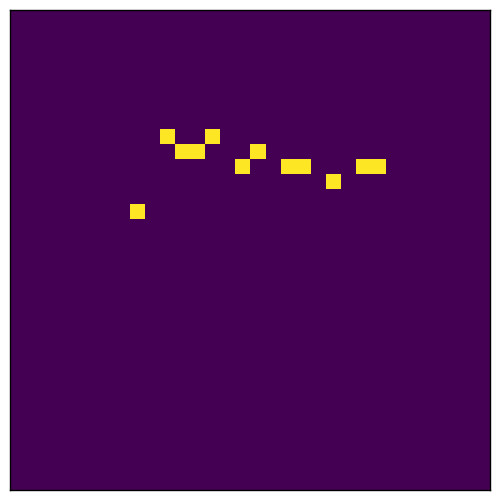
\includegraphics[height=2cm]{data/2d/input_df/0_input}
  \end{subfigure}
  \begin{subfigure}[t]{0.12\textwidth}
    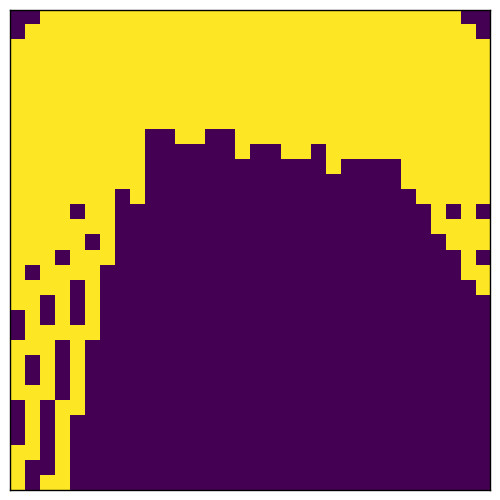
\includegraphics[height=2cm]{data/2d/input_df/0_space}
  \end{subfigure}
  \begin{subfigure}[t]{0.12\textwidth}
    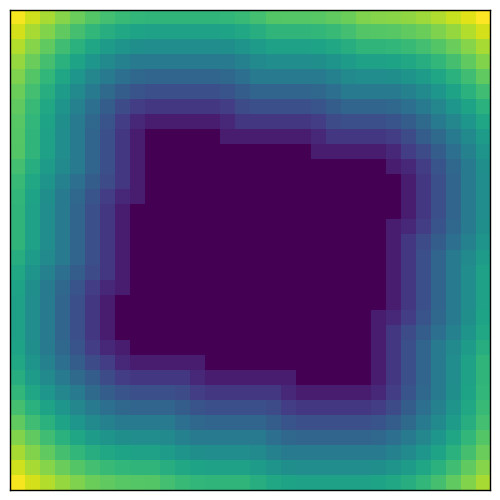
\includegraphics[height=2cm]{data/2d/input_df/0_output_df}
  \end{subfigure}
  \begin{subfigure}[t]{0.12\textwidth}
    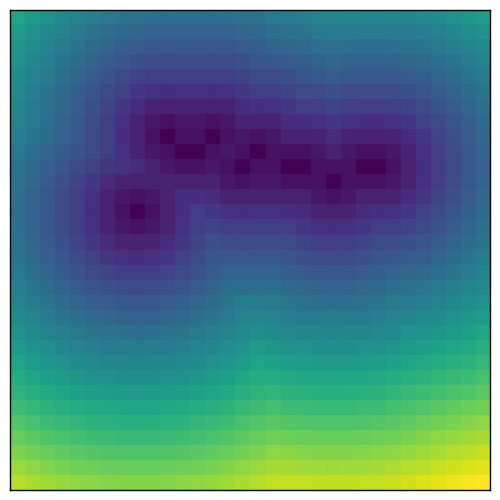
\includegraphics[height=2cm]{data/2d/input_df/0_input_df}
  \end{subfigure}
  \begin{subfigure}[t]{0.12\textwidth}
    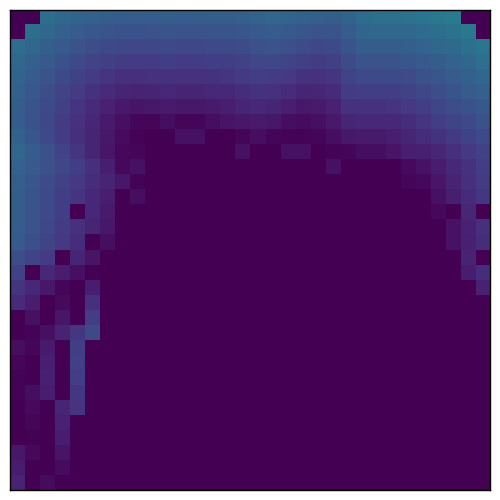
\includegraphics[height=2cm]{data/2d/input_df/0_err_space}
  \end{subfigure}\\

  \begin{subfigure}[t]{0.12\textwidth}
    
\includegraphics[height=2cm]{data/2d/input_df/2_output}
  \end{subfigure}
  \begin{subfigure}[t]{0.12\textwidth}
    
\includegraphics[height=2cm]{data/2d/input_df/2_input}
  \end{subfigure}
  \begin{subfigure}[t]{0.12\textwidth}
    
\includegraphics[height=2cm]{data/2d/input_df/2_space}
  \end{subfigure}
  \begin{subfigure}[t]{0.12\textwidth}
    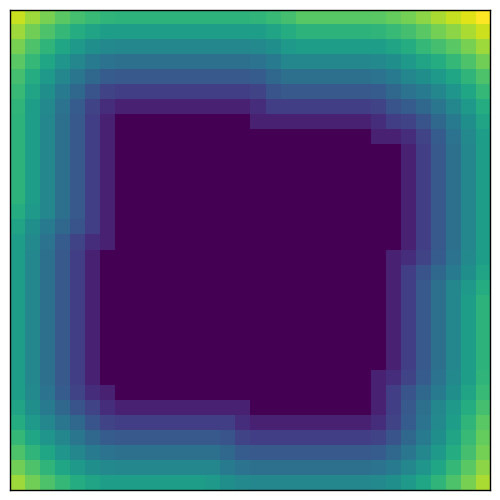
\includegraphics[height=2cm]{data/2d/input_df/2_output_df}
  \end{subfigure}
  \begin{subfigure}[t]{0.12\textwidth}
    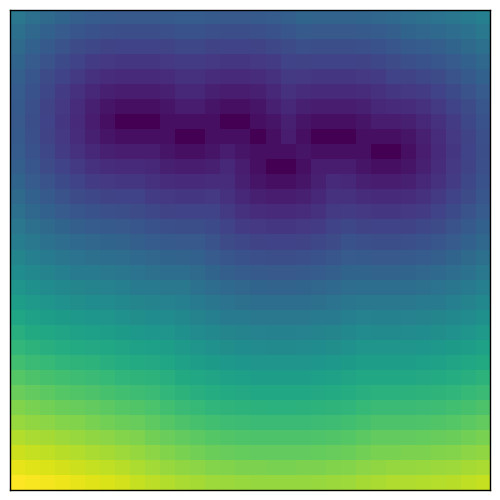
\includegraphics[height=2cm]{data/2d/input_df/2_input_df}
  \end{subfigure}
  \begin{subfigure}[t]{0.12\textwidth}
    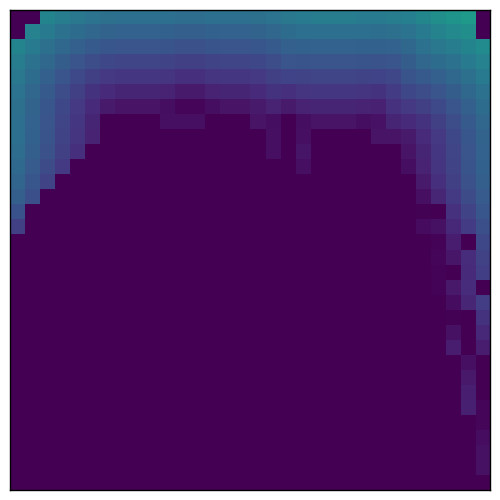
\includegraphics[height=2cm]{data/2d/input_df/2_err_space}
  \end{subfigure}

  % TODO short caption
  \caption{For implementing the negative log-likelihood $-\ln p(y_i = x_i | z)$
  using Gaussian, \ie continuous, predictions $y_i$, we ca derive (signed) distance
  functions from the given, binary observations $x_i$ for $x_i \neq \uk$ using
  a distance transform.
  %Note that when using real signed distance functions,
  %\ie representing the distance to the original mesh, we would compute
  %the distance to the observed points instead.
  A reasonable loss would then
  compute the negative log-likelihood for all voxels in free space.
  However, in the case of noisy observations,
  even the ground truth shape will have a high negative log-likelihood because
  distance values are affected significantly by few noisy observations.
  To illustrates this phenomenon we show the ground truth shape, the noisy
  observations and the free space in the first three columns for two examples
  from our synthetic 2D dataset, see Appendix \ref{ch:appendix-data}. The
  remaining columns show the distance function of the ground truth shape and
  the noisy observations as well as the the free-space-masked absolute error from
  Equation \eqref{eq:shape-inference-smerr}.}
  \label{fig:shape-inference-sdf-problem}
\end{figure}

When predicting signed distance functions, these are modeled using voxel-wise
Gaussians with fixed variance, \ie
\begin{align}
  p(y_i | z) = \mathcal{N}(y_i;\mu_i(z),\sigma^2).
\end{align}
Ideally, we would derive a signed distance function on our observations
in order to directly use the negative log likelihood $-\ln p(y_i = x_i | z)$ as loss. However,
this leads to a problem illustrated in Figure \ref{fig:shape-inference-sdf-problem}
where the ground truth shape has very high error when defining an absolute error between
the distance function $\text{df}(x_p)$ of observed points $x_p$ and the distance function
$\text{df}(y^*)$ of the ground truth shape $y^*$ when considering voxels in free space only, \ie
\begin{align}
  \sum_{i = 1}^R x_{f,i} \left|\text{df}_i(x_p) - \text{df}_i(y^*)\right|.
  \label{eq:shape-inference-smerr}
\end{align}
Here $x_p$ defines the occupancy grid corresponding to observed points only,
\ie $x_{p,i} = 1$ for $x_i = 1$ and $x_{p,i} = 0$ otherwise.
We also note that $\text{df}(x_p)$ computes, for each voxel, the distance
to the nearest occupied pixel $x_{p,i} = 1$. Similarly, $x_f$
is defined as the occupancy grid corresponding to free space voxels,
\ie $x_{f,i} = 1$ for $x_i = 0$ and $x_{f,i} = 0$ otherwise.
% TODO cite Andreas' paper
Of course, this method of deriving distance functions from the observations
is not ideal; for example, other authors \cite{SteinbrueckerCremers:2013}
compute a distance function along the rays from the observed points. However,
noisy observations are still problematic.%We leave this for future work.

As of the above discussion we would like to use binary observations while still predicting a
shape in signed distance function representation. Then, however, 
evaluating $p(y_i = x_i | z)$ is not meaningful. Instead we need to introduce
a transformation $\theta_i(\mu_i)$ quantifying the probability of occupancy
after having predicted a mean signed distance function value of $\mu_i$.
To this end, we take a closer look on the univariate Gaussian:

% TODO figure of Gaussian and CDF
\begin{figure}
  \centering
  \hspace*{-0.25cm}
  \begin{subfigure}[t]{0.48\textwidth}
    \centering
    \begin{tikzpicture}
      \begin{axis}[
          every axis plot post/.append style={
          mark=none,domain=-3:2,samples=50,smooth},
          axis x line*=bottom,
          axis y line*=left,
          enlargelimits=upper,
          ymax=1.1, ymin=0,
          ylabel=$p(y)$,
          xlabel=$y$,
          legend style={at={(0.65,1)},anchor=north west},
          height=5cm,
          width=7cm,
        ]
      
        \addplot[name path=g,blue] {gauss(-0.75,0.5)};
        \addlegendentry{$p(y)$};
        %\addplot[red] {gauss(1,0.5)};
        %\addlegendentry{$\mu_j(z) = -0.5; \sigma^2 = 0.5$};
        \addplot[blue,dashed,mark=none,forget plot] coordinates {(-0.75, 0) (-0.75, 1)};
        \node at (axis cs:-0.75,1.1) {$\mu_i(z)$};
      
        \addplot[black,dashed,mark=none,forget plot] coordinates {(0, 0) (0, 1)};
        \node at (axis cs:0,1.1) {$0$};
      
        %\addplot[red,dashed,mark=none] coordinates {(1, 0) (1, 0.9)};
        %\node at (axis cs:1,1) {$\mu_j(z)$};
      
        \path[name path=axis] (axis cs:-3,0) -- (axis cs:0,0);
        \addplot [
          thick,
          color=blue,
          fill=blue, 
          fill opacity=0.1,
          area legend, % https://tex.stackexchange.com/questions/246557/custom-area-legend-image-not-working
        ]
        fill between[
          of=g and axis,
          soft clip={domain=-3:0},
        ];
        \addlegendentry{$p(y \leq 0)$}
      \end{axis}
    \end{tikzpicture}
  \end{subfigure}\hfill
  \begin{subfigure}[t]{0.48\textwidth}
    \begin{tikzpicture}
      \begin{axis}[
          every axis plot post/.append style={
          mark=none,domain=-3:2,samples=50,smooth},
          axis x line*=bottom,
          axis y line*=left,
          enlargelimits=upper,
          ymax=1.1, ymin=0,
          ylabel=$p(y' \leq y)$,
          xlabel=$y$,
          legend style={at={(0.65,1)},anchor=north west},
          height=5cm,
          width=7cm,
        ]
      
        % 1.128379167 = 1/(0.5*sqrt(pi))
        \addplot[name path=g,blue] (\x,{0.5*(1 + erf((\x + 0.5)*1.128379167))});
        \addlegendentry{$p(y' \leq y)$};
        \addplot[black,dashed,mark=none,forget plot] coordinates {(0, -1) (0, 1)};
        \node at (axis cs:0,1.1) {$0$};
      \end{axis}
    \end{tikzpicture}
  \end{subfigure}
  %\vskip 6px
  % TODO short caption
  \caption{Illustration of a Gaussian distribution $p(y) = \mathcal{N}(y;-0.75,0.5^2)$
  on the left where the marked area corresponds to the probability $p(y \leq 0)$.
  In our case this refers to the probability of a voxel being occupied. The
  corresponding cumulative density function $p(y' \leq y)$ according to Equation
  \eqref{eq:shape-inference-cdf} is shown on the right.
  }
  \label{fig:shape-inference-gaussian}
\end{figure}

\begin{example}
  As defined in Definition \ref{def:deep-learning-gaussian}, the univariate
  Gaussian distribution takes the form in Figure
  \ref{fig:shape-inference-gaussian}. Its cumulative density
  function is given as
  \begin{align}
    \mathcal{N}(y' \leq y; \mu, \sigma^2) &= \int_{-\infty}^y \mathcal{N}(y'; \mu, \sigma^2) dy'\\
    &= \frac{1}{2}\left(1 + \erf\left(\frac{y - \mu}{\sigma \sqrt{2}}\right)\right).
    \label{eq:shape-inference-cdf}
  \end{align}
  and also shown in Figure \ref{fig:shape-inference-gaussian}.
  The error function $\erf$ is defined as
  \begin{align}
    \erf(y) = \frac{1}{\sqrt{\pi}} \int_{-y}^y \exp(-y'^2) dy'.
  \end{align}
  The cumulative density function quantifies the probability of a variable
  $y'$ falling into a specific range -- in our case $y'$ falling into $(-\infty,y]$.
\end{example}

Using the Gaussian cumulative density function we want to determine the
probability $\theta_i(\mu_i)$ of occupancy.
This process is illustrated in Figure \ref{fig:shape-inference-gaussian};
as negative values in a signed distance function refer to occupied voxels,
we can use
\begin{align}
  \theta_i(\mu_i) &= \mathcal{N}(y' \leq 0; \mu_i, \sigma^2)\\
  &=\frac{1}{2}\left(1 + \erf\left(\frac{- \mu_i}{\sigma \sqrt{\pi}}\right)\right).
  \label{eq:shape-inference-theta-mu-transformation}
\end{align}
Intuitively, we evaluate the cumulative density function at $0$ giving the probability
$\mathcal{N}(y \leq 0; \mu_i(z), \sigma^2)$ which corresponds to the probability of
occupancy. The negative log-likelihood can then be stated as
% TODO theta_i the i is unnecessary
\begin{align}
  \mathcal{L}_{\text{AML},\mathcal{N}}(w) = - \sum_{i = 1,x_i \neq \uk}^R \ln \Ber(y_i = x_i; \theta_i(\mu_i(z))) - \ln \mathcal{N}(z;0,I_Q).
\end{align}
The second term, the negative log-likelihood of the prior $p(z)$ is of course only
added once if the two losses $\mathcal{L}_{\text{AML},\mathcal{N}}$ and
$\mathcal{L}_{\text{AML},\Ber}$ are combined. As before, the negative log-likelihood
of the Bernoulli distributions $\Ber(y_i = x_i; \theta_i(\mu_i(z)))$ leads to the
binary cross entropy error.

\subsection{Practical Considerations}

In practice, we can predict a shape $y$ in both occupancy or signed
distance function representation or use either of them. Compared to
Figure \ref{fig:shape-inference-gaussian}, we generally use a small
variance such as $\ln \sigma^2 = -2 \Leftrightarrow \sigma^2 \approx 0.13533$.
In practice, the fixed variance merely scales the used sum-of-squared loss.
As a result, we found the fixed variance to have negligible impact on training
as long as it is not chosen too small, \eg $\sigma^2 > 0.01$, or too large,
\eg $\sigma^2 < 1$.
Then, for predicting a signed distance function, we add a post-processing layer
which explicitly implements the transformation $\theta(\mu(z))$ from
Equation \eqref{eq:shape-inference-theta-mu-transformation} and allows to
conveniently apply a binary cross entropy loss on top:

\begin{definition}
  A Gaussian to Bernoulli layer $\text{g2b}_{\sigma^2}$ takes as input
  a tensor $\mu \in \mathbb{R}^{B \times C \times H \times W \times D}$ corresponding
  to an element-wise predicted mean (\ie $\mu_i(z)$) of a signed
  distance function and computes a tensor of occupancy probabilities as
  \begin{align}
    (\text{g2b}_{\sigma^2}(\mu))_i &= \int_{-\infty}^0 \mathcal{N}(y_i; \mu_i, \sigma^2) dy_i\\
    &= \frac{1}{2}\left(1 + \erf\left(\frac{-\mu_i}{\sigma \sqrt{\pi}}\right)\right).
  \end{align}
\end{definition}

At this point we note that the derivative of the Gaussian to Bernoulli
layer, which essentially corresponds to the derivative of the Gaussian
cumulative density function, is a Gaussian distribution:
\begin{align}
  \frac{\partial \frac{1}{2}\left(1 + \erf\left(\frac{-\mu_i}{\sigma \sqrt{\pi}}\right)\right)}{\partial \mu_i} &= \left.\frac{\partial \erf(t)}{\partial t}\right|_{t = \frac{-\mu_i}{\sigma\sqrt{\pi}}} \frac{\partial \frac{-\mu_i}{\sigma\sqrt{\pi}}}{\partial \mu_i}\\
  &=\frac{1}{\sqrt{2\pi}\sigma} \exp\left( -\frac{1}{2} \frac{(-\mu_i)^2}{\sigma^2}\right)\\
  &= \mathcal{N}(0; \mu_i, \sigma^2).
\end{align}
The error function $\erf$ is in practice approximated following \cite{Abramowitz:1974}\footnote{
  We use code provided at \url{http://hewgill.com/picomath/lua/erf.lua.html}.
}. If we would additionally predict the variances $\sigma_i^2$, the
derivatives would be more involved, but we did not see any practical benefit of
doing so.
% TODO illustration of training process ... also for non-probabilistic approach!

For both predicting occupancy and signed distance functions,
we found that it is beneficial to weight the prior, \eg
\begin{align}
  \mathcal{L}_{\text{AML}}(w) = - \sum_{i = 1,x_i \neq \uk}^R \ln \Ber(y_i = x_i; \theta_i(z)) - \kappa \ln \mathcal{N}(z;0,I_Q);
  \label{eq:shape-inference-aml-weighted-loss}
\end{align}
especially on datasets with noise, it is important that the encoder
$z(x;w)$ learns to predict latent codes $z$ that are likely under the
unit Gaussian prior $p(z)$. This prevents the encoder from getting distracted
by noise which usually also leads to unlikely codes $z$.

\section{Extended Variational Auto-Encoder}

% TODO plate notation M,N or R/Q?
\begin{figure}
  \centering
  \hspace*{-0.5cm}
  \begin{subfigure}[t]{0.48\textwidth}
    \centering
    \begin{tikzpicture}

      \node[rectangle,rounded corners=0.05cm,draw=black,minimum width=2cm,minimum height=3.5cm] (M) at (0.25, -1){};
      \node[above left] at (M.south east){$M$};
      \node[circle,draw=black,minimum size=1cm] (z) at (0,0){$z$};
      \node[circle,draw=black,minimum size=1cm] (y) at (0,-2){$y$};
      \node[] (w) at (-2,0){$w$};
      
      \draw[->] (w) -- (z);
      \draw[->] (y) -- (z);
      
      \draw[-,dashed] (1.75,-3.1) -- (1.75,1.1);
      
      \node[rectangle,rounded corners=0.05cm,draw=black,minimum width=2cm,minimum height=3.5cm] (M) at (3.25, -1){};
      \node[above left] at (M.south east){$M$};
      \node[circle,draw=black,minimum size=1cm] (z) at (3,0){$z$};
      \node[circle,draw=black,minimum size=1cm] (y) at (3,-2){$y$};
      \node[] (w) at (5,0){$w$};
      
      \draw[->] (w) -- (z);
      \draw[->] (w) -- (y);
      \draw[->] (z) -- (y);
      
    \end{tikzpicture}
    \vskip 6px
    \caption{Illustration of the graphical model of the original variational
    auto-encoder as discussed in Chapter \ref{ch:shape-prior}.
    The generative model is shown on the right and governed by $p(y, z) = p(y|z)p(z)$,
    while the recognition model is shown on the left and
    approximated by $q(z|y)$.}
    \label{subfig:shape-inference-vae}
  \end{subfigure}\hfill
  \begin{subfigure}[t]{0.48\textwidth}
    \centering
    \begin{tikzpicture}

      \node[rectangle,rounded corners=0.05cm,draw=black,minimum width=2cm,minimum height=5.5cm] (M) at (0.25, -2){};
      \node[above left] at (M.south east){$N$};
      \node[circle,draw=black,minimum size=1cm] (z) at (0,0){$z$};
      \node[circle,draw=black,minimum size=1cm] (y) at (0,-2){$y$};
      \node[circle,draw=black,minimum size=1cm] (x) at (0,-4){$x$};
      \node[] (w) at (-2,0){$w$};
      
      \draw[->] (w) -- (z);
      %\draw[->] (y) -- (z);
      \draw[->,dashed] (x) -- (y);
      \draw[->] (x) to [out=45,in=315](z);
      
      \draw[-,dashed] (1.75,-5.1) -- (1.75,1.1);
      
      \node[rectangle,rounded corners=0.05cm,draw=black,minimum width=2cm,minimum height=5.5cm] (M) at (3.25, -2){};
      \node[above left] at (M.south east){$N$};
      \node[circle,draw=black,minimum size=1cm] (z) at (3,0){$z$};
      \node[circle,draw=black,minimum size=1cm] (y) at (3,-2){$y$};
      \node[circle,draw=black,minimum size=1cm] (x) at (3,-4){$x$};
      \node[] (w) at (5,0){$w$};
      
      \draw[->] (w) -- (z);
      \draw[->] (w) -- (y);
      \draw[->] (w) -- (x);
      \draw[->] (z) -- (y);
      \draw[->] (y) -- (x);

    \end{tikzpicture}
    \vskip 6px
    % TODO text model
    \caption{Illustration of the graphical model of the extended
  variational auto-encoder explicitly taking into account the observation $x$.
  The generative model on the right assumes that first a shape $y$
  is generated through $p(y | z)$ and the observation $x$ is then
  obtained from the observation model $p(x | y)$. In the inference model on
  the left the latent code $z$ is inferred through $q(z | x)$ -- this can be
  seen as probabilistic embedding of observation $x$ in the latent shape space.
  The (dashed) model $q(y | x)$ is not learned but used to tie the observation $x$
  to the predicted shape $y$.}
    \label{subfig:shape-inference-evae}
  \end{subfigure}
  \vskip 6px
  % TODO short caption
  \caption{Comparison of the regular variational auto-encoder model in Figure
  \ref{subfig:shape-inference-vae} to learn a shape prior and the 
  extended variational auto-encoder model to learn shape completion in
  Figure \ref{subfig:shape-inference-evae}.}
  \label{fig:shape-inference}
\end{figure}

The approaches discussed above are formulated in a maximum likelihood framework
where we consider $x_i$ to be actual observations of the random variables $y_i$. In contrast,
we might also directly extend the graphical model in Figure \ref{subfig:shape-inference-vae}
to also consider the observation $x_i$ as random variable.
In Figure \ref{subfig:shape-inference-evae}
we illustrate a possible extension that we decided to investigate closer.
The main idea is to model the observation process $p(x | y)$ explicitly in order
to deduce information about a possible $y$. There are many possibilities to
model $p(x | y)$ -- \eg by learning it directly from samples $\{(x_n, y_n^*)\}$
or by modeling the sensor. Here, we leave these options for future work
and model $p(x | y)$ through a neural network without direct supervision
by embedding $p(x | y)$ in the framework of variational inference.

Following the introduction of variational inference in Section \ref{sec:variational-inference},
the evidence lower bound for the model in Figure \ref{subfig:shape-inference-evae} can be
written as
\begin{align}
  - \text{KL}(q(y,z|x)|p(y,z)) + \mathbb{E}_{q(y,z|x)}[\ln p(x|y)]
\end{align}
This formulation treats both $y$ and $z$ as latent variables regarding the
newly introduced random variable $x$. The exact structure of $q(y,z|x)$ as well
as $p(y,z)$ is not defined yet. For the latter we again use a pre-trained shape prior
$p(y,z) = p(y|z) p(z)$; for the former we have to make simplifying assumptions.
In particular, we assume that $y$ and $z$ are statistically independent given $x$:
\begin{align}
  q(y, z | x) = q(y | x) q(z | x).
\end{align}
Here, $q(z | x)$ is the mapping we want to learn; $p(y | x)$ decomposes into
\begin{align}
  q(y | x) = \prod_{i = 1}^R q(y_i | x_i)
\end{align}
and can easily be modeled for those voxels $x_i$ where we have observations, \ie
$x_i \neq \uk$. Note that $q(y | x)$ is not learned, \ie it is
not modeled through a neural network -- it is not part of the recognition model;
however $q(y | x)$ allows us to integrate
knowledge about the observations within the Kullback-Leibler divergence:
\begin{align}
  \text{KL}(q(y,z|x)|p(y,z)) &= \mathbb{E}_{q(y, z | x)}\left[\ln\frac{q(y, z | x)}{p(y, z)}\right]\\
  &= \mathbb{E}_{q(y, z | x)}\left[\ln\frac{q(y | x)q(z | x)}{p(y | z)p(y)}\right]\\
  &= \mathbb{E}_{q(y | x)}\left[\ln\frac{q(y | x)}{p(y | z)}\right] + \mathbb{E}_{q(z | x)}\left[\ln\frac{q(z | x)}{p(z)}\right]\\
  &= \KL(q(y|x) | p(y|z)) + \KL(q(z|x)|p(z))
\end{align}
Finally, the reconstruction error simplifies to
\begin{align}
  \mathbb{E}_{q(y,z|x)}[\ln p(x|y)] = \mathbb{E}_{q(y|x)}[\ln p(x|y)].
\end{align}
Then, the overall objective can then be written as
\begin{align}
  \mathcal{L}_{\text{EVAE}}(w) = \text{KL}(q(z | x)|p(z)) + \text{KL}(q(y | x)|p(y | z)) 
  - \mathbb{E}_{q(y | x)}[\ln p(x | y)]
  \label{eq:shape-inference-evae}
\end{align}
where the Kullback-Leibler divergence $\text{KL}(q(y | x)|p(y | z))$ implicitly
ties the observation $x$ to the possible shape $y$.

% TODO introduce concept of Monte Carlo samples
As before, both Kullback-Leibler divergences can be computed analytically. Only
the reconstruction error $\mathbb{E}_{q(y|x)}[\ln p(x|y)]$ needs to be 
approximated using Monte-Carlo samples; for a specific sample $x_n$, this means
\begin{align}
  - \mathbb{E}_{q(y | x)}[\ln p(x | y)] = - \sum_{l = 1}^L \ln p(x_n | y_{l,n})
\end{align}
% TODO multiariate uniform distribution ...
with
\begin{align}
  y_{l,n} &= g_y(z_{l,n}, \epsilon_{l,n})\quad\text{ and }\quad\epsilon_{l,n} \sim U(0,1)^R\\
  z_{l,n} &= g_z(x_n, \epsilon'_{l,n})\quad\text{ and }\quad\epsilon'_{l,n} \sim \mathcal{N}(\epsilon;0,I_Q)
\end{align}
and usually using $L = 1$ sample. Here, $g_y$ represents the Bernoulli
reparameterization trick from
Section \ref{sec:shape-prior-bernoulli-vae} and $g_z$ the Gaussian equivalent
from Section \ref{sec:shape-prior-gaussian-vae}. This also implies that
$y_i$ is modeled using a Bernoulli distribution, just like $x_i$, while
$z$ is modeled using a Gaussian distribution. To make this explicit,
we write
% TODO theta and rho?
\begin{align}
  p(z) &= \mathcal{N}(z;\mu(x), \diag(\sigma^2(x)))\\
  p(y_i | z) &= \Ber(y_i;\theta_i(z))\\
  p(x_i | y) &= \Ber(x_i;\rho_i(y))
\end{align}
where the parameters $\mu$, $\sigma^2$ as well as $\theta_i$, $\rho_i$
are modeled using neural networks; in particular, $\theta_i(z)$ is taken
from the pre-trained shape prior in order to restrict shape inference to
reasonable shapes. Overall,
this specifies the generative model of the extended variational auto-encoder
as in Figure \ref{subfig:shape-inference-evae} on the right.

In Equation \eqref{eq:shape-inference-evae}, only the Kullback-Leibler divergence
$\KL(q(y|x)|p(y|z))$ as well as the recognition model $q(z|x)$ are left
for discussion. The approximate posterior $q(z|x)$ is modeled analogously
to $q(z|y)$. For the Kullback-Leibler divergence, we follow the
maximum likelihood formulation and use:
\begin{align}
  q(y_i | x_i = 1) &= \Ber(y_i; 1)\\
  q(y_i | x_i = 0) &= \Ber(y_i; 0)
\end{align}
while ignoring unobserved voxels $x_i = \uk$ as we assume a strong enough 
shape prior that is able to fill in the unobserved voxels.
The Kullback-Leibler divergence $\KL(q(y|x)|p(y|z))$ then implicitly tries to
adjust the predicted shape $y$ to the observation $x$.

\subsection{Practical Considerations}

% TODO implementation details with figure
We already introduced all the necessary
tools for implementing the proposed model in Chapter \ref{ch:shape-prior}.
The latent code $z$ is still modeled as Gaussian;
so, for the Kullback-Leibler divergence $\KL(q(z|x) | p(z))$ Equation
\eqref{eq:shape-prior-analyitcal-kld} applies:
\begin{align}
  \KL(q(z|x) | p(z)) &= \sum_{i = 1}^Q \KL(\mathcal{N}(z_i; \mu_i(x), \sigma_i(x)^2) | \mathcal{N}(z_i; 0, 1))\\
  &= \sum_{i = 1}^Q \left(- \frac{1}{2} \ln \sigma_i(x) + \frac{1}{2} \sigma_i(x)^2 + \frac{1}{2} \mu_i^2(x) - \frac{1}{2}\right).
\end{align}
The voxels $y_i$ are modeled using Bernoulli distributions and $p(y|z)$
is taken from the shape prior; it is not fine-tuned but
kept fixed. The Kullback-Leibler divergence $\KL(q(y|x)|p(y|z))$ 
follows Equation \eqref{eq:shape-prior-bernoulli-kld} and can be written as
\begin{align}
  \KL(q(y&|x)|p(y|z)) = \sum_{i = 1}^R \KL(q(y_i|x_i)|p(y_i|z))\\
  &= \sum_{i = 1, x_i \neq \uk}^R \sum_{k \in \{0,1\}} \left.\begin{cases}
    \ln 1^k 0^{1 - k} & \quad x_i = 1\\
    \ln 0^k 1^{1 - k} & \quad x_i = 0
  \end{cases}\right\} - \ln \theta_i(z)^k (1 - \theta_i(z))^{1-k}.
  \label{eq:shape-inference-evae-kld}
\end{align}
In practice, for numerical reasons, we need to add a small $\epsilon$-term
to avoid taking the natural logarithm $\ln 0$, \ie $\ln \theta^k (1-\theta)^k$
becomes $\ln (\theta + \epsilon)^k (1 - \theta + \epsilon)^{1 - k}$.
The pre-trained generative model $p(y | z)$ is then followed by a Bernoulli
Kullback-Leibler layer (\cf Definition \ref{def:shape-prior-bernoulli-kld})
implementing Equation \eqref{eq:shape-inference-evae-kld}
and a Bernoulli reparameterization layer (\cf Definition \ref{def:shape-prior-bernoulli-repa}).
The observation model $p(x | y)$ is then learned using a 3D convolutional neural
network as illustrated in Figure \ref{fig:shape-inference-evae}.
% TODO example

% TODO light gray, surround the individual parts, i.e.
% q(z|x), p(y|z) and p(x|y)
%\begin{figure}
%  \centering
%  \begin{tikzpicture}
%    \node (x) at (0,0) {$x$};
%
%    \node[conv,rotate=90,minimum width=4cm] (conv1) at (1.25,0) {$\text{conv}_{1, C_1, K}$ + $\text{bn}$ + $h$};
%    \node[pool,rotate=90,minimum width=4cm] (pool1) at (2.5,0) {$\text{pool}_{2}$};
%    \node[conv,rotate=90,minimum width=4cm] (conv2) at (3.75,0) {$\text{conv}_{C_1, C_2, K}$ + $\text{bn}$ + $h$};
%    \node[pool,rotate=90,minimum width=4cm] (pool2) at (5,0) {$\text{pool}_{2}$};
%    \node[view,rotate=90,minimum width=4cm] (view2) at (6.25,0) {$\text{view}_{B, C_3}$};
%    
%    \node[fc,rotate=90, minimum width = 1.8625cm] (fc21) at (8,1.07525) {$\text{fc}_{C_3, Q}$};
%    \node[fc,rotate=90, minimum width = 1.8625cm] (fc22) at (8,-1.07525) {$\text{fc}_{C_3, Q}$};
%  
%    \node at (9, 1.15){$\mu$};
%    \node at (9, -1.15){$\sigma^2$};
%  
%    \node[view,rotate=90,minimum width=4cm] (kld1) at (10,0) {$\text{KLD}_{\mathcal{N}}$};
%    \node[view,rotate=90,minimum width=4cm] (repa1) at (12,0) {$\text{repa}_{\mathcal{N}}$};
%    
%    \node at (11,0.3){$\mu,\sigma^2$};
%    
%    \node (z) at (13.5,-2.5){$z$};
%    
%    \node[fc,rotate=90,minimum width=4cm] (fc3) at (12,-5) {$\text{fc}_{Q, C_3}$};
%    \node[view,rotate=90,minimum width=4cm] (view3) at (10.75,-5) {$\text{view}_{B, C_2, \floor{\frac{H}{4}}, \floor{\frac{W}{4}}, \floor{\frac{D}{4}}}$};
%    
%    \node[up,rotate=90,minimum width=4cm] (up4) at (9.5,-5) {$\text{nnup}_{2}$};
%    \node[conv,rotate=90,minimum width=4cm] (conv4) at (8.25,-5) {$\text{conv}_{C_2, C_1, K}$ + $\text{bn}$ + $h$};
%    
%    \node[up,rotate=90,minimum width=4cm] (up5) at (7,-5) {$\text{nnup}_{2}$};
%    \node[conv,rotate=90,minimum width=4cm] (conv5) at (5.75,-5) {$\text{conv}_{C_1, 1, K}$ + $\text{bn}$ + $h$};
%    
%    \node at (4.75,-4.7){$\theta$};
%    
%    \node[view,rotate=90,minimum width=4cm] (kld2) at (3.75,-5) {$\text{KLD}_{\Ber}$};
%    
%    \node at (2.75,-4.7){$\theta$};
%    
%    \node[view,rotate=90,minimum width=4cm] (repa2) at (1.75,-5) {$\text{repa}_{\Ber}$};
%    
%    \node (y) at (0,-7.5) {$\tilde{y}$};
%    
%    \node[conv,rotate=90,minimum width=4cm] (conv6) at (1.25,-10) {$\text{conv}_{1, C_4, K}$ + $\text{bn}$ + $h$};
%    \node[conv,rotate=90,minimum width=4cm] (conv7) at (2.5,-10) {$\text{conv}_{C_4, C_5, K}$ + $\text{bn}$ + $h$};
%    \node[conv,rotate=90,minimum width=4cm] (conv8) at (3.75,-10) {$\text{conv}_{C_5, C_1, K}$ + $\text{bn}$ + $h$};
%    
%    \node (rx) at (13.5, -10) {$\tilde{x}$};
%    
%    \draw[->] (x) -- (conv1);
%    \draw[->] (conv1) -- (pool1);
%    \draw[->] (pool1) -- (conv2);
%    \draw[->] (conv2) -- (pool2);
%    \draw[->] (pool2) -- (view2);
%    \draw[->] (view2) -- (fc21);
%    \draw[->] (view2) -- (fc22);
%    \draw[->] (fc21) -- (kld1);
%    \draw[->] (fc22) -- (kld1);
%    \draw[->] (kld) -- (repa1);
%    \draw[-] (repa1) -- (13.5,0);
%    \draw[->] (13.5,0) -- (z);
%    \draw[-] (z) -- (13.5,-5);
%    \draw[->] (13.5,-5) -- (fc3);
%    \draw[->] (fc3) -- (view3);
%    \draw[->] (view3) -- (up4);
%    \draw[->] (up4) -- (conv4);
%    \draw[->] (conv4) -- (up5);
%    \draw[->] (up5) -- (conv5);
%    \draw[->] (conv5) -- (kld2);
%    \draw[->] (kld2) -- (repa2);
%    \draw[-] (repa2) -- (0,-5);
%    \draw[->] (0,-5) -- (y);
%    \draw[-] (y) -- (0,-10);
%    \draw[->] (0,-10) -- (conv6);
%    \draw[->] (conv6) -- (conv7);
%    \draw[->] (conv7) -- (conv8);
%    \draw[->] (conv8) -- (rx);
%  \end{tikzpicture}
%  \vskip 6px
%  
%  \caption{Illustration of the extended variational auto-encoder. For
%  comparison, we also consider Figure \ref{fig:shape-prior-variational-auto-encoder}
%  of the standard variational auto-encoder. Here, both $q(z|x)$ and $p(y|z)$
%  are represented by convolutional neural networks mirroring each other;
%  each consisting of two stages of convolutional layers including batch normalization,
%  non-linearity and pooling.
%  The decoder, \ie $p(y|z)$, is kept fixed after pre-training; the encoder
%  $q(z|x)$ is either trained from scratch or fine-tuned from $q(z|y)$.
%  The last part, the convolutional neural network modeling $p(x|y)$, consists
%  of three stages of convolutional layers including batch normalization and non-linearity.
%  Here, no pooling layers can be found as the size of the output $x$
%  matches the size of its input $y$.}
%  \label{fig:shape-inference-evae}
%\end{figure}

\begin{figure}
  \centering
  \hspace*{-0.75cm}
  \begin{tikzpicture}
    \node (x) at (0,0) {\small$x$};

    \node[conv,rotate=90,minimum width=4.5cm] (conv1) at (2.5,0) {\small$\text{conv}_{1, 16, 3}$\,+\,$\text{bn}$\,+\,$\ReLU$};
    \node[pool,rotate=90,minimum width=4.5cm] (pool1) at (3.75,0) {\small$\text{pool}_{2}$};
    \node[conv,rotate=90,minimum width=4.5cm] (conv2) at (5,0) {\small$\text{conv}_{16, 32, 3}$\,+\,$\text{bn}$\,+\,$\ReLU$};
    \node[pool,rotate=90,minimum width=4.5cm] (pool2) at (6.25,0) {\small$\text{pool}_{2}$};
    \node[conv,rotate=90,minimum width=4.5cm] (conv3) at (7.5,0) {\small$\text{conv}_{32, 64, 3}$\,+\,$\text{bn}$\,+\,$\ReLU$};
    \node[pool,rotate=90,minimum width=4.5cm] (pool3) at (8.75,0) {\small$\text{pool}_{2}$};
    \node[conv,rotate=90,minimum width=4.5cm] (conv4) at (10,0) {\small$\text{conv}_{64, 128, 3}$\,+\,$\text{bn}$\,+\,$\ReLU$};
    \node[pool,rotate=90,minimum width=4.5cm] (pool4) at (11.25,0) {\small$\text{pool}_{2}$};
    
    \node[view,rotate=90,minimum width=4.5cm] (view4) at (12.5,0) {\small$\text{view}_{B, 1024}$};
    
    \node[fc,rotate=90, minimum width = 2cm] (fc51) at (13.75,1.25) {\small$\text{fc}_{512, Q}$};
    \node[fc,rotate=90, minimum width = 2cm] (fc52) at (13.75,-1.25) {\small$\text{fc}_{512, Q}$};
  
    \node[view,rotate=90,minimum width=4.5cm] (kld) at (15,0) {\small$\text{KLD}_{\mathcal{N}}$\,+\,$\text{repa}_{\mathcal{N}}$};
    
    \node (z) at (15,-5){\small$\tilde{z}$};
    
    \node[fc,rotate=90,minimum width=4.5cm] (fc6) at (13.75,-5) {\small$\text{fc}_{Q, 512}$};
    \node[view,rotate=90,minimum width=4.5cm] (view6) at (12.5,-5) {\small$\text{view}_{B, 1024, 2, 2, 2}$};
    
    \node[up,rotate=90,minimum width=4.5cm] (up7) at (11.25,-5) {\small$\text{nnup}_{2}$};
    \node[conv,rotate=90,minimum width=4.5cm] (conv7) at (10,-5) {\small$\text{conv}_{128, 64, 3}$\,+\,$\text{bn}$\,+\,$\ReLU$};
    \node[up,rotate=90,minimum width=4.5cm] (up8) at (8.75,-5) {\small$\text{nnup}_{2}$};
    \node[conv,rotate=90,minimum width=4.5cm] (conv8) at (7.5,-5) {\small$\text{conv}_{64, 32, 3}$\,+\,$\text{bn}$\,+\,$\ReLU$};
    \node[up,rotate=90,minimum width=4.5cm] (up9) at (6.25,-5) {\small$\text{nnup}_{2}$};
    \node[conv,rotate=90,minimum width=4.5cm] (conv9) at (5,-5) {\small$\text{conv}_{32, 16, 3}$\,+\,$\text{bn}$\,+\,$\ReLU$};
    \node[up,rotate=90,minimum width=4.5cm] (up10) at (3.75,-5) {\small$\text{nnup}_{2}$};
    \node[conv,rotate=90,minimum width=4.5cm] (conv10) at (2.5,-5) {\small$\text{conv}_{16, 1, 3}$\,+\,$\text{bn}$\,+\,$h$};
    
    \node[view,rotate=90,minimum width=4.5cm] (kld2) at (1.25,-5) {\small$\text{KLD}_{\Ber}$\,+\,$\text{repa}_{\Ber}$\,+\,$\sigma$};
    \node (ry) at (0,-5) {\small$\tilde{y}$};
    
    \node[conv,rotate=90,minimum width=4.5cm] (conv11) at (1.25,-10) {\small$\text{conv}_{1, 16, 3}$\,+\,$\text{bn}$\,+\,$\ReLU$};
    \node[conv,rotate=90,minimum width=4.5cm] (conv12) at (2.5,-10) {\small$\text{conv}_{16, 32, 3}$\,+\,$\text{bn}$ + $\ReLU$};
    \node[conv,rotate=90,minimum width=4.5cm] (conv13) at (3.75,-10) {\small$\text{conv}_{32, 64, 3}$\,+\,$\text{bn}$\,+\,$\ReLU$};
    \node[conv,rotate=90,minimum width=4.5cm] (conv14) at (5,-10) {\small$\text{conv}_{64, 128, 3}$\,+\,$\text{bn}$\,+\,$\ReLU$};
    \node[conv,rotate=90,minimum width=4.5cm] (conv15) at (6.25,-10) {\small$\text{conv}_{128, 64, 3}$\,+\,$\text{bn}$\,+\,$\ReLU$};
    \node[conv,rotate=90,minimum width=4.5cm] (conv16) at (7.5,-10) {\small$\text{conv}_{64, 32, 3}$\,+\,$\text{bn}$\,+\,$\ReLU$};
    \node[conv,rotate=90,minimum width=4.5cm] (conv17) at (8.74,-10) {\small$\text{conv}_{32, 16, 3}$\,+\,$\text{bn}$\,+\,$\ReLU$};
    \node[conv,rotate=90,minimum width=4.5cm] (conv18) at (10,-10) {\small$\text{conv}_{16, 1, 3}$\,+\,$\text{bn}$\,+\,$\sigma$};
    
    \node (rx) at (15, -10) {\small$\tilde{x}$};
    
    \draw[->] (y) -- (conv1);
    \draw[->] (conv1) -- (pool1);
    \draw[->] (pool1) -- (conv2);
    
    \draw[->] (conv2) -- (pool2);
    \draw[->] (pool2) -- (conv3);
    
    \draw[->] (conv3) -- (pool3);
    \draw[->] (pool3) -- (conv4);
    
    \draw[->] (conv4) -- (pool4);
    \draw[->] (pool4) -- (view4);
    
    \draw[->] (view4) -- (fc51);
    \draw[->] (view4) -- (fc52);
    
    \draw[->] (fc51) -- (kld);
    \draw[->] (fc52) -- (kld);
    
    \draw[->] (kld) -- (z);
    \draw[->] (z) -- (fc6);
    \draw[->] (fc6) -- (view6);
    
    \draw[->] (view6) -- (up7);
    \draw[->] (up7) -- (conv7);
    
    \draw[->] (conv7) -- (up8);
    \draw[->] (up8) -- (conv8);
    
    \draw[->] (conv8) -- (up9);
    \draw[->] (up9) -- (conv9);
    
    \draw[->] (conv9) -- (up10);
    \draw[->] (up10) -- (conv10);
    
    \draw[->] (conv10) -- (kld2);
    \draw[->] (kld2) -- (ry);
    \draw[-] (ry) -- (0, -10);
    \draw[->] (0, -10) -- (conv11);
    
    \draw[->] (conv11) -- (conv12);
    \draw[->] (conv12) -- (conv13);
    
    \draw[->] (conv13) -- (conv14);
    \draw[->] (conv14) -- (conv15);
    
    \draw[->] (conv15) -- (conv16);
    \draw[->] (conv16) -- (conv17);
    
    \draw[->] (conv17) -- (conv18);
    \draw[->] (conv18) -- (rx);

    \node[rotate=90] (L2) at (15, -11.5) {\small$\mathcal{L}(\tilde{x}, x)$};
    \draw[-,dashed] (rx) -- (L2);

    \node[rotate=90] (L1) at (0, 1.5) {\small$\mathcal{L}(\tilde{x}, x)$};
    \draw[-,dashed] (x) -- (L1);

    \node[rotate=90] (KLD2) at (0, -2.5) {\small$\KL(p(y|x)|p(y|z))$};
    \draw[-,dashed] (ry) -- (KLD2);

    \node[rotate=90] (KLD1) at (15, -7.5) {\small$\KL(q(z|y)|p(z))$};
    \draw[-,dashed] (z) -- (KLD1);
  \end{tikzpicture}
  \vskip 6px
  \caption{Illustration of the extended variational auto-encoder as
  also used in our experiments in Chapter \ref{ch:experiments}.
  It is worth comparing the illustrated implementation with Figure
  \ref{subfig:experiments-2d-architecture-vae} to understand that the
  generative model $p(y | z)$ are taken from the shape prior and the new
  recognition model $q(z | x)$ follows the architecture of $q(y| z)$. 
  In particular, the decoder, \ie $p(y|z)$, is kept fixed after learning the shape prior.
  The only completely new part is the convolutional neural network implementing the
  observation model $p(x|y)$. It consists of
  of eight convolutional stages including batch normalization and non-linearity.
  Here, no pooling layers can be found as the size of the output $x$
  matches the size of its input $y$. We additionally make the loss $\mathcal{L}(\tilde{x}, x)$
  between reconstructed observation $\tilde{x}$ and original observation $x$
  as well as the Kullback-Leibler divergences $\KL(q(z|y)|p(z))$, for the prior $p(z)$,
  and $\KL(p(y|x)|p(y|z))$, tying observations to predicted shapes, explicit.}
  \label{fig:shape-inference-evae}
\end{figure}

\section{Discussion}

Overall, we presented two approaches to tackle shape completion in a probabilistic
framework based on a pre-trained shape prior and without explicit superviseion.
Maximum likelihood, for example,
is a natural approach and can be related to works such as
\cite{EngelmannStuecklerLeibe:2016,EngelmannLeibe:2017} and \cite{DameReid:2013}
where shapes are modeled using PCA and GP-LVM,respectively,
and shape completion is formulated as energy minimization problem.
Using amortized maximum likelihood we intend to avoid the explicit optimization
problem required for inference and additionally consider both occupancy
and signed distance functions. We presented a formulation
that allows to use both representations with binary observations -- \eg in the form of
observed points and free space. Finally, the extended variational auto-encoder
presents an attempt to integrate the observations into the probabilistic framework
of variational inference. This model leaves several interesting questions for
future work, \eg how the observation model $p(x|y)$ can be modeled explicitly.
We will see in Chapter \ref{ch:experiments}, that both amortized maximum likelihood
as well as the extended variational auto-encoder perform well and inherently
optimize a similar objective.

  \chapter{Data}
\label{ch:data}

% TODO get rid of LiDAR!
For our formulation of shape completion,\ie Problem \ref{problem}, we require two sources
of data: the shape set $\mathcal{Y}$ to learn the shape prior and the observations $\mathcal{X}$
in order to learn maximum likelihood or an extended variational auto-encoder.
For research purposes,
however, we created three synthetic datasets also including the ground truth
shapes $\mathcal{Y}^*$ corresponding to $\mathcal{X}$ for evaluation: a
dataset of rectangles in 2D, a dataset of cuboids in 3D and
a dataset of cars from ShapeNet \cite{ChangFunkhouserGuibasSavarese:2015}
in 3D. Besides providing both observations $\mathcal{X}$ and ground
truth $\mathcal{Y}^*$, these datasets also
reflect the progress made in the course of the thesis. For brevity,
we will only present experiments in 3D; details on the
2D dataset can be found in Appendix~\ref{ch:appendix-data}.
Furthermore, we present experiments on the point clouds provided
by KITTI \cite{GeigerLenzUrtasun:2012,GeigerLenzStillerUrtasun:2013}.
In this case, we use car models from ShapeNet as shape set~$\mathcal{Y}$
and the provided 3D bounding boxes to extract the corresponding observations~$\mathcal{X}$.
However, on KITTI, we are not able to quantitatively
evaluate the proposed approaches due to missing ground truth shapes $\mathcal{Y}^*$.
In the following, we introduce our process of generating synthetic 3D datasets,
\ie the 3D cuboids dataset and the ShapeNet dataset, and extracting the observations
from KITTI.

\section{3D Example and ShapeNet}
\label{sec:data-3d}

Our 3D datasets consist of arbitrarily scaled and rotated
cuboids or cars; the cuboids are generated on-the-fly, while we use the
car models from ShapeNet.
The models are provided in the form of triangular meshes such that we
need to consider the following processing steps: voxelization and filling
of the shapes; rendering, backprojecting and voxelization of the observations;
and finally post-processing to compute signed distance functions. 
This will provide us with both observations and ground truth shapes; to
learn the shape prior, and simulate the realistic case,
we then voxelize and fill a separate set of shapes. The overall
process is also illustrated in Figure \ref{fig:data-3d-process} and discussed in
detail in the following.

\begin{figure}
  \centering
  \vspace{-1cm}
  \begin{tikzpicture}
    \node[
      %rectangle,draw=black
    ] at (-1, 0) {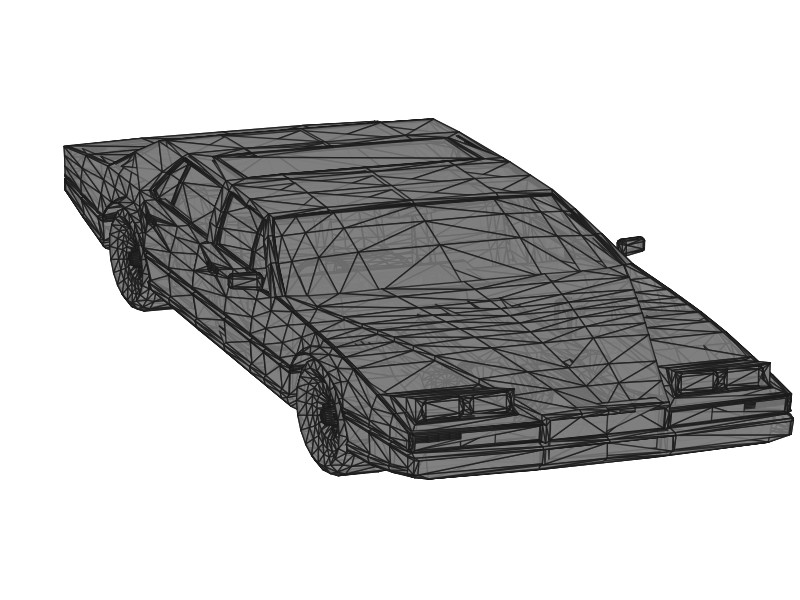
\includegraphics[height=2.25cm]{data/shapenet/dd84236f0ef27765a134736201a79843}};
    
    \node at (4, 0) {
\includegraphics[height=3cm]{data/shapenet/0}};
    %\node at (4, -2.5) {
\includegraphics[height=3cm]{data/shapenet/1}};
    %\node[rectangle,draw=black,minimum width=3.75cm,minimum height=5cm] at (4,-1.25) {};
    
    \node at(9, 0) {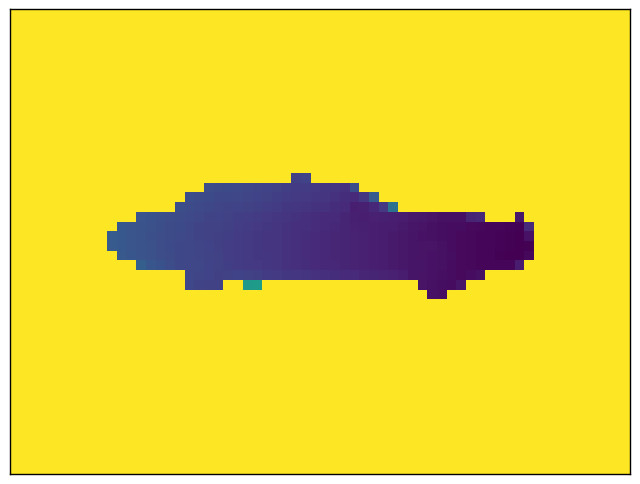
\includegraphics[height=2.5cm]{data/shapenet/0_depth}};
    %\node at(9, -2.5cm) {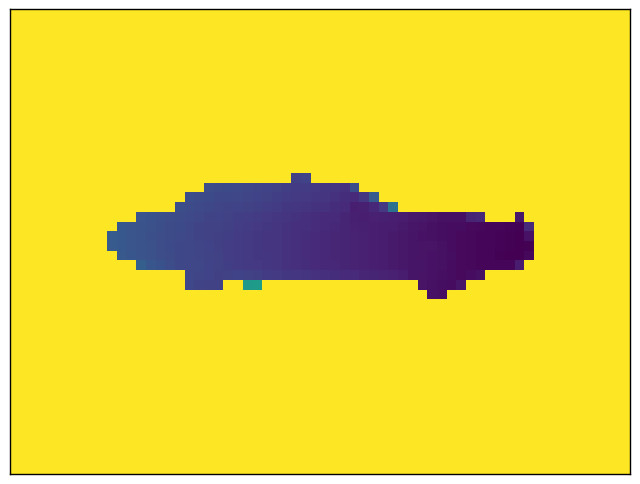
\includegraphics[height=2.5cm]{data/shapenet/0_depth}};
    %\node[rectangle,draw=black,minimum width=3.35cm,minimum height=5cm] at (9,-1.25) {};
    
    \draw[->] (1, 0) -- (2, 0);
    \node at (1.5,0.3) {(a)};
    
    \draw[->] (6, 0) -- (7, 0);
    \node at (6.5,0.3) {(b)};
    
    \node at (4, -3.5) {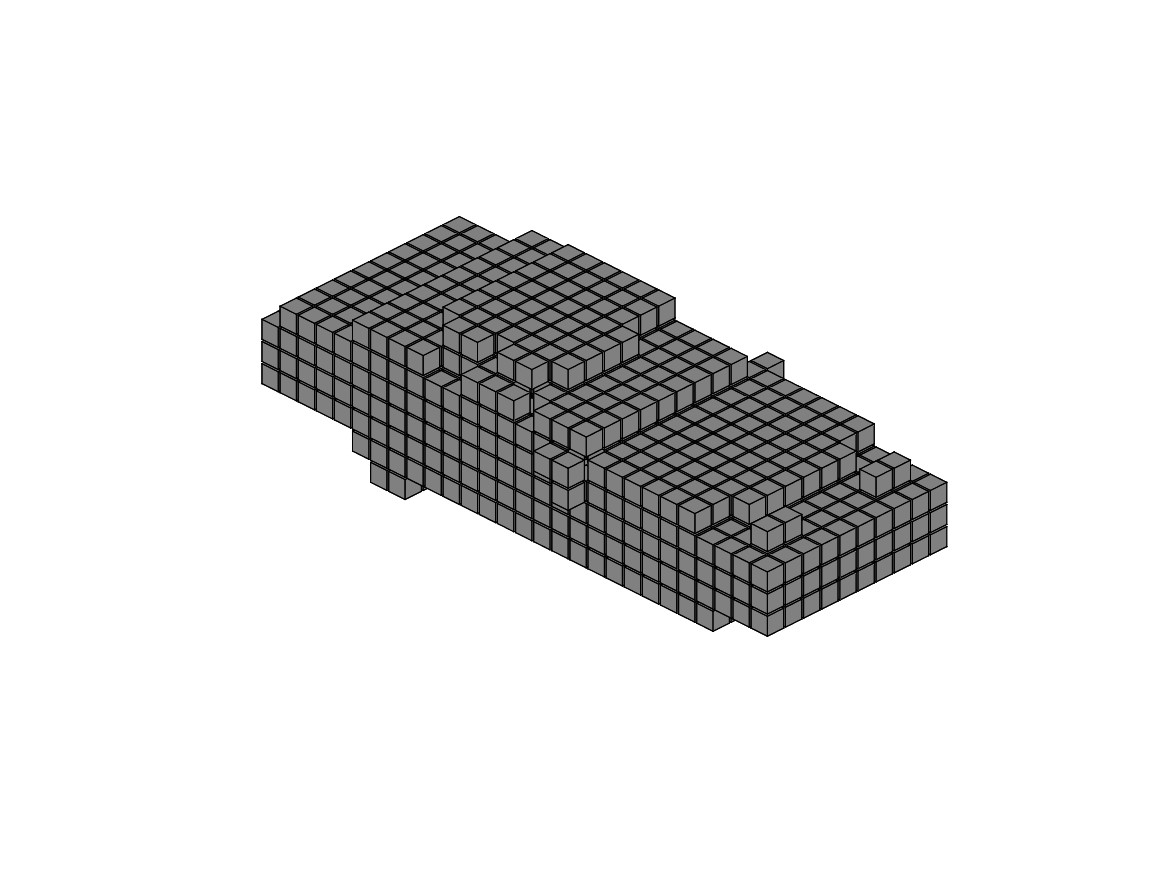
\includegraphics[height=2.5cm,trim={2cm 1cm 2cm 1cm},clip]{data/shapenet/1_output}};
    
    \node at (9, -3.5) {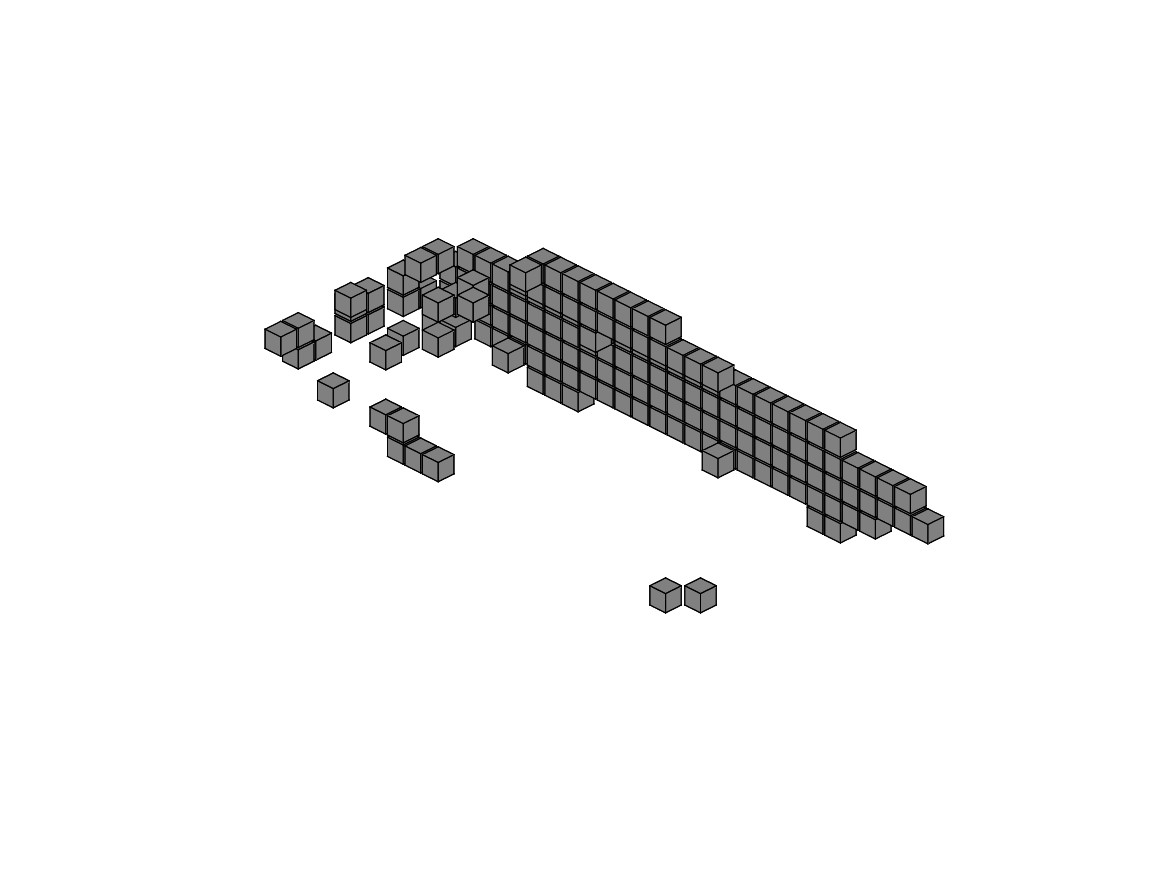
\includegraphics[height=2.5cm,trim={2cm 1cm 2cm 1cm},clip]{data/shapenet/1_input}};
    %\node at (9, -5.5) {\includegraphics[height=2.5cm]{data/shapenet/0_real_space}};
    
    \draw[->] (4,-1.5) -- (4, -2.5);
    \node at (4.4,-2) {(c)};
    
    \draw[->] (9,-1.5) -- (9, -2.5);
    \node at (9.4,-2) {(d)};
    
    \node at (-2,-4.7) {(e)};
    \draw[-,dashed] (-3,-5) -- (11,-5);
    
    \node[anchor=east] at (0.75,-6) {\footnotesize Voxelized Shape};
    \node[anchor=east] at (0.75,-7) {\footnotesize Filled Shape};

    \node[anchor=east] at (0.75,-8) {\footnotesize Voxelized Points};
    \node[anchor=east] at (0.75,-9) {\footnotesize Voxelized Free Space};

  \node[anchor=east] at (0.75,-10) {\footnotesize \begin{tabular}{r@{}}Distance Function\\for Points\end{tabular}};
    \node[anchor=east] at (0.75,-11) {\footnotesize \begin{tabular}{r@{}}Distance Function\\for Free Space\end{tabular}};

    \node[anchor=east] at (0.75,-13.25) {\footnotesize \begin{tabular}{r@{}}Signed Distance\\Function for Shape\end{tabular}};

    \node at (6,-6.5) {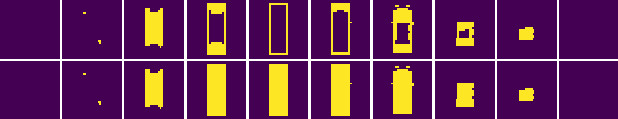
\includegraphics[width=10cm]{data/shapenet/0_output_slices}};
    \node at (6,-9.5) {\includegraphics[width=10cm]{data/shapenet/0_sdf_slices}};
    \node at (6,-12) {\includegraphics[width=10.8cm]{data/shapenet/colorbar}};
    \node at (6,-13.25) {\includegraphics[width=10cm]{data/shapenet/0_sdf_output_slices}};
    \node at (6,-14.1) {\includegraphics[width=10.8cm]{data/shapenet/sdf_colorbar}};
  \end{tikzpicture}
  % TODO short caption
  \caption{Illustration of the data generation process on an example from
  the ShapeNet dataset. The original triangular mesh is
  shown in the top left. In (a), it is first simplified using the approach outlined in
  Algorithm \ref{alg:data-hull}. The simplified mesh is rendered, (b), from
  a random viewpoint. The simplified mesh is then voxelized using triangle-box
  intersections, (c), and the rendered depth map is used to generate and voxelize
  the observations, (d). Finally, in (e), the corresponding signed distance
  functions are computed. The top two rows show the filling process of the voxelized
  mesh, the next four rows show the observed points and observed free space
  and the corresponding distance functions; the last row shows the
  signed distance function of the filled mesh. Each row shows 
  horizontal slices of the corresponding volumes, \ie heights $11 + i$ for $0 \leq i < 10$.}
  \label{fig:data-3d-process}
\end{figure}

\subsection{Mesh Pre-Processing and Voxelization}

We prefer to work with watertight meshes; for the 3D cuboids we have control
about this as we automatically generate the meshes. In the case of ShapeNet
this is problematic. In addition, ShapeNet may contain very complex models 
where we need to deal with up to $100000$ faces.
%\footnote{
%  We manually chose a subset of all car models in ShapeNet to
%  sort out models that could not automatically be scaled to $[0,1]^3$
%  or where the dominant orientation could not be automatically determined.
%}
Often, these models
contain a level of detail that we are not interested in as it will be
lost during voxelization, especially in low resolution. Therefore,
we decided to follow \cite{GueneyGeiger:2015}\footnote{
  \url{http://www.cvlibs.net/software/semi_convex_hull/}.
} and compute a so-called
semi-convex hull.

% TODO for if really bold!
\begin{algorithm}[t]
  \small
	\begin{algo}{Semi-Convex Hull}{
	\label{alg:data-hull}
	\qinput{triangular mesh $\mathcal{M}$}
	\qoutput{simplified mesh $\mathcal{M}^{(T)}$}
	}
	  draw sample points $\mathcal{P}$ from $\mathcal{M}$\\
	  compute convex hull $\mathcal{M}^{(0)} = (V^{(0)}, F^{(0)})$ of $\mathcal{M}$\\
	  remesh $\mathcal{M}^{(0)}$ using \cite{FuhrmannAckermannGoesele:2010}\\
		\qfor $t = 0$ \qto $T - 1$\\
		  \qif $\mathcal{M} \not\subseteq \Vol(V^{(t)})$\\
		    \qthen find smallest $\alpha > 0$ such that $P \subseteq \Vol((1 + \alpha)V^{(t)})$\\
		    $V^{(t)} := (1 + \alpha) V^{(t)}$\\
		    remesh $\mathcal{M}^{(t)}$ using \cite{FuhrmannAckermannGoesele:2010}\qfi\\
		  $V^{(t + 1)} = V^{(t)} - \gamma \nabla \mathcal{L}(V^{(t)})$\qrof\\
		\qreturn $\mathcal{M}^{(T)}$
	\end{algo}
	% TODO short caption
	\caption{The semi-convex hull algorithm used in \cite{GueneyGeiger:2015}
	to obtain watertight, simplified meshes. Details can be found in the text.}
\end{algorithm}

Algorithm \ref{alg:data-hull} first samples a set of points $\mathcal{P}$ from the
given mesh $\mathcal{M} = (V, F)$. Then, a convex hull is computed -- 
a standard problem in computational geometry, see
\cite{Cormen:2009} or \cite{DeBergCheongVanKreveldOvermars:2008}.
To reduce the number of initial vertices, the approach of
\cite{FuhrmannAckermannGoesele:2010} is used to remesh the
initial mesh. The remeshed convex hull, $\mathcal{M}^{(0)}$,  is then
iteratively refined by minimizing a loss
\begin{align}
  \mathcal{L}(V^{(t)}) = \sum_{v \in V^{(t)}} \min_{p \in \mathcal{P}} \|v - p\|_2^2 + \sum_{(i, j) \in E(F^{(t)})}\left(\|v_i - v_j\|_2^2 - \mu\right)
\end{align}
using gradient descent. Here, $\mu$ is the mean edge length
of the initial mesh $\mathcal{M}^{(0)}$. A problem with this formulation is
that at any iteration $t$, the mesh $\mathcal{M}^{(t)}$ might not
contain the point set $\mathcal{P}$ anymore. In this case,
the vertices are rescaled as $V^{(t)} := (1 + \alpha)V^{(t)}$ such that
$\mathcal{P} \subseteq \Vol(V^{(t)})$, \ie the point set
$\mathcal{P}$ is contained in the volume spanned by $V^{(t)}$
and the mesh $M^{(t)}$ is remeshed again. Results of simplification
are shown in Figure \ref{fig:data-simplification}.

\begin{figure}
  \centering
  \hspace*{-0.25cm}
  \begin{subfigure}[t]{0.24\textwidth}
    \includegraphics[height=2.5cm]{data/shapenet/simplification/119033fe083145e22f31600ac759c763}
  \end{subfigure}\hfill
  \begin{subfigure}[t]{0.24\textwidth}
    \includegraphics[height=2.5cm]{data/shapenet/simplification/109567d7d55b8fe515a520abec2f04dd}
  \end{subfigure}\hfill
  \begin{subfigure}[t]{0.24\textwidth}
    \includegraphics[height=2.5cm]{data/shapenet/simplification/1089cbe82dc0e72133d7c9e122eec9b6}
  \end{subfigure}\hfill
  \begin{subfigure}[t]{0.24\textwidth}
    \includegraphics[height=2.5cm]{data/shapenet/simplification/100c3076c74ee1874eb766e5a46fceab}
  \end{subfigure} \\ 
  
  \begin{subfigure}[t]{0.24\textwidth}
    \includegraphics[height=2.7cm]{data/shapenet/simplification/0028}
  \end{subfigure}\hfill
  \begin{subfigure}[t]{0.24\textwidth}
    \includegraphics[height=2.7cm]{data/shapenet/simplification/0011}
  \end{subfigure}\hfill
  \begin{subfigure}[t]{0.24\textwidth}
    \includegraphics[height=2.7cm]{data/shapenet/simplification/0010}
  \end{subfigure}\hfill
  \begin{subfigure}[t]{0.24\textwidth}
    \includegraphics[height=2.7cm]{data/shapenet/simplification/0002}
  \end{subfigure}
  
  % TODO short caption
  \caption{Illustration of the employed mesh simplification approach, \ie
  Algorithm \ref{alg:data-hull}, on manually selected examples from ShapeNet.
  These show the variety available in the dataset.}
  \label{fig:data-simplification}
\end{figure}

After obtaining simple, watertight meshes, voxelization is performed using
triangle-voxel intersection tests as \eg proposed in\cite{AkenineMoeller:2001}\footnote{
  We also use the corresponding code from \url{http://fileadmin.cs.lth.se/cs/Personal/Tomas_Akenine-Moller/code/}.
}. In practice we scale, translate and pad all models to $[0,1]^3$,
which is then subdivided into $H \times W \times D$ axis-aligned voxels.
For the car models, care has to be taken to avoid skewing the models during
scaling, translating and padding. Note that all axes are scaled equally and we may
consider slight random rotation, translation and scaling for data augmentation.

\subsection{Mesh Filling}
\label{sec:data-3d-filling}

% TODO appendix multi-resolution approach
In order to obtain proper occupancy grids, \ie also identify interior
voxels, we use a flood filling/connected components algorithm
\cite{Dillencourt:1992}\cite[Section~3.3]{Szeliski:2011}.
As we work with watertight meshes, interior and exterior of the shapes
are clearly separated. For low resolutions, \eg $32^3$, this approach
works very well.

\subsection{Mesh Rendering and Observation Voxelization}

For simplicity, we use an OpenGL based MatLab renderer to obtain depth images from the pre-processed meshes.
To this end, we use the code also used in \cite{GeigerWang:2015,GueneyGeiger:2015}\footnote{
  \url{http://www.cvlibs.net/software/librender/}
}. Using the camera parameters used by OpenGL, the pixels in the depth image can
be back-projected into 3D space. By thresholding the depth value,
we know which pixels correspond to points on the mesh surface. By controlling
the depth image resolution as well as focal length, we indirectly control
the sparsity of the obtained point cloud. Using ray tracing we can additionally
derive free space. The process is described in detail in the following.

\begin{definition}
  \label{def:data-2d-camera}
  A (simplified) 2D projective camera is a tuple $(\mathcal{K}, \mathcal{R}, t)$
  where
  \begin{align}
    \mathcal{K} = \left[\begin{matrix}
      f_u & 0 & u\\
      0 & f_v & v\\
      0 & 0 & 1\\
    \end{matrix}\right]
  \end{align}
  is the intrinsic camera matrix,
  $\mathcal{R} \in \mathbb{R}^{3 \times 3}$ is a rotation matrix and
  $t \in \mathbb{R}^3$ a translation vector. Here, $f_u$ and $f_v$ are focal lengths
  along horizontal and vertical direction, respectively,
  and $(u, v)^T$ defines the principal point of the 2D image -- implicitly
  also defining its resolution, $2u \times 2v$, assuming that $(u,v)^T$ represents the
  center pixel.
\end{definition}

% TODO precise dimensions, also for 2D
The overall projection matrix of a camera $(\mathcal{K}, \mathcal{R}, t)$ is given by
$\mathcal{P} = \mathcal{K} \left[\begin{matrix}\mathcal{R} & t\end{matrix}\right] \in \mathbb{R}^{3 \times 4}$
and defines the projection of point $p = (p_1, p_2, p_3, 1)^T$ in homogeneous coordinates
to the corresponding pixel
\begin{align}
  x = \left[\begin{matrix}
    \frac{\tilde{x}_1}{\tilde{x}_3}\\
    \frac{\tilde{x}_2}{\tilde{x}_3}\\
    1
  \end{matrix}\right]\quad\text{ with }\quad \tilde{x} = \mathcal{P} p.
\end{align}
The inverse projection is defined as
its pseudo-inverse \cite[Chapter~6]{HartleyZisserman:2006}:
\begin{align}
  \mathcal{P}^+ = (\mathcal{P}^T \mathcal{P})^{-1} \mathcal{P}^T \in \mathbb{R}^{4 \times 3}
\end{align}
The ray corresponding to a pixel $x$ in homogeneous coordinates, \ie
$x = (x_1, x_2, 1)^T$, can then be obtained as
\begin{align}
  r = \left[\begin{matrix}
    \frac{\tilde{r}_1}{\tilde{r}_4}\\
    \frac{\tilde{r}_2}{\tilde{r}_4}\\
    \frac{\tilde{r}_3}{\tilde{r}_4}\\
    1
  \end{matrix}\right]
  \quad\text{ with }\quad \tilde{r} = \mathcal{P}^+ x
\end{align}
The corresponding 3D point can be derived when knowing the depth $d$ corresponding
to the ray $r$:
\begin{align}
  p = \left[\begin{matrix}
    d\cdot \frac{r_1}{r_3}\\
    d\cdot \frac{r_1}{r_3}\\
    d
  \end{matrix}\right]
\end{align}
In practice, we can also work in the camera's coordinate system such that
$\mathcal{R} = I$ and $t = 0$. As a result, the inverse projection matrix simplifies to
$\mathcal{P}^+ = \mathcal{K}^{-1}$. Then, we capture the shapes in
different rotations around the (vertical) height axis -- corresponding to
different viewpoints of the camera. After back-projection,
ray-voxel intersection tests \cite{WilliamsBarrusMorleyShirley:2005}\footnote{
  \url{http://www.cs.utah.edu/~awilliam/box/}
} can be used to determine free space voxels and occupied voxels can be determined
using point-voxel intersection tests. We rotate and translate the observations
to $[0, 1]^3$ and use the exact same subdivision into $H \times W \times D$
axis-aligned voxels as before. This way, the observations are aligned with the
corresponding ground truth shapes. To obtain free space voxels, we only consider
rays to points on the corresponding shape. We refer to the result as partial
free space as we do not consider rays corresponding to points on the background.
This is reasonable as rays from background points cannot be used reliably
on real data, \eg on KITTI.

\subsection{Noise}

To simulate real conditions, we want to inject artificial noise.  As we will see on the
KITTI dataset, correctly simulating the Velodyne sensor and the corresponding noise is
not trivial. We manually inspected many samples from the KITTI dataset and decided
to define two noise parameters, $\lambda_{\text{hit}}$ and $\theta_{\text{ignore}}$.
The former defines an exponential distribution \cite[Chapter~11]{Bishop:2006}:

\begin{definition}
  Let $\epsilon \in \mathbb{R}$, $\epsilon \geq 0$, be a random variable.
  Then $\epsilon$ is distributed according to
  an exponential distribution, \ie $\epsilon \sim \Exp(\epsilon;\lambda)$, with 
  parameter $\lambda$ if the probability density function is given by
  \begin{align}
    p(\epsilon) = \lambda \exp(-\lambda \epsilon).
  \end{align}
\end{definition}

Following inverse transform sampling \cite[Chapter~11]{Bishop:2006},
we draw samples from this distribution using $u \sim U(0,1)$ and
\begin{align}
  \epsilon = \frac{-\ln u}{\lambda}.
\end{align}
For each pixel in the depth image, we sample an error value
$\epsilon \sim \Exp(\epsilon;\lambda_{\text{hit}})$ from an
exponential distribution and add the value to the actual depth value.
This is reasonable, as $\epsilon$ will always be non-negative and $p(\epsilon)$
decreases exponentially for rising $\epsilon$.
The probability $\theta_{\text{ignore}}$ defines how likely an observation
is to be ignored. In this case, the depth value of the corresponding pixel is
set to the maximum depth.

\subsection{Discussion}

\begin{figure}
  \centering 
  \begin{subfigure}[t]{0.425\textwidth}
    \vspace{0px}
    \includegraphics[width=6cm]{data/shapenet/hard/data_6_0}\\
    \hspace*{-0.25cm}\includegraphics[width=6.5cm]{data/shapenet/easy/colorbar_0}
  \end{subfigure}
  \begin{subfigure}[t]{0.2\textwidth}
    \vspace{0px}
    \includegraphics[width=3cm,trim={2cm 1cm 2cm 1cm},clip]{data/shapenet/hard/6_input_45}
  \end{subfigure}
  \begin{subfigure}[t]{0.2\textwidth}
    \vspace{0px}
    \includegraphics[width=3cm,trim={2cm 1cm 2cm 1cm},clip]{data/shapenet/hard/6_target_45}
  \end{subfigure}\\
  \begin{subfigure}[t]{0.425\textwidth}
    \vspace{0px}
    \includegraphics[width=6cm]{data/3d/hard/data_0_0}\\
    \hspace*{-0.25cm}\includegraphics[width=6.5cm]{data/3d/easy/colorbar_0}
  \end{subfigure}
  \begin{subfigure}[t]{0.2\textwidth}
    \vspace{0px}
    \includegraphics[width=3cm,trim={2cm 1cm 2cm 1cm},clip]{data/3d/hard/0_input_45}
  \end{subfigure}
  \begin{subfigure}[t]{0.2\textwidth}
    \vspace{0px}
    \includegraphics[width=3cm,trim={2cm 1cm 2cm 1cm},clip]{data/3d/hard/0_target_45}
  \end{subfigure}
  \vskip 6px
  % TODO short caption
  % TODO text
  \caption{Examples from the created datasets corresponding to a model from ShapeNet
  (top) and a cuboid (bottom). In both cases we show heights $8 + 2i$ for $0 \leq i < 8$,
  \ie horizontal slices, illustrating the
  observed points, the computed partial free space and the ground truth shape.
  Additionally, we show 3D visualizations of the observed points and the corresponding
  shape; both in voxelized form.}
  \label{fig:data-3d-examples}
\end{figure}

% TODO artifacts
Figure \ref{fig:data-simplification} illustrates the variety of car models covered.
In addition, the simplified meshes are shown; we want to note that
some meshes, \eg from the Humvee on the right, are quite complex and this
complexity is vastly reduced during simplification. However, this also
incurs some loss of detail which we accept as voxelization is performed in
low resolution anyway. Figure \ref{fig:data-3d-examples} shows the corresponding voxelizations
for both ShapeNet and the 3D cuboids dataset when using
$\lambda_{\text{hit}} = 50$, $\theta_{\text{ignore}} = 0.1$, and
$2u \times 2v = 24 \times 32$ as resolution for the depth image. The noise
can best be observed in the horizontal slices of the sown volumes
-- especially considering the ignored rays.
More examples can be found in Appendix~\ref{ch:appendix-data}.

\section{KITTI}
\label{sec:data-kitti}

% TODO real bounding boxes
%\begin{figure}
%  \centering
%  \begin{tikzpicture}
    
    % https://tex.stackexchange.com/questions/40840/put-a-node-behind-another-in-a-tikz-diagram
%    \begin{scope}[on background layer]
%      \node at (0, 0) {
%        \includegraphics[height=5cm]{data/kitti/snapshot_00_rect}
%      };
%    \end{scope}
    
%    \node[rectangle,minimum width=3cm,minimum height=1cm,draw=red!75] (rect) at (-2.5,-0.25){};
%    \node[rectangle,draw=red!75] (excerpt) at (-4, 2.5) {
%      \includegraphics[height=3cm]{data/kitti/snapshot_01_rect}
%    };
    
%    \draw[-,red!75] (rect.north west) -- (excerpt.south west);
%    \draw[-,red!75] (rect.north east) -- (excerpt.south east);
%  \end{tikzpicture}
%  \vskip 6px
  % TODO short caption
%  \caption{Illustration of the raw point cloud extracted from the first
%  city drive in KITTI,
%  \ie \lstinline!2011_09_26_drive_0001!. The provided 3D bounding box corners are
%  marked green and points within a bounding box are marked blue. The top image
%  shows the scene from bird's eye view.}
%  \label{fig:data-kitti}
%\end{figure}

% TODO image of point cloud with bounding boxes
The KITTI dataset
is a standard dataset and benchmark for a variety of computer vision tasks.
Beneath stereo image pairs, point clouds were captured from a moving vehicle
using a $360^\circ$ Velodyne LiDAR sensor\footnote{
  Details can be found in \cite{GeigerLenzUrtasun:2012} as well as in the corresponding
  manual at \url{http://www.velodynelidar.com/lidar/products/manual/HDL-64E\%20Manual.pdf0}.
}. An example of a captured point cloud is shown in Figure \ref{fig:introduction}.
Annotations
include -- among others -- 3D bounding boxes for all cars visible
on the image plane (\ie point clouds were not annotated in $360^\circ$).
As discussed in Chapter \ref{ch:problem}, we tackle shape completion of
an individual object. Therefore, we assume a 3D object detector to be given.
Due to the limited scope of this thesis, we use the provided ground truth 3D
bounding boxes for our experiments. These are first extracted, scaled and
the corresponding points are voxelized. Free space is then computed using
ray tracing.
%Both is discussed in detail in the following.

%\subsection{3D Bounding Boxes}
% TODO avoid e_bb if not needed.
% TODO character for extents/dimensions!
%The point cloud is provided relative to the sensor's center; the corresponding
%3D bounding boxes are specified by defining the translation of its center
%$t_{\text{bb}}$, the rotational angle around the vertical (height) axis expressed in
%terms of the derived rotation matrix $\mathcal{R}_{\text{bb}}$, and the
%dimensions, \ie extents, of the box $e_{\text{bb}}$
%in terms of width $e_{\text{bb},1}$, height $e_{\text{bb},2}$ and depth
%$e_{\text{bb},3}$.

\subsection{Point Cloud Voxelization}

Each ground truth 3D bounding box is provided in the form of its center,
\ie translation from the sensor's center, the extents in terms of width,
height and depth as well as the rotational angle along the (vertical)
height axis. For voxelization, the bounding boxes are rotated
to be axis aligned and then scaled to the unit cube, \ie $[0,1]^3$.
Again, we make sure to scale all axes equally such that the
observations do not get skewed.

\subsection{Free Space Voxelization}

To voxelize free space, we follow the same approach as before, \ie ray tracing.
Again, we consider partial free space as the Velodyne sensor has difficulties with
reflective and transparent surfaces. In particular we found that many
rays go through the annotated cars and hit points in the background. 
Considering partial free space, this effect is reduced by only tracing
rays that correspond to points within the 3D bounding box.
We then compute ray-box intersections between all rays and all voxels
using the same subdivision into voxels as used before to avoid errors.
Still, some points are prone to lie within the observed car -- \eg at the
height of the windows -- causing voxels to erroneously be labeled as
free space.

\subsection{Filtering}

\begin{figure}
  \centering  
  \vspace{-0.25cm}
  \begin{subfigure}[t]{0.425\textwidth}
    \vspace{0px}
    \includegraphics[width=6cm]{data/kitti/150_1500_30_3/data_0_0}\\
    \hspace*{-0.25cm}\includegraphics[width=6.5cm]{data/kitti/150_1500_30_3/colorbar_0}
  \end{subfigure}
  \begin{subfigure}[t]{0.2\textwidth}
    \vspace{0px}
    \includegraphics[width=3cm,trim={2cm 1cm 2cm 1cm},clip]{data/kitti/150_1500_30_3/0_input_45}
  \end{subfigure}
  \begin{subfigure}[t]{0.2\textwidth}
    \vspace{0px}
    \includegraphics[width=3cm,trim={2cm 1cm 2cm 1cm},clip]{data/kitti/150_1500_30_3/0_input_135}
  \end{subfigure}\\[-4px]
  \begin{subfigure}[t]{0.425\textwidth}
    \vspace{0px}
    \includegraphics[width=6cm]{data/kitti/150_1500_30_3/data_1_0}\\
    \hspace*{-0.25cm}\includegraphics[width=6.5cm]{data/kitti/150_1500_30_3/colorbar_0}
  \end{subfigure}
  \begin{subfigure}[t]{0.2\textwidth}
    \vspace{0px}
    \includegraphics[width=3cm,trim={2cm 1cm 2cm 1cm},clip]{data/kitti/150_1500_30_3/1_input_45}
  \end{subfigure}
  \begin{subfigure}[t]{0.2\textwidth}
    \vspace{0px}
    \includegraphics[width=3cm,trim={2cm 1cm 2cm 1cm},clip]{data/kitti/150_1500_30_3/1_input_135}
  \end{subfigure}
  
  % TODO short caption
  % TODO text
  \caption{Two examples as extracted from KITTI. Again, we show horizontal slices
  of the voxelized points and the corresponding free space together with 3D visualizations
  of the observed points and the corresponding shape.}
  \label{fig:data-kitti-examples}
\end{figure}

Using all the voxelized observations to learn shape completion is not
realistic within the scope of this thesis -- especially as many
observations contain only very few observed points and erroneous free space.
Therefore, we filtered the voxelized observations to obtain an easier
dataset. First, we require that at least
$n_{1,\min}$ points are observed and $n_{0, \min}$ voxels correspond
to free space:
\begin{align}
  \sum_{i = 1}^R \mathds{1}[x_i = 1] \overset{!}{>} n_{1,\min}\quad\text{ and }\quad\sum_{i = 1}^R \mathds{1}[x_i = 0] \overset{!}{>} n_{0,\min};
\end{align}
Second, we require the distance of the 3D bounding
box to the Velodyne sensor to be less than $t_{\max}$. In practice, the
three constraints ensure that the extracted dataset is manageable to tackle
in the course of this thesis. Higher difficulties can then
be obtained by lowering $n_{1,\min}$ and $n_{0,\min}$ and increasing $t_{\max}$,
respectively. The exact constraints and some statistics are provided in
Chapter \ref{ch:experiments} when conducting experiments on KITTI.

\subsection{Discussion}

Overall, it is fair to say that KITTI's Velodyne data exhibits several
distinct noise patterns -- that we also tried to model in our synthetic datasets.
The examples chosen in Figure \ref{fig:data-kitti-examples} were manually selected to
illustrate that some bounding boxes clearly depict cars. Still, even in this example,
we notice some artifacts. For example, due to noise and discretization, observed
points frequently lie inside the car. This is problematic as the corresponding
free space derived by ray tracing is partly invalid. We also notice that this 
happens more frequently at the height of the car's windows -- 
sometimes the Velodyne's rays hit other objects inside the
car instead, \eg seats. In Appendix \ref{ch:appendix-data}, we show further
examples.

  \chapter{Experiments}
\label{ch:experiments}

This section presents experimental results regarding the
approaches to shape completion discussed in Chapter \ref{ch:shape-inference}
on all datasets introduced in Chapter \ref{ch:data}. Not all of the discussed
formulations perform equally well. Originally, we first conducted experiments
on our synthetic 2D rectangle dataset, see Appendix \ref{ch:appendix-experiments}, 
and found that maximum likelihood (\ML), does not perform well. For clarity, we
only present experiments on our synthetic 3D datasets, \ie cuboids and cars from ShapeNet
\cite{ChangFunkhouserGuibasSavarese:2015}, as well as on real data, \ie 
KITTI \cite{GeigerLenzUrtasun:2012,GeigerLenzStillerUrtasun:2013}.
Overall, we consider variational auto encoders (\VAEs) for learning shape priors
and amortized maximum likelihood (\AML) as well as
extended variational auto-encoders (\EVAEs) for shape completion.
Due to space constraints, the presented experiments are complemented
by additional results in Appendix \ref{ch:appendix-experiments}.
We first discuss the experimental setup before discussing experiments
on 3D cuboids and cars as well as on KITTI.

\section{Experimental Setup}

% TODO early stopping
% TODO training
We implemented all discussed approaches in the Torch\footnote{
  \url{http://torch.ch/}.
} deep learning framework. The implementations can be understood as prototypes;
we did not optimize them with respect to runtime or memory consumption.
Data pre-processing and generation as well as evaluation was performed in Python
and C++ as described in Chapter \ref{ch:data}. For all experiments we use a resolution
of $H \times W \times D = 32^3$ and assume a uniform subdivision of $[0,1]$ into
$32^3$ voxels for voxelization. As already stated, we derive signed distance functions
from the corresponding occupancy grids using distance transforms. Details on the
artificially added noise as well as data augmentation is discussed in the corresponding
sections.
In the following we briefly describe the used architectures
and evaluation metrics.

\subsection{Architecture and Training}

The architectures used for our experiments are kept simple.
While we experimented with deeper and more complex architectures
including skip connections, residual units \cite{HeSun:2016} and
inception-based architectures \cite{SzegedyRabinovich:2015,SzegedyWojna:2016},
these changes had no significant influence.
We follow the architectures illustrated in Figures \ref{subfig:experiments-2d-architecture-vae}
and \ref{fig:shape-inference-evae} for \VAEs and \EVAEs, respectively.
Encoder and decoder both consist of four stages of convolutional
layers including batch normalization, $\ReLU$ non-linearity and max
pooling/nearest neighbor upsampling. We follow discussions
in the literature \cite{SzegedyWojna:2016}
and increase the width of the network (\ie the number of channels) whenever decreasing the
spatial size of the feature maps and use $3 \times 3 \times 3$ convolution kernels
with zero padding and non-overlapping $2 \times 2 \times 2$ windows for max pooling and
nearest neighbor upsampling. For $32 \times 32 \times 32$ we thus reduce the spatial
size to $2 \times 2 \times 2$ before computing the latent code.
For both \AML and \EVAE, the new encoders, \ie $z(x; w)$ and $q(z | x)$, are trained from
scratch but follow the architecture of the shape prior. In this case, the corresponding
generative model $p(y | z)$ is always kept fixed.
For \AML, we additionally remove the fully connected layer predicting
the variance of the latent code
to obtain a deterministic encoder. For \EVAE, the additional decoder $p(x | y)$
consists of seven convolutional stages including batch normalization and
$\ReLU$ non-linearities. When predicting occupancy, we use Sigmoid non-linearities;
for predicting signed distance functions we use the identity, \ie no non-linearity.
We refer to Appendix \ref{ch:appendix-experiments} for training details.

\subsection{Evaluation}
\label{sec:experiments-2d-evaluation}

For evaluation we resort to the absolute error between prediction
and ground truth for both representations, \ie occupancy and signed distance functions.
For a prediction
$y \in \mathbb{R}^{H \times W \times D}$ and ground truth
$y^* \in \mathbb{R}^{H \times W \times D}$ we average over all spatial dimensions:
\begin{align}
  \Abs(y, y^*) = \frac{1}{HWD} \sum_{i_1 = 1}^H \sum_{i_2 = 1}^W \sum_{i_3 = 1}^D \left|y_i - y^*_i\right|.
  \label{eq:experiments-2d-abs}
\end{align}
We always report the average on the validation set (or on batches during training).
We additionally use the absolute error after thresholding the predicted shapes,
\ie after obtaining proper occupancy grids. For occupancy grids, we threshold 
the predicted occupancy probabilities at $0.5$ and
for signed distance functions we threshold at $0$ (here, negative values correspond
to occupied voxels). These thresholds are also used for our 3D visualizations.
We refer to the absolute error after thresholding as $\AbsThr$. Overall,
the absolute error is easy to interpret,
\eg it provides a clear lower bound (which is $\Abs \geq 0$), and comparable
across datasets and methods.

Because the discussed approaches try to maximize the likelihood -- or the
corresponding evidence lower bound -- during training, we would also like
to consider the negative log-likelihood as measure.
However, we found the negative log-likelihood to be unsuited for evaluation.
First, the negative log-likelihood is harder to interpret as it strongly
depends on the model (\eg \VAE or \EVAE). In particular, besides the
reconstruction loss, all models also include (possibly weighted) prior terms
-- \eg in form of Kullback-Leibler divergences or the negative log-likelihood
corresponding to the prior $p(z)$. Furthermore, for \EVAE, the reconstruction loss does not
represent the objective we are actually trying to optimize for shape completion.
Second, across datasets, the negative log-likelihood depends on the number of
observed voxels. Thus, performance of the proposed shape completion approaches
cannot be compared to the reconstruction performance of the shape prior -- 
which would be a natural baseline.
Third, the negative log-likelihood on Bernoulli observations is inherently skewed
towards ``unsure'' predictions; meaning that the negative log-likelihood
prefers unsure predictions over very certain predictions with few mistakes
(see Appendix \ref{ch:appendix-experiments} for an example). This is
reasonable during training where we explicitly want to model uncertainty,
but hinders fair evaluation. Overall, we decided not to report any negative log-likelihoods.

\section{3D Example}
\label{sec:experiments-3d}

% TODO nicer tables
\begin{table}
  \centering
  {\footnotesize
  \renewcommand{\arraystretch}{1.1}
  \begin{tabularx}{\textwidth}{| X | c | c | c |}
    \hline
    & \Cub\easy & \Cub\moderate & \Cub\hard\\\hline
    Training Size (Prior/Inference) & \multicolumn{3}{c|}{$10000/10000$}\\\hline
    Validation Size & \multicolumn{3}{c|}{$1000$}\\\hline
    Resolution $H \times W \times D$ & \multicolumn{3}{c|}{$32 \times 32 \times 32$}\\\hline
    Resolution $2u \times 2v$ & $48 \times 64$ & \multicolumn{2}{c|}{$24 \times 32$}\\\hline
    Noise $\lambda_{\text{hit}}$ & $0$ & $50$ & $50$\\\hline
    Noise $\theta_{\text{ignore}}$ & $0$ & $0$ & $0.1$\\\hline
    Observed Voxels (Inference Training Set) & $1.43\%$ & $0.53\%$ & $0.48\%$\\\hline
    Free Space Voxels (Inference Training Set) & $10.73\%$ & $7.07\%$ & $8.32\%$\\\hline
    Occupied Voxels (Inference Training Set) & $16.24\%$ & $16.17\%$ & $16.21\%$\\\hline
  \end{tabularx}
  }
  \vskip 6px
  % TODO short caption
  \caption{Overview of the generated datasets. We created datasets of three
  difficulties, \easy, \moderate and \hard, which refer to increased noise
  and less observations. Details on the parameters are discussed
  in Section \ref{sec:data-3d}. Additionally, we report statistics such as the
  percentage of observed voxels, free space voxels and occupied voxels
  (of the ground truth shapes) over the training set used for shape inference.}
  \label{table:experiments-3d-datasets}
\end{table}

We start with experiments on our synthetic 3D cuboids dataset.
Here, we are able to present both quantitative and qualitative results
on a controlled, simple dataset. To this end, we created datasets of three difficulties
following the procedure in Chapter \ref{ch:data}:
\easy, \hard and \moderate with details in Table \ref{table:experiments-3d-datasets}.
With rising difficulty, less observations are provided and the underlying noise increases.
The \hard case is supposed to represent real conditions as found on KITTI.
Examples for all three difficulties can be found in Appendix \ref{ch:data}. In
Table \ref{table:experiments-3d-datasets} we additionally report some
basic statistics, \eg the percentage of occupied voxels to give an impression
of how trivial predictions would perform or the percentage of observed
and free space voxels to indicate what level of supervision is available.
We start with discussing the \VAE shape prior before proceeding to the problem
of shape completion. As we found \ML to perform poorly in the 2D case,
we exclude experiments on 3D data.

\subsection{Shape Prior}

\begin{figure}[t]
  \begin{subfigure}[t]{0.48\textwidth}
    \begin{tikzpicture}
      \begin{axis}[
          % https://tex.stackexchange.com/questions/68577/compiling-a-document-with-pgfplots-processing-only-every-x-th-data-point
          each nth point=2,
          filter discard warning=false,
          unbounded coords=discard,
          % https://tex.stackexchange.com/questions/13816/dimension-too-large-while-plotting-with-pgfplots
          %restrict y to domain=0:0.1,
          %restrict x to domain=0:250000,
          log ticks with fixed point,
          ymin=0,
          ymax=0.06,
          xmin=0,
          xmax=125000,
          %xticklabel={
          %  \pgfmathparse{\tick/1000}
          %  \pgfmathprintnumber{\pgfmathresult}k
          %},
          xtick={0,50000,100000},
          xticklabels={0,50k,100k},
          xticklabel style={
            /pgf/number format/fixed
          },
          scaled x ticks=false,
          yticklabel style={
            /pgf/number format/fixed
          },
          scaled y ticks=false,
          %x coord trafo/.code={\pgfmathparse{\pgfmathresult/1000}},
          %xticklabel=\pgfmathprintnumber{\tick}k,
          width=7.5cm,
          height=5cm,
          % https://tex.stackexchange.com/questions/48620/pgfplots-alignment-and-size-of-math-in-legend
          legend cell align=left,
        ]
        
        % https://tex.stackexchange.com/questions/276869/reading-an-unusual-coordinates-file-in-pgfplots
        \addplot +[mark=none] table[ignore chars={(,)},col sep=comma] {data/experiments/3d/vae_occ/easy_15/training_loss.txt};
        \addlegendentry{$\mathcal{L}_{\text{BCE}} + \KL$ (train)};
        \addplot +[mark=none] table[ignore chars={(,)},col sep=comma] {data/experiments/3d/vae_occ/easy_15/training_abs.txt};
        \addlegendentry{$\Abs$ (train)};
        
        \addplot +[mark=none] table[ignore chars={(,)},col sep=comma] {data/experiments/3d/vae_occ/easy_15/validation_loss.txt};
        \addlegendentry{$\mathcal{L}_{\text{BCE}} + \KL$ (val)};
        \addplot +[mark=none] table[ignore chars={(,)},col sep=comma] {data/experiments/3d/vae_occ/easy_15/validation_abs.txt};
        \addlegendentry{$\Abs$ (val)};
      \end{axis}
    \end{tikzpicture}
  \end{subfigure}\hfill
  \begin{subfigure}[t]{0.48\textwidth}
    \begin{tikzpicture}
      \begin{axis}[
          % https://tex.stackexchange.com/questions/68577/compiling-a-document-with-pgfplots-processing-only-every-x-th-data-point
          %each nth point=100,
          filter discard warning=false,
          unbounded coords=discard,
          % https://tex.stackexchange.com/questions/13816/dimension-too-large-while-plotting-with-pgfplots
          %restrict y to domain=0:0.1,
          %restrict x to domain=0:250000,
          %ymin=0,
          %ymax=0.4,
          xmin=0,
          xmax=125000,
          %xticklabel={
          %  \pgfmathparse{\tick/1000}
          %  \pgfmathprintnumber{\pgfmathresult}k
          %},
          xtick={0,50000,100000},
          xticklabels={0,50k,100k},
          xticklabel style={
            /pgf/number format/fixed
          },
          scaled x ticks=false,
          yticklabel style={
            /pgf/number format/fixed
          },
          scaled y ticks=false,
          %x coord trafo/.code={\pgfmathparse{\pgfmathresult/1000}},
          %xticklabel=\pgfmathprintnumber{\tick}k,
          width=7.5cm,
          height=5cm,
          % https://tex.stackexchange.com/questions/48620/pgfplots-alignment-and-size-of-math-in-legend
          legend cell align=left,
        ]
        
        \addplot +[mark=none] table[ignore chars={(,)},col sep=comma] {data/experiments/3d/vae_occ/easy_15/validation_mean.txt};
        \addlegendentry{$\overline{\mu}$ (val)};
        \addplot +[mark=none] table[ignore chars={(,)},col sep=comma] {data/experiments/3d/vae_occ/easy_15/validation_var.txt};
        \addlegendentry{$\exp\left(\frac{1}{2}\overline{l}\right)$ (val)};
        \addplot +[mark=none] table[ignore chars={(,)},col sep=comma] {data/experiments/3d/vae_occ/easy_15/validation_std.txt};
        \addlegendentry{$|1 - \sqrt{\Var[\mu]}|$ (val)};
      \end{axis}
    \end{tikzpicture}
  \end{subfigure}
  \caption{Training curves for a \VAE with $Q = 15$ trained on the 3D cuboids dataset. We show
  the training loss, \ie $\mathcal{L}_{\text{BCE}} + \KL$, on the training (train) and validation set (val)
  as well as the corresponding absolute error \Abs on the left. Statistics corresponding to the latent
  space, particularly, the average $\overline{\mu}$ of the predicted means and the corresponding 
  standard deviation $\sqrt{\Var[\mu]}$ as well as the average of the predicted standard
  deviations $\exp(\frac{1}{2} \overline{l})$ are shown on the right. For the latter we also
  refer to Equations \eqref{eq:shape-prior-monitor-mean-mean}, \eqref{eq:shape-prior-monitor-variance-mean}
  and \eqref{eq:shape-prior-monitor-mean-variance} for details.}
  \label{fig:experiments-3d-vae-t}
\end{figure}

\begin{figure}
  \centering
  \vspace{-0.25cm}
  \begin{tikzpicture}
    \node at (0, 1.1){
      \includegraphics[width=6cm]{experiments/3d/vae_occ/easy_15/results_0}
    };
    \node at (0, -1.1){
      \includegraphics[width=6cm]{experiments/3d/vae_occ/easy_15/results_1}
    };
    
    \draw[-,dashed] (3.25, -8) -- (3.25,3);
    
    \node at (6.5, 0){
      \includegraphics[width=6cm]{experiments/3d/vae_occ/easy_15/random}
    };
    
    \node at (10,0) {
      \includegraphics[height=5cm]{experiments/3d/vae_occ/easy_15/colorbar}
    };
    
    \node at (0, 3) {\begin{tabular}{c}reconstruction\\occupancy\end{tabular}};
    \node at (6.5, 3) {\begin{tabular}{c}random samples\\occupancy\end{tabular}};
    
    \draw[-,dashed] (-3.5, -2.5) -- (10, -2.5);
    
    %\node at (-3.5,-5) {
    %  \includegraphics[height=5cm]{experiments/3d/vae_occ_sdf/colorbar_0}
    %};
    
    \node at (0, -5){
      \includegraphics[width=6cm]{experiments/3d/vae_occ_sdf/easy_15/random_0_0}
    };
    
    %\draw[-,dashed] (3.25, -3) -- (3.25,3);
    
    \node at (6.5, -5){
      \includegraphics[width=6cm]{experiments/3d/vae_occ_sdf/easy_15/random_0_1}
    };
    
    \node at (10,-5) {
      \includegraphics[height=5cm]{experiments/3d/vae_occ_sdf/colorbar_1}
    };
   
    \node[rotate=90] at (-3.75, 0) {\begin{tabular}{c}predicting occupancy only\end{tabular}};
    \node[rotate=90] at (-3.75, -5) {\begin{tabular}{c}predicting occupancy and\\signed distance functions\end{tabular}};
   
    \node at (0, -8) {\begin{tabular}{c}random samples\\occupancy\end{tabular}};
    \node at (6.5, -8) {\begin{tabular}{c}random samples\\signed distance functions\end{tabular}};
  \end{tikzpicture}
  
  % TODO short caption
  \caption{Qualitative results for the trained \VAE shape prior with $Q = 15$ on the 3D cuboids dataset.
  We consider two models; one trained on occupancy only and one trained on both occupancy and
  signed distance functions. In the first case, we show reconstruction results on the left and
  random samples on the right. For the latter case, we show only random samples for both modalities.
  In all cases we show horizontal slices, \ie heights $8 + 2i$ for $0 \leq i < 8$. For random samples
  in the occupancy only case, we complement the results with 3D visualizations in Figure
  \ref{fig:experiments-3d-vae-qual-2}.}
  \label{fig:experiments-3d-vae-qual-1}
\end{figure}
\begin{figure}
  \centering
  \vspace{-0.25cm}
  \hspace*{-1cm}
  \begin{tikzpicture}
    \node at (0, 0) {
      \includegraphics[width=2.5cm,trim={2cm 1cm 2cm 1cm},clip]{experiments/3d/vae_occ/easy_15/0_random_15}
    };
    \node at (2.5, 0) {
      \includegraphics[width=2.5cm,trim={2cm 1cm 2cm 1cm},clip]{experiments/3d/vae_occ/easy_15/0_random_105}
    };
    
    \draw[-,dashed] (4,-1.5) -- (4, 1.5);
    
    \node at (5.5, 0) {
      \includegraphics[width=2.5cm,trim={2cm 1cm 2cm 1cm},clip]{experiments/3d/vae_occ/easy_15/5_random_15}
    };
    \node at (8, 0) {
      \includegraphics[width=2.5cm,trim={2cm 1cm 2cm 1cm},clip]{experiments/3d/vae_occ/easy_15/5_random_105}
    };
    
    \draw[-,dashed] (9.5,-1.5) -- (9.5, 1.5);
    
    \node at (11, 0) {
      \includegraphics[width=2.5cm,trim={2cm 1cm 2cm 1cm},clip]{experiments/3d/vae_occ/easy_15/2_random_15}
    };
    \node at (13.5, 0) {
      \includegraphics[width=2.5cm,trim={2cm 1cm 2cm 1cm},clip]{experiments/3d/vae_occ/easy_15/2_random_105}
    };
  \end{tikzpicture}
  \caption{Three random example of the \VAE shape prior with $Q = 15$ on the 3D cuboids dataset
  trained on occupancy only. In all three cases, we show two different viewpoints. We find that all
  three examples resemble cuboids. We also note that the \VAE has no difficulties predicting sharp corners
  and edges.}
  \label{fig:experiments-3d-vae-qual-2}
\end{figure}


For the shape prior, the size $Q$ of the latent space is crucial. We found that in
practice a suitable size can be determined by monitoring the training progress
of the \VAE for different sizes $Q$. For the following discussion, we determined
$Q = 15$ to be suitable and the corresponding training curves are shown
in Figure \ref{fig:experiments-3d-vae-t}.
%A comparison to $Q = 5$ and $Q = 30$ can be found in the appendix.
An important cue to judge $Q$
is the latent space, \ie whether learning the latent space converged. This is
usually be indicated by low predicted log-variances and the statistics of the predicted
means slowly resembling a unit Gaussian (\ie zero mean and unit variance).
Additionally, the obtained reconstruction error can be used as indicator. For $Q = 5$,
for example, the absolute error does not fall below $ \Abs \approx 0.04$.
Considering that, only
$~16.2\%$ of the voxels are occupied (\cf Table \ref{table:experiments-3d-datasets})
this error is still
very large. For $Q = 15$ and above, in contrast, the error reduces to $\Abs \approx 0.0054$ or lower.
Finally, we also consider random samples utilizing the generative model.
As can be seen in Figures \ref{fig:experiments-3d-vae-qual-1}
and \ref{fig:experiments-3d-vae-qual-2}, the random samples
look appropriate and mostly resemble cuboids.
Note that due to rotations, the cuboids might not appear rectangular when
showing horizontal slices of the corresponding volumes.
Overall, we did not exploit all possibilities regarding hyper parameters and
training time, but are satisfied with the obtained performance
using $Q = 15$.

On 2D examples, we realized that predicting both occupancy and signed
distance functions is beneficial compared to predicting signed distance functions
only. On 3D, we make a similar observation and show qualitative results
in Figure \ref{fig:experiments-3d-vae-qual-1}. Again, we use $Q = 15$,
and achieve an absolute error of $\Abs \approx 0.0064$ for occupancy and
$\Abs \approx 0.071$ for signed distance functions. After thresholding the
predicted representations to obtain occupancy grids (at $0.5$ for occupancy
probabilities and at $0$ for signed distance functions), the absolute error
drops to $\AbsThr \approx 0.0045$ and $\AbsThr \approx 0.0053$, respectively.
This means that both representations can be used to derive low-error
occupancy grids. Random samples also look suitable and clearly depict cuboids in
most cases; however, we find the samples to be slightly less sharp compared to
predicting occupancy only.
%For brevity, we include further qualitative results
%as well as training curves in Appendix \ref{ch:appendix-experiments}.

\subsection{Amortized Maximum Likelihood}
\label{sec:experiments-3d-aml}

\begin{figure}
  \centering
  \begin{subfigure}[t]{0.48\textwidth}
    \begin{tikzpicture}
      \begin{axis}[
          % https://tex.stackexchange.com/questions/68577/compiling-a-document-with-pgfplots-processing-only-every-x-th-data-point
          %each nth point=2,
          filter discard warning=false,
          unbounded coords=discard,
          % https://tex.stackexchange.com/questions/13816/dimension-too-large-while-plotting-with-pgfplots
          %restrict y to domain=0:0.1,
          %restrict x to domain=0:250000,
          ymin=0,
          ymax=0.12,
          xmin=0,
          xmax=31000,
          %xticklabel={
          %  \pgfmathparse{\tick/1000}
          %  \pgfmathprintnumber{\pgfmathresult}k
          %},
          xtick={0,15000,31000},
          xticklabels={0,15k,31k},
          xticklabel style={
            /pgf/number format/fixed
          },
          scaled x ticks=false,
          yticklabel style={
            /pgf/number format/fixed
          },
          scaled y ticks=false,
          %x coord trafo/.code={\pgfmathparse{\pgfmathresult/1000}},
          %xticklabel=\pgfmathprintnumber{\tick}k,
          width=7.5cm,
          height=5cm,
          % https://tex.stackexchange.com/questions/48620/pgfplots-alignment-and-size-of-math-in-legend
          legend cell align=left,
        ]
        
        % https://tex.stackexchange.com/questions/276869/reading-an-unusual-coordinates-file-in-pgfplots
        \addplot +[mark=none] table[ignore chars={(,)},col sep=comma] {data/experiments/3d/vae_occ_aml/moderate_15/training_loss.txt};
        \addlegendentry{$\mathcal{L}_{\text{BCE}} + \KL$ (train)};
        \addplot +[mark=none] table[ignore chars={(,)},col sep=comma] {data/experiments/3d/vae_occ_aml/moderate_15/training_abs.txt};
        \addlegendentry{$\Abs$ (train)};
        
        \addplot +[mark=none] table[ignore chars={(,)},col sep=comma] {data/experiments/3d/vae_occ_aml/moderate_15/validation_loss.txt};
        \addlegendentry{$\mathcal{L}_{\text{BCE}} + \KL$ (val)};
        \addplot +[mark=none] table[ignore chars={(,)},col sep=comma] {data/experiments/3d/vae_occ_aml/moderate_15/validation_abs.txt};
        \addlegendentry{$\Abs$ (val)};
      \end{axis}
    \end{tikzpicture}
  \end{subfigure}\hfill
  \begin{subfigure}[t]{0.48\textwidth}
    \begin{tikzpicture}
      \begin{axis}[
          % https://tex.stackexchange.com/questions/68577/compiling-a-document-with-pgfplots-processing-only-every-x-th-data-point
          %each nth point=100,
          filter discard warning=false,
          unbounded coords=discard,
          % https://tex.stackexchange.com/questions/13816/dimension-too-large-while-plotting-with-pgfplots
          %restrict y to domain=0:0.1,
          %restrict x to domain=0:250000,
          ymin=-0.2,
          ymax=0.5,
          xmin=0,
          xmax=31000,
          %xticklabel={
          %  \pgfmathparse{\tick/1000}
          %  \pgfmathprintnumber{\pgfmathresult}k
          %},
          xtick={0,15000,31000},
          xticklabels={0,15k,31k},
          xticklabel style={
            /pgf/number format/fixed
          },
          scaled x ticks=false,
          yticklabel style={
            /pgf/number format/fixed
          },
          scaled y ticks=false,
          %x coord trafo/.code={\pgfmathparse{\pgfmathresult/1000}},
          %xticklabel=\pgfmathprintnumber{\tick}k,
          width=7.5cm,
          height=5cm,
          % https://tex.stackexchange.com/questions/48620/pgfplots-alignment-and-size-of-math-in-legend
          legend cell align=left,
        ]
        
        \addplot +[mark=none] table[ignore chars={(,)},col sep=comma] {data/experiments/3d/vae_occ_aml/moderate_15/validation_mean.txt};
        \addlegendentry{$\overline{\mu}$ (val)};
        \addplot +[mark=none] table[ignore chars={(,)},col sep=comma] {data/experiments/3d/vae_occ_aml/moderate_15/validation_std.txt};
        \addlegendentry{$|1 - \sqrt{\Var[\mu]}|$ (val)};
      \end{axis}
    \end{tikzpicture}
  \end{subfigure}
  
  % TODO short caption
  \caption{Training curves for \AML using occupancy only and a \VAE prior
  with $Q = 15$ on the 3D cuboids dataset, specifically the \moderate case.
  Again, we show the quantities as in Figure \ref{fig:experiments-3d-vae-t}.
  We want to highlight that training takes place in the first few iterations;
  afterwards, training stagnates mostly.}
  \label{fig:experiments-3d-aml-t}
\end{figure}

\begin{figure}
  \centering
  \begin{tikzpicture}
    \begin{axis}[
        ybar stacked,
        % https://tex.stackexchange.com/questions/119887/remove-the-scientific-notation-which-is-unreasonable
        yticklabel style={
          /pgf/number format/fixed,
          /pgf/number format/precision=5
        },
        scaled y ticks=false,
        %enlargelimits=0.15,
        legend style={
          at={(1.01,1)},
          anchor=north west,
        },
        % https://tex.stackexchange.com/questions/48620/pgfplots-alignment-and-size-of-math-in-legend
        legend cell align=left,
        xtick={
          1, 2,
          3, 4, 5,
          6, 7, 8,
          9, 10, 11
        },
        xticklabels={
          \VAE, \VAE occ+sdf,
          \AML\\\easy, \AML\\\moderate, \AML \\\hard,
          \EVAE\\\easy, \EVAE\\\moderate, \EVAE\\\hard,
          \AML occ+sdf\\\easy, \AML occ+sdf\\\moderate, \AML occ+sdf\\\hard
        },
        x tick label style={text width=1.5cm,align=right},
        ymin=0,
        width=12.5cm,
        height=4cm,
        % https://tex.stackexchange.com/questions/271027/pgfplots-how-to-rotate-extra-x-tick-labels
        x tick label style={
          rotate=90,
          anchor=east,
        },
        enlarge x limits=0.05,
        % https://tex.stackexchange.com/questions/47882/formatting-a-pgfplot-graph-thicker-bars-and-total-width
        %bar width=8,
      ]
        
      % AbsThr
      \addplot +[bar shift=-.2cm] coordinates {
        (1, 0.00384198)
        (2, 0.00453785)
        (3, 0.03217211)
        (4, 0.03567748)
        (5, 0.04434539)
        %
        (6, 0.03876815)
        (7, 0.05154616)
        (8, 0.07254225)
        %
        (9, 0.04437874)
        (10, 0.05507257)
        (11, 0.0500495)
      };
      \addlegendentry{\AbsThr (occ)}
      % Abs
      \addplot +[bar shift=-.2cm] coordinates {
        (1, 0.00155) % 0.00539829)
        (2, 0.001953) % 0.00649281)
        (3, 0.000155) % 0.03232507)
        (4, 0.000218) % 0.03588854)
        (5, 0.000445) % 0.04479165)
        %
        (6, 0.00072) % 0.03942102)
        (7, 0.0003) % 0.05189751)
        (8, 0.00031) % 0.07285957)
        %
        (9, 0.0002) % 0.04457945)
        (10, 0.00016) % 0.05523896)
        (11, 0.00019) % 0.05023721)
      };
      \addlegendentry{\Abs (occ)}
      
      % --
      \resetelevenstackedplots
      
      % AbsThr
      \addplot +[bar shift=+.2cm] coordinates {
        (1, 0)
        (2, 0.00534606)
        (3, 0)
        (4, 0)
        (5, 0)
        %
        (6, 0)
        (7, 0)
        (8, 0)
        %
        (9, 0.04459624)
        (10, 0.05582422)
        (11, 0.05130592)
      };
      \addlegendentry{\AbsThr (sdf)}
      % Abs
      \addplot +[bar shift=+.2cm] coordinates {
        (1, 0)
        (2, 0.06582) % 0.07112682)
        (3, 0)
        (4, 0)
        (5, 0)
        %
        (6, 0)
        (7, 0)
        (8, 0)
        %
        (9, 0.17411) % 0.21871304)
        (10, 0.21636) % 0.27216289)
        (11, 0.2225) % 0.27388566)
      };
      \addlegendentry{\Abs (sdf)}
    \end{axis}
  \end{tikzpicture}
  
  % TODO short caption
  \caption{Absolute error \Abs and its thresholded variant \AbsThr, \ie
  the absolute error on thresholded predictions,
  for a comparison between the \VAE prior, \AML and \EVAE on occupancy only
  and \AML predicting both occupancy and signed distance functions (indicated as occ+sdf).
  In each case, the left bar represents results on occupancy; the right bar
  corresponds to results on signed distance functions (if applicable). The comparison
  to the \VAE prior provides a possible lower bound on the performance.}
  \label{fig:experiments-3d-aml-abs}
\end{figure}

\begin{figure}
  \centering
  \vskip -0.25cm
  \begin{tikzpicture}    
    \node at (0, 0){
      \includegraphics[width=6cm]{experiments/3d/vae_occ_aml/moderate_15/results_0}
    };
    \node at (0, -2.75) {
      \includegraphics[width=6cm]{experiments/3d/vae_occ_aml/inference_statistics_05}
    };
    \node at (0, -5.25){
      \includegraphics[width=6cm]{experiments/3d/vae_occ_aml/hard_15_statistics_05/results_0}
    };
    \node at (0, -9.75){
      \includegraphics[width=6cm]{experiments/3d/vae_evae/hard_15_statistics/results_0}
    };
    
    %\draw[-,dashed] (3.25, -3) -- (3.25,3);
    
    \node at (6.5, 0){
      \includegraphics[width=6cm]{experiments/3d/vae_occ_aml/moderate_15/results_1}
    };
    \node at (6.5, -2.75) {
      \includegraphics[width=6cm]{experiments/3d/vae_occ_aml/inference_statistics_05}
    };
    \node at (6.5, -5.25){
      \includegraphics[width=6cm]{experiments/3d/vae_occ_aml/hard_15_statistics_05/results_1}
    };
    \node at (6.5, -9.75){
      \includegraphics[width=6cm]{experiments/3d/vae_evae/hard_15_statistics/results_1}
    };
    
    \node at (10,0) {
      \includegraphics[height=4.25cm]{experiments/3d/vae_occ/easy_15/colorbar}
    };
   
    \draw[-,dashed] (-3.5,-2.125) -- (10,-2.125);
    \draw[-,dashed] (-3.5,-7.5) -- (10,-7.5);
    
    \node[rotate=90] at (-4, 0) {\begin{tabular}{c}\AML\\\moderate\end{tabular}};
    \node[rotate=90] at (-4, -4.25) {\begin{tabular}{c}\AML\\\hard\end{tabular}};
    \node[rotate=90] at (-4, -9.75) {\begin{tabular}{c}\EVAE\\\hard\end{tabular}};
    
  \end{tikzpicture}
  \vskip 6px
  
  % TODO short caption
  \caption{Qualitative results for \AML on the 3D cuboids dataset with a \VAE
  prior and $Q = 15$. We
  show results on \moderate and \hard difficulties in comparison with \EVAE.
  In all cases we show
  horizontal slices of the volumes, \ie heights $8 + 2i$ for $0 \leq i < 8$,
  for two samples samples,
  each showing the observed points, the partial free space, the target shape
  as well as the predicted shape and
  the corresponding error. For \AML and the hard case we additionally
  illustrate the weights $\rho_i$ that
  were used for both \AML and \EVAE.}
  \label{fig:experiments-3d-aml-qual-1}
\end{figure}
\begin{figure}
  \centering
  \vskip -0.25cm
  \begin{tikzpicture}    
    \node at (0, 0){
      \includegraphics[width=6cm]{experiments/3d/vae_occ_sdf_aml/hard_15_statistics/results_0_0}
    };
    \node at (0, -4){
      \includegraphics[width=6cm]{experiments/3d/vae_occ_sdf_aml/hard_15_statistics/results_1_0}
    };
    
    %\draw[-,dashed] (3.25, -3) -- (3.25,3);
    
    \node at (6.5, 0){
      \includegraphics[width=6cm]{experiments/3d/vae_occ_sdf_aml/hard_15_statistics/results_0_1}
    };
    \node at (6.5, -4){
      \includegraphics[width=6cm]{experiments/3d/vae_occ_sdf_aml/hard_15_statistics/results_1_1}
    };
    
    \node at (10,0) {
      \includegraphics[height=4.25cm]{experiments/3d/vae_occ_sdf_aml/colorbar_1}
    };
    
    \node at (-3.5,0) {
      \includegraphics[height=4.25cm]{experiments/3d/vae_occ_sdf_aml/colorbar_0}
    };
    
    \node at (0, 2.25) {occupancy};
    \node at (6.5, 2.25) {signed distance function};
    
  \end{tikzpicture}
  \vskip 6px
  
  % TODO short caption
  \caption{Qualitative results for \AML using a \VAE prior with $Q = 15$ trained on both
  occupancy and signed distance functions. Results correspond to the \hard case.
  We show two samples and both modalities. In all
  cases we show horizontal slices as in Figure \ref{fig:experiments-3d-aml-qual-1}
  corresponding to the observed points, the partial free space, the target shape as well as the
  predicted shape and its error. We selected two examples illustrating that 
  the model resorts to blob-like ``standard'' shapes.}
  \label{fig:experiments-3d-aml-qual-2}
\end{figure}



For \AML, we mainly present experiments on \moderate and \hard difficulties
as we found that \AML performs very well on \moderate difficulty.
%However,
%we provide additionally qualitative results for all cases in the appendix.
First of all, we note that the weight $\kappa$ on the negative log-likelihood of the prior, \ie
$- \ln p(z)$, is crucial for successful training. 
Figure \ref{fig:experiments-3d-aml-t} shows training curves for the \moderate case
when using $\kappa = 15$. Overall, the network achieves an absolute error of
$\Abs \approx 0.036$. If the weight $\kappa$ would not be large enough,
the network would quickly deviate from the unit Gaussian prior.
This can be observed
when monitoring the latent space, \ie the observed statistics $\sqrt{\Var[\mu]}$ and $\overline{\mu}$
deviate significantly from the unit Gaussian prior. If $\kappa$ is chosen too large, the prior
``collapses'', \ie $\sqrt{\Var[\mu]}$ approaches zero. If weighted
correctly, the prior takes care of enforcing the unit Gaussian in the first few iterations.
We found that matching the prior becomes important as a big portion of learning
takes place in the early iterations. This can also be seen in Figure
\ref{fig:experiments-3d-aml-t}; it seems that \AML needs only few epochs to
``learn'' inference.
Experimentally, we found that $\kappa = 15$ performs
well for the \moderate case, however, $\kappa = 30$ is necessary for the \hard case.
Unfortunately, we did not find any rule of thumb for setting $\kappa$ but needed to
resort to trial and error.
Overall, we find that training \AML gets is tricky in 3D;
experimenting with hyper-parameters becomes more important.
% TODO anneal \kappa

Figure \ref{fig:experiments-3d-aml-abs} compares prior performance with
the obtained absolute errors on \easy, \moderate and \hard difficulties.
Qualitative results for the \moderate case can be found
in Figure \ref{fig:experiments-3d-aml-qual-1}. \AML performs reasonably well
on \moderate difficulty. However, we found performance to be strongly
influenced by the noisy free space observations in the \hard case. Especially
the ignored rays cause problems. After closer investigation we
resorted to a simple approach to avoid these difficulties: we weight observations
$x_i = 0$ corresponding to free space by
\begin{align}
  \rho_i = 1 - \frac{\sum_{m = 1}^M y_{m,i}}{m},\quad \mathcal{Y} = \{y_m\}_{m = 1}^M \subseteq \{0,1\}^R.
  \label{eq:experiments-3d-weights}
\end{align}
The weight $\rho_i$ can be interpreted as free space statistics, \ie the likelihood that
voxel $i$ is not occupied over the prior training set. This concept is also illustrated
in Figure \ref{fig:experiments-3d-aml-qual-1}. We additionally experimented with using
$\rho_i^\lambda$, $\lambda \in (0,1)$ and determined $\lambda = 0.5$ to work well.
As a result, we are able to obtain nearly equal performance on \moderate
and \hard difficulties. Overall, this discussion also shows
the influence of individually weighting voxels in order to cope noisy observations.
    
Figure \ref{fig:experiments-3d-aml-abs} also shows results obtained
when predicting both occupancy and signed distance functions. The corresponding
qualitative results for the \hard can be found in Figure
\ref{fig:experiments-3d-aml-qual-2}. We found that in both the \moderate and
the \hard case, the predicted shapes are slightly larger than the target
shapes. Specifically, the model appears to resort to
``standard'', blob-like shapes which be close to a mean shape.
We already now that learning and predicting signed distance
functions is harder compared to occupancy only. The blob-like predictions
could also be explained by choosing the weight $\kappa$ too large, implicitly
constraining the model to shapes close to the mean shape. 
Unfortunately, an extensive investigation and hyper-parameter tuning was not
possible within the limited time-frame of this thesis.

\subsection{Extended Variational Auto-Encoder}

For the \EVAE, we obtain similar results as presented above, see
Figure \ref{fig:experiments-3d-aml-abs}. For example,
in the \easy case, an absolute error \Abs of $\sim 0.034$ is achieved --
this is only slightly worse than \AML. For the \moderate and \hard cases,
errors of $\sim 0.042$ and $\sim 0.057$ are achieved. This is worse than
\AML; however, we also note that we did not spend as much time
tuning hyper parameters and we might have under-estimating
required training time which is more relevant for the \EVAE as it includes
significantly more parameters.
We also note that the observed performance is in contrast to the
2D case, see Appendix \ref{ch:appendix-experiments}, where \EVAE slightly
outperformed \AML which also indicates that training time is relevant
-- in the 2D case, it seems, we allocated enough training time.
For the \hard case, examples can be found in Figure \ref{fig:experiments-3d-aml-qual-1}.
We can also see that \AML and \EVAE give very similar results, apart from the
fact that \EVAE slightly under-estimates the true cuboids' size. However, this is not surprising
as both approaches optimize a similar objective, only that it is wrapped in a Kullback-Leibler
divergence in the case of \EVAE. We intend to perform further experiments regarding
\EVAE in future work; however, given the provided evidence, we prefer \AML
due to lower training times and slightly better performance.

\subsection{Discussion}

First of all, we find that both the shape prior, \ie a \VAE, as well as the shape inference
models are hard to train on 3D data. Tuning hyper-parameters is important and
made difficult by the long training times, even in low resolutions such as $32^3$.
Specifically, we found that enforcing the shape prior is crucial. For \AML, for example,
we increased the weight on the negative log-likelihood $- \ln p(z)$ in order to obtain
reasonable results. Additionally, to cope with the \hard case, we weighted
free space voxels individually by their likelihood to actually correspond to free space
on the prior training set.
Overall, we demonstrated that
\VAEs are able to learn appropriate shape priors using both occupancy and signed distance functions.
Regarding shape completion, we showed that both \AML and \EVAE give reasonable
performance while \AML performs slightly better than \EVAE.
We also found that \AML and \EVAE give very similar results -- which is reasonable
considering the theoretic background. In the end, we are satisfied by the presented experiments
and proceed to the more complicated ShapeNet dataset.

\section{ShapeNet}

ShapeNet \cite{ChangFunkhouserGuibasSavarese:2015} is our first dataset
comprising realistic objects, in particular cars.
Later, ShapeNet will also be used to train the shape prior for shape
completion on KITTI \cite{GeigerLenzUrtasun:2012,GeigerLenzStillerUrtasun:2013}.
We first manually discarded
$262$ of the $3514$ simplified meshes that could not be automatically scale
and rotated to $[0,1]^3$ for further processing. We split the remaining models
into two training sets -- for prior and inference -- and a validation set
corresponding to the fractions $0.45:0.45:0.1$. On each model, we apply seven
random transformations including slight scaling, rotation and
translation to the meshes; additionally,
we flip every variant. Overall, we obtain the datasets outlined
in Table \ref{table:experiments-shapenet-datasets}; examples can be found
in Appendix \ref{ch:appendix-data}.

\begin{table}
  \centering
  {\footnotesize
  \renewcommand{\arraystretch}{1.1}
  \begin{tabularx}{\textwidth}{| X | c | c | c |}
    \hline
    & \Cub\easy & \Cub\moderate & \Cub\hard\\\hline
    Training Size (Prior/Inference) & \multicolumn{3}{c|}{$20496/20496$}\\\hline
    Validation Size & \multicolumn{3}{c|}{$4550$}\\\hline
    Resolution $H \times W \times D$ & \multicolumn{3}{c|}{$32 \times 32 \times 32$}\\\hline
    Resolution $2u \times 2v$ & $48 \times 64$ & \multicolumn{2}{c|}{$24 \times 32$}\\\hline
    Noise $\lambda_{\text{hit}}$ & $0$ & $50$ & $50$\\\hline
    Noise $\theta_{\text{ignore}}$ & $0$ & $0$ & $0.075$\\\hline
    Observed Voxels & $0.62\%$ & $0.31\%$ & $0.304\%$\\\hline
    Free Space Voxels & $3.91\%$ & $3.75\%$ & $4.37\%$\\\hline
    Observed Voxels & $5.54\%$ & $5.51\%$ & $5.52\%$\\\hline
  \end{tabularx}
  }
  \vskip 6px
  % TODO short caption
  \caption{Overview of the generated datasets. We created datasets of three
  difficulties, \easy, \moderate and \hard, which refer to increased noise
  and less observations. Details on the parameters are discussed
  in Section \ref{sec:data-3d}.}
  \label{table:experiments-shapenet-datasets}
\end{table}

\subsection{Shape Prior}

\begin{figure}[b]
  \centering
  \begin{subfigure}[t]{0.48\textwidth}
    \begin{tikzpicture}
      \begin{axis}[
          % https://tex.stackexchange.com/questions/68577/compiling-a-document-with-pgfplots-processing-only-every-x-th-data-point
          each nth point=4,
          filter discard warning=false,
          unbounded coords=discard,
          % https://tex.stackexchange.com/questions/13816/dimension-too-large-while-plotting-with-pgfplots
          %restrict y to domain=0:0.1,
          %restrict x to domain=0:250000,
          log ticks with fixed point,
          ymin=0,
          ymax=0.05,
          xmin=0,
          xmax=250000,
          %xticklabel={
          %  \pgfmathparse{\tick/1000}
          %  \pgfmathprintnumber{\pgfmathresult}k
          %},
          xtick={0,50000,100000,150000,200000,250000},
          xticklabels={0,50k,100k,150k,200k,250k},
          xticklabel style={
            /pgf/number format/fixed
          },
          scaled x ticks=false,
          yticklabel style={
            /pgf/number format/fixed
          },
          scaled y ticks=false,
          %x coord trafo/.code={\pgfmathparse{\pgfmathresult/1000}},
          %xticklabel=\pgfmathprintnumber{\tick}k,
          width=7.5cm,
          height=5cm,
          % https://tex.stackexchange.com/questions/48620/pgfplots-alignment-and-size-of-math-in-legend
          legend cell align=left,
        ]
        
        % https://tex.stackexchange.com/questions/276869/reading-an-unusual-coordinates-file-in-pgfplots
        \addplot +[mark=none] table[ignore chars={(,)},col sep=comma] {data/experiments/shapenet/vae_occ/easy_15_long/training_loss.txt};
        \addlegendentry{$\mathcal{L}_{\text{BCE}} + \KL$ (train)};
        \addplot +[mark=none] table[ignore chars={(,)},col sep=comma] {data/experiments/shapenet/vae_occ/easy_15_long/training_abs.txt};
        \addlegendentry{$\Abs$ (train)};
        
        \addplot +[mark=none] table[ignore chars={(,)},col sep=comma] {data/experiments/shapenet/vae_occ/easy_15_long/validation_loss.txt};
        \addlegendentry{$\mathcal{L}_{\text{BCE}} + \KL$ (val)};
        \addplot +[mark=none] table[ignore chars={(,)},col sep=comma] {data/experiments/shapenet/vae_occ/easy_15_long/validation_abs.txt};
        \addlegendentry{$\Abs$ (val)};
      \end{axis}
    \end{tikzpicture}
  \end{subfigure}\hfill
  \begin{subfigure}[t]{0.48\textwidth}
    \begin{tikzpicture}
      \begin{axis}[
          % https://tex.stackexchange.com/questions/68577/compiling-a-document-with-pgfplots-processing-only-every-x-th-data-point
          each nth point=2,
          filter discard warning=false,
          unbounded coords=discard,
          % https://tex.stackexchange.com/questions/13816/dimension-too-large-while-plotting-with-pgfplots
          %restrict y to domain=0:0.1,
          %restrict x to domain=0:250000,
          %ymin=0,
          ymax=0.5,
          xmin=0,
          xmax=250000,
          %xticklabel={
          %  \pgfmathparse{\tick/1000}
          %  \pgfmathprintnumber{\pgfmathresult}k
          %},
          xtick={0,50000,100000,150000,200000,250000},
          xticklabels={0,50k,100k,150k,200k,250k},
          xticklabel style={
            /pgf/number format/fixed
          },
          scaled x ticks=false,
          yticklabel style={
            /pgf/number format/fixed
          },
          scaled y ticks=false,
          %x coord trafo/.code={\pgfmathparse{\pgfmathresult/1000}},
          %xticklabel=\pgfmathprintnumber{\tick}k,
          width=7.5cm,
          height=5cm,
          % https://tex.stackexchange.com/questions/48620/pgfplots-alignment-and-size-of-math-in-legend
          legend cell align=left,
        ]
        
        \addplot +[mark=none] table[ignore chars={(,)},col sep=comma] {data/experiments/shapenet/vae_occ/easy_15_long/validation_mean.txt};
        \addlegendentry{$\overline{\mu}$ (val)};
        \addplot +[mark=none] table[ignore chars={(,)},col sep=comma] {data/experiments/shapenet/vae_occ/easy_15_long/validation_var.txt};
        \addlegendentry{$\exp\left(\frac{1}{2}\overline{l}\right)$ (val)};
        \addplot +[mark=none] table[ignore chars={(,)},col sep=comma] {data/experiments/shapenet/vae_occ/easy_15_long/validation_std.txt};
        \addlegendentry{$|1 - \sqrt{\Var[\mu]}|$ (val)};
      \end{axis}
    \end{tikzpicture}
  \end{subfigure}
  \vskip 6px
  
  % TODO short caption
  \caption{Training curves for a \VAE with $Q = 15$ trained on occupancy only
  on the ShapeNet dataset. In comparison with Figure \ref{fig:experiments-3d-vae-t},
  we plot training (train) and validation (val) loss, \ie $\mathcal{L}_{\text{BCE}} + \KL$,
  the corresponding absolute error \Abs as well as latent space statistics
  $\overline{\mu}$, $\sqrt{\Var[\mu]}$ and $\exp(\frac{1}{2} \overline{l})$
  corresponding to the average of the precited means, the corresponding standard
  deviation and the average of the predicted standard deviations.}
  \label{fig:experiments-shapenet-vae-t}
\end{figure}

% TODO replace by long version
\begin{figure}
  \centering
  \begin{tikzpicture}    
    %\node at (-3.5,0) {
    %  \includegraphics[height=5cm]{experiments/3d/vae_occ_sdf/colorbar_0}
    %};
    
    \node at (0, 1.2){
      \includegraphics[width=6cm]{experiments/shapenet/vae_occ/easy_15_long/results_1}
    };
    \node at (0, -1.2){
      \includegraphics[width=6cm]{experiments/shapenet/vae_occ/easy_15_long/results_2}
    };
    
    \node at (6.5, 0){
      \includegraphics[width=6cm]{experiments/shapenet/vae_occ/easy_15_long/random_0}
    };
    
    \node at (0, 3) {\begin{tabular}{c}reconstruction\\occupancy\end{tabular}};
    \node at (6.5, 3) {\begin{tabular}{c}random samples\\occupancy\end{tabular}};
    
    \draw[-,dashed] (-3.5, -2.5) -- (10, -2.5);
    
    \node at (10, 0) {
      \includegraphics[height=4.2cm]{experiments/3d/vae_occ/easy_15/colorbar}
    };
    
    %\node at (-3.5,-5) {
    %  \includegraphics[height=5cm]{experiments/3d/vae_occ_sdf/colorbar_0}
    %};
    
    \node at (0, -5){
      \includegraphics[width=6cm]{experiments/shapenet/vae_occ_sdf/easy_15/random_0_0}
    };
    
    %\draw[-,dashed] (3.25, -3) -- (3.25,3);
    
    \node at (6.5, -5){
      \includegraphics[width=6cm]{experiments/shapenet/vae_occ_sdf/easy_15/random_0_1}
    };
    
    \node at (10,-5) {
      \includegraphics[height=5cm]{experiments/3d/vae_occ_sdf/colorbar_1}
    };
    
    \node[rotate=90] at (-3.75, 0) {\begin{tabular}{c}predicting occupancy only\end{tabular}};
    \node[rotate=90] at (-3.75, -5) {\begin{tabular}{c}predicting occupancy and\\signed distance functions\end{tabular}};
        
    \node at (0, -8) {\begin{tabular}{c}random samples\\occupancy\end{tabular}};
    \node at (6.5, -8) {\begin{tabular}{c}random samples\\signed distance functions\end{tabular}};
  \end{tikzpicture}
  \caption{Qualitative results considering reconstruction and random samples
  for a \VAE prior, $Q = 15$, learned on ShapeNet using occupancy only (top) and
  both occupancy and signed distance functions. In the latter case we only show
  random samples in both modalities. For reconstructions we show the target shape,
  the prediction as well as the corresponding error. In all cases we resort to
  showing horizontal slices as done before. 3D visualizations
  of the random samples can be found in Figures \ref{fig:experiments-shapenet-vae-qual-2}
  and \ref{fig:experiments-shapenet-vae-qual-3}.}
  \label{fig:experiments-shapenet-vae-qual-1}
\end{figure}
\begin{figure}
  \centering
  \hspace*{-0.75cm}
  \begin{tikzpicture}
    \node at (0, 0) {
      \includegraphics[width=2.5cm,trim={2cm 1cm 2cm 1cm},clip]{experiments/shapenet/vae_occ/easy_15_long/0_random_15}
    };
    \node at (2.5, 0) {
      \includegraphics[width=2.5cm,trim={2cm 1cm 2cm 1cm},clip]{experiments/shapenet/vae_occ/easy_15_long/0_random_105}
    };
    
    \draw[-,dashed] (4,-1.5) -- (4, 1.5);
    
    \node at (5.5, 0) {
      \includegraphics[width=2.5cm,trim={2cm 1cm 2cm 1cm},clip]{experiments/shapenet/vae_occ/easy_15_long/5_random_15}
    };
    \node at (8, 0) {
      \includegraphics[width=2.5cm,trim={2cm 1cm 2cm 1cm},clip]{experiments/shapenet/vae_occ/easy_15_long/5_random_105}
    };
    
    \draw[-,dashed] (9.5,-1.5) -- (9.5, 1.5);
    
    \node at (11, 0) {
      \includegraphics[width=2.5cm,trim={2cm 1cm 2cm 1cm},clip]{experiments/shapenet/vae_occ/easy_15_long/2_random_15}
    };
    \node at (13.5, 0) {
      \includegraphics[width=2.5cm,trim={2cm 1cm 2cm 1cm},clip]{experiments/shapenet/vae_occ/easy_15_long/2_random_105}
    };
  \end{tikzpicture}
  \caption{3D visualizations of random samples obtained from a \VAE prior
  trained with $Q = 15$ and occupancy only on the ShapeNet dataset. We show three
  distinct samples using two viewpoints each. The samples
  can easily be recognized as cars, although details seem to be missing. However,
  this is also due to the low resolution of $32^3$ used.}
  \label{fig:experiments-shapenet-vae-qual-2}
\end{figure}
\begin{figure}
  \centering
  \hspace*{-0.5cm}
  \begin{tikzpicture}   
    \node at (0, 0) {
      \includegraphics[width=2.4cm,trim={1cm 3cm 1cm 3cm},clip]{experiments/shapenet/vae_occ_sdf/easy_15/0_random}
    };
    
    \draw[-,dashed] (1.25,-1) -- (1.25, 1);
    
    \node at (2.5, 0) {
      \includegraphics[width=2.4cm,trim={1cm 3cm 1cm 3cm},clip]{experiments/shapenet/vae_occ_sdf/easy_15/1_random}
    };
    
    \draw[-,dashed] (3.75,-1) -- (3.75, 1);
    
    \node at (5, 0) {
      \includegraphics[width=2.4cm,trim={1cm 3cm 1cm 3cm},clip]{experiments/shapenet/vae_occ_sdf/easy_15/2_random}
    };
    
    \draw[-,dashed] (6.25,-1) -- (6.25, 1);
    
    \node at (7.5, 0) {
      \includegraphics[width=2.4cm,trim={1cm 3cm 1cm 3cm},clip]{experiments/shapenet/vae_occ_sdf/easy_15/3_random}
    };
    
    \draw[-,dashed] (8.75,-1) -- (8.75, 1);
    
    \node at (10, 0) {
      \includegraphics[width=2.4cm,trim={1cm 3cm 1cm 3cm},clip]{experiments/shapenet/vae_occ_sdf/easy_15/4_random}
    };
    
    \draw[-,dashed] (11.25,-1) -- (11.25, 1);
    
    \node at (12.5, 0) {
      \includegraphics[width=2.4cm,trim={1cm 3cm 1cm 3cm},clip]{experiments/shapenet/vae_occ_sdf/easy_15/5_random}
    };
  \end{tikzpicture}
  \caption{3D visualizations of meshed random samples from a \VAE trained
  on both occupancy and signed distance functions. For meshing, we used the marching
  cubes algorithm on the predicted signed distance functions. We show a single viewpoint
  for each sample.}
  \label{fig:experiments-shapenet-vae-qual-3}
\end{figure}


For the \VAE prior, we again use $Q = 15$.
From training, we might conclude that the
ShapeNet dataset is slightly easier to learn. In particular, considering
Figure \ref{fig:experiments-shapenet-vae-t} we notice that both reconstruction
and the latent space are learned faster. However, it is hard to say whether
ShapeNet is inherently easier than the 3D cuboids dataset. On the one hand, we
only consider slight rotations around all axes; on the other hand,
the cars show more intra-class variation compared to cuboids. Overall,
the model achieves an absolute error of $\Abs \approx 0.0073$ and
$\AbsThr \approx 0.0048$ after thresholding.
However, we note
that only $\sim 5.54\%$ of the voxels are occupied in the first place
(\cf Table \ref{table:experiments-shapenet-datasets}).
We also notice that the model is less certain considering the random
samples in Figures \ref{fig:experiments-shapenet-vae-qual-1}
and \ref{fig:experiments-shapenet-vae-qual-2}, \ie predictions
appear less sharp. Especially regarding the wheels and the roofs, the model
has difficulties. Overall, we are satisfied by the obtained performance --
for experiments on KITTI, we will also have more training data.

On ShapeNet, too, we trained a prior model on both occupancy and signed
distance functions. For the first time, we also demonstrate why
we would prefer to work with signed distance functions: it is possible
to derive triangular meshes at sub-voxel accuracy, \eg
using the marching cubes algorithm \cite{LorensenCline:1987}\footnote{
  We use the implementation by Pablo M\'{a}rquez Neila available at
  \url{https://github.com/pmneila/PyMCubes}.
}. Again, we use $Q = 15$ to achieve a thresholded absolute error $\AbsThr \approx 0.0048$
(occupancy) and $\AbsThr \approx 0.0053$ (signed distance function), respectively.
We show meshes corresponding to random samples in Figure
\ref{fig:experiments-shapenet-vae-qual-3}. In addition,
in Figure \ref{fig:experiments-shapenet-vae-qual-1},
we show both modalities, also to illustrate the involved uncertainty.
Overall, we find that the random samples are appropriate. While some random samples
appear rather weird, it is not hard to imagine that they depict cars.
We also want to stress that the meshes look rather smooth although the
signed distance functions the model was trained on were originally derived
from the occupancy grids. We assume this to be the result of the probabilistic
formulation, \ie of training a \VAE. In particular, the encoder predicts
a Gaussian distribution where all samples need to result in a proper reconstruction.
This forces the model the smoothly interpolate between shapes.

\subsection{Amortized Maximum Likelihood}

\begin{figure}
  \centering
  \begin{tikzpicture}
    \begin{axis}[
        ybar stacked,
        % https://tex.stackexchange.com/questions/119887/remove-the-scientific-notation-which-is-unreasonable
        yticklabel style={
          /pgf/number format/fixed,
          /pgf/number format/precision=5
        },
        scaled y ticks=false,
        %enlargelimits=0.15,
        legend style={
          at={(1.01,1)},
          anchor=north west,
        },
        % https://tex.stackexchange.com/questions/48620/pgfplots-alignment-and-size-of-math-in-legend
        legend cell align=left,
        xtick={
          1, 2,
          3, 4, 5,
          6, 7, 8,
          9, 10, 11,
          12
        },
        xticklabels={
          \VAE, \VAE +sdf,
          \AML\\\easy, \AML\\\moderate, \AML\\\hard,
          \EVAE\\\easy, \EVAE\\\moderate, \EVAE\\\hard,
          \AML +sdf\\\easy, \AML +sdf\\\moderate, \AML +sdf\\\hard,
          Baseline
        },
        x tick label style={text width=1.5cm,align=right},
        ymin=0,
        width=12.5cm,
        height=4cm,
        enlarge x limits=0.05,
        % https://tex.stackexchange.com/questions/271027/pgfplots-how-to-rotate-extra-x-tick-labels
        x tick label style={
          rotate=90,
          anchor=east,
        },
        %bar width=8,
      ]
      
      % AbsThr
      \addplot +[bar shift=-.2cm] coordinates {
        (1, 0.00505722)
        (2, 0.00475067)
        (3, 0.01667228)
        (4, 0.0215971)
        (5, 0.02619364)
        %
        (6, 0.02136223)
        (7, 0.02775098)
        (8, 0.03063716)
        %
        (9, 0.02538469)
        (10, 0.03168048)
        (11, 0.03483872)
        (12, 0.010504529630079)
      };
      \addlegendentry{\AbsThr (occ)}
      % Abs
      \addplot +[bar shift=-.2cm] coordinates {
        (1, 0.002275) % 0.00733222)
        (2, 0.00203) % 0.00678092)
        (3, 0.00101) % 0.01768816)
        (4, 0.00088) % 0.02247298)
        (5, 0.00099) % 0.02718333)
        %
        (6, 0.00083) % 0.02219768)
        (7, 0.00063) % 0.02838561)
        (8, 0.0031) % 0.03373657)
        %
        (9, 0.00051) % 0.02589711)
        (10, 0.00041) % 0.0320905)
        (11, 0.00019) % 0.0350219)
        (12, 0.003366) % 0.013873896760899)
      };
      \addlegendentry{\Abs (occ)}
      
      % -- 
      \resettwelvestackedplots
      
      % AbsThr
      \addplot +[bar shift=+.2cm] coordinates {
        (1, 0)
        (2, 0.00530342)
        (3, 0)
        (4, 0)
        (5, 0)
        %
        (6, 0)
        (7, 0)
        (8, 0)
        %
        (9, 0.02553955)
        (10, 0.03210551)
        (11, 0.03564795)
        (12, 0)
      };
      \addlegendentry{\AbsThr (sdf)}
      % Abs
      \addplot +[bar shift=+.2cm] coordinates {
        (1, 0)
        (2, 0.0733) % 0.07860103)
        (3, 0)
        (4, 0)
        (5, 0)
        %
        (6, 0)
        (7, 0)
        (8, 0)
        %
        (9, 0.15607) % 0.18164451)
        (10, 0.1978) % 0.2299151)
        (11, 0.2304) % 0.26641559)
        (12, 0)
      };
      \addlegendentry{\Abs (sdf)}
    \end{axis}
  \end{tikzpicture}
  
  % TODO short caption
  \caption{Absolute error \Abs and its thresholded variant \AbsThr,
  \ie the absolute error on thresholded predictions,
  comparing \AML and \EVAE with the supervised baseline and the
  reconstruction performance of the shape prior. For the \VAE shape prior,
  we report the reconstruction performance for training on
  occupancy only as well as on both occupancy and signed distance functions.
  For \AML, we also consider both modalities. For \EVAE and the supervised baseline,
  we present results on occupancy only. For the latter, we refer to
  Section \ref{sec:experiments-shapenet-supervised-baseline}
  for details. In all cases, the left bar represents
  results on occupancy; the right bar corresponds to results on signed distance
  functions (if applicable).}
  \label{fig:experiments-shapenet-aml-abs}
\end{figure}

\begin{figure}
  \centering
  \begin{tikzpicture}    
    \node at (10, 0) {
      \includegraphics[height=4.2cm]{experiments/3d/vae_occ/easy_15/colorbar}
    };
    
    \node at (0, 0){
      \includegraphics[width=6cm]{experiments/shapenet/vae_occ_aml/hard_15_long_statistics_75/results_0}
    };
    
    \node at (6.5, 0){
      \includegraphics[width=6cm]{experiments/shapenet/vae_occ_aml/hard_15_long_statistics_75/results_3}
    };
    
    \draw[-,dashed](-3.5,-2.15) -- (10,-2.15);
    
    % --- 
    \node at (0, -3.5){
      \includegraphics[width=6cm]{experiments/shapenet/baseline/hard_15/results_0}
    };
    
    \node at (6.5, -3.5){
      \includegraphics[width=6cm]{experiments/shapenet/baseline/hard_15/results_3}
    };
    
    \node[rotate=90] at (-3.5, -3.5) {Baseline};
    \node[rotate=90] at (-3.5, 0) {\AML};
    %\node at (3.25, 2.5) {reconstruction};
  \end{tikzpicture}
  \vskip 6px
  
  % TODO short caption
  \caption{Qualitative results of \AML for \hard difficulty of the ShapeNet
  dataset. We show results for occupancy only in comparison with the supervised
  baseline. On top, we show horizontal slices of the volumes
  corresponding to the observed points, the partial free space, the target
  shape, the predicted shape and the corresponding error. On the bottom,
  \ie for the baseline, we only show the target shape, the predicted shape
  and the corresponding error. Again, we show heights $8 + 2i$ for
  $0 \leq i < 8$. 3D visualizations of these results can be found
  in Figure \ref{fig:experiments-shapenet-aml-qual-2}.}
  \label{fig:experiments-shapenet-aml-qual-1}
\end{figure}
\begin{figure}
  \centering
  \hspace*{-1cm}
  \begin{tikzpicture}
    \node at (0, 0) {
      \includegraphics[width=3.75cm,trim={3.5cm 2.5cm 3.5cm 2.5cm},clip]{experiments/shapenet/vae_occ_aml/hard_15_long_statistics_75/0_input_45}
    };
    \node at (3.5, 0) {
      \includegraphics[width=3.75cm,trim={3.5cm 2.5cm 3.5cm 2.5cm},clip]{experiments/shapenet/vae_occ_aml/hard_15_long_statistics_75/0_prediction_45}
    };
    \node at (7, 0) {
      \includegraphics[width=3.75cm,trim={3.5cm 2.5cm 3.5cm 2.5cm},clip]{experiments/shapenet/vae_occ_aml/hard_15_long_statistics_75/0_target_45}
    };
    \node at (10.5, 0) {
      \includegraphics[width=3.75cm,trim={3.5cm 2.5cm 3.5cm 2.5cm},clip]{experiments/shapenet/baseline/hard_15/0_prediction_45}
    };
    
    \node at (0, -3) {
      \includegraphics[width=3.75cm,trim={3.5cm 2.5cm 3.5cm 2.5cm},clip]{experiments/shapenet/vae_occ_aml/hard_15_long_statistics_75/3_input_45}
    };
    \node at (3.5, -3) {
      \includegraphics[width=3.75cm,trim={3.5cm 2.5cm 3.5cm 2.5cm},clip]{experiments/shapenet/vae_occ_aml/hard_15_long_statistics_75/3_prediction_45}
    };
    \node at (7, -3) {
      \includegraphics[width=3.75cm,trim={3.5cm 2.5cm 3.5cm 2.5cm},clip]{experiments/shapenet/vae_occ_aml/hard_15_long_statistics_75/3_target_45}
    };
    \node at (10.5, -3) {
      \includegraphics[width=3.75cm,trim={3.5cm 2.5cm 3.5cm 2.5cm},clip]{experiments/shapenet/baseline/hard_15/3_prediction_45}
    };
    
    \node at (0, 1.75) {Input};
    \node at (3.5, 1.75) {\AML};
    \node at (7, 1.75) {Baseline};
    \node at (10.5, 1.75) {Target};
  \end{tikzpicture}
  \caption{3D visualizations for comparing \AML and the supervised baseline
  on \hard difficulty of the ShapeNet dataset. Results were obtained using occupancy
  only. As can be seen, \AML has difficulties with the roofs; additionally,
  the first example occurs to the predicted with flipped orientation as our
  ShapeNet dataset also includes flipped variants.}
  \label{fig:experiments-shapenet-aml-qual-2}
\end{figure}
\begin{figure}
  \centering
  \begin{tikzpicture}    
    \node at (-3.5,0) {
      \includegraphics[height=4.25cm]{experiments/3d/vae_occ_sdf/colorbar_0}
    };
    
    \node at (0, 0){
      \includegraphics[width=6cm]{experiments/shapenet/vae_occ_sdf_aml/hard_15_statistics/results_0_0}
    };
    \node at (0, -4){
      \includegraphics[width=6cm]{experiments/shapenet/vae_occ_sdf_aml/hard_15_statistics/results_3_0}
    };
    
    \node at (6.5, 0){
      \includegraphics[width=6cm]{experiments/shapenet/vae_occ_sdf_aml/hard_15_statistics/results_0_1}
    };
    \node at (6.5, -4){
      \includegraphics[width=6cm]{experiments/shapenet/vae_occ_sdf_aml/hard_15_statistics/results_3_1}
    };
    
    \node at (10,0) {
      \includegraphics[height=4.25cm]{experiments/3d/vae_occ_sdf/colorbar_1}
    };
    
    \node at (0, 2.25) {occupancy};
    \node at (6.5, 2.25) {signed distance function};
  \end{tikzpicture}
  \vskip 6px

  % TODO short caption
  \caption{Qualitative results for \AML using both occupancy and signed distance
  functions. We show two examples from the \hard dataset for both modalities.
  In both cases we show slices of the volumes corresponding to the observed points,
  the partial free space, the target shape as well as the predicted shape and its
  error. Again, we show heights $8 + 2i$ for $0 \leq i < 8$. Triangular meshes
  corresponding the the predicted signed distance functions can be found
  in Figure \ref{fig:experiments-shapenet-aml-qual-4}.}
  \label{fig:experiments-shapenet-aml-qual-3}
\end{figure}
\begin{figure}
  \centering
  \begin{tikzpicture}
    \node at (0, 0) {
      \includegraphics[width=2.75cm,trim={1cm 2cm 1cm 2cm},clip]{experiments/shapenet/vae_occ_sdf_aml/hard_15_statistics/0_prediction}
    };
    \node at (3, 0) {
      \includegraphics[width=2.75cm,trim={1cm 2cm 1cm 2cm},clip]{experiments/shapenet/vae_occ_sdf_aml/hard_15_statistics/0_target}
    };
    
    \draw[-,dashed] (5,-1) -- (5, 1);
    
    \node at (7, 0) {
      \includegraphics[width=2.75cm,trim={1cm 2cm 1cm 2cm},clip]{experiments/shapenet/vae_occ_sdf_aml/hard_15_statistics/3_prediction}
    };
    \node at (10, 0) {
      \includegraphics[width=2.75cm,trim={1cm 2cm 1cm 2cm},clip]{experiments/shapenet/vae_occ_sdf_aml/hard_15_statistics/3_target}
    };
    
    \node at (0, 1) {\AML};
    \node at (3, 1) {Target};
    \node at (7, 1) {\AML};
    \node at (10, 1) {Target};
  \end{tikzpicture}
  \caption{Qualitative results for \AML after using marchign cubes to
  derive meshes from the predictions and the targets. For the targets, we can
  clearly see that the used signed distance functions are derived from the
  occupancy grids. The predictions, in contrast a re more smooth, however,
  consistently underestimate the size of the car.}
  \label{fig:experiments-shapenet-aml-qual-4}
\end{figure}


% TODO zero error in all plots
For \AML, we follow the procedure of the 3D cuboids dataset; in Figure
\ref{fig:experiments-shapenet-aml-abs} we plot
quantitative results for the \easy, \moderate and \hard cases.
Again, it is important to keep in mind that only roughly $5.54\%$ of the voxels
are occupied. Thus, results for the \moderate and \hard cases seem quite poor:
$\Abs \approx 0.023$ and $\Abs \approx 0.027$, respectively.
This can also be observed when considering qualitative results in
Figures \ref{fig:experiments-shapenet-aml-qual-1} and
\ref{fig:experiments-shapenet-aml-qual-2} showing results for the \hard case.
We found that in many case, the predictions are very uncertain.
When considering 3D visualizations this is stressed even
more due to the thresholding. For the \moderate case, in contrast, results
look more plausible in many cases. We are not sure whether these
observations can be attributed to the prior model -- which could \eg
not be trained long enough -- or the variation in the dataset that allows
these models. It might also be beneficial to enforce the negative log-likelihood
on the prior $p(z)$ more stringent -- this assumes that the latent space
is ``more reliable'' close to $0$ than towards the tail of the Gaussian.
This could prevent shape inference from learning unlikely shapes and
potentially reduce the influence of weight initialization and stochastic
training in the first few epochs.
Overall, we see potential for improvement by tuning hyper-parameters and
longer training.

When predicting both occupancy and signed distance functions, we are not able
to achieve a performance comparable to the occupancy only case. Especially
in the \moderate and \hard cases, performance drops significantly from
$\Abs \approx 0.026$ to $\Abs \approx 0.032$ or higher (on occupancy).
We cannot say whether this is a drawback of
signed distance functions as modality, due to the shape prior or because of
the training procedure. In contrast to the occupancy only case, we did not
spend as much time tuning parameters. An exact comparison can be found in 
Figure \ref{fig:experiments-shapenet-aml-abs} while we show qualitative
results in Figures \ref{fig:experiments-shapenet-aml-qual-3}
and \ref{fig:experiments-shapenet-aml-qual-4}.
Considering the qualitative results we can, however, appreciate the
smoothing effect on the prior; the meshed predictions look very appealing -- 
in contrast to the meshed targets. Here it gets apparent that our signed
distance functions are derived from the occupancy grids. We can also
see the drop in performance; some predictions do not match the targets as
well as before; especially as \AML consistently underestimates the size
of the cars. The problems with predicting signed distance functions seem
to be consistent across datasets and models; overall, we believe that
an alternative representation might be easier to learn, \eg normalized,
discretized or just replacing the logarithm.

\subsection{Extended Variational Auto Encoder}

Although \EVAE performed slightly worse than \AML on the 3D cuboids dataset,
we still include quantitative results in Figure \ref{fig:experiments-shapenet-aml-abs}.
On ShapeNet, the performance difference between \AML and \EVAE becomes more pronounced.
However, we also want to note that, again, we did not put as much effort into
tuning parameters and training compared to \AML. Specifically, we suspect that
the weight on the Kullback-Leibler divergences may make a significant
difference. Unfortunately, we were unable to investigate this problem
further. Still, we showed, that the framework is also applicable to
real-world objects -- even if only the \easy case results in appropriate performance.
%We provide
%qualitative results in the appendix.

\subsection{Supervised Baseline}
\label{sec:experiments-shapenet-supervised-baseline}

For ShapeNet, we also prepared a supervised baseline. For a fair comparison,
we used the shape prior architecture with $Q = 15$, to learn the mapping
$x_n \mapsto y_n^*$ directly from the
synthetic data. We did not notice a significant difference between training the
exact same architecture versus removing the
Kullback-Leibler divergence and the corresponding reparameterization layer; for fairness,
we followed the former approach. We considered the \hard case only. Later,
we will also evaluate how well the learned model generalizes to KITTI.
Figure \ref{fig:experiments-shapenet-aml-abs}
shows that supervision is able to get closer to the reconstruction performance
of the shape prior, with an
absolute error of roughly $\Abs \approx 0.014$ thereby outperforming all other
presented approaches for shape completion. Qualitative results are shown in Figures
\ref{fig:experiments-shapenet-aml-qual-1} and \ref{fig:experiments-shapenet-aml-qual-2}
in comparison with \AML. Overall,
the supervised baseline could potentially also outperform \AML on KITTI, given
that the used observation model resembles KITTI's Velodyne sensor closely
enough. Overall, it is not surprising that the supervised baseline outperforms
\AML considering that \AML only uses a fraction, in particular $4.06\%$ in the
\moderate case, of the information during training.

\subsection{Discussion}

Overall, the results obtained on ShapeNet are not convincing in all cases. Especially
on \moderate and \hard difficulty, shape completion appears to be significantly
more challenging than on the 3D cuboids dataset. Unfortunately, limited time prevented us
from conducting more experiments regarding both prior and shape completion, \eg to investigate
the influence of training time, architectural changes and hyper-parameters. 
Still, the presented experiments show that the proposed approach, especially \AML
but also \EVAE in a limited setting,
are able to learn shape completion under difficult conditions.
Although we were not able to reach supervised performance, it is still surprising
what is possible under weak supervision when relying on strong shape priors.
%On KITTI,
%we also hope that a larger training set for the prior (\ie both training sets from
%Table \ref{table:experiments-shapenet-datasets}) will improve results.
We discuss possible future experiments
based on the above observations in detail in in Section \ref{sec:future-work}.

\section{KITTI}

Using ShapeNet \cite{ChangFunkhouserGuibasSavarese:2015} we are able to learn
a shape prior enabling us to perform shape completion on KITTI
\cite{GeigerLenzUrtasun:2012,GeigerLenzStillerUrtasun:2013}.
On KITTI, however, we do not have access to ground truth shapes.
We found that manual annotation (\eg following \cite{MenzeGeiger:2015}) 
would go far beyond the time frame of this thesis. Still,
we intend to provide insightful experiments thereby, again, focusing on
\AML using both modalities, \ie occupancy and signed distance functions.
Our goal is to demonstrate that \AML is able to predict reasonable
shapes given the noisy observations from KITTI's Velodyne sensor.

Following the discussion in Section \ref{sec:data-kitti}, we filtered
the provided ground truth 3D bounding boxes using $n_{1,\min} = 150$,
$n_{0,\min} = 1500$ and $t_{\max} = 30$. This means, that we require at least
$150$ voxels to be observed as occupied and $1500$ observed voxels
to correspond to free space. Additionally, we only consider bounding boxes
within $30m$ of the sensor. Overall, we obtained $1928$ distinct car observations
which we split into a training set with $1714$ and a validation with
$214$ samples.
On average, $\sim 0.634\%$ of voxels are observed points; $\sim 5.98\%$
of voxels are free space. In this regard, the dataset might be slightly
easier than the \hard ShapeNet dataset, where only $0.304\%$ of voxels are
observed as being occupied. In spite of these strict requirements regarding
the number of observed voxels, we find the extracted dataset to be particularly
challenging due to the corresponding noise patterns. We show additional examples
of the dataset in Appendix \ref{ch:appendix-data}.
% TODO examples!

\subsection{Amortized Maximum Likelihood}

\begin{figure}
  \centering
  \begin{tikzpicture}
    \node at (0, 0){
      \includegraphics[width=6cm]{experiments/kitti/vae_occ_aml/15_long/results_1}
    };
    \node at (0, -2.5){
      \includegraphics[width=6cm]{experiments/kitti/vae_occ_aml/15_long_statistics/results_1}
    };
    \node at (0, -5){
      \includegraphics[width=6cm]{experiments/kitti/vae_occ_aml/15_long_statistics_combined/results_1}
    };
   
    \node at (6.25, 0){
      \includegraphics[width=6cm]{experiments/kitti/vae_occ_aml/15_long/results_4}
    };
    \node at (6.25, -2.5){
      \includegraphics[width=6cm]{experiments/kitti/vae_occ_aml/15_long_statistics/results_4}
    };
    \node at (6.25, -5){
      \includegraphics[width=6cm]{experiments/kitti/vae_occ_aml/15_long_statistics_combined/results_4}
    };
    
    \draw[-,dashed] (-3.25, -1.25) -- (9.5,-1.25);
    \draw[-,dashed] (-3.25, -3.75) -- (9.5,-3.75);
    
    %\node at (10,0) {
    %  \includegraphics[height=2.5cm]{experiments/3d/vae_occ/easy_15/colorbar}
    %};
    
    \node at (3.25, 1.5) {reconstruction};
    \node[rotate=90] at (-3.5, 0) {\AML};
    \node[rotate=90] at (-3.75, -2.5) {\begin{tabular}{c}\AML\\+weights\end{tabular}};
    \node[rotate=90] at (-4, -5) {\begin{tabular}{c}\AML\\+weights\\+combined\end{tabular}};
  \end{tikzpicture}

  % TODO short caption
  \caption{Qualitative results for \AML on the extracted KITTI dataset. We demonstrate
  the influence of using the weights $\rho_i$ marked as +weights; here, the weights are
  pre-computed on ShapeNet as discussed for Equation \eqref{eq:experiments-3d-weights}.
  Additionally we show the influence of training the prior on both ShapeNet training sets,
  referred to as +combined. As always, we show horizontal slices for the observed points,
  the corresponding partial free space and the predictions.
  }
  \label{fig:experiments-kitti-aml-1}
\end{figure}

\begin{figure}
  \centering
  %\hspace*{-1.5cm}
  \begin{tikzpicture}
    \node at (0, 0) {
      \includegraphics[width=3.75cm,trim={3.5cm 2.5cm 3.5cm 2.5cm},clip]{experiments/kitti/vae_occ_aml/15_long_statistics_combined/0_input_45}
    };
    \node at (3.5, 0) {
      \includegraphics[width=3.75cm,trim={3.5cm 2.5cm 3.5cm 2.5cm},clip]{experiments/kitti/vae_occ_aml/15_long_statistics_combined/0_prediction_45}
    };
    \node at (7, 0) {
      \includegraphics[width=3.75cm,trim={3.5cm 2.5cm 3.5cm 2.5cm},clip]{experiments/kitti/baseline/moderate_15/0_prediction_45}
    };

    % \node at (7, 0) {
    %   \includegraphics[width=3.75cm,trim={3.5cm 2.5cm 3.5cm 2.5cm},clip]{experiments/kitti/vae_occ_aml/15_long_statistics_combined/2_input_135}
    % };
    % \node at (10.5, 0) {
    %   \includegraphics[width=3.75cm,trim={3.5cm 2.5cm 3.5cm 2.5cm},clip]{experiments/kitti/vae_occ_aml/15_long_statistics_combined/2_prediction_135}
    % };
    
    \node at (0, -3) {
      \includegraphics[width=3.75cm,trim={3.5cm 2.5cm 3.5cm 2.5cm},clip]{experiments/kitti/vae_occ_aml/15_long_statistics_combined/1_input_45}
    };
    \node at (3.5, -3) {
      \includegraphics[width=3.75cm,trim={3.5cm 2.5cm 3.5cm 2.5cm},clip]{experiments/kitti/vae_occ_aml/15_long_statistics_combined/1_prediction_45}
    };
    \node at (7, -3) {
      \includegraphics[width=3.75cm,trim={3.5cm 2.5cm 3.5cm 2.5cm},clip]{experiments/kitti/baseline/moderate_15/1_prediction_45}
    };

    % \node at (7, -3) {
    %   \includegraphics[width=3.75cm,trim={3.5cm 2.5cm 3.5cm 2.5cm},clip]{experiments/kitti/vae_occ_aml/15_long_statistics_combined/0_input_135}
    % };
    % \node at (10.5, -3) {
    %   \includegraphics[width=3.75cm,trim={3.5cm 2.5cm 3.5cm 2.5cm},clip]{experiments/kitti/vae_occ_aml/15_long_statistics_combined/0_prediction_135}
    % };
  
    \node at (0, -6) {
      \includegraphics[width=3.75cm,trim={3.5cm 2.5cm 3.5cm 2.5cm},clip]{experiments/kitti/vae_occ_aml/15_long_statistics_combined/2_input_45}
    };
    \node at (3.5, -6) {
      \includegraphics[width=3.75cm,trim={3.5cm 2.5cm 3.5cm 2.5cm},clip]{experiments/kitti/vae_occ_aml/15_long_statistics_combined/2_prediction_45}
    };
    \node at (7, -6) {
      \includegraphics[width=3.75cm,trim={3.5cm 2.5cm 3.5cm 2.5cm},clip]{experiments/kitti/baseline/moderate_15/2_prediction_45}
    };

    % \node at (7, -6) {
    %   \includegraphics[width=3.75cm,trim={3.5cm 2.5cm 3.5cm 2.5cm},clip]{experiments/kitti/vae_occ_aml/15_long_statistics_combined/1_input_135}
    % };
    % \node at (10.5, -6) {
    %   \includegraphics[width=3.75cm,trim={3.5cm 2.5cm 3.5cm 2.5cm},clip]{experiments/kitti/vae_occ_aml/15_long_statistics_combined/1_prediction_135}
    % };
    
    \node at (0, -9) {
      \includegraphics[width=3.75cm,trim={3.5cm 2.5cm 3.5cm 2.5cm},clip]{experiments/kitti/vae_occ_aml/15_long_statistics_combined/3_input_45}
    };
    \node at (3.5, -9) {
      \includegraphics[width=3.75cm,trim={3.5cm 2.5cm 3.5cm 2.5cm},clip]{experiments/kitti/vae_occ_aml/15_long_statistics_combined/3_prediction_45}
    };
    \node at (7, -9) {
      \includegraphics[width=3.75cm,trim={3.5cm 2.5cm 3.5cm 2.5cm},clip]{experiments/kitti/baseline/moderate_15/3_prediction_45}
    };

    % \node at (7, -9) {
    %   \includegraphics[width=3.75cm,trim={3.5cm 2.5cm 3.5cm 2.5cm},clip]{experiments/kitti/vae_occ_aml/15_long_statistics_combined/4_input_135}
    % };
    % \node at (10.5, -9) {
    %   \includegraphics[width=3.75cm,trim={3.5cm 2.5cm 3.5cm 2.5cm},clip]{experiments/kitti/vae_occ_aml/15_long_statistics_combined/4_prediction_135}
    % };
    
    \node at (0, -12) {
      \includegraphics[width=3.75cm,trim={3.5cm 2.5cm 3.5cm 2.5cm},clip]{experiments/kitti/vae_occ_aml/15_long_statistics_combined/4_input_45}
    };
    \node at (3.5, -12) {
      \includegraphics[width=3.75cm,trim={3.5cm 2.5cm 3.5cm 2.5cm},clip]{experiments/kitti/vae_occ_aml/15_long_statistics_combined/4_prediction_45}
    };
    \node at (7, -12) {
      \includegraphics[width=3.75cm,trim={3.5cm 2.5cm 3.5cm 2.5cm},clip]{experiments/kitti/baseline/moderate_15/4_prediction_45}
    };

    \node at (0, 1.75) {Input};
    \node at (3.5, 1.75) {\AML};
    \node at (7, 1.75) {Baseline};
  \end{tikzpicture}

  % TODO short caption
  \caption{Comparison of \AML and the supervised baseline on KITTI; here,
  \AML uses occupancy only and we show the observed points and the predicted shapes
  in voxelized form. For both, we show 2 distinct viewpoints. For \AML we show
  two examples. For the latter, we also show the predicted shape using the supervised
  baseline to illustrate that \AML still misses details, \eg along the root.}
  \label{fig:experiments-kitti-aml-2}
\end{figure}
\begin{figure}
  \centering
  \begin{tikzpicture}
    \node at (0, 0) {
      \includegraphics[width=3.75cm,trim={3.5cm 2.5cm 3.5cm 2.5cm},clip]{experiments/kitti/vae_occ_sdf_aml/15_statistics_combined_075/0_input_45}
    };
    \node at (3.5, 0) {
      \includegraphics[width=3.75cm,trim={3.5cm 2.5cm 3.5cm 2.5cm},clip]{experiments/kitti/vae_occ_sdf_aml/15_statistics_combined_075/0_prediction_45}
    };
    \node at (8, 0) {
      \includegraphics[width=3.75cm,trim={1cm 3cm 1cm 3cm},clip]{experiments/kitti/vae_occ_sdf_aml/15_statistics_combined_075/0_prediction}
    };
    
    \node at (0, -3) {
      \includegraphics[width=3.75cm,trim={3.5cm 2.5cm 3.5cm 2.5cm},clip]{experiments/kitti/vae_occ_sdf_aml/15_statistics_combined_075/1_input_45}
    };
    \node at (3.5, -3) {
      \includegraphics[width=3.75cm,trim={3.5cm 2.5cm 3.5cm 2.5cm},clip]{experiments/kitti/vae_occ_sdf_aml/15_statistics_combined_075/1_prediction_45}
    };
    \node at (8, -3) {
      \includegraphics[width=3.75cm,trim={1cm 3cm 1cm 3cm},clip]{experiments/kitti/vae_occ_sdf_aml/15_statistics_combined_075/1_prediction}
    };

    \node at (0, -3) {
      \includegraphics[width=3.75cm,trim={3.5cm 2.5cm 3.5cm 2.5cm},clip]{experiments/kitti/vae_occ_sdf_aml/15_statistics_combined_075/2_input_45}
    };
    \node at (3.5, -3) {
      \includegraphics[width=3.75cm,trim={3.5cm 2.5cm 3.5cm 2.5cm},clip]{experiments/kitti/vae_occ_sdf_aml/15_statistics_combined_075/2_prediction_45}
    };
    \node at (8, -3) {
      \includegraphics[width=3.75cm,trim={1cm 3cm 1cm 3cm},clip]{experiments/kitti/vae_occ_sdf_aml/15_statistics_combined_075/2_prediction}
    };
    
    \node at (0, 1.85) {input};
    \node at (3.5, 1.85) {prediction};
    \node at (8, 1.85) {mesh};
  \end{tikzpicture}

  % TODO short caption
  \caption{3D vsualizations of the predicted shapes using \AML predicting
  both occupancy and signed distance functions. The meshes on the right
  were derived using marching cubes.}
  \label{fig:experiments-kitti-aml-3}
\end{figure}


Using \AML, we are able to obtain reasonable shape completions from the
noisy observations. As shape prior, we re-trained the model used for ShapeNet
on all $40992$ samples from both training sets, \cf Table
\ref{table:experiments-shapenet-datasets}. In Figure
\ref{fig:experiments-kitti-aml-1} we first show
the observations, \ie observed points and free space, together with
the shape predictions for several examples from the validation set.
We also show the influence of using the weights from Equation
\eqref{eq:experiments-3d-weights} as well as training the prior on the combined
ShapeNet training sets.
As expected, using the weighted
loss has significant influence on the quality of the predicted shapes. In addition,
we also notice the benefit of having more training data for the prior. For the remaining
discussion we always use the weights as well as the stronger prior.
In Figure \ref{fig:experiments-kitti-aml-2} we show 3D visualizations
corresponding to the voxelized observations and the predicted shapes.
We find that the predicted shapes match the observed points rather well
and clearly depict cars. However, the predictions still miss a considerable
level of detail around the wheels and the roof. This can be seen as the
trade-off between noise robustness,
integrated through a strong prior, and detail-orientation.
Surprisingly, the predicted shapes look better than on the \hard ShapeNet-based
dataset, \ie Figure \ref{fig:experiments-shapenet-aml-qual-2}. This confirms our
intuition that the observations extracted from KITTI are slightly easier.
%In the conclusion, specifically Figure \ref{fig:conclusion}, we also show that
%the predicted shapes with the original scene reasonably well.
Overall, \AML is able to correctly predict orientation and rough shape
of the observed cars but also leaves room for improvement regarding details.

We also used a ShapeNet prior trained on both occupancy and signed distance
functions. However, we found the results to be slightly worse compared to
ShapeNet. As before, we suspect that longer training times and fine-tuning the
hyper parameters would be necessary to improve results. Nevertheless,
Figure \ref{fig:experiments-kitti-aml-3}
shows some examples of the predictions both in the form of occupancy grids
and meshes. As in the \hard case on ShapeNet, the prior
seems to favor small and thin cars. This tendency is emphasized by
the meshes derived using marching cubes and might be explained
by the uncertainty involved when reconstructing details such as wheels and roof.
Again, we can conclude that signed
distance functions, while being advantageous for deriving meshes, are more
difficult to learn in a weakly-supervised setting.

\subsection{Supervised Baseline}

We also investigated to which extent the supervised baseline from Section
\ref{sec:experiments-shapenet-supervised-baseline} is able to generalize to KITTI.
Figure \ref{fig:experiments-kitti-aml-2} shows qualitative results when
applying the learned model to KITTI observations. As can be seen, the model
predicts reasonable cars. In contrast to \AML,
the supervised model has no troubles predicting details along or the roof
or wheels. For some samples, however,
the predictions look very similar. Overall, the supervised baseline
appears to predict slightly more coherent shapes; but an exact evaluation and
comparison is not possible without ground truth annotations.
Overall, we find that there does not seem to be a significant gap between
\AML and the supervised baseline in terms of the visual quality of
the corresponding predictions.

\subsection{Discussion}

In the end, we can conclude that \AML is able to perform shape completion even under
real conditions as illustrated on KITTI. We also found that the supervised baseline
generalizes surprisingly well. However, compared to the supervised baseline,
\AML requires significantly less supervision. We find that using occupancy grids only,
we are able to recover slightly more detail compared to signed distance functions
as shape representation. The latter, however, allows to derive comparably smooth
meshes. As discussed before, we were not able to explore the full design space
regarding architectures, hyper-parameters and training. We expect \AML
using signed distance functions to show improved performance with increased
training time and optimized hyper parameters; however, we can only leave these
experiments for future work. Additionally, we could only judge results
qualitatively. While quantitative results are provided for ShapeNet, we do not
believe that these can be transferred one-to-one to KITTI. In particular,
we think the observation model used for ShapeNet does not completely match the true
observation model underlying KITTI. In conclusion, we are satisfied by the
demonstrated shape completion performance on KITTI and are looking forward to
future experiments in order to improve the proposed approach.



  \chapter{Conclusion}
\label{ch:conclusion}

% TODO short recap introduction
% TODO hypothesis
% TODO what introduced
% TODO result of hypothesis
In the introduction, we presented shape completion as the problem of reconstructing
an individual object given a partial observation, \eg from a single view.
We argued that shape priors play a crucial role in shape perception
in general \cite{Pizlo:2007,Pizlo:2010} and shape completion in specific.
We also outlined the recent success in learning shape models using deep generative models,
\eg in \cite{GirdharGupta:2016,BrockWeston:2016,WuSongXiao:2015,WuTenenbaum:2016},
and the use of shape priors for data-driven shape completion
\cite{DameReid:2013,EngelmannStuecklerLeibe:2016,EngelmannLeibe:2017}.
Learning-based approaches to shape completion, in contrast, directly
learn shape completion in a supervised setting
\cite{SmithMeger:2017,DaiNiessner:2016,SharmaFritz:2016,
FanSuGuibas:2016,RezendeHeess:2016,RieglerGeiger:2017}, most of them using deep neural networks.
While these approaches allow efficient inference, \ie shape completion is
``just a forward pass'' in the trained network, their applicability is limited
by the requirement of annotated training data. Data-driven approaches
are directly applicable to real data by posing shape completion -- and thereby
inference -- as energy minimization. We hypothesized that using generative
shape models enables us to learn shape completion in an unsupervised setting.
As result, shape completion would still be efficiently performed by a trained
network while avoiding the need of annotated datasets.

With the goal to learn shape completion of cars on KITTI
\cite{GeigerLenzUrtasun:2012,GeigerLenzStillerUrtasun:2013}, we proposed
and implemented two probabilistic frameworks in order to experimentally
test our hypothesis. In particular, based on a variational auto-encoder
as shape prior, we posed shape completion as maximum likelihood problem
over the learned latent space -- in the spirit of \eg \cite{EngelmannStuecklerLeibe:2016}.
Following the idea of amortized inference, we 
then trained an encoder to directly predict maximum likelihood solutions,
\ie learning an embedding of observations within the latent shape space,
by interpreting the maximum likelihood objective as unsupervised loss.
As alternative approach, we also considered directly integrating the observations
as random variable within the latent variable model, \ie within the
variational auto-encoder. Considering the corresponding joint distribution
allowed us to derive an evidence lower bound and train an extended variational
auto-encoder implicitly also learning shape completion. Both approaches
can be trained on KITTI using cars from ShapeNet
\cite{ChangFunkhouserGuibasSavarese:2015} for the shape prior. Furthermore,
shape completion, \ie inference, is efficiently done by the trained network.
Experimentally, we showed that both approaches optimize a similar objective.
On a synthetically generated, ShapeNet-based dataset we showed that both
are able to compete with a fully-supervised baseline, both quantitatively and
qualitatively. On KITTI, we demonstrated that the proposed approaches are,
indeed, applicable to real data and can learn shape completion in an 
unsupervised setting.

%\begin{figure}
%  \centering
%  \hspace*{-1cm}
%  \begin{tikzpicture}
%    \node at (0, 0) {
%      \includegraphics[width=7.5cm,trim={0 0 6cm 6cm},clip]{experiments/kitti/vae_occ_aml/15_long_statistics_combined/snapshot00}
%    };
%    \node at (8, 0) {
%      \includegraphics[width=7.5cm,trim={0 0 6cm 6cm},clip]{experiments/kitti/vae_occ_aml/15_long_statistics_combined/snapshot02}
%    };
%  \end{tikzpicture}

  % TODO short caption
%  \caption{An illustration of our experimental results on KITTI
%  \cite{GeigerLenzUrtasun:2012,GeigerLenzStillerUrtasun:2013}. Here,
%  we used the proposed amortized maximum likelihood framework to
%  complete cars using the provided ground truth 3D bounding boxes.
%  The corresponding shape prior was trained on ShapeNet
%  \cite{ChangFunkhouserGuibasSavarese:2015}. We
%  subsequently back-projected the completed shapes into the original,
%  raw point clouds to show that the estimated shapes fit the overall
%  scale and orientation.}
%  \label{fig:conclusion}
%\end{figure}

In conclusion, the presented experiments are in favor of our hypothesis
that strong shape priors allow to learn shape completion without supervision.
We believe this to be an important first step in reasoning about shapes as well
as scenes in a weakly-supervised manner by explicitly using strong shape priors
that can be learned on synthetic data. Finally, the presented results also
pose new questions going beyond the scope of this work -- some of which
we will discuss in the following.

\section{Future Work}
\label{sec:future-work}

% TODO non-cubic resolution
% TODO experiments w.r.t. uncertainty
% TODO advantage of learning inference vc baseline? Learning color too? learning instance segmentation too?

% TODO subvoxel accuracy: predicting real signed distance functions
% TODO Bernoulli PPCA
% TODO model p(x|y) using knowledge about rendering process in EVAE
% TODO evae with y -> x rendering module
% TODO inverting evae
% TODO experiments not done: longer training time, parameter tuning, monitoring
We believe that the
presented work poses many interesting new research questions.
Within the proposed frameworks we are \eg interested in replacing the
used ground truth 3D bounding boxes with 3D detections from a state-of-the-art
object detector or extending the presented experiments to consider
true signed distance functions allowing to derive more accurate and detailed meshes.
Considering the extended variational auto-encoder, we can imagine directly
learning the observation model from synthetic data or explicitly modeling
real sensors, \eg KITTI's Velodyne sensor.
It might also be worthwhile to investigate the limitations of the proposed approaches
in more details. For example, how many observations we need to
learn proper shape completion and whether the prior is able to express ambiguity
in terms of uncertainty within the predictions. In comparison to the baseline it
is also interesting to consider additional advantages of learning shape completion
on real data, \eg by additionally learning color (given enough observations)
or a figure-ground segmentation of the provided observations.
To further improve the ability to predict more detailed shapes,
we might also consider related work for learning in higher resolutions,
\eg octree-based approaches \cite{RieglerGeiger:2016,RieglerGeiger:2017,TatarchenkoBrox:2017}
or PointNet-based architectures \cite{QiSuGuibas:2016a,FanSuGuibas:2016,QiYiSuGuibas:2017}.
As we are currently also limited to one object category, we would like
to extend the proposed frameworks to consider multiple object categories
at ones, \eg on other real datasets such as SUNRGBD \cite{SongXiao:2015}
and thereby also experiment with different modalities (\ie RGB-D images from
Kinect-like sensors compared to KITTI's Velodyne sensor).


	
  % bibliography and appendix
  { % https://tex.stackexchange.com/questions/198607/placing-the-appendices-after-the-backmatter-in-a-thesis
    \backmatter
    \bibliographystyle{alpha}
    \bibliography{thesis}
    \nocite{*}
  }
	
  \appendix
  \chapter{Shape Representation}
\label{ch:appendix-shape-representation}

To complement the rough notion of watertight meshes as closed surfaces with
clearly defined interior and exterior, we provide the corresponding mathematical
background for clarification.

\section{Watertight Meshes}

We follow
\cite[Section~1.3]{BotschKobbelt:2010}, \cite{Edelsbrunner:2003}
and \cite[Chapter~3]{Giblin:2010} to first introduce the necessary
terminology.

% TODO illustrations
\begin{definition}
  \begin{enumerate}[(i)]
    \item A self intersection is an intersection of two faces of the same mesh.
    \vskip -4px
    \item A non-manifold edge has more than two incident faces.
    \vskip -4px
    \item The star of a vertex is the union of all its incident faces.
    \vskip -4px
    \item A non-manifold vertex is a vertex where the corresponding star is not
    connected when removing the vertex.
    \vskip -4px
    \item A mesh is 2-manifold if it does contain neither self intersections, nor
    non-manifold edges, nor non-manifold vertices.
  \end{enumerate}
\end{definition}

% TODO cite
Illustrations of these somewhat abstract definitions can be found in
\cite[Figure~1.6]{BotschKobbelt:2010}. In general, 2-manifold meshes are
preferable to arbitrary meshes as many
algorithms and applications are not applicable to non-manifold meshes \cite{BotschKobbelt:2010}.
In our case, however, the definition of 2-manifold meshes is only motivated by
the need to formally define watertight meshes (which are sometimes also referred
to as closed meshes).
Intuitively, the only constraint missing from 2-manifold meshes is a notion
of ``closedness'', \ie a clear interior and exterior.
This becomes apparent when considering the definition
of a non-manifold edge -- which also allows edges with only one incident faces,
so-called boundary edges. 

\begin{definition}
  A 2-manifold mesh is called watertight if each edge has exactly two incident
  faces, \ie no boundary edges exist.
\end{definition}

The above definitions, while appearing abstract, are also useful in practice.
In software, \eg in MeshLab\footnote{
  \url{http://www.meshlab.net/}.
}, it is easy to identify and label non-manifold vertices, edges as well as
boundary edges to help design and work with triangular meshes.

  \chapter{Shape Prior}
\label{ch:appendix-shape-prior}

We complement the discussion of using variational auto-encoders as shape
prior with a simple, linear alternative: probabilistic principal component analysis (PCA).
Originally, we used probabilistic PCA to perform experiments on our 2D dataset
as presented in Appendix \ref{ch:appendix-experiments}.

\section{Probabilistic Principal Component Analysis}
\label{sec:appendix-shape-prior-ppca}

% TODO chapters in books everywhere!
Again, we assume a flattened version $y \in \mathbb{R}^R \simeq \mathbb{R}^{H \times W \times D}$
for simplicity. We first remind the reader of general, non-probabilistic PCA following \cite[Section~12.1]{Bishop:2006}:

\begin{example}
  \label{ex:shape-prior-pca}
  The goal of PCA is to find a linear mapping from $y \in \mathbb{R}^R$ to
  a lower-dimensional latent code $z \in \mathbb{R}^Q$
  that captures as much variance as possible.
  Considering a one-dimensional latent space $z \in \mathbb{R}$ ($Q = 1$),
  we are looking for a vector $u \in \mathbb{R}^R$ that maximizes
  the variance captured in $z$:
  \begin{align}
    \Var[z] = \Var[u^Ty].
  \end{align}
  Defining the mean $\mu$ as
  \begin{align}
    \mu = \frac{1}{M} \sum_{m = 1}^M y_m\label{eq:shape-prior-pca-mean},
  \end{align}
  this can be written as
  \begin{align}
    \mathbb{E}[u^T(y - \mu)(y - \mu)^Tu] = u^T \Sigma u\label{eq:shape-prior-pca-sigma}
  \end{align}
  with $\Sigma$ being the corresponding covariance matrix. As $\Sigma$ is
  positive semi-definite, its eigenvalues are all real and positive
  \cite[Section~1.13, Theorem~4 and Theorem~8]{MagnusNeudecker:1999}. Because
  the length of $u$ does not matter, we require $\|u\|_2 = 1$ and can choose
  it as the eigenvector corresponding to the largest eigenvalue $\lambda$. Then
  \begin{align}
    u^T \Sigma u = \lambda u^T u = \lambda,
  \end{align}
  and $\Var[z]$ is maximal.
  
  % TODO cite SVD
  The above idea can be generalized to $Q$-dimensional latent spaces. Then
  the linear mapping $U \in \mathbb{R}^{R \times Q}$ is found by computing
  the eigenvalue decomposition
  \cite[Section~1.14, Theorem~13]{MagnusNeudecker:1999} of~$\Sigma$:
  \begin{align}
    \Sigma = V \Lambda V^T\label{eq:shape-prior-lambda}
  \end{align}
  where $\Lambda \in \mathbb{R}^{R \times R}$ is a diagonal matrix containing
  the eigenvalues -- sorted from largest to smallest eigenvalue -- and
  $V \in \mathbb{R}^{R \times R}$ is an orthogonal matrix containing
  the corresponding eigenvectors. Taking $U$ as the first $Q$ eigenvectors
  (corresponding to the $Q$ largest eigenvalues), \ie
  \begin{align}
    U = V_Q := \left[\begin{matrix}v_1 &\ldots& v_Q\end{matrix}\right],
  \end{align}
  yields the linear mapping maximizing the variance and thereby
  also minimizing the reconstruction error \cite[Section~12.1]{Bishop:2006}.
\end{example}

% TODO eigenvalues and singular values

The outline from the above example can be stated more precise in terms of
an encoding transformation and a decoding transformation -- 
which will correspond to the recognition model and generative model in
probabilistic PCA:

\begin{definition}
  Given data $\mathcal{Y} = \{y_1, \ldots, y_M\} \subseteq \mathbb{R}^R$ with mean
  $\mu$ and covariance matrix $\Sigma$ as defined according to
  Equations \eqref{eq:shape-prior-pca-mean} and \eqref{eq:shape-prior-pca-sigma},
  we define
  \begin{align}
    U = V_Q := \left[\begin{matrix}v_1 &\ldots& v_Q\end{matrix}\right] \in \mathbb{R}^{R \times Q}
  \end{align}
  using the first $Q$ eigenvectors $v_1,\ldots, v_Q$ obtained
  from the eigenvalue decomposition $\Sigma = V \Lambda V^T$.
  Then, PCA defines an encoding transformation
  \begin{align}
    z = U^T (y - \mu)
  \end{align}
  and a decoding transformation
  \begin{align}
    \tilde{y} = Uz + \mu.
  \end{align}
\end{definition}

The problem with general PCA is that no generative model is included.
Probabilistic PCA wraps a probabilistic interpretation around
the linear encoding and decoding transformations. Following
\cite[Section~12.2]{Bishop:2006} and \cite{TippingBishop:1999}, we still
assume a linear model
\begin{align}
  y = Uz + \mu + \epsilon
\end{align}
with $\epsilon \sim \mathcal{N}(\epsilon;0,\sigma^2I_R)$ and $U \in \mathbb{R}^{R \times Q}$.
With a unit Gaussian prior $p(z) = \mathcal{N}(z;0,I_Q)$, this implicitly
defines a generative model: sample $z \sim p(z)$ and
\begin{align}
  y \sim p(y | z) = \mathcal{N}(y;\mu, Uz + \mu, \sigma^2I_R).\label{eq:shape-prior-ppca-decoding}
\end{align}
Given the generative model, we also need the recognition model, \ie
the posterior $p(z | y)$, representing the encoding transformation.
This can be easily derived using the following
result \cite[Section~2.3]{Bishop:2006}:

\begin{lemma}
  Given Gaussian distributions $p(z)$ and $p(y | z)$ with parameters
  \begin{align}
    p(z) &= \mathcal{N}(z; 0, I)\\
    p(y | z) &= \mathcal{N}(y; Uz + \mu, \sigma^2I)
  \end{align}
  then the posterior $p(z | y)$ is given as
  \begin{align}
    p(z | y) = \mathcal{N}(z; S^{-1} U^T(y - \mu), \sigma^{-2} S^{-1})
  \end{align}
  with $S = U^T U + \sigma^2I_Q$.
\end{lemma}

\begin{proof}
  See \cite[Section~2.3]{Bishop:2006}.
\end{proof}

% TODO cite
Determining the parameters $U$, $\mu$ and $\sigma^2$ would involve
maximizing the likelihood
\begin{align}
  p(y) = \int p(y|z)p(z) dz.
\end{align}
As all involved distributions are Gaussians, the marginalization is again
a Gaussian \cite[Section~2.3]{Bishop:2006} with mean
\begin{align}
  \mathbb{E}[y] = \mathbb{E}[Uz + \mu + \epsilon] = \mu
  \label{eq:shape-prior-ppca-mean}
\end{align}
and covariance matrix
\begin{align}
  \Cov[y] &= \Cov[Uz + \mu + \epsilon, Uz + \mu + \epsilon]\\
  &= \Cov[Uz + \epsilon, Uz + \epsilon]\\
  &= \mathbb{E}[(Uz + \epsilon)(Uz + \epsilon)^T]\\
  &= \mathbb{E}[Uzz^TU^T] + \mathbb{E}[\epsilon \epsilon^T] = U U^T + \sigma^2I_R =: S
  \label{eq:shape-prior-ppca-covariance}
\end{align}
Here, we used that $p(z)$ is a standard Gaussian with zero mean and unit variance and $p(y | z)$
takes the form in Equation \eqref{eq:shape-prior-ppca-decoding}.
Maximizing the likelihood is equivalent to minimizing the negative log-likelihood:
\begin{align}
  \mathcal{L}(U, \mu, \sigma^2) &= - \sum_{m = 1} ^M \ln \mathcal{N}(y_m | \mu, UU^T + \sigma^2I_R)\\
  &= \const + \frac{M}{2} \ln |S| - \frac{1}{2} \sum_{m = 1}^M (y_m - \mu)^T S^{-1} (y_m - \mu).
\end{align}
Considering the gradient with respect to $\mu$ and solving for
$\nabla_\mu \mathcal{L} = 0$ yields:
\begin{align}
  \nabla_\mu \mathcal{L} &= \sum_{m = 1}^M (y_m - \mu) S^{-1} \overset{!}{=} 0
  \quad\Leftrightarrow\quad \mu = \frac{1}{N} \sum_{m = 1}^M y_m.
\end{align}
Regarding $\Sigma$, it is easier to first rewrite the log-likelihood
\begin{align}
  \mathcal{L}(U, \mu, \sigma^2) =& \const + \frac{M}{2} \ln |S| + \frac{1}{2}\Tr\left(\sum_{m = 1}^M (y_m - \mu)(y_m - \mu)^T S^{-1}\right)\\
  =& \const + \frac{M}{2} \left(\ln |S| + \Tr(\Sigma S^{-1})\right)
\end{align}
where $\Sigma$ is the data covariance matrix:
\begin{align}
  \Sigma := \frac{1}{M} \sum_{m = 1}^M (y_m - \mu)(y_m - \mu)^T.
\end{align}
Taking the derivative with respect to $\Sigma$ is more involved
and requires some well-known matrix derivative identities \cite[Section~8]{MagnusNeudecker:1999}:
% http://planetmath.org/derivativeofinversematrix
% https://web.stanford.edu/~jduchi/projects/matrix_prop.pdf
% http://www.atmos.washington.edu/~dennis/MatrixCalculus.pdf
% http://www2.imm.dtu.dk/pubdb/views/edoc_download.php/3274/pdf/imm3274.pdf

\begin{lemma}
  Let $S$, $\Sigma$ be square, symmetric matrices; then it holds
  \begin{align}
    \frac{\partial \ln |S|}{\partial S} &= S^{-T} = S^{-1}\\
    \frac{\partial \Tr(\Sigma S^{-1})}{\partial S} &= - (S^{-1} \Sigma S^{-1})^T = - S^{-1} \Sigma S^{-1}
  \end{align}
\end{lemma}

\begin{proof}
  A proof of the first identity can be found in \cite[Section~8.3, Theorem~1]{MagnusNeudecker:1999}; the second identity follows from \cite[Section~8.2; Section~8.4, Theorem~3]{MagnusNeudecker:1999}.
\end{proof}

% TODO chain rule
% TODO introduce diag somewhere
With the above lemma we can now use the chain rule to derive
\begin{align}
  \nabla_{S} \mathcal{L} = M\left[S^{-1} U - S^{-1} \Sigma S^{-1} U\right]\overset{!}{=} 0
\end{align}
which leads to
\begin{align}
  U = \Sigma S^{-1} U\label{eq:shape-prior-ppca-likelihood}.
\end{align}
At this point, there are three different cases. The first, $U = 0$ is trivial
and not informative. The second, $S = \Sigma$, implies that the observed
covariance is exact which is undesirable in the presence of additive noise
\cite{TippingBishop:1999}. Therefore, the third case is the most interesting one:
$U \neq 0$ and $S \neq \Sigma$. Considering the singular value decomposition
\begin{align}
  U = V \Lambda V'^T
\end{align}
(note that $\Lambda$ holds the singular values here, in contrast to
Equation \eqref{eq:shape-prior-lambda}), using $S = UU^T + \sigma^2 I_R$
and substituting into 
Equation \eqref{eq:shape-prior-ppca-likelihood}:
\begin{align}
  &V \Lambda V'^T = \Sigma (V \Lambda V'^T (V \Lambda V'^T)^T + \sigma^2I)^{-1} V \Lambda V'^T\\
  \Leftrightarrow\quad& V \Lambda = \Sigma (V \Lambda^2 V^T + \sigma^2 I)^{-1} V \Lambda\\
  \Leftrightarrow\quad& V (\Lambda^2 + \sigma^2I) = \Sigma .
\end{align}
From the last identity, it follows that with $\Lambda = \diag(\lambda_i)$
and for a specific $\lambda_i \neq 0$ it needs to hold
\begin{align}
  \Sigma v_i = (\sigma^2 + \lambda_i^2)v_i
\end{align}
meaning that $v_i$ is an eigenvector of $\Sigma$, \ie
the data covariance matrix, with corresponding eigenvalue
$(\sigma^2 + \lambda_i^2)^{\frac{1}{2}}$.
A solution for $U$ might therefore be
\begin{align}
  U = V_Q (\Lambda_Q - \sigma^2I_Q)^\frac{1}{2}.
\end{align}
% TODO more characters!!!
Note that this solution is not unique; for any orthogonal matrix $U'$,
$UU'$ is a solution, as well. Now only $\sigma^2$ is left to be determined.
However, as we merely approximate $\sigma^2$ in practice and it is less
relevant to understand the general idea of probabilistic PCA, we refer
to \cite{TippingBishop:1999}. Overall, the derivation leads to:

\begin{definition}
  \label{def:shape-prior-ppca}
  Given data $Y = \{y_1,\ldots,y_M\} \subseteq \mathbb{R}^R$ with mean $\mu$ and
  covariance matrix $\Sigma$, we define $U = V_Q (\Lambda_Q - \sigma^2 I_Q)^{\frac{1}{2}}$
  with $\Sigma = V \Lambda V^T$ being the eigenvalue decomposition of $\Sigma$,
  and
  \begin{align}
    \sigma^2 = \frac{1}{R - Q} \sum_{i = Q + 1}^R \lambda_i
  \end{align}
  where
  $\lambda_1, \ldots, \lambda_R$ are the eigenvalues of $\Sigma$ in decreasing
  order. Then, probabilistic PCA defines as recognition model
  \begin{align}
    p(z|y) = \mathcal{N}(z;S^{-1}U^T(y - \mu), \sigma^{-2}S^{-1})
  \end{align}
  with $S = UU^T + \sigma^2 I_R$ and as generative model
  \begin{align}
    p(z) &= \mathcal{N}(z;0,I_Q)\\
    p(y|z) &= \mathcal{N}(y;Uz + \mu, S).
  \end{align}
\end{definition}

\subsection{Practical Considerations}

Due to a simple result from linear algebra
non-probabilistic PCA as introduced in Example \ref{ex:shape-prior-pca}
can be implemented in tow different ways; following \cite[Section~1.16]{MagnusNeudecker:1999}:

\begin{lemma}
  \label{lem:shape-prior-ppca}
  Let
  \begin{align}
    Y = \left[\begin{matrix}y_1 &\ldots& y_M\end{matrix}\right] \in \mathbb{R}^{R \times M}
  \end{align}
  be the data matrix, $\mu$ the corresponding mean and $\Sigma$ the covariance
  matrix. Then, $\Sigma = \overline{Y}\overline{Y}^T$ where $\overline{Y}$ is
  the centered data matrix
  \begin{align}
    \overline{Y} = \left[\begin{matrix}y_1 - \mu &\ldots& y_M - \mu\end{matrix}\right]
  \end{align}
  Then, the singular value decomposition of $\overline{Y} = V \Lambda V'^T$
  leads to the eigenvalue decomposition
  \begin{align}
    \Sigma = \overline{Y}\overline{Y}^T = V \Lambda^2 V^T,
  \end{align}
  meaning that the singular values of $\overline{Y}$ are the square roots of the
  eigenvalues of~$\Sigma$.
\end{lemma}

\begin{proof}
  The result follows directly from
  \begin{align}
    \Sigma = \overline{Y}\overline{Y}^T = V\Lambda V'^T (V\Lambda V'^T) = V \Lambda^2 V^T.
  \end{align}
  More details can be found in \cite[Section~1.16]{MagnusNeudecker:1999}.
\end{proof}

The lemma implies that we can use either the eigenvalue decomposition
of the covariance matrix $\Sigma = V \Lambda V^T$, or the singular value
decomposition of the centered data matrix $\overline{Y} = V \Lambda^2 V'^T$.
Usually, the latter approach is faster
and more memory efficient as it avoids explicitly computing the
covariance matrix. For non-probabilistic PCA, only the first $Q$ eigenvalues
and eigenvectors are required; efficient algorithms for this case are available,
\eg see \cite{GolubVanLoan:2013}. For probabilistic PCA, all eigenvalues are
required in order to compute $\sigma^2$.
In practice, for large data matrices (\eg $R$ and $M$ in the order of ten thousands),
we compute the $Q' > Q$ largest eigenvalues. Pick the $Q$ largest eigenvalues
and eigenvectors to form $U$ and the remaining to approximate $\sigma^2$.

  \chapter{Shape Inference}
\label{ch:appendix-shape-inference}

Here, we briefly describe an intermediate approach that was used for various
experiments in the course of this thesis. Specifically it builds upon the
idea of avoiding the optimization problem of general maximum likelihood
which is require for shape inference by learning, \ie amortizing,
the optimization problem. However,
this approach does not fit our probabilistic framework and performs poorly
in practice. Therefore, we only give a rough overview. Some of the experiments
can additionally be found in Appendix \ref{ch:appendix-experiments}.

\section{Non-Probabilistic Approach}
\label{sec:shape-inference-dl}
% TODO make clear that we are training an encoder
% and keeping the decoder

% TODO more concise
The maximum likelihood approach presented in Chapter \ref{ch:shape-inference}
has two significant disadvantages. First, we do not learn anything from performing
inference, \ie shape inference is performed for each observation $x$
independently. And second, shape inference involves minimizing a complex, non-linear
objective, in particular the negative log-likelihood (specifically when using variational
auto-encoders as shape priors).
In order to avoid the explicit optimization problem required for shape inference,
we intend to directly learn a deterministic mapping $x \mapsto z$, \ie a new
encoder $z(x;w)$, which can be trained by defining losses on the shape $y$
corresponding to the estimated latent code, \eg $y = \mathbb{E}_{p(y|z)}[y]$.
We define two losses intended to express how close
the observed points, \ie $x_i = 1$, are to the predicted shape and
how far the predicted shape reaches into free space, \ie where $x_i = 0$.
Additionally, we use the negative log-likelihood $- \ln p(z)$ to force
the encoder to predict likely shapes. The overall loss can then be written as
\begin{align}
  \mathcal{L}_{\text{DL}}(w) = \mathcal{L}_{\text{DL},0}(w)
  + \mathcal{L}_{\text{DL},1}(w) - \ln p(z)
\end{align}
where $w$ refers to the encoder's parameters. We note that
the decoder is kept fixed (the parameters are not updated).
The loss $\mathcal{L}_{\text{DL},0}$ corresponds to observations $x_i = 0$,
\ie free space, and $\mathcal{L}_{\text{DL},1}$ corresponds to observations $x_i = 1$,
\ie the observed points. Both are introduced in the follow sections.

\subsection{Free Space Loss $\mathcal{L}_{\text{DL},0}$}

For the free space loss, we want to penalize voxels of the predicted shape
$y$ that lie inside free space. We intend to penalize voxels stronger if they
reach farther into free space. We consider the tensor $x_f \in \mathbb{R}^R$
with $x_{f,i} = 1$ if $x_i = 0$ and $x_{f,i} = 0$ otherwise
-- \ie $x_f$ is an occupancy representation of which voxels are free space.
Then we define
\begin{align}
  \mathcal{L}_{\text{DL},0}(w) = \sum_{i, x_{f,i} = 1} y_i \text{df}_i(1 - x_f).
  \label{eq:shape-inference-free-space-loss}
\end{align}
Here, $\text{df}$ is the distance function operation from Remark
\ref{rem:shape-representation-distance-function}. In practice, 
the loss can easily be implemented
by pre-computing the distance function $\text{df}(1 - x_{n,f})$ for every
sample $x_n$.
%The loss computation is then illustrated in Figure
%\ref{fig:shape-inference-free-space-loss}.

\subsection{Point Loss $\mathcal{L}_{\text{DL},1}$}

The point loss is similar to the free space loss in that we want to encourage
observed points lying close to the predicted shape. Therefore, we would like to
use
\begin{align}
  \mathcal{L}_{\text{DL},1}(w) = \sum_{i, x_{p,i} = 1} x_{p,i} \text{df}_i(y).
  \label{eq:shape-inference-dl-1}
\end{align}
where $x_p \in \mathbb{R}^R$ is defined by $x_{p,i} = 1$ for $x_i = 1$ and
$x_{p,i} = 0$ otherwise. However, the distance function $\text{df}(y)$ is
not well defined for $y_i \in [0,1]$ which is why we need to threshold $y_i$
in practice (\eg at $0.5$). Additionally, we need to compute the gradient
$\nabla_y \mathcal{L}_{\text{DL},1}$ which -- by the chain rule -- involves
the differentiation of the distance function operation $\text{df}(y)$
with respect to $y$.

\begin{figure}
  \centering
  \begin{subfigure}[t]{0.12\textwidth}
    \includegraphics[width=2cm]{data/2d/distance_transform/0}
  \end{subfigure}
  \begin{subfigure}[t]{0.12\textwidth}
    \includegraphics[width=2cm]{data/2d/distance_transform/1}
  \end{subfigure}\hspace{0.5cm}
  \begin{subfigure}[t]{0.12\textwidth}
    \includegraphics[width=2cm]{data/2d/distance_transform/0}
  \end{subfigure}
  \begin{subfigure}[t]{0.12\textwidth}
    \includegraphics[width=2cm]{data/2d/distance_transform/1}
  \end{subfigure}\hspace{0.5cm}
  \begin{subfigure}[t]{0.12\textwidth}
    \includegraphics[width=2cm]{data/2d/distance_transform/0}
  \end{subfigure}
  \begin{subfigure}[t]{0.12\textwidth}
    \includegraphics[width=2cm]{data/2d/distance_transform/1}
  \end{subfigure}\\
  
  \begin{subfigure}[t]{0.12\textwidth}
    \includegraphics[width=2cm]{data/2d/distance_transform/3/0_true}
  \end{subfigure}
  \begin{subfigure}[t]{0.12\textwidth}
    \includegraphics[width=2cm]{data/2d/distance_transform/3/1_true}
  \end{subfigure}\hspace{0.5cm}
  \begin{subfigure}[t]{0.12\textwidth}
    \includegraphics[width=2cm]{data/2d/distance_transform/5/0_true}
  \end{subfigure}
  \begin{subfigure}[t]{0.12\textwidth}
    \includegraphics[width=2cm]{data/2d/distance_transform/5/1_true}
  \end{subfigure}\hspace{0.5cm}
  \begin{subfigure}[t]{0.12\textwidth}
    \includegraphics[width=2cm]{data/2d/distance_transform/7/0_true}
  \end{subfigure}
  \begin{subfigure}[t]{0.12\textwidth}
    \includegraphics[width=2cm]{data/2d/distance_transform/7/1_true}
  \end{subfigure}\\
  
  \begin{subfigure}[t]{0.12\textwidth}
    \includegraphics[width=2cm]{data/2d/distance_transform/3/0_appr}
  \end{subfigure}
  \begin{subfigure}[t]{0.12\textwidth}
    \includegraphics[width=2cm]{data/2d/distance_transform/3/1_appr}
  \end{subfigure}\hspace{0.5cm}
  \begin{subfigure}[t]{0.12\textwidth}
    \includegraphics[width=2cm]{data/2d/distance_transform/5/0_appr}
  \end{subfigure}
  \begin{subfigure}[t]{0.12\textwidth}
    \includegraphics[width=2cm]{data/2d/distance_transform/5/1_appr}
  \end{subfigure}\hspace{0.5cm}
  \begin{subfigure}[t]{0.12\textwidth}
    \includegraphics[width=2cm]{data/2d/distance_transform/7/0_appr}
  \end{subfigure}
  \begin{subfigure}[t]{0.12\textwidth}
    \includegraphics[width=2cm]{data/2d/distance_transform/7/1_appr}
  \end{subfigure}
  
  %\begin{subfigure}[t]{0.12\textwidth}
  %  \includegraphics[width=2cm]{data/2d/distance_transform/3/0_err}
  %\end{subfigure}
  %\begin{subfigure}[t]{0.12\textwidth}
  %  \includegraphics[width=2cm]{data/2d/distance_transform/3/1_err}
  %\end{subfigure}\hspace{0.5cm}
  %\begin{subfigure}[t]{0.12\textwidth}
  %  \includegraphics[width=2cm]{data/2d/distance_transform/5/0_err}
  %\end{subfigure}
  %\begin{subfigure}[t]{0.12\textwidth}
  %  \includegraphics[width=2cm]{data/2d/distance_transform/5/1_err}
  %\end{subfigure}\hspace{0.5cm}
  %\begin{subfigure}[t]{0.12\textwidth}
  %  \includegraphics[width=2cm]{data/2d/distance_transform/7/0_err}
  %\end{subfigure}
  %\begin{subfigure}[t]{0.12\textwidth}
  %  \includegraphics[width=2cm]{data/2d/distance_transform/7/1_err}
  %\end{subfigure}
  \begin{tikzpicture}[overlay]
    \node at (6.75,3.55) {\includegraphics[height=6.5cm]{data/2d/distance_transform/colorbar}};
  \end{tikzpicture}
  
  % TODO short caption
  \caption{Illustration of the distance function approximation as discussed in
  Section \ref{sec:shape-inference-distance-function-appr} for $T = 3, 5, 7$
  iterations (from left to right). In each case, two samples are shown, including
  the original binary shape, the true distance function, the approximation and
  the error.}
  \label{fig:shape-inference-distance transform}
\end{figure}

In the ideal case, we would predict both occupancy and a signed distance functions,
avoiding the problem of having to differentiate through $\text{df}(y)$. For early
experiments, however, we decided to approximate $\text{df}(y)$ by a succession
of convolutional layers allowing to compute $\nabla_y \mathcal{L}_{\text{DL},1}$
using error backpropagation.
%The loss computation is then illustrated in Figure \ref{fig:shape-inference-point-loss}
%together with the distance function approximation.

\subsubsection{Approximate Distance Function}
\label{sec:shape-inference-distance-function-appr}

% TODO wording
The approximation relies on a simple observation: given an occupancy grid,
successive convolution with a fixed kernel $w = 1^{K \times K \times K}$ will lead to larger values
for occupied voxels and lower values for non-occupied voxels further away.
Depending on how many iterations are performed and on the size $K$ of the kernel,
far away voxels might still be $0$. Adding $1$ to every voxel, and taking the
multiplicative inverse leads to a distance function with values in $[0,1]$ that are closer to $1$
for further away voxels and closer to $0$ for occupied voxels. If we require that
the distance function is $0$ for occupied voxels, we can finally multiply by $1-y$.
In practice, we found that thresholding the predicted shape is not necessary.
An illustration of the result is given in Figure \ref{fig:shape-inference-approximation}
in terms of:

\begin{figure}
  \centering
  \begin{tikzpicture}
    \node (y) at (1.25, 0) {$y$};
    
    \node[view,minimum width=2cm,draw=black!30,text=black!50] (i) at (8.75,2.25) {$1-\cdot$};
    
    \node[conv,rotate=90,minimum width=3cm] (conv1) at (2.5,0) {$\text{conv}_{1, 1, K}$};
    \node[conv,rotate=90,minimum width=3cm] (conv2) at (3.75,0) {$\text{conv}_{1, 1, K}$};
    \node[conv,rotate=90,minimum width=3cm] (conv3) at (6.25,0) {$\text{conv}_{1, 1, K}$};
    \node[conv,rotate=90,minimum width=3cm] (conv4) at (7.5,0) {$\text{conv}_{1, 1, K}$};
    \node[view,rotate=90,minimum width=3cm] (p5) at (8.75,0) {$\cdot+1$};
    \node[view,rotate=90,minimum width=3cm] (n6) at (10,0) {$1/\cdot$};
    \node[view,rotate=90,minimum width=3cm,draw=black!40,text=black!40] (m) at (11.25,0) {$\cdot$};
    \node (dfy) at (12.75, 0) {$\tilde{\text{df}}(y)$};
    
    \draw[-,draw=black!50] (y) -- (1.25,2.25);
    \draw[->,draw=black!50] (1.25,2.25) -- (i);
    \draw[->] (y) -- (conv1);
    \draw[->] (conv1) -- (conv2);
    \draw[->,dashed] (conv2) -- (conv3);
    \draw[->] (conv3) -- (conv4);
    \draw[->] (conv4) -- (p5);
    \draw[->] (p5) -- (n6);
    \draw[->] (n6) -- (m);
    
    \draw[-,draw=black!50] (i) -- (11.25,2.25);
    \draw[->,draw=black!50](11.25,2.25) -- (m);
    
    \draw[->] (m) -- (dfy);
  \end{tikzpicture}
  \vskip 6px
  % TODO short caption
  \caption{Illustration of the layers required to approximate the distance function
  of an occupancy grid given the occupancy probabilities $y$. The intuition is
  also described in the text. The gray path illustrates the alternative variant
  where we ensure that the approximated distance function is $0$
  at occupied voxels.}
  \label{fig:shape-inference-approximation}
\end{figure}

%\begin{definition}
%  A threshold layer $\text{thr}_\tau$ takes as input a tensor
%  $x \in \mathbb{R}^{B \times C \times H \times D \times W}$
%  and computes
%  \begin{align}
%   (\text{thr}_\tau(x))_i = \begin{cases}1&\quad x_i \geq \tau\\0&\quad x_i < \tau\end{cases}.
%  \end{align}
%\end{definition}

\begin{definition}
  Let $\times$ be an element-wise tensor operation,
  $x$ an arbitrary input tensor and $s$ be a fixed tensor, then
  the corresponding layers $\cdot \times s$ or $s \times \cdot$
  compute
  \begin{align}
    ((\cdot \times s)(x))_i = x_i \times s_i\\
    ((s_i \times \cdot)(x))_i = s_i \times x_i.
  \end{align}
  These layers can analogously be extended to cases
  taking two tensors as input.
\end{definition}

\subsection{Practical Considerations}

When using a variational auto-encoder prior, the decoder, \ie $p(y|z)$ is
retained and only the encoder is trained. In the case of a
probabilistic PCA prior, we use
\begin{align}
  \theta(z) = g(Uz + \mu)
\end{align}
as decoder, where $g$ is a clipping function or a scaled sigmoid.
This can be implemented as fully-connected layer with bias and non-linearity.

  \chapter{Data}
\label{ch:appendix-data}

Complementing the discussion of the introduced datasets in Chapter
\ref{ch:data}, we additionally discuss the 2D rectangle dataset originally
used to prototype the proposed shape completion approaches.
Additionally, we provide further examples for the remaining datasets.

\section{2D Example}
\label{sec:appendix-data-2d}

% TODO process flow figure:
% - create and rotate rectangles, compute representations
% - setup a camera "seeing" the rectangles
% - perform ray tracing
% - perform noisy ray tracing.
% TODO make x, y explicit!
\begin{figure}
  \centering
  \vspace*{-0.75cm}
  \begin{subfigure}[t]{1\textwidth}
    \centering
    \begin{tikzpicture}
      \node[] at (0, 2.5) {\small\begin{tabular}{c}sample\\rectangle\end{tabular}};
      \node[] at (0,0) {\includegraphics[height=2.5cm]{data/2d/validation_0_proc1}};
      \node at (0, -1.5) {\small Shape $y^*$};

      \node[] at (4,2.5) {\small\begin{tabular}{c}camera pose\\$t_{\text{cam}}; r_{\text{cam}}$\end{tabular}};
      \node[] at (4,-1) {\includegraphics[width=3.75cm]{data/2d/validation_0_proc2}};
      
      %\node[] at (9.5,2.5) {\begin{tabular}{c}noise\\$\theta_{\text{hit}} = 1; \theta_{\text{ignore}} = 0$\end{tabular}};
      \node at (9.75, 2.75) {\small Observation $x$};
      \draw[-,dashed] (7.2,2.25) rectangle (12.3, -4.75);

      \node at (8.5, 1.65) {\footnotesize\begin{tabular}{c}Observed\\Points\end{tabular}};
      \node at (11, 1.65) {\footnotesize\begin{tabular}{c}Full\\Free Space\end{tabular}};
      \node[] at (8.5,0) {\includegraphics[height=2.5cm]{data/2d/validation_0_proc3}};
      \node[] at (11,0) {\includegraphics[height=2.5cm]{data/2d/validation_0_proc4}};
      \node[] at (11,-2.5) {\includegraphics[height=2.5cm]{data/2d/validation_0_proc5}};
      \node at (11, -4.15) {\footnotesize\begin{tabular}{c}Partial\\Free Space\end{tabular}};

      \draw[->] (0,2) -- (0,1.3);
      \draw[->] (1.25,0) -- (2.25,0);
      \draw[->] (4,2) -- (4,1.3);
      \draw[->] (5.75, 0) -- (7.15,0);
      %\draw[->] (9.5,2) -- (9.5,1.3);
      
      \node at (1.75,0.3) {\small(a)};
      \node at (6.5,0.3) {\small(b)};
      
      \node at (2.5,-4.7) {\small(c)\hspace{0.75cm} Corresponding (Signed) Distance Functions};
      \draw[-,dashed] (-2,-5) -- (13,-5);
      
      \node[] at (0,-6.5) {\includegraphics[height=2.5cm]{data/2d/validation_0_proc6}};
      %\node at (0, -8) {\small $\text{sdf}(y^*)$};

      \node[] at (8.5,-6.5) {\includegraphics[height=2.5cm]{data/2d/validation_0_proc7}};
      \node[] at (11,-6.5) {\includegraphics[height=2.5cm]{data/2d/validation_0_proc8}};
      \node[] at (8.5,-9) {\includegraphics[height=2.5cm]{data/2d/validation_0_proc9}};
    \end{tikzpicture}
    % TODO short caption
    \subcaption{Illustration of the data generation process for our 2D rectangle
    dataset. We sample random rectangles $y \in \mathbb{R}^{H \times W}$ with
    different size and rotation. Then, indicated with (a), we set up a
    1D camera given the corresponding center $t_{\text{cam}}$ and viewing direction
    $r_{\text{cam}}$, \cf Figure \ref{fig:appendix-data-2d-camera}. Subsequently,
    marked by (b), we perform ray tracing to compute the observation
    $x \in \mathbb{R}^{H \times W}$ in the form of observed points, full free space
    and partial free space. In (c), we post-process the shapes $y^*$ as well as the
    observations $x$ to obtain the corresponding (signed) distance functions.}
    \label{fig:appendix-data-2d}
  \end{subfigure}\\[0.5cm]
  \begin{subfigure}[t]{1\textwidth}
    \centering
    % https://tex.stackexchange.com/questions/123760/draw-crosses-in-tikz
    \tikzset{cross/.style={cross out, draw=black, minimum size=2*(#1-\pgflinewidth), inner sep=0pt, outer sep=0pt},cross/.default={0.1cm}}
    \begin{tikzpicture}
      \node[cross] (c) at (0,0) {};
      \node at (-0.25,-0.25) {$t_{\text{cam}}$};
      
      \draw[-] (1,-1.5) -- (1,1.5);
      %\draw[-] (0,0) -- (0.5,0.5);
      \draw[-,dashed,draw=black!40] (0,0) -- (1.5,1.5);
      %\draw[-] (0,0) -- (0.5,-0.5);
      \draw[-,dashed,draw=black!40] (0,0) -- (1.5,-1.5);
      %\draw[-] (0.5,0.5) -- (0.5,-0.5);
      
      \draw[->] (0,0) -- (3,0);
      \node[] at (2,0.25) {$r_{\text{cam}}$};
      
      \draw [decorate,decoration={brace,amplitude=5pt}]
  (0.05,0.15) -- (0.95,0.15);
      \node at (0.5, 0.6) {$f$};

      \draw[->] (-1,-2) -- (-1,-1) node at (-1,-0.75) {$y$};
      \draw[->] (-1,-2) -- (0,-2) node at (0.25,-2) {$x$};
      
      \node[minimum width=2cm,minimum height=1.5cm,rotate=30,draw=black,rectangle] (r) at (5,-0.5){};
      
      \draw[->] (c) -- (r);
      \node at (3.65,0) {$p$};
    \end{tikzpicture}
    % TODO short caption
    \subcaption{Illustration of the 1D camera from Definition \ref{def:appendix-data-2d-camera}.
    The camera is set up by specifying the camera center $t_{\text{cam}}$ and
    the corresponding viewing direction $r_{\text{cam}}$ which is used to
    derive the rotation matrix $\mathcal{R}_{\text{cam}}$.}
    \label{fig:appendix-data-2d-camera}
  \end{subfigure}
  \vskip 12px

  \caption{Illustration of the data generation process in Figure \ref{fig:appendix-data-2d} and
  the used camera model in Figure \ref{fig:appendix-data-2d-camera}.}
\end{figure}

Our synthetic 2D dataset consists of arbitrarily scaled and rotated rectangles.
Because we work with either occupancy grids or signed distance functions,
the rectangles are directly generated in discretized forms, \ie as binary images.
This way we can directly generate the shape set $\mathcal{Y}\subseteq \mathbb{R}^{H \times W}$
used to learn the shape prior as well as the ground truth shapes $\mathcal{Y}^* \subseteq \mathbb{R}^{H \times W}$.
We note that $\mathcal{Y} \cap \mathcal{Y}^* = \emptyset$, \ie we assume that the
shape prior is not trained on the same shapes also encountered during shape completion.
It remains to synthesize the observations $\mathcal{X}\subseteq \mathbb{R}^{H \times W}$
from the ground truth shapes $\mathcal{Y}$*. These are obtained through
a ray tracing process given a 1D projective camera. The overall process
is also illustrated in Figure \ref{fig:appendix-data-2d} and the ray tracing
part is described in detail in the following.

\subsection{Ray Tracing}

Given the discretized shapes $\mathcal{Y}^* \subseteq \mathbb{R}^{H \times W}$, we
place a 1D projective camera in the scene in order to record a
1D projection of the shapes which can subsequently be back-projected to
form the observations $\mathcal{X}$:

% TODO cite
% TODO projective matrix P?
\begin{definition}
  \label{def:appendix-data-2d-camera}
  A 1D projective camera is described by a tuple $(\mathcal{K}, \mathcal{R}, t)$
  where $\mathcal{K} \in \mathbb{R}^{2\times 2}$ is the intrinsic camera matrix and
  $\mathcal{R} \in \mathbb{R}^{2 \times 2}$, $t \in \mathbb{R}^2$ define
  a similarity in 2D. The intrinsic camera matrix has the form
  \begin{align}
    \mathcal{K} = \left[\begin{matrix}f & u\\ 0 & 1\end{matrix}\right]
  \end{align}
  and $\mathcal{R}$ is orthogonal.
  % TODO wording principal point ...
  Here, $f$ is the focal length, \ie
  the distance between camera center and virtual image line; $u$ is the
  principal point, \ie center pixel, in 1D image coordinates --  we always
  assume $u$ to be the middle pixel of the 1D image, thereby also defining the
  resolution as $2u$.
\end{definition}

The above definition is illustrated in Figure \ref{fig:appendix-data-2d-camera}.
Given a camera $(\mathcal{K}, \mathcal{R}, t)$, the overall projection matrix is
\begin{align}
  \mathcal{P} = \mathcal{K}\left[\begin{matrix} \mathcal{R} & t\end{matrix}\right] \in \mathbb{R}^{2 \times 3}.
\end{align}
However, for ray tracing, we are interested in the inverse transformation \cite[Chapter~6]{HartleyZisserman:2006}
\begin{align}
  \mathcal{P}^+ = (\mathcal{P}^T \mathcal{P})^{-1} \mathcal{P}^T \in \mathbb{R}^{3 \times 2}
  \label{eq:data-2d-pinv}
\end{align}
which gives the ray going through the camera center
and pixel $x = (x_1, 1)^T$:
\begin{align}
  r = \left[\begin{matrix}
    \frac{\tilde{r}_1}{\tilde{r}_3}\\
    \frac{\tilde{r}_2}{\tilde{r}_3}\\
    1
  \end{matrix}\right]
  \quad\text{ with }\quad \tilde{r} = \mathcal{P}^+ x.
\end{align}
To set up $\mathcal{P}^+$, we randomly choose a camera position $t_{\text{cam}}$
within appropriate ranges and compute the corresponding viewing direction $r_{\text{cam}}$
letting the camera look to the center of our shapes. Then,
following \cite[Chapter~6]{HartleyZisserman:2006}:
\begin{align}
  \mathcal{R} = \mathcal{R}_{\text{cam}}^T\quad\text{ and }\quad t = \mathcal{R}t_{\text{cam}}.
\end{align}
where the matrix $\mathcal{R}_{\text{cam}}$ corresponding to the camera's viewing
direction $r_{\text{cam}}$ can be set up given the angle
$\alpha = \angle(r_{\text{cam}}, (1,0)^T)$ between viewing direction and
x-axis:
\begin{align}
  \mathcal{R}_{\text{cam}} = \left[\begin{matrix}
    \cos \alpha & -\sin \alpha\\
    \sin \alpha & \cos \alpha
  \end{matrix}\right]
\end{align}.
Using $\mathcal{R}$, $t$ as well as the intrinsic camera matrix $\mathcal{K}$,
which we fix in advance, $\mathcal{P}^+$ is computed following Equation \eqref{eq:data-2d-pinv}.

Ray tracing is then performed by taking each pixel in homogeneous coordinates,
computing the corresponding ray and following it to determine all intersected
pixels of the binary image until it hits an occupied pixel. All pixels up to the
occupied pixel are marked as free space. If we also consider rays that leave
the image without hitting an occupied pixel, we obtain the full free space;
if we only consider rays to occupied pixels, we obtain the partial free space,
see Figure \ref{fig:appendix-data-2d-examples-1} for examples regarding this distinction.
The distinction becomes important on real data, \eg on KITTI
\cite{GeigerLenzUrtasun:2012,GeigerLenzStillerUrtasun:2013},
where full free space cannot be computed reliably.

\subsection{Noise}

% TODO different color, not red!
\begin{figure}
  \centering
  \begin{subfigure}[]{0.125\textwidth}
    \vfill
    \begin{tikzpicture}
      \node[rotate=90] at (0,0) {
        \footnotesize
        \begin{tabular}{c}
          $H \times W = 32 \times 32$\\
          $f = 32; u = 32$\\
          $\theta_{\text{hit}} = 1; \theta_{\text{ignore}} = 0$
        \end{tabular}
      };
    \end{tikzpicture}
    \vfill
  \end{subfigure}
  \begin{subfigure}[t]{0.25\textwidth}
    \begin{subfigure}[t]{0.49\textwidth}
      \includegraphics[width=2cm]{data/2d/default/validation_0_output}
    \end{subfigure}\hfill
    \begin{subfigure}[t]{0.49\textwidth}
      \includegraphics[width=2cm]{data/2d/default/validation_0_input}
    \end{subfigure}\\[-2px]
    \begin{subfigure}[t]{0.49\textwidth}
      \includegraphics[width=2cm]{data/2d/default/validation_0_space}
    \end{subfigure}\hfill
    \begin{subfigure}[t]{0.49\textwidth}
      \includegraphics[width=2cm]{data/2d/default/validation_0_real_space}
    \end{subfigure}
  \end{subfigure}
  \begin{subfigure}[t]{0.25\textwidth}
    \begin{subfigure}[t]{0.49\textwidth}
      \includegraphics[width=2cm]{data/2d/default/validation_1_output}
    \end{subfigure}\hfill
    \begin{subfigure}[t]{0.49\textwidth}
      \includegraphics[width=2cm]{data/2d/default/validation_1_input}
    \end{subfigure}\\[-2px]
    \begin{subfigure}[t]{0.49\textwidth}
      \includegraphics[width=2cm]{data/2d/default/validation_1_space}
    \end{subfigure}\hfill
    \begin{subfigure}[t]{0.49\textwidth}
      \includegraphics[width=2cm]{data/2d/default/validation_1_real_space}
    \end{subfigure}
  \end{subfigure}
  \begin{subfigure}[t]{0.25\textwidth}
    \begin{subfigure}[t]{0.49\textwidth}
      \includegraphics[width=2cm]{data/2d/default/validation_3_output}
    \end{subfigure}\hfill
    \begin{subfigure}[t]{0.49\textwidth}
      \includegraphics[width=2cm]{data/2d/default/validation_3_input}
    \end{subfigure}\\[-2px]
    \begin{subfigure}[t]{0.49\textwidth}
      \includegraphics[width=2cm]{data/2d/default/validation_3_space}
    \end{subfigure}\hfill
    \begin{subfigure}[t]{0.49\textwidth}
      \includegraphics[width=2cm]{data/2d/default/validation_3_real_space}
    \end{subfigure}
  \end{subfigure}\\
  \begin{subfigure}[]{0.125\textwidth}
    \vfill
    \begin{tikzpicture}
      \node[rotate=90] at (0,0) {
        \footnotesize
        \begin{tabular}{c}
          $H \times W = 32 \times 32$\\
          ${f = 16; u = 16}$\\
          $\theta_{\text{hit}} = 0.75; \theta_{\text{ignore}} = 0$
        \end{tabular}
      };
    \end{tikzpicture}
    \vfill
  \end{subfigure}
  \begin{subfigure}[t]{0.25\textwidth}
    \begin{subfigure}[t]{0.49\textwidth}
      \includegraphics[width=2cm]{data/2d/32_resolution/validation_0_output}
    \end{subfigure}\hfill
    \begin{subfigure}[t]{0.49\textwidth}
      \includegraphics[width=2cm]{data/2d/32_resolution/validation_0_input}
    \end{subfigure}\\[-2px]
    \begin{subfigure}[t]{0.49\textwidth}
      \includegraphics[width=2cm]{data/2d/32_resolution/validation_0_space}
    \end{subfigure}\hfill
    \begin{subfigure}[t]{0.49\textwidth}
      \includegraphics[width=2cm]{data/2d/32_resolution/validation_0_real_space}
    \end{subfigure}
  \end{subfigure}
  \begin{subfigure}[t]{0.25\textwidth}
    \begin{subfigure}[t]{0.49\textwidth}
      \includegraphics[width=2cm]{data/2d/32_resolution/validation_1_output}
    \end{subfigure}\hfill
    \begin{subfigure}[t]{0.49\textwidth}
      \includegraphics[width=2cm]{data/2d/32_resolution/validation_1_input}
    \end{subfigure}\\[-2px]
    \begin{subfigure}[t]{0.49\textwidth}
      \includegraphics[width=2cm]{data/2d/32_resolution/validation_1_space}
    \end{subfigure}\hfill
    \begin{subfigure}[t]{0.49\textwidth}
      \includegraphics[width=2cm]{data/2d/32_resolution/validation_1_real_space}
    \end{subfigure}
  \end{subfigure}
  \begin{subfigure}[t]{0.25\textwidth}
    \begin{subfigure}[t]{0.49\textwidth}
      \includegraphics[width=2cm]{data/2d/32_resolution/validation_3_output}
    \end{subfigure}\hfill
    \begin{subfigure}[t]{0.49\textwidth}
      \includegraphics[width=2cm]{data/2d/32_resolution/validation_3_input}
    \end{subfigure}\\[-2px]
    \begin{subfigure}[t]{0.49\textwidth}
      \includegraphics[width=2cm]{data/2d/32_resolution/validation_3_space}
    \end{subfigure}\hfill
    \begin{subfigure}[t]{0.49\textwidth}
      \includegraphics[width=2cm]{data/2d/32_resolution/validation_3_real_space}
    \end{subfigure}
  \end{subfigure}
  \begin{subfigure}[]{0.125\textwidth}
    \vfill
    \begin{tikzpicture}
      \node[rotate=90] at (0,0) {
        \footnotesize
        \begin{tabular}{c}
          $H \times W = 32 \times 32$\\
          ${f = 16; u = 16}$\\
          ${\theta_{\text{hit}} = 0.75; \theta_{\text{ignore}} = 0.1}$
        \end{tabular}
      };
    \end{tikzpicture}
    \vfill
  \end{subfigure}
  \begin{subfigure}[t]{0.25\textwidth}
    \begin{subfigure}[t]{0.49\textwidth}
      \includegraphics[width=2cm]{data/2d/32_resolution_noise/validation_0_output}
    \end{subfigure}\hfill
    \begin{subfigure}[t]{0.49\textwidth}
      \includegraphics[width=2cm]{data/2d/32_resolution_noise/validation_0_input}
    \end{subfigure}\\[-2px]
    \begin{subfigure}[t]{0.49\textwidth}
      \includegraphics[width=2cm]{data/2d/32_resolution_noise/validation_0_space}
    \end{subfigure}\hfill
    \begin{subfigure}[t]{0.49\textwidth}
      \includegraphics[width=2cm]{data/2d/32_resolution_noise/validation_0_real_space}
    \end{subfigure}
  \end{subfigure}
  \begin{subfigure}[t]{0.25\textwidth}
    \begin{subfigure}[t]{0.49\textwidth}
      \includegraphics[width=2cm]{data/2d/32_resolution_noise/validation_1_output}
    \end{subfigure}\hfill
    \begin{subfigure}[t]{0.49\textwidth}
      \includegraphics[width=2cm]{data/2d/32_resolution_noise/validation_1_input}
    \end{subfigure}\\[-2px]
    \begin{subfigure}[t]{0.49\textwidth}
      \includegraphics[width=2cm]{data/2d/32_resolution_noise/validation_1_space}
    \end{subfigure}\hfill
    \begin{subfigure}[t]{0.49\textwidth}
      \includegraphics[width=2cm]{data/2d/32_resolution_noise/validation_1_real_space}
    \end{subfigure}
  \end{subfigure}
  \begin{subfigure}[t]{0.25\textwidth}
    \begin{subfigure}[t]{0.49\textwidth}
      \includegraphics[width=2cm]{data/2d/32_resolution_noise/validation_3_output}
    \end{subfigure}\hfill
    \begin{subfigure}[t]{0.49\textwidth}
      \includegraphics[width=2cm]{data/2d/32_resolution_noise/validation_3_input}
    \end{subfigure}\\[-2px]
    \begin{subfigure}[t]{0.49\textwidth}
      \includegraphics[width=2cm]{data/2d/32_resolution_noise/validation_3_space}
    \end{subfigure}\hfill
    \begin{subfigure}[t]{0.49\textwidth}
      \includegraphics[width=2cm]{data/2d/32_resolution_noise/validation_3_real_space}
    \end{subfigure}
  \end{subfigure}
  % TODO short caption
  \caption{Examples from our synthetic 2D dataset with different resolutions of
  the 1D image, \ie $64$ and $32$, and difference noise parameters, \ie
  $\theta_{\text{hit}} \in \{1, 0.7\}$ and $\theta_{\text{ignore}} \in \{0, 0.2\}$.
  For each example, we show the full shape $y$ and the observation $x$
  in the form of observed points, free space from all rays (\ie full free space)
  and free space from rays corresponding to observed points (\ie partial free space).}
  \label{fig:appendix-data-2d-examples-1}
\end{figure}

So far, the ray tracing approach is fully deterministic. Although we can
reduce the resolution of the 1D image thereby reducing the number of observed
pixels, we also want to inject some randomness into ray tracing to
simulate real conditions. To this end, we introduce two probabilities
$\theta_{\text{hit}}$ and $\theta_{\text{ignore}}$ describing the probability
that a ray actually hits an occupied pixel and the probability that
all occupied pixels along a ray are ignored, respectively. Examples are provided
in Figure \ref{fig:appendix-data-2d-examples-1}.

\subsection{Discussion}

% TODO wording
Overall, our synthetic 2D dataset is kept very simple -- if not to say easy.
We will see that even predicting a mean shape performs reasonable well. However,
the 2D dataset had significant influence on the problem formulation
and always allowed us to backtrack from 3D to a simple 2D case. In Section
\ref{sec:appendix-experiments-2d}, the 2D dataset allows us to present comprehensive experiments
which would not have been possible in 3D due to the higher running times.
The dataset also enabled us to experiment with different noise models.

\FloatBarrier
\newpage
\section{3D Example}

In Figure \ref{fig:appendix-data-3d} we show additional examples of the
generated 3D cuboids datasets used for experiments, \ie corresponding to
\easy, \moderate and \hard difficulties.

\begin{figure}[h]
  \centering 
  \begin{subfigure}[t]{0.425\textwidth}
    \vspace{0px}
    \includegraphics[width=6cm]{data/3d/easy/data_0_0}
  \end{subfigure}
  \begin{subfigure}[t]{0.2\textwidth}
    \vspace{0px}
    \includegraphics[width=3cm,trim={2.5cm 1.5cm 2.5cm 1.5cm},clip]{data/3d/easy/0_input_45}
  \end{subfigure}
  \begin{subfigure}[t]{0.2\textwidth}
    \vspace{0px}
    \includegraphics[width=3cm,trim={2.5cm 1.5cm 2.5cm 1.5cm},clip]{data/3d/easy/0_target_45}
  \end{subfigure}\\
  \begin{subfigure}[t]{0.425\textwidth}
    \vspace{0px}
    \includegraphics[width=6cm]{data/3d/easy/data_1_0}
  \end{subfigure}
  \begin{subfigure}[t]{0.2\textwidth}
    \vspace{0px}
    \includegraphics[width=3cm,trim={2.5cm 1.5cm 2.5cm 1.5cm},clip]{data/3d/easy/1_input_45}
  \end{subfigure}
  \begin{subfigure}[t]{0.2\textwidth}
    \vspace{0px}
    \includegraphics[width=3cm,trim={2.5cm 1.5cm 2.5cm 1.5cm},clip]{data/3d/easy/1_target_45}
  \end{subfigure}\\
  \begin{subfigure}[t]{0.425\textwidth}
    \vspace{0px}
    \includegraphics[width=6cm]{data/3d/moderate/data_0_0}
  \end{subfigure}
  \begin{subfigure}[t]{0.2\textwidth}
    \vspace{0px}
    \includegraphics[width=3cm,trim={2.5cm 1.5cm 2.5cm 1.5cm},clip]{data/3d/moderate/0_input_45}
  \end{subfigure}
  \begin{subfigure}[t]{0.2\textwidth}
    \vspace{0px}
    \includegraphics[width=3cm,trim={2.5cm 1.5cm 2.5cm 1.5cm},clip]{data/3d/moderate/0_target_45}
  \end{subfigure}\\
  \begin{subfigure}[t]{0.425\textwidth}
    \vspace{0px}
    \includegraphics[width=6cm]{data/3d/moderate/data_1_0}
  \end{subfigure}
  \begin{subfigure}[t]{0.2\textwidth}
    \vspace{0px}
    \includegraphics[width=3cm,trim={2.5cm 1.5cm 2.5cm 1.5cm},clip]{data/3d/moderate/1_input_45}
  \end{subfigure}
  \begin{subfigure}[t]{0.2\textwidth}
    \vspace{0px}
    \includegraphics[width=3cm,trim={2.5cm 1.5cm 2.5cm 1.5cm},clip]{data/3d/moderate/1_target_45}
  \end{subfigure}\\
  \begin{subfigure}[t]{0.425\textwidth}
    \vspace{0px}
    \includegraphics[width=6cm]{data/3d/hard/data_1_0}
  \end{subfigure}
  \begin{subfigure}[t]{0.2\textwidth}
    \vspace{0px}
    \includegraphics[width=3cm,trim={2.5cm 1.5cm 2.5cm 1.5cm},clip]{data/3d/hard/1_input_45}
  \end{subfigure}
  \begin{subfigure}[t]{0.2\textwidth}
    \vspace{0px}
    \includegraphics[width=3cm,trim={2.5cm 1.5cm 2.5cm 1.5cm},clip]{data/3d/hard/1_target_45}
  \end{subfigure}\\
  \begin{subfigure}[t]{0.425\textwidth}
    \vspace{0px}
    \includegraphics[width=6cm]{data/3d/hard/data_2_0}\\
    \hspace*{-0.25cm}\includegraphics[width=6.5cm]{data/3d/hard/colorbar_0}
  \end{subfigure}
  \begin{subfigure}[t]{0.2\textwidth}
    \vspace{0px}
    \includegraphics[width=3cm,trim={2.5cm 1.5cm 2.5cm 1.5cm},clip]{data/3d/hard/2_input_45}
  \end{subfigure}
  \begin{subfigure}[t]{0.2\textwidth}
    \vspace{0px}
    \includegraphics[width=3cm,trim={2.5cm 1.5cm 2.5cm 1.5cm},clip]{data/3d/hard/2_target_45}
  \end{subfigure}
  
  % TODO short caption
  % TODO text
  \caption{More examples from the generated 3D cuboid datasets; we show the \easy,
  \moderate and \hard cases as outlined in Table \ref{table:experiments-3d-datasets},
  two examples each. Again, we show heights $8 + 2i$ for $0 \leq i < 8$, illustrating the
  observed points, the computed partial free space and the ground truth shape.
  Additionally, we show 3D visualizations of the observed points and the corresponding
  shape.}
  \label{fig:appendix-data-3d}
\end{figure}

\FloatBarrier
\newpage
\section{ShapeNet}
\label{sec:appendix-data-shapenet}

In Figure \ref{fig:appendix-data-shapenet} we show additional examples of the
generated ShapeNet \cite{ChangFunkhouserGuibasSavarese:2015}
datasets as used for experiments, \ie corresponding to
\easy, \moderate and \hard difficulties.

\begin{figure}[h]
  \centering 
  \begin{subfigure}[t]{0.425\textwidth}
    \vspace{0px}
    \includegraphics[width=6cm]{data/shapenet/easy/data_0_0}
  \end{subfigure}
  \begin{subfigure}[t]{0.2\textwidth}
    \vspace{0px}
    \includegraphics[width=3cm,trim={3.5cm 2.5cm 3.5cm 2.5cm},clip]{data/shapenet/easy/0_input_45}
  \end{subfigure}
  \begin{subfigure}[t]{0.2\textwidth}
    \vspace{0px}
    \includegraphics[width=3cm,trim={3.5cm 2.5cm 3.5cm 2.5cm},clip]{data/shapenet/easy/0_target_45}
  \end{subfigure}\\[2px]
  \begin{subfigure}[t]{0.425\textwidth}
    \vspace{0px}
    \includegraphics[width=6cm]{data/shapenet/easy/data_1_0}
  \end{subfigure}
  \begin{subfigure}[t]{0.2\textwidth}
    \vspace{0px}
    \includegraphics[width=3cm,trim={3.5cm 2.5cm 3.5cm 2.5cm},clip]{data/shapenet/easy/1_input_45}
  \end{subfigure}
  \begin{subfigure}[t]{0.2\textwidth}
    \vspace{0px}
    \includegraphics[width=3cm,trim={3.5cm 2.5cm 3.5cm 2.5cm},clip]{data/shapenet/easy/1_target_45}
  \end{subfigure}\\[2px]
  \begin{subfigure}[t]{0.425\textwidth}
    \vspace{0px}
    \includegraphics[width=6cm]{data/shapenet/moderate/data_0_0}
  \end{subfigure}
  \begin{subfigure}[t]{0.2\textwidth}
    \vspace{0px}
    \includegraphics[width=3cm,trim={3.5cm 2.5cm 3.5cm 2.5cm},clip]{data/shapenet/moderate/0_input_45}
  \end{subfigure}
  \begin{subfigure}[t]{0.2\textwidth}
    \vspace{0px}
    \includegraphics[width=3cm,trim={3.5cm 2.5cm 3.5cm 2.5cm},clip]{data/shapenet/moderate/0_target_45}
  \end{subfigure}\\[2px]
  \begin{subfigure}[t]{0.425\textwidth}
    \vspace{0px}
    \includegraphics[width=6cm]{data/shapenet/easy/data_1_0}
  \end{subfigure}
  \begin{subfigure}[t]{0.2\textwidth}
    \vspace{0px}
    \includegraphics[width=3cm,trim={3.5cm 2.5cm 3.5cm 2.5cm},clip]{data/shapenet/moderate/1_input_45}
  \end{subfigure}
  \begin{subfigure}[t]{0.2\textwidth}
    \vspace{0px}
    \includegraphics[width=3cm,trim={3.5cm 2.5cm 3.5cm 2.5cm},clip]{data/shapenet/moderate/1_target_45}
  \end{subfigure}\\[2px]
  \begin{subfigure}[t]{0.425\textwidth}
    \vspace{0px}
    \includegraphics[width=6cm]{data/shapenet/hard/data_0_0}
  \end{subfigure}
  \begin{subfigure}[t]{0.2\textwidth}
    \vspace{0px}
    \includegraphics[width=3cm,trim={3.5cm 2.5cm 3.5cm 2.5cm},clip]{data/shapenet/hard/0_input_45}
  \end{subfigure}
  \begin{subfigure}[t]{0.2\textwidth}
    \vspace{0px}
    \includegraphics[width=3cm,trim={3.5cm 2.5cm 3.5cm 2.5cm},clip]{data/shapenet/hard/0_target_45}
  \end{subfigure}\\[2px]
  \begin{subfigure}[t]{0.425\textwidth}
    \vspace{0px}
    \includegraphics[width=6cm]{data/shapenet/hard/data_1_0}\\
    \hspace*{-0.25cm}\includegraphics[width=6.5cm]{data/shapenet/hard/colorbar_0}
  \end{subfigure}
  \begin{subfigure}[t]{0.2\textwidth}
    \vspace{0px}
    \includegraphics[width=3cm,trim={3.5cm 2.5cm 3.5cm 2.5cm},clip]{data/shapenet/hard/1_input_45}
  \end{subfigure}
  \begin{subfigure}[t]{0.2\textwidth}
    \vspace{0px}
    \includegraphics[width=3cm,trim={3.5cm 2.5cm 3.5cm 2.5cm},clip]{data/shapenet/hard/1_target_45}
  \end{subfigure}
  
  % TODO short caption
  % TODO text
  \caption{More examples from the generated ShapeNet datasets; we show the \easy,
  \moderate and \hard cases as outlined in Table \ref{table:experiments-shapenet-datasets},
  two examples each. Again, we show heights $8 + 2i$ for $0 \leq i < 8$, illustrating the
  observed points, the computed partial free space and the ground truth shape.
  Additionally, we show 3D visualizations of the observed points and the corresponding
  shape.}
  \label{fig:appendix-data-shapenet}
\end{figure}

%\subsection{Multi-Resolution Mesh Filling}
% TODO illustration
%Following \cite{HaeneMalik:2017} we also implemented a multi-resolution approach
%to fill voxelized meshes. As disussed in Section \ref{sec:data-3d-filling},
%the main problem is that even watertight meshes -- however, primarily 
%non-watertight meshes -- might have small holes. As we use a connected components
%algorithm, \cf \cite[Section~3.3]{Szeliski:2011}, for filling the voxelized mesh,
%holes are problematic, especially for higher resolutions (\eg $>64^3$). 
%H\"{a}ne \etal \cite{HaeneMalik:2017} propose to first fill a low resolution
%voxelization, $32^3$ in our case. Then, the following steps are repeated
%until the desired resolution is obtained. The low resolution voxelization,
%which is filled using a connected components algorithm. Is eroded using
%a $3 \times 3 \times 3$ ``cross'' kernel and then upsampled by factor $2$.
%The mesh is then voxelized at the upsampled resolution. At this point, there
%is at most one voxel not filled between the upsampled voxelization and
%the surface voxelization. We use dilation with the same ``cross'' kernel to
%fill these holes. This scheme can be repeated as desired.

\FloatBarrier
\newpage
\section{KITTI}
\label{sec:appendix-data-kitti}

In Figure \ref{fig:appendix-data-kitti-examples}, we show additional
examples extracted from KITTI \cite{GeigerLenzUrtasun:2012,GeigerLenzStillerUrtasun:2013}.
We particularly want to highlight that
noisy observations, especially observations lying clearly within the car,
occur frequently at window height of the cars. Here, it becomes apparent
that the Velodyne sensor has difficulties with reflective or transparent
surfaces.

\begin{figure}[h]
  \centering  
  \begin{subfigure}[t]{0.425\textwidth}
    \vspace{12px}
    \includegraphics[width=6cm]{data/kitti/150_1500_30_3/data_2_0}
  \end{subfigure}
  \begin{subfigure}[t]{0.2\textwidth}
    \vspace{0px}
    \includegraphics[width=3cm,trim={3.5cm 2.5cm 3.5cm 2.5cm},clip]{data/kitti/150_1500_30_3/2_input_45}
  \end{subfigure}
  \begin{subfigure}[t]{0.2\textwidth}
    \vspace{0px}
    \includegraphics[width=3cm,trim={3.5cm 2.5cm 3.5cm 2.5cm},clip]{data/kitti/150_1500_30_3/2_input_135}
  \end{subfigure}\\
  \begin{subfigure}[t]{0.425\textwidth}
    \vspace{12px}
    \includegraphics[width=6cm]{data/kitti/150_1500_30_3/data_3_0}
  \end{subfigure}
  \begin{subfigure}[t]{0.2\textwidth}
    \vspace{0px}
    \includegraphics[width=3cm,trim={3.5cm 2.5cm 3.5cm 2.5cm},clip]{data/kitti/150_1500_30_3/3_input_45}
  \end{subfigure}
  \begin{subfigure}[t]{0.2\textwidth}
    \vspace{0px}
    \includegraphics[width=3cm,trim={3.5cm 2.5cm 3.5cm 2.5cm},clip]{data/kitti/150_1500_30_3/3_input_135}
  \end{subfigure}\\
  \begin{subfigure}[t]{0.425\textwidth}
    \vspace{12px}
    \includegraphics[width=6cm]{data/kitti/150_1500_30_3/data_4_0}
  \end{subfigure}
  \begin{subfigure}[t]{0.2\textwidth}
    \vspace{0px}
    \includegraphics[width=3cm,trim={3.5cm 2.5cm 3.5cm 2.5cm},clip]{data/kitti/150_1500_30_3/4_input_45}
  \end{subfigure}
  \begin{subfigure}[t]{0.2\textwidth}
    \vspace{0px}
    \includegraphics[width=3cm,trim={3.5cm 2.5cm 3.5cm 2.5cm},clip]{data/kitti/150_1500_30_3/4_input_135}
  \end{subfigure}\\
  \begin{subfigure}[t]{0.425\textwidth}
    \vspace{12px}
    \includegraphics[width=6cm]{data/kitti/150_1500_30_3/data_5_0}
  \end{subfigure}
  \begin{subfigure}[t]{0.2\textwidth}
    \vspace{0px}
    \includegraphics[width=3cm,trim={3.5cm 2.5cm 3.5cm 2.5cm},clip]{data/kitti/150_1500_30_3/5_input_45}
  \end{subfigure}
  \begin{subfigure}[t]{0.2\textwidth}
    \vspace{0px}
    \includegraphics[width=3cm,trim={3.5cm 2.5cm 3.5cm 2.5cm},clip]{data/kitti/150_1500_30_3/5_input_135}
  \end{subfigure}\\
  \begin{subfigure}[t]{0.425\textwidth}
    \vspace{12px}
    \includegraphics[width=6cm]{data/kitti/150_1500_30_3/data_6_0}
  \end{subfigure}
  \begin{subfigure}[t]{0.2\textwidth}
    \vspace{0px}
    \includegraphics[width=3cm,trim={3.5cm 2.5cm 3.5cm 2.5cm},clip]{data/kitti/150_1500_30_3/6_input_45}
  \end{subfigure}
  \begin{subfigure}[t]{0.2\textwidth}
    \vspace{0px}
    \includegraphics[width=3cm,trim={3.5cm 2.5cm 3.5cm 2.5cm},clip]{data/kitti/150_1500_30_3/6_input_135}
  \end{subfigure}\\
  \begin{subfigure}[t]{0.425\textwidth}
    \vspace{12px}
    \includegraphics[width=6cm]{data/kitti/150_1500_30_3/data_7_0}\\
    \hspace*{-0.25cm}\includegraphics[width=6.5cm]{data/kitti/150_1500_30_3/colorbar_0}
  \end{subfigure}
  \begin{subfigure}[t]{0.2\textwidth}
    \vspace{0px}
    \includegraphics[width=3cm,trim={3.5cm 2.5cm 3.5cm 2.5cm},clip]{data/kitti/150_1500_30_3/7_input_45}
  \end{subfigure}
  \begin{subfigure}[t]{0.2\textwidth}
    \vspace{0px}
    \includegraphics[width=3cm,trim={3.5cm 2.5cm 3.5cm 2.5cm},clip]{data/kitti/150_1500_30_3/7_input_135}
  \end{subfigure}
  
  % TODO short caption
  % TODO text
  \caption{More example from the extracted KITTI dataset as used for the experiments
  presented in Chapter \ref{ch:experiments}. We show heights $8 + 2i$ for $0 \leq i < 8$,
  illustrating the observed points and the corresponding free space. We also show 3D visualizations
  of the observed points from two viewpoints.}
  \label{fig:appendix-data-kitti-examples}
\end{figure}

  \chapter{Experiments}
\label{ch:appendix-experiments}

In this chapter, we present additional experiments, further qualitative examples
as well as details regarding training and evaluation.

\section{Training Details}

For training, we use stochastic gradient descent with momentum and weight decay.
The initial learning rate was experimentally determined to be $\gamma^{(0)} = 10^{-6}$
for most experiments; for experiments involving signed distance functions the initial
learning rate might be slightly slower, \eg $\gamma^{(0)} = 5\cdot10^{-7}$ -- 
on the 2D dataset we even reduced it to $\gamma^{(0)} = 5\cdot10^{-8}$ when training
signed distance functions only.
It is then reduced every $T_{\gamma} = 500$ iterations using $\alpha_{\gamma} = 0.95$.
The minimum learning rate $\gamma_{\min} = 10^{-15}$ is usually only reached
for training the shape prior, which involves significantly more epochs than
training the inference models. We usually use a momentum of $\beta^{(0)} = 0.5$
and increase it every $T_{\beta} = T_{\alpha} = 500$ iterations with a factor
$\alpha_{\beta} = 1.025$ until $\beta_{\max} = 0.9$ is reached. In 2D,
because training is easier, we increase the momentum term using
$\alpha_{\beta} = 1.05$ instead. For weight decay,
we usually use a weight of $\kappa = 10^{-6}$. We trained the shape prior to
up to $250$ epochs; and inference models usually up to $25$ epochs -- except
on KITTI \cite{GeigerLenzUrtasun:2012,GeigerLenzStillerUrtasun:2013}
where significantly more epochs are used as the dataset is very small.
We always present results corresponding to a model trained for the optimal
number of iterations determined using early stopping.
We found that weight decay has negligible influence on the obtained performance,
but slightly helps training. Additionally, the initial learning
rate has a significant effect when chosen
too large -- in the extreme case, training diverges in the first few iterations.
Using a momentum term helps in all cases and gradually reducing the learning
rate is necessary to obtain good results. We always use Xavier initialization
\cite{GlorotBengio:2010}. We also experimented with
alternative optimization algorithms, \eg ADAM \cite{KingmaBa:2014}, but
found standard stochastic gradient descent to work most reliably.

\section{Evaluation}
\label{sec:appendix-experiments-evaluation}

We claimed that the negative log-likelihood is unsuited for evaluation
partly because it favors ``unsure'' predictions, \ie occupancy probabilities
close to $0.5$ over very certain predictions with few mistakes. The following
example is intended to illustrate this:

\begin{example}
  We consider a $R$-dimensional binary volume representing a shape. Let 
  $y \in [0,1]^R$ the predicted shape; let $y^* \in \{0,1\}^R$ be the true shape.
  Assuming $y$ fits $y^*$ perfectly, the negative log-likelihood is zero.
  Flipping the prediction of one $y_i = 1$ to $y_i \approx 0.0001$ (due to
  numerical stability) changes the negative log likelihood to $\sim 9.21$.
  Then, we can set
  $\frac{-\ln 0.0001}{- \ln 0.5} \approx \frac{9.21}{0.693} \approx 9.966$
  of $y^*$'s occupied voxels to $0.5$ and the negative log-likelihood will not exceed $9.21$.
  In practice, this means that an ``unsure'' model predicting an occupancy probability
  of $0.5$ for many pixels will have a lower negative log-likelihood
  than a nearly perfect prediction with few but very certain mistakes.
\end{example}

\section{2D Example}
\label{sec:appendix-experiments-2d}

% TODO auto-encoders or auto-encoder
We originally developed the 2D dataset to understand how probabilistic PCA (\PPCA) and variational
auto-encoders (\VAEs) can learn shape priors; and to provide a proof of concept
that the methods for shape inference introduced in Chapter \ref{ch:shape-inference}
as well as in Appendix \ref{ch:appendix-shape-inference}
are applicable. We also intend to present a short quantitative comparison to
identify well-performing approaches in order to proceed to the 3D datasets as 
well as KITTI.

% TODO nicer tables
\begin{table}
  \centering
  {\footnotesize
  \renewcommand{\arraystretch}{1.1}
  \begin{tabularx}{\textwidth}{| X | c | c | c |}
    \hline
    & \Rect\easy & \Rect\moderate & \Rect\hard\\\hline
    Training Size (Prior/Inference) & \multicolumn{3}{c|}{$10000/10000$}\\\hline
    Validation Size & \multicolumn{3}{c|}{$1000$}\\\hline
    Resolution $H \times W$ & \multicolumn{3}{c|}{$32 \times 32$}\\\hline
    Resolution $2u$ & $64$ & \multicolumn{2}{c|}{$32$}\\\hline
    Noise $\theta_{\text{hit}}$ & $1$ & $0.75$ & $0.75$\\\hline
    Noise $\theta_{\text{ignore}}$ & $0$ & $0$ & $0.1$\\\hline
    Observed Voxels (Inference Training Set) & $1.79\%$ & $1.09\%$ & $0.97\%$\\\hline
    Free Space Voxels (Inference Training Set) & $13.63\%$ & $10.99\%$ & $16.59\%$\\\hline
    Occupied Voxels (Inference Training Set) & $29.6\%$ & $29.57\%$ & $29.31\%$\\\hline
  \end{tabularx}
  }
  \vskip 6px
  % TODO short caption
  \caption{Overview of the generated datasets. We created datasets of three
  difficulties, \easy, \moderate and \hard, which refer to increased noise
  and less observations. Additionally, we report statistics such as the
  percentage of observed voxels, free space voxels and occupied voxels
  (of the ground truth shapes) over the training set used for shape inference.}
  \label{table:experiments-2d-datasets}
\end{table}

For all experiments regarding
shape completion, we constructed three datasets of varying difficulties:
\easy, \hard and \moderate with details in Table \ref{table:experiments-2d-datasets}.
In all three cases, we always use partial free space
as this will also be the case on KITTI.
With rising difficulty, less observations are provided and the underlying
noise increases. The \hard case is supposed to represent real conditions
as found on KITTI.

The experimental setup follows Chapter \ref{ch:experiments}. Additionally,
\PPCA was implemented using SciPy's sparse SVD implementation\footnote{
  \url{https://docs.scipy.org/doc/scipy/reference/generated/scipy.sparse.linalg.svds.html}.
} and $\sigma^2$ from Definition \ref{def:shape-prior-ppca} was approximated
using the first $\rho \cdot HW$ eigenvalues of the data matrix; here, $\rho$
is the fraction of pixels occupied over the whole training set. The 
$Q$ largest eigenvalues are chosen to determine the projection $U$ and the
remaining ones are used to compute $\sigma^2$. We found this heuristic to work
well in both 2D and 3D. In the 2D case, $\rho \approx 0.297$ and for $H \times W = 32 \times 32$,
we have $\rho HW \approx 302$.

\subsection{Shape Prior}
% TODO goal: understand how shapes can be modeled
% - how large should code size be
% - how large should the network be
% - what reconstruction error can be expected
% - how much data do we need

First, we want to understand how well \PPCA and \VAEs can learn a shape prior
-- especially regarding the latent space, \eg its dimensionality and the
quality of random samples.
For \VAEs we are additionally interested in the two introduced representations
-- occupancy and signed distance functions.

\subsubsection{Probabilistic PCA}

\begin{figure}
  \centering
  % http://pgfplots.sourceforge.net/gallery.html
  \begin{tikzpicture}
    \begin{axis}[
        ybar stacked,
        % https://tex.stackexchange.com/questions/119887/remove-the-scientific-notation-which-is-unreasonable
        yticklabel style={
          /pgf/number format/fixed,
          /pgf/number format/precision=5
        },
        scaled y ticks=false,
        legend style={
          at={(1.05,1)},
          anchor=north west,
        },
        % https://tex.stackexchange.com/questions/48620/pgfplots-alignment-and-size-of-math-in-legend
        legend cell align=left,
        % https://tex.stackexchange.com/questions/135595/how-to-correct-problem-with-ybar-plot-bad-axis-and-too-many-labels-in-x-axis
        xtick={
          1, 2, 3, 4,
          5, 6, 7, 8,
          9, 10
        },
        xticklabels={
          \PPCA\\$Q = 2$, \PPCA\\$Q = 5$, \PPCA\\$Q = 10$, \PPCA\\$Q = 25$,
          \VAE\\$Q = 2$, \VAE\\$Q = 5$, \VAE\\$Q = 10$, \VAE\\$Q = 25$,
          \VAE sdf\\$Q = 5$, \VAE occ+sdf\\$Q = 5$
        },
        x tick label style={text width=1cm,align=right},
        ymin=0,
        height=3cm,
        width=12.5cm,
        % https://tex.stackexchange.com/questions/271027/pgfplots-how-to-rotate-extra-x-tick-labels
        x tick label style={
          rotate=90,
          anchor=east,
        },
      ]
      
      % AbsThr
      \addplot +[bar shift=-.2cm] coordinates {
        (1, 0.06709765625)
        (2, 0.0449326171875)
        (3, 0.0312314453125)
        (4, 0.0177939453125)
        (5, 0.03853159)
        (6, 0.00318352)
        (7, 0.00182621)
        (8, 0.00181555)
        (9, 0)
        (10, 0.00499229)
      };
      \addlegendentry{\AbsThr (occ)}
      % Abs
      \addplot +[bar shift=-.2cm] coordinates {
        (1, 0.0404) % 0.107466870529)
        (2, 0.0542) % 0.0973753175757)
        (3, 0.05637) % 0.0876120861329)
        (4, 0.0634) % 0.0711613035139)
        (5, 0.01271) % 0.05121126)
        (6, 0.001974) % 0.00515391)
        (7, 0.001784) % 0.00361275)
        (8, 0.00185) % 0.00366516)
        (9, 0)
        (10, 0.002778) % 0.00777563)
      };
      \addlegendentry{\Abs (occ)}
      
      \resettenstackedplots
      
      %
      \addplot +[bar shift=.2cm]coordinates {
        (1, 0)
        (2, 0)
        (3, 0)
        (4, 0)
        (5, 0)
        (6, 0)
        (7, 0)
        (8, 0)
        (9, 0.00623527)
        (10, 0.00514245)
      };
      \addlegendentry{\AbsThr (sdf)}
      %
      \addplot +[bar shift=.2cm] coordinates {
        (1, 0)
        (2, 0)
        (3, 0)
        (4, 0)
        (5, 0)
        (6, 0)
        (7, 0)
        (8, 0)
        (9, 0.070219) % 0.07644901)
        (10, 0.06591859) % 0.07105859)
      };
      \addlegendentry{\Abs (sdf)}
    \end{axis}
  \end{tikzpicture}
  % TODO short caption
  \caption{Absolute error \Abs and its thresholded pendant
  \AbsThr, \ie the absolute error after thresholding the predicted shapes,
  for \PPCA and \VAE with different size $Q \in \{2,5,10,25\}$ of the
  latent space. For \VAE we additionally compare the different representations,
  \ie occupancy (occ) and signed distance functions (sdf). For \PPCA we only
  report results on occupancy. Note that
  for \VAEs and occupancy, \Abs and \AbsThr are usually very close together.
  In each case, the bars on the left represent result son occupancy (if applicable);
  while the bars on the right correspond to results on signed distance functions
  (if applicable).}
  \label{fig:experiments-2d-ppca}
\end{figure}

\begin{figure}
  \centering
  \begin{tikzpicture}
    \node at (0,2.5) {$Q = 2$};
    \node at (0,0) {\includegraphics[width=3cm]{experiments/2d/ppca_occ/easy_2/results}};
    \node at (0,-3.25) {\includegraphics[width=3cm]{experiments/2d/ppca_occ/easy_2/random2}};
    \draw[-,dashed] (1.625, -4.75) -- (1.625, 2.5);
    
    \node at (3.25,2.5) {$Q = 5$};
    \node at (3.25,0) {\includegraphics[width=3cm]{experiments/2d/ppca_occ/easy_5/results}};
    \node at (3.25,-3.25) {\includegraphics[width=3cm]{experiments/2d/ppca_occ/easy_5/random2}};
    \draw[-,dashed] (3.25 + 1.625, -4.75) -- (3.25 + 1.625, 2.5);
    
    \node at (6.5,2.5) {$Q = 10$};
    \node at (6.5,0) {\includegraphics[width=3cm]{experiments/2d/ppca_occ/easy_10/results}};
    \node at (6.5,-3.25) {\includegraphics[width=3cm]{experiments/2d/ppca_occ/easy_10/random2}};
    \draw[-,dashed] (6.55 + 1.625, -4.75) -- (6.5 + 1.625, 2.5);
    
    \node at (9.75,2.5) {$Q = 25$};
    \node at (9.75,0) {\includegraphics[width=3cm]{experiments/2d/ppca_occ/easy_25/results}};
    \node at (9.75,-3.25) {\includegraphics[width=3cm]{experiments/2d/ppca_occ/easy_25/random2}};
    \node at (11.75,-1.1) {\includegraphics[height=6.8cm]{experiments/2d/ppca_occ/colorbar2}};
  \end{tikzpicture}
  % TODO short caption
  \caption{Qualitative results for \PPCA with different sizes $Q \in \{2,5,10,25\}$
  of the latent space. From top to down, we show the input shape,
  the reconstruction, the corresponding error and the thresholded reconstruction.
  The last two rows show random samples. We clipped the visualization
  to $[0, 1]$ for convenience.}
  \label{fig:experiments-2d-ppca-qual}
\end{figure}


In Figure \ref{fig:experiments-2d-ppca}, we first consider \PPCA to learn shape priors
to understand the influence of the size of the latent space, \ie $Q$.
Obviously, increasing $Q$ leads to better reconstruction errors.
As comparison, roughly $29.7$ percentage of
pixels are occupied, \ie predicting all zero would result in an error of
approximately $\Abs = \AbsThr \approx 0.297$.  The corresponding
qualitative results in Figure \ref{fig:experiments-2d-ppca-qual}, for $Q = 2$, show
what \PPCA actually does: it uses principal directions to approximate
its input. Increasing $Q$ allows \PPCA to capture more variation, leading
to better reconstructions but also allowing more variation in random samples.
For shape inference, we require that the latent space holds only ``reasonable''
shapes. Taking this into account $Q = 5$ seems to be
a reasonable trade-off between reconstruction error and appropriate samples.

\subsubsection{Variational Auto Encoder}
\label{sec:experiments-2d-vae-prior}

% TODO coherent colors!
\begin{figure}
  \centering
  \begin{subfigure}[t]{0.48\textwidth}
    \begin{tikzpicture}
      \begin{axis}[
          % https://tex.stackexchange.com/questions/68577/compiling-a-document-with-pgfplots-processing-only-every-x-th-data-point
          %each nth point=100,
          filter discard warning=false,
          unbounded coords=discard,
          % https://tex.stackexchange.com/questions/13816/dimension-too-large-while-plotting-with-pgfplots
          %restrict y to domain=0:0.1,
          %restrict x to domain=0:250000,
          %ymin=0,
          ymax=0.4,
          xmin=0,
          xmax=250000,
          %xticklabel={
          %  \pgfmathparse{\tick/1000}
          %  \pgfmathprintnumber{\pgfmathresult}k
          %},
          xtick={0,50000,100000,150000,200000,250000},
          xticklabels={0,50k,100k,150k,200k,250k},
          xticklabel style={
            /pgf/number format/fixed
          },
          scaled x ticks=false,
          yticklabel style={
            /pgf/number format/fixed
          },
          scaled y ticks=false,
          %x coord trafo/.code={\pgfmathparse{\pgfmathresult/1000}},
          %xticklabel=\pgfmathprintnumber{\tick}k,
          width=7.5cm,
          height=5cm,
          % https://tex.stackexchange.com/questions/48620/pgfplots-alignment-and-size-of-math-in-legend
          legend cell align=left,
        ]
        
        \addplot +[mark=none] table[ignore chars={(,)},col sep=comma] {data/experiments/2d/vae_occ/easy_5/validation_mean.txt};
        \addlegendentry{$\overline{\mu}$ (val)};
        \addplot +[mark=none] table[ignore chars={(,)},col sep=comma] {data/experiments/2d/vae_occ/easy_5/validation_var.txt};
        \addlegendentry{$\exp\left(\frac{1}{2}\overline{l}\right)$ (val)};
        \addplot +[mark=none] table[ignore chars={(,)},col sep=comma] {data/experiments/2d/vae_occ/easy_5/validation_std.txt};
        \addlegendentry{$|1 - \sqrt{\Var[\mu]}|$ (val)};
        \addplot +[mark=none] table[ignore chars={(,)},col sep=comma] {data/experiments/2d/vae_occ/easy_5/validation_abs.txt};
        \addlegendentry{$\Abs$ (val)};
      \end{axis}
    \end{tikzpicture}
  \end{subfigure}
  \begin{subfigure}[t]{0.48\textwidth}
    \begin{tikzpicture}
      \begin{axis}[
          % https://tex.stackexchange.com/questions/68577/compiling-a-document-with-pgfplots-processing-only-every-x-th-data-point
          %each nth point=100,
          filter discard warning=false,
          unbounded coords=discard,
          % https://tex.stackexchange.com/questions/13816/dimension-too-large-while-plotting-with-pgfplots
          %restrict y to domain=0:0.1,
          %restrict x to domain=0:250000,
          %ymin=0,
          ymax=0.5,
          xmin=0,
          xmax=250000,
          %xticklabel={
          %  \pgfmathparse{\tick/1000}
          %  \pgfmathprintnumber{\pgfmathresult}k
          %},
          xtick={0,50000,100000,150000,200000,250000},
          xticklabels={0,50k,100k,150k,200k,250k},
          xticklabel style={
            /pgf/number format/fixed
          },
          scaled x ticks=false,
          yticklabel style={
            /pgf/number format/fixed
          },
          scaled y ticks=false,
          %x coord trafo/.code={\pgfmathparse{\pgfmathresult/1000}},
          %xticklabel=\pgfmathprintnumber{\tick}k,
          width=7.5cm,
          height=5cm,
          % https://tex.stackexchange.com/questions/48620/pgfplots-alignment-and-size-of-math-in-legend
          legend cell align=left,
          legend style={
            anchor=north east,
            at={(0.975,0.75)},
          },
        ]
        
        \addplot +[mark=none] table[ignore chars={(,)},col sep=comma] {data/experiments/2d/vae_occ/easy_25/validation_mean.txt};
        \addlegendentry{$\overline{\mu}$ (val)};
        \addplot +[mark=none] table[ignore chars={(,)},col sep=comma] {data/experiments/2d/vae_occ/easy_25/validation_var.txt};
        \addlegendentry{$\exp\left(\frac{1}{2}\overline{l}\right)$ (val)};
        \addplot +[mark=none] table[ignore chars={(,)},col sep=comma] {data/experiments/2d/vae_occ/easy_25/validation_std.txt};
        \addlegendentry{$|1 - \sqrt{\Var[\mu]}|$ (val)};
        \addplot +[mark=none] table[ignore chars={(,)},col sep=comma] {data/experiments/2d/vae_occ/easy_25/validation_abs.txt};
        \addlegendentry{$\Abs$ (val)};
      \end{axis}
    \end{tikzpicture}
  \end{subfigure}
  % TODO short caption
  \caption{Absolute error \Abs, average $\overline{\mu}$ of the predicted means,
  the corresponding standard deviation $\sqrt{\Var[\mu]}$ and the average
  $\exp(\frac{1}{2}\overline{l})$ of the predicted standard deviations 
  on the validation set for
  \VAEs trained with $Q = 5$ (left) and $Q = 25$ (right). For the actually
  observed standard deviation, we plot its deviation from $0$ for convenience,
  \ie $|1 - \sqrt{\Var[\mu]}|$. We refer to
  Equations \eqref{eq:shape-prior-monitor-mean-mean},
  \eqref{eq:shape-prior-monitor-variance-mean} and \eqref{eq:shape-prior-monitor-mean-variance}
  for details. Note that for $Q = 25$, the actual standard deviation
  collapses to roughly $0.55$ such that $|1 - \sqrt{\Var[\mu]}|$ approaches
  $\sim 0.45$ meaning that the unit Gaussian prior is not met.}
  \label{fig:experiments-2d-vae-occ-5}
\end{figure}

\begin{figure}
  \centering
  \vspace*{-0.5cm}
  \begin{tikzpicture}
    \node at (0, 0){\includegraphics[width=5cm]{experiments/2d/vae_occ/easy_5/results_226000}};
    \node at (0, -4.25){\includegraphics[width=5cm]{experiments/2d/vae_occ/easy_5/random_226000}};    
    \draw[-,dashed] (2.75, -13.25) -- (2.75, 1.5);
    
    \node at (5.5, 0){\includegraphics[width=5cm]{experiments/2d/vae_occ/easy_25/results_245000}};
    \node at (5.5, -4.25){\includegraphics[width=5cm]{experiments/2d/vae_occ/easy_25/random_245000}};
   
    \node at (0, 2.25) {\begin{tabular}{c}$Q = 5$\\occupancy\end{tabular}};
    \node at (5.5, 2.25) {\begin{tabular}{c}$Q = 25$\\occupancy\end{tabular}};
    
    \node at (8.5,-4.25) {
      \includegraphics[height=5.5cm]{experiments/2d/ppca_occ/colorbar2}
    };
    
    \draw[-,dashed] (-2.75,-7) -- (8.5,-7);
    
    \node at (0, -9.75){
      \includegraphics[width=5cm]{experiments/2d/vae_occ_sdf/easy_5_long/results_0}
    };    
    \draw[-,dashed] (2.75, -2.75) -- (2.75, 3);
    
    \node at (5.5, -9.75){
      \includegraphics[width=5cm]{experiments/2d/vae_occ_sdf/easy_5_long/results_1}
    };
    \node at (8.5,-9.75) {\includegraphics[height=5.5cm]{experiments/2d/vae_occ_sdf/easy_5_long/colorbar_1}};
   
    \node at (0, -13.25) {\begin{tabular}{c}$Q = 5$\\occupancy\end{tabular}};
    \node at (5.5, -13.25) {\begin{tabular}{c}$Q = 5$\\signed distance functions\end{tabular}};
    
    \node[rotate=90] at (-3.5, -3) {\begin{tabular}{c}predicting occupancy only\end{tabular}};
    \node[rotate=90] at (-3.5, -9.75) {\begin{tabular}{c}predicting occupancy and\\signed distance functions\end{tabular}};
  \end{tikzpicture}
  \vskip 6px
  
  % TODO short caption
  \caption{A comparison of random samples for \VAE shape rpiors using $Q = 5$
  and $Q = 25$ for occupancy only
  (top) and $Q = 5$ for occupancy and signed distance functions (bottom).
  In the former case, we show reconstructions of five samples for $Q = 5$
  and $Q = 25$, respectively, illustrating target shape in the first row,
  followed by the prediction and its error. Below we show $25$ random samples.
  For the latter case, we show the target shapes in the first row,
  the reconstruction and the corresponding error
  in the next two rows and, finally, two rows of random samples.}
  \label{fig:experiments-2d-vae-occ-random}
\end{figure}


Next, we consider the \VAE equivalent using occupancy as shape representation.
First of all, we discuss training; Figure \ref{fig:experiments-2d-vae-occ-5}
shows absolute error \Abs on the validation set for $Q = 5$.
We additionally monitor the predicted means through $\Var[\mu]$ and $\overline{\mu}$
as well as the predicted standard deviations, \ie $\exp(\frac{1}{2}\overline{l})$.
As can be seen, network training seems to stagnate after around $100k$
iterations according to the reconstruction error.
However, the latent space is still being learned, especially regarding the actually
observed standard deviation $\Var[\mu]$ which still deviates significantly from $1$,
\ie $|1 - \sqrt{\Var[\mu]}|$ deviates from $0$.
Overall, \VAEs usually need to be trained longer than the reconstruction loss suggests.
% TODO wording, line of thought

% TODO Q = 2 plots appendix
Monitoring the latent space also helps to identify an appropriate
size $Q$ of the latent space. To this end, Figure \ref{fig:experiments-2d-vae-occ-5}
also shows training of the same network for $Q = 25$. First, we notice that the
predicted standard deviations do not approach zero anymore. The latent
space is larger for $Q = 25$, however, the size of the dataset did not increase.
Thus, the network needs to ``fill'' a larger latent space with the same number of samples;
thus, the predicted standard deviations are higher. Second, the actually measured
standard deviation does collapse to around $\sim 0.55$; this means that
the unit Gaussian prior is not met exactly. Both phenomena indicate that the latent
space is too large. Similar observations can be made for smaller latent spaces.
Using $Q = 5$ for the following experiments is also supported by
the random samples in Figure \ref{fig:experiments-2d-vae-occ-random}.
For $Q \in \{2, 5, 10, 25\}$ we compare the reconstruction performance with
\PPCA in Figure \ref{fig:experiments-2d-ppca}.

\begin{figure}
  \centering
  \begin{subfigure}[t]{0.31\textwidth}
    \begin{tikzpicture}
      \begin{axis}[
          % https://tex.stackexchange.com/questions/68577/compiling-a-document-with-pgfplots-processing-only-every-x-th-data-point
          each nth point=8,
          filter discard warning=false,
          unbounded coords=discard,
          % https://tex.stackexchange.com/questions/13816/dimension-too-large-while-plotting-with-pgfplots
          %restrict y to domain=0:0.1,
          %restrict x to domain=0:250000,
          ymin=0,
          ymax=1,
          xmin=0,
          xmax=500000,
          %xticklabel={
          %  \pgfmathparse{\tick/1000}
          %  \pgfmathprintnumber{\pgfmathresult}k
          %},
          xtick={0,100000,250000,500000},
          xticklabels={0,100k,250k,500k},
          xticklabel style={
            /pgf/number format/fixed
          },
          scaled x ticks=false,
          yticklabel style={
            /pgf/number format/fixed
          },
          scaled y ticks=false,
          %x coord trafo/.code={\pgfmathparse{\pgfmathresult/1000}},
          %xticklabel=\pgfmathprintnumber{\tick}k,
          width=5.5cm,
          height=5cm,
          % https://tex.stackexchange.com/questions/48620/pgfplots-alignment-and-size-of-math-in-legend
          legend cell align=left,
        ]
        
        % https://tex.stackexchange.com/questions/276869/reading-an-unusual-coordinates-file-in-pgfplots
        \addplot +[mark=none] table[ignore chars={(,)},col sep=comma] {data/experiments/2d/vae_occ_sdf/easy_5_long/training_bce_occ.txt};
        \addlegendentry{$\mathcal{L}_{\text{BCE}}$ (train)};
        
        %\addplot +[mark=none] table[ignore chars={(,)},col sep=comma] {data/experiments/2d/vae_occ_sdf/easy_5_long/training_abs_occ.txt};
        %\addlegendentry{$\Abs$ (train)};
        
        \addplot +[mark=none] table[ignore chars={(,)},col sep=comma] {data/experiments/2d/vae_occ_sdf/easy_5_long/validation_bce_occ.txt};
        \addlegendentry{$\mathcal{L}_{\text{BCE}}$ (val)};
        
        %\addplot +[mark=none] table[ignore chars={(,)},col sep=comma] {data/experiments/2d/vae_occ_sdf/easy_5_long/validation_abs_occ.txt};
        %\addlegendentry{$\Abs$ (val)};
        
        \addplot +[mark=none] table[ignore chars={(,)},col sep=comma] {data/experiments/2d/vae_occ_sdf/easy_5_long/validation_kld.txt};
        \addlegendentry{$\KL$ (val)};
        
        \addplot +[mark=none] table[ignore chars={(,)},col sep=comma] {data/experiments/2d/vae_occ_sdf/easy_5_long/training_kld.txt};
        \addlegendentry{$\KL$ (train)};
      \end{axis}
    \end{tikzpicture}
  \end{subfigure}\hfill
  \begin{subfigure}[t]{0.31\textwidth}
    \begin{tikzpicture}
      \begin{axis}[
          % https://tex.stackexchange.com/questions/68577/compiling-a-document-with-pgfplots-processing-only-every-x-th-data-point
          each nth point=8,
          filter discard warning=false,
          unbounded coords=discard,
          % https://tex.stackexchange.com/questions/13816/dimension-too-large-while-plotting-with-pgfplots
          %restrict y to domain=0:0.1,
          %restrict x to domain=0:250000,
          ymin=0,
          ymax=2,
          xmin=0,
          xmax=500000,
          %xticklabel={
          %  \pgfmathparse{\tick/1000}
          %  \pgfmathprintnumber{\pgfmathresult}k
          %},
          xtick={0,100000,250000,500000},
          xticklabels={0,100k,250k,500k},
          xticklabel style={
            /pgf/number format/fixed
          },
          scaled x ticks=false,
          yticklabel style={
            /pgf/number format/fixed
          },
          scaled y ticks=false,
          %x coord trafo/.code={\pgfmathparse{\pgfmathresult/1000}},
          %xticklabel=\pgfmathprintnumber{\tick}k,
          width=5.5cm,
          height=5cm,
          % https://tex.stackexchange.com/questions/48620/pgfplots-alignment-and-size-of-math-in-legend
          legend cell align=left,
        ]
        
        % https://tex.stackexchange.com/questions/276869/reading-an-unusual-coordinates-file-in-pgfplots
        \addplot +[mark=none] table[ignore chars={(,)},col sep=comma] {data/experiments/2d/vae_occ_sdf/easy_5_long/training_bce_sdf.txt};
        \addlegendentry{$\mathcal{L}_{\text{BCE}}$ (train)};
        
        %\addplot +[mark=none] table[ignore chars={(,)},col sep=comma] {data/experiments/2d/vae_occ_sdf/easy_5_long/training_abs_sdf.txt};
        %\addlegendentry{$\Abs$ (train)};
        
        \addplot +[mark=none] table[ignore chars={(,)},col sep=comma] {data/experiments/2d/vae_occ_sdf/easy_5_long/validation_bce_sdf.txt};
        \addlegendentry{$\mathcal{L}_{\text{BCE}}$ (val)};
        
        %\addplot +[mark=none] table[ignore chars={(,)},col sep=comma] {data/experiments/2d/vae_occ_sdf/easy_5_long/validation_abs_sdf.txt};
        %\addlegendentry{$\Abs$ (val)};
        
        \addplot +[mark=none] table[ignore chars={(,)},col sep=comma] {data/experiments/2d/vae_occ_sdf/easy_5_long/validation_kld.txt};
        \addlegendentry{$\KL$ (val)};
        
        \addplot +[mark=none] table[ignore chars={(,)},col sep=comma] {data/experiments/2d/vae_occ_sdf/easy_5_long/training_kld.txt};
        \addlegendentry{$\KL$ (train)};
      \end{axis}
    \end{tikzpicture}
  \end{subfigure}\hfill
  \begin{subfigure}[t]{0.31\textwidth}
    \begin{tikzpicture}
      \begin{axis}[
          % https://tex.stackexchange.com/questions/68577/compiling-a-document-with-pgfplots-processing-only-every-x-th-data-point
          each nth point=4,
          filter discard warning=false,
          unbounded coords=discard,
          % https://tex.stackexchange.com/questions/13816/dimension-too-large-while-plotting-with-pgfplots
          %restrict y to domain=0:0.1,
          %restrict x to domain=0:250000,
          %ymin=0,
          ymax=0.8,
          xmin=0,
          xmax=500000,
          %xticklabel={
          %  \pgfmathparse{\tick/1000}
          %  \pgfmathprintnumber{\pgfmathresult}k
          %},
          xtick={0,100000,250000,500000},
          xticklabels={0,100k,250k,500k},
          xticklabel style={
            /pgf/number format/fixed
          },
          scaled x ticks=false,
          yticklabel style={
            /pgf/number format/fixed
          },
          scaled y ticks=false,
          %x coord trafo/.code={\pgfmathparse{\pgfmathresult/1000}},
          %xticklabel=\pgfmathprintnumber{\tick}k,
          width=5.5cm,
          height=5cm,
          % https://tex.stackexchange.com/questions/48620/pgfplots-alignment-and-size-of-math-in-legend
          legend cell align=left,
        ]
        
        \addplot +[mark=none] table[ignore chars={(,)},col sep=comma] {data/experiments/2d/vae_occ_sdf/easy_5_long/validation_mean.txt};
        \addlegendentry{$\overline{\mu}$ (val)};
        \addplot +[mark=none] table[ignore chars={(,)},col sep=comma] {data/experiments/2d/vae_occ_sdf/easy_5_long/validation_var.txt};
        \addlegendentry{$\exp\left(\frac{1}{2}\overline{l}\right)$ (val)};
        \addplot +[mark=none] table[ignore chars={(,)},col sep=comma] {data/experiments/2d/vae_occ_sdf/easy_5_long/validation_std.txt};
        \addlegendentry{$|1 - \sqrt{\Var[\mu]}|$ (val)};
      \end{axis}
    \end{tikzpicture}
  \end{subfigure}
  
  % TODO short caption
  \caption{Training curves for a \VAE with $Q = 5$ when training on both
  occupancy and signed distance functions. In addition to the training loss
  $\mathcal{L}_{\text{BCE}}$ and the corresponding Kullback-Leibler divergence
  $\KL$ we monitor the
  same quanitties as in Figure \ref{fig:experiments-2d-vae-occ-5}.}
  \label{fig:experiments-2d-vae-occ-sdf-5}
\end{figure}


The above observations can be confirmed when training a \VAE on a signed
distance function representation. Again, we use $Q = 5$ and observe that
signed distance functions are harder to learn. Therefore,
we focus on predicting both occupancy and
signed distance functions instead. In Figure \ref{fig:experiments-2d-vae-occ-sdf-5},
we show the corresponding training curves. We observe that longer training
is necessary. This has, of course,
also influence on the learned latent space. The corresponding
qualitative results in Figure \ref{fig:experiments-2d-vae-occ-random}
show that the reconstructions exhibit very low error while random samples
appear to be of lower quality. In particular, the shown random samples do not appear
as sharp as the reconstructions; similarly, some of them deviate more strongly
from the rectangles seen during training.

Overall, we are satisfied by the performance of \VAEs with respect to reconstruction performance. Random samples, as well, appear reasonable, especially in the occupancy
only case. However, judging the quality of the latent space is still difficult
-- in our case this conclusion is based on manually inspecting many random
samples and reconstructions.

\subsection{Maximum Likelihood}

\begin{figure}
  \centering
  \begin{tikzpicture}
    \begin{axis}[
        ybar stacked,
        % https://tex.stackexchange.com/questions/119887/remove-the-scientific-notation-which-is-unreasonable
        yticklabel style={
          /pgf/number format/fixed,
          /pgf/number format/precision=5
        },
        scaled y ticks=false,
        %enlargelimits=0.15,
        legend style={
          at={(0.75,0.95)},
          anchor=north west,
        },
        % https://tex.stackexchange.com/questions/48620/pgfplots-alignment-and-size-of-math-in-legend
        legend cell align=left,
        xtick={
          1, 2,
          3, 4, 5,
          6, 7, 8,
          9, 10, 11,
          12, 13, 14, 15,
          16, 17, 18, 19
        },
        xticklabels={
          \PPCA\\$Q = 5$, \VAE\\$Q = 5$,
          \ML \PPCA\\\easy, \ML \PPCA\\\moderate, \ML \PPCA\\\hard,
          \AML \PPCA\\\easy, \AML \PPCA\\\moderate, \AML \PPCA\\\hard,
          \ML \VAE\\\easy, \ML \VAE\\\moderate, \ML \VAE\\\hard,
          \AML \VAE\\\easy, \AML \VAE\\\moderate, \AML \VAE\\\hard, \AML \VAE\\\hard *,
          \EVAE\\\easy, \EVAE\\\moderate, \EVAE\\\hard, \EVAE\\\hard *,
        },
        x tick label style={text width=1.5cm,align=right},
        ymin=0,
        ymax=0.16,
        width=15.5cm,
        height=4cm,
        enlarge x limits=0.06,
        % https://tex.stackexchange.com/questions/271027/pgfplots-how-to-rotate-extra-x-tick-labels
        x tick label style={
          rotate=90,
          anchor=east,
        },
      ]
      
      % AbsThr
      \addplot coordinates {
        (1, 0.0449326171875)
        (2, 0.00318352)
        %
        (3, 0.0990908203125)
        (4, 0.0997822265625)
        (5, 0.0992470703125)
        %
        (6, 0.07406222)
        (7, 0.07938213)
        (8, 0.09560468)
        % 
        (9, 0.09885333)
        (10, 0.09952964)
        (11, 0.10259025)
        %
        (12, 0.03621944)
        (13, 0.05189751)
        (14, 0.10733886)
        (15, 0.07285957)
        %
        (16, 0.0369839)
        (17, 0.05154616)
        (18, 0.10695919)
        (19, 0.07254225)
      };
      \addlegendentry{\AbsThr}
      
      % Abs
      \addplot coordinates {
        (1, 0.05237) % 0.0973753175757)
        (2, 0.00205) % 0.00515391)
        %
        (3, 0.03837) % 0.137378104094)
        (4, 0.0382) % 0.13795854836)
        (5, 0.03816) % 0.137437428765)
        %
        (6, 0.0296) % 0.10367236)
        (7, 0.02646) % 0.10546739)
        (8, 0.01173) % 0.10733372)
        % 
        (9, 0.02035) % 0.11928853)
        (10, 0.0238) % 0.12332883)
        (11, 0.0191) % 0.12160376)
        %
        (12, 0.0032) % 0.03942102)
        (13, 0.0013) % 0.05316359)
        (14, 0.004) % 0.11131828)
        (15, 0.0016) % 0.07475822)
        %
        (16, 0.0018) % 0.03876815)
        (17, 0.0021) % 0.05361402)
        (18, 0.005) % 0.11190726)
        (19, 0.00245) % 0.07497483)
      };
      % Abs
     % \addplot coordinates {
     %   (1, 0.0973753175757)
     %   (2, 0.00515391)
        %
     %   (3, 0.137378104094)
     %   (4, 0.13795854836)
     %   (5, 0.137437428765)
        %
     %   (6, 0.10367236)
     %   (7, 0.10546739)
     %   (8, 0.10733372)
        % 
     %   (9, 0.11928853)
     %   (10, 0.12332883)
     %   (11, 0.12160376)
        %
     %   (12, 0.03942102)
     %   (13, 0.05189751)
     %   (14, 0.10733886)
     %   (15, 0.07285957)
        %
     %   (16, 0.0369839)
     %   (17, 0.05361402)
     %   (18, 0.11190726)
     %   (19, 0.07497483)
     % };
      \addlegendentry{\Abs}
    \end{axis}
  \end{tikzpicture}
  % TODO short caption
  \caption{Comparison of all proposed approaches, \ML, \AML and \EVAE
  on the 2D dataset for \easy, \moderate and \hard difficulties
  with respect to absolute error \Abs and thresholded absolute error \AbsThr. We
  only consider occupancy, for signed distance functions as shape representation,
  we refer to Figure \ref{fig:experiments-2d-aml}. For \AML
  and \EVAE we additionally compare the use of the weighted maximum likelihood
  loss, marked by *. Refer to the text for details.}
  \label{fig:experiments-2d-ml}
\end{figure}

\begin{figure}
  \centering
  \vskip -0.25cm
  \begin{tikzpicture}
    \node at (0, 0){
      \includegraphics[width=5cm]{experiments/2d/ppca_occ_ml/easy_5/results}
    };
    \node at (0, -4){
      \includegraphics[width=5cm]{experiments/2d/vae_occ_ml/easy_5/results_only}
    };
    \node at (0, -6.5){
      \includegraphics[width=5cm]{experiments/2d/ppca_occ_dl/easy_5_df/results_only}
    };
    \node at (0, -9){
      \includegraphics[width=5cm]{experiments/2d/vae_occ_dl/easy_5_df/results_only}
    };
    
    \draw[-,dashed] (2.75, -10.25) -- (2.75,3);
    
    \node at (5.5, 0){
      \includegraphics[width=5cm]{experiments/2d/ppca_occ_ml/hard_5/results}
    };
    \node at (5.5, -4){
      \includegraphics[width=5cm]{experiments/2d/vae_occ_ml/hard_5/results_only}
    };
    \node at (5.5, -6.5){
      \includegraphics[width=5cm]{experiments/2d/ppca_occ_dl/easy_5_df/results_only}
    };
    \node at (5.5, -9){
      \includegraphics[width=5cm]{experiments/2d/vae_occ_dl/easy_5_df/results_only}
    };
    
    \node at (8.5,0) {
      \includegraphics[height=5.5cm]{experiments/2d/vae_occ/colorbar}
    };
    
    \node[rotate=90] at (-3,-1.5) {\ML \PPCA};
    \node[rotate=90] at (-3,-4) {\ML \VAE};
    \draw[-,dashed] (-3,-2.75) -- (8.5,-2.75);
   
    \node[rotate=90] at (-3,-6.5) {\DL \PPCA};
    \draw[-,dashed] (-3,-5.25) -- (8.5,-5.25);
   
    \node[rotate=90] at (-3,-9) {\DL \VAE};
    
    \node at (0, 3) {\easy};
    \node at (5.5, 3) {\hard};
  \end{tikzpicture}
  
  % TODO short caption
  \caption{Qualitative results for \ML and \DL using both \PPCA and \VAE priors.
  We show results for the \easy and the \hard cases in the respective columns.
  For each approach, we show five shape predictions including the corresponding
  error. On top we additionally show the observed points, the free space as well
  as the target shape.}
  \label{fig:experiments-2d-ml-qual}
\end{figure}


We followed Section \ref{sec:shape-inference-maximum-likelihood} and performed
maximum likelihood (\ML) using \PPCA and \VAE priors with $Q = 5$. 
For optimization we used gradient descent with initial learning rate $\gamma^{(0)} = 0.01$,
which is decreased every $T_{\gamma} = 100$ iterations according to $\alpha_{\gamma} = 0.95$;
similarly we use a momentum parameter of $\beta^{(0)} = 0.3$ which is increased
every $T_{\beta} = T_{\gamma} = 100$ iterations using $\alpha_{\beta} = 1.05$. We usually
run $2k$ iterations starting with $z^{(0)} = 0$.
Figure \ref{fig:experiments-2d-ml} shows results for the
three difficulty levels. Surprisingly, regarding \AbsThr, the \PPCA prior
outperforms than the \VAE prior. This can be explained
when considering Figure \ref{fig:experiments-2d-ml-qual} showing qualitative
results. In particular, we notice that the \VAE prior predicts very clear
rectangles. These however, do not fit the targets perfectly. Still, 
the results from the \VAE prior look more applicable.
It is also surprising, that the influence of the difficulty is negligible.
Overall, \ML performs rather poorly; considering that only roughly $29.6\%$
of the pixels are occupied, the absolute errors of $>0.1$ are still very high.
For the \hard difficulty, the predicted shapes do not even match original rotation
and size.

\subsection{Non-Probabilistic Approach}

\begin{figure}
  \centering
  \begin{tikzpicture}
    \begin{axis}[
        ybar,
        % https://tex.stackexchange.com/questions/119887/remove-the-scientific-notation-which-is-unreasonable
        yticklabel style={
          /pgf/number format/fixed,
          /pgf/number format/precision=5
        },
        scaled y ticks=false,
        %enlargelimits=0.15,
        %legend style={
        %  at={(1.05,1)},
        %  anchor=north west,
        %},
        % https://tex.stackexchange.com/questions/48620/pgfplots-alignment-and-size-of-math-in-legend
        legend cell align=left,
        xtick={
          1, 2, 3,
          4, 5, 6,
          7, 8, 9,
          10, 11, 12,
          13, 14
        },
        xticklabels={
          \PPCA\\$Q = 5$, \VAE\\$Q = 5$,
          \ML \PPCA\\\easy, \ML \PPCA\\\moderate, \ML \PPCA\\\hard,
          \DL \PPCA\\\easy, \DL \PPCA\\\moderate, \DL \PPCA\\\hard,
          \ML \VAE\\\easy, \ML \VAE\\\moderate, \ML \VAE\\\hard,
          \DL \VAE\\\easy, \DL \VAE\\\moderate, \DL \VAE\\\hard,
        },
        x tick label style={text width=1.5cm,align=right},
        ymin=0,
        ymax=0.2,
        width=15.5cm,
        height=4cm,
        enlarge x limits=0.08,
        % https://tex.stackexchange.com/questions/271027/pgfplots-how-to-rotate-extra-x-tick-labels
        x tick label style={
          rotate=90,
          anchor=east,
        },
      ]
        
      % Abs
      \addplot coordinates {
        (1, 0.0973753175757)
        (2, 0.00515391)
        %
        (3, 0.137378104094)
        (4, 0.13795854836)
        (5, 0.137437428765)
        %
        (6, 0.125063671627)
        (7, 0.125059545346)
        (8, 0.124713061102)
        % 
        (9, 0.11928853)
        (10, 0.12332883)
        (11, 0.12160376)
        %
        (12, 0.094821)
        (13, 0.10228066)
        (14, 0.10594311)
      };
      \addlegendentry{\Abs}
      % AbsThr
      \addplot coordinates {
        (1, 0.0449326171875)
        (2, 0.00318352)
        %
        (3, 0.0990908203125)
        (4, 0.0997822265625)
        (5, 0.0992470703125)
        %
        (6, 0.125014648437)
        (7, 0.125036132813)
        (8, 0.1247109375)
        % 
        (9, 0.09885333)
        (10, 0.09952964)
        (11, 0.10259025)
        %
        (12, 0.09455822)
        (13, 0.10212461)
        (14, 0.10581035)
      };
      \addlegendentry{\AbsThr}
    \end{axis}
  \end{tikzpicture}
  % TODO short caption
  \caption{Comparison of \ML and \DL using both \PPCA and \VAE priors.
  We plot the absolute error \Abs and its thresholded verstion \AbsThr
  for all three difficulties, \ie \easy, \moderate and \hard. The results
  can also be compared to \AML and \EVAE in Figure \ref{fig:experiments-2d-ml}.}
  \label{fig:experiments-2d-ml}
\end{figure}


% TODO training details.
In the non-probabilistic approach,
referred to as \DL, we interpret the pre-trained generative model $p(y|z)$
as general decoder $y(z;w)$; we then train a new encoder with the same architecture
as the recognition model $q(z|y)$ and the decoder is kept
fixed during training. The used losses
then tie the predicted shapes to the observations
(\cf Equations \eqref{eq:shape-inference-free-space-loss} and \eqref{eq:shape-inference-dl-1}).
In addition, a negative log-likelihood
loss on the prior $p(z)$ ensures that the encoder only selects shapes from
the learned latent space. Again, we investigate both \PPCA and \VAEs as priors.

The results are shown in Figure \ref{fig:experiments-2d-ml} in comparison
with \ML. In this formulation,
the \VAE prior performs slightly better; however, an absolute error \Abs
of $\sim 0.095$ for the \easy case is still pretty poor. It shows, however, that
amortized inference, \ie learning the shape completion task, may be beneficial.
Considering the qualitative results in Figure \ref{fig:experiments-2d-ml-qual},
we also see that \PPCA merely predicts a mean shape which happens to perform
well on the \Rect dataset by construction. The \VAE prior still predicts
reasonable shapes in the \easy case; but it also resorts to ``standard''
shapes in the \hard case. Overall, the non-probabilistic approach does not perform
very well. In the following, we resort to the maximum likelihood loss
$\mathcal{L}_{\text{ML}}$ instead, leading to amortized maximum likelihood.

%We also conducted experiments with \DL when combining the free space and point
%losses $\mathcal{L}_{\text{DL},0}$, $\mathcal{L}_{\text{DL},1}$ with the full
%maximum likelihood loss.
%In Section \ref{sec:experiments-2d-aml} we already showed that
%the maximum likelihood works better; however, we also investigated whether
%the combination of all losses is beneficial. However, it turns out,
%that using $\mathcal{L}_{\text{DL},0}$ and $\mathcal{L}_{\text{DL},1}$
%in addition to the maximum likelihood hurts performance; the absolute error
%\Abs degrades from $~0.037$ to $~0.04$ in the \easy case and similarly for
%the \moderate and \hard cases.

\subsection{Amortized Maximum Likelihood}
\label{sec:experiments-2d-aml}

Amortized maximum likelihood, referred to as \AML, follows the idea of
the non-probabilistic approach but uses the original maximum likelihood
loss (\cf Equation \eqref{eq:shape-inference-aml-occ-loss})
instead. In the following, we present experiments regarding both occupancy
and signed distance functions.

\begin{figure}
  \centering
  \begin{tikzpicture}
    \begin{axis}[
        ybar,
        % https://tex.stackexchange.com/questions/119887/remove-the-scientific-notation-which-is-unreasonable
        yticklabel style={
          /pgf/number format/fixed,
          /pgf/number format/precision=5
        },
        scaled y ticks=false,
        %enlargelimits=0.15,
        legend style={
          at={(1.05,1)},
          anchor=north west,
        },
        % https://tex.stackexchange.com/questions/48620/pgfplots-alignment-and-size-of-math-in-legend
        legend cell align=left,
        xtick={
          1,
          2, 3, 4, 5
        },
        xticklabels={
          \VAE occ+sdf\\$Q = 5$,
          \AML \VAE occ+sdf\\\easy, \AML \VAE occ+sdf\\\moderate, \AML \VAE occ+sdf\\\hard,
          \AML \VAE occ+sdf\\\hard *,
        },
        x tick label style={text width=1.5cm,align=right},
        ymin=0,
        ymax=0.2,
        width=12cm,
        height=4cm,
        enlarge x limits=0.1,
        % https://tex.stackexchange.com/questions/271027/pgfplots-how-to-rotate-extra-x-tick-labels
        x tick label style={
          rotate=90,
          anchor=east,
        },
      ]
        
      % Abs
      \addplot coordinates {
        (1, 0.00777563)
        %
        (2, 0.08267804)
        (3, 0.07707906)
        (4, 0.17130912)
        (5, 0.09049371)
      };
      \addlegendentry{\Abs (occ)}
      % AbsThr
      \addplot coordinates {
        (1, 0.00499229)
        %
        (2, 0.08116396)
        (3, 0.07581748)
        (4, 0.16836745)
        (5, 0.08952775)
      };
      \addlegendentry{\AbsThr (occ)}
      % Abs
      \addplot coordinates {
        (1, 0.07105859)
        %
        (2, 0.35965153)
        (3, 0.33752751)
        (4, 0.72618979)
        (5, 0.39084035)
      };
      \addlegendentry{\Abs (sdf)}
      % AbsThr
      \addplot coordinates {
        (1, 0.00514245)
        %
        (2, 0.08086371)
        (3, 0.07613447)
        (4, 0.17294705)
        (5, 0.08968722)
      };
      \addlegendentry{\AbsThr (sdf)}
    \end{axis}
  \end{tikzpicture}
  % TODO short caption
  \caption{Absolute error \Abs and thresholded absolute error \AbsThr
  for \AML on both occupancy and signed disance functions and in comparison
  to the corresponding \VAE shape prior.
  Results for all three difficulties \easy, \moderate and \hard are shown.
  For \hard, we additionally show results for the weighted loss;
  these results are marked with a star, *.
  The results are complemented by the qualitative experiments in 
  Figure \ref{fig:experiments-2d-sdf-aml-qual}.}
  \label{fig:experiments-2d-aml}
\end{figure}

\begin{figure}
  \centering
  \vskip -0.25cm
  \begin{tikzpicture}
    \node at (0, 0){
      \includegraphics[width=5cm]{experiments/2d/ppca_occ_dl/easy_5_bce/results}
    };
    \node at (0, -4){
      \includegraphics[width=5cm]{experiments/2d/vae_occ_dl/easy_5_bce/results_only}
    };
    \node at (-1.5, -6.5){
      \includegraphics[height=2cm]{experiments/2d/vae_occ_dl/hard_5_bce_statistics/inference_statistics}
    };
    \node at (0, -9){
      \includegraphics[width=5cm]{experiments/2d/vae_evae/easy_5/results_only}
    };
    
    \draw[-,dashed] (2.75, -12.75) -- (2.75,3);
    
    \node at (5.5, 0){
      \includegraphics[width=5cm]{experiments/2d/ppca_occ_dl/hard_5_bce/results}
    };
    \node at (5.5, -4){
      \includegraphics[width=5cm]{experiments/2d/vae_occ_dl/hard_5_bce/results_only}
    };
    \node at (5.5, -6.5){
      \includegraphics[width=5cm]{experiments/2d/vae_occ_dl/hard_5_bce_statistics/results_only}
    };
    \node at (5.5, -9){
      \includegraphics[width=5cm]{experiments/2d/vae_evae/hard_5/results_only}
    };
    \node at (5.5, -11.5){
      \includegraphics[width=5cm]{experiments/2d/vae_evae/hard_5_statistics/results_only}
    };
    
    \node at (8.5,0) {
      \includegraphics[height=5.5cm]{experiments/2d/vae_occ/colorbar}
    };
    
    \node[rotate=90] at (-3,-1.5) {\AML \PPCA};
    \node[rotate=90] at (-3,-4) {\AML \VAE};
    \draw[-,dashed] (-3,-2.75) -- (8.5,-2.75);
   
    \node[rotate=90] at (-3,-6.5) {\AML \VAE *};
    \draw[-,dashed] (-3,-5.25) -- (8.5,-5.25);
    
    \node[rotate=90] at (-3,-9) {\EVAE};
    \draw[-,dashed] (-3,-7.75) -- (8.5,-7.75);
   
    \node[rotate=90] at (-3,-11.5) {\EVAE *};
    \draw[-,dashed] (-3,-10.25) -- (8.5,-10.25);
    
    \node at (0, 3) {\easy};
    \node at (5.5, 3) {\hard};
  \end{tikzpicture}
  
  % TODO short caption
  \caption{Qualitative results for \AML and \EVAE. For \AML we additionally
  compare a \PPCA and a \VAE prior.
  The two  major columns show results for the \easy and \hard cases, respectively;
  each showing five samples. The top rows show the observed points, the
  corresponding free space and the targets. For each method, we show the
  corresponding predictions and their errors; see the text for details.}
  \label{fig:experiments-2d-aml-qual}
\end{figure}


Figure \ref{fig:experiments-2d-aml} shows quantitative results of \AML on occupancy
grids considering all three difficulty levels. Especially the \hard
difficulty causes problems; then again,
the \VAE prior performs very well on \easy and \moderate difficulties. This is also
stressed in Figure \ref{fig:experiments-2d-aml-qual}. We interpret these results
as a proof of concept that amortized maximum likelihood is beneficial; still,
improvements for the \hard case are necessary.
Here, \PPCA performs better, which might be explained by the very strong (as linear)
prior. The main problem in the \hard case is invalid free space,
especially the ignored rays going through the target shape. This also leads to predictions
which should actually not lie in the learned latent space. To this end, we
experimented with a weighted variant of the maximum likelihood loss (\cf
Equation \eqref{eq:shape-inference-aml-occ-loss}).
%\begin{align}
%  \mathcal{L}_{\text{AML},\Ber}(w)
%  =& - \sum_{i = 1, x_i = 1}^R \ln \Ber(y_i = 1; \theta_i(z))\\
%  & - \sum_{i = 1, x_i = 0}^R \rho_i \ln \Ber(y_i = 0; \theta_i(z))- \ln \mathcal{N}(z;0, I_Q)
%  \label{eq:experiments-2d-weighted-aml}
%\end{align}
%where for $1 \leq i \leq R$, $x_i \in \{0,1,\uk\}$ are the observations,
%$y_i$ the predictions and $\rho_i$ per-pixel weights indicate whether the
%observed free space (\ie $x_i = 0$) can be trusted or not.
In particular, we weight the maximum likelihood loss on free space pixels,
\ie $x_i = 0$, by
\begin{align}
  \rho_i = 1 - \frac{\sum_{m = 1}^M y_{m,i}}{m},\quad \mathcal{Y} = \{y_m\}_{m = 1}^M \subseteq \{0,1\}^R.
\end{align}
Intuitively, $\rho_i$ is intended to express the likelihood that the
observation $x_i = 0$ can be trusted.
For the \Rect dataset, this is illustrated
in Figure \ref{fig:experiments-2d-aml-qual}. Additionally,
following Equation \eqref{eq:shape-inference-aml-weighted-loss}, we weight
the negative log-likelihood $- \ln p(z)$ using $\kappa = 15$ (experimentally
determined). The results of both changes can also be seen in Figures 
\ref{fig:experiments-2d-aml} and \ref{fig:experiments-2d-aml-qual},
marked by *.

\begin{figure}
  \centering
  \begin{tikzpicture}
    \node at (-3,0) {
      \includegraphics[height=5.5cm]{experiments/2d/vae_occ_sdf_aml/colorbar_0}
    };
    
    \node at (0, 0){
      \includegraphics[width=5cm]{experiments/2d/vae_occ_sdf_aml/easy_5_long/results_0}
    };
    \node at (0, -5.5){
      \includegraphics[width=5cm]{experiments/2d/vae_occ_sdf_aml/hard_5_long/results_0}
    };
    \node at (0, -9.5){
      \includegraphics[height=2cm]{experiments/2d/vae_occ_sdf_aml/hard_5_long_statistics/results_0_only}
    };
    
    \draw[-,dashed] (2.75, -10.5) -- (2.75,3);
    
    \node at (5.5, 0){
      \includegraphics[width=5cm]{experiments/2d/vae_occ_sdf_aml/easy_5_long/results_1}
    };
    \node at (5.5, -5.5){
      \includegraphics[width=5cm]{experiments/2d/vae_occ_sdf_aml/hard_5_long/results_1}
    };
    \node at (5.5, -9.5){
      \includegraphics[width=5cm]{experiments/2d/vae_occ_sdf_aml/hard_5_long_statistics/results_1_only}
    };
    
    \node at (8.5,0) {
      \includegraphics[height=5.5cm]{experiments/2d/vae_occ_sdf_aml/colorbar_1}
    };
    
    %\node[rotate=90] at (-3,0) {\easy};
    \node[rotate=90] at (-3,-5.5) {\hard};
    \draw[-,dashed] (-3,-2.75) -- (8.5,-2.75);
   
    \node[rotate=90] at (-3,-9.5) {\hard *};
    \draw[-,dashed] (-3,-8.25) -- (8.5,-8.25);
   
    \node at (0, 3) {occupancy};
    \node at (5.5, 3) {signed distance function};
  \end{tikzpicture}
  \vskip 6px
  
  % TODO short caption
  \caption{Qualitative results for \AML predicting both modalities, \ie
  occupancy and signed distance functions. We show results for both the \easy and
  the \hard case. For the
  easy case, we show the observed points, the corresponding free space and the
  target shape; followed by the prediction and the corresponding error.
  For the hard case we follow the same procedure, however, we also show results
  using the weighted loss.}
  \label{fig:experiments-2d-sdf-aml-qual}
\end{figure}


Next, we discuss the case of learning both occupancy and signed distance functions.
In Figure \ref{fig:experiments-2d-aml} we show quantitative results
in comparison with predicting occupancy only.
Especially for the \easy case,
the thresholded absolute error \AbsThr degrades in both cases; 
Surprisingly, predicting both modalities only improves performance in the
\hard case; here also predicting occupancy seems to be beneficial.
Figure \ref{fig:experiments-2d-sdf-aml-qual}
shows qualitative results for the \easy and \hard cases; it can be seen that even
in the \easy case, the network is not always able to learn rectangles of correct
rotation and size. For the \hard case, we see why occupancy can be beneficial:
the invalid and noisy free space seems to be particular hard when
predicting signed distance functions. Again, the weighted loss is helpful in these cases.
Overall, predicting both modalities seems to be a reasonable choice considering
that signed distance functions are harder to learn and performance, thus,
decreases slightly, but we still want to benefit from subvoxel accuracy potentially
provided by signed distance functions.

\subsection{Extended Variational Auto-Encoder}

For the extended variational auto-encoder, \EVAE in short, we only
present experiments for occupancy predictions. In Figure \ref{fig:experiments-2d-aml}
we compare the achieved shape completion
performance with \AML. Surprisingly,
\EVAE marginally outperforms \AML. However, this can also be due to
differences in training and initialization which cannot be avoided completely.
In the end, \AML and \EVAE optimize the same maximum likelihood objective
-- in the case of \EVAE, this objective is, however, hidden within a
Kullback-Leibler divergence. To complement the discussion,
we present qualitative results in Figure \ref{fig:experiments-2d-sdf-aml-qual};
we can see
that \EVAE and \AML indeed seem to optimize the same objective and obtain
very similar results.

\subsection{Discussion}

% TODO which methods to take for 3D, what have we learned, what future work
Considering the experiments presented so far, and the additional material
in Section \ref{sec:appendix-experiments-2d}, we understand that the
shape completion problem is hard. Especially for the -- artificially --
harder versions of our dataset, \ie \moderate, where on average
only $~12\%$ of the $32\cdot 32 = 1024$ pixels are observed
-- $~1\%$ observed points and $~11\%$ free space. 
In the case of \hard, even less points are observed and $~2\%$ of the
observed free space is invalid, \ie goes through the target shapes.
While a \VAE shape prior is able to
learn a model with roughly $0.005$ absolute reconstruction error (with
$Q = 5$ dimensional latent space), the proposed shape completion approaches
such as \AML or \EVAE achieve an absolute error of $\sim 0.037$ in the \easy case.
The performance degrades to roughly $0.073$ on the \hard dataset.
We also want to remind the reader that the considered dataset -- even tough
artificially made harder -- is still very simple. The rectangles are convex shapes
and the network only has to consider rotation, scaling as well as minor
translations. Still the completed shapes do not always look convincing,
especially in the \hard case. Here it is surprising that predicting a mean
shape, as done by \PPCA, may outperform a more complex
\VAE prior, but only in the case of \ML. For \AML and \EVAE, the \VAE prior
performs better and also predicts qualitatively sharper and more reasonable
shapes. For proceeding to the 3D case, we do not consider
\PPCA as prior anymore. For shape completion, we
focus on \AML as well as \EVAE. % TODO

\FloatBarrier
\newpage
\section{3D Example}
\label{sec:appendix-experiments-3d}

We complement the discussion of experimental results on our synthetic 3D dataset
in Chapter \ref{ch:experiments} with additional
results regarding the \VAE shape prior and shape completion using \AML
and \EVAE.

In Figure \ref{fig:appendix-experiments-3d-vae-t} we illustrate the training
of two \VAEs on occupancy only with $Q = 5$ and $Q = 30$. In practice, these
plots may give valuable clues on the correct size $Q$ of the latent space.
As can be seen, using $Q = 5$, the network is not able to obtain
reasonably low reconstruction error (in terms of \Abs) and the learned latent
space deviates significantly from the unit Gaussian prior. For $Q = 30$,
in contrast, a significantly lower absolute error is achieved.  The latent space
additionally converges roughly to a unit Gaussian prior. From these results,
we should clearly prefer $Q = 30$, even compared to the used $Q = 15$.
However, Figure \ref{fig:appendix-experiments-3d-vae-qual-1} demonstrates
that large $Q$ can lead to worse random samples as the \VAE has problems
``filling'' the latent space with reasonable samples. Overall,
this supports our choice of $Q = 15$.

For \AML and \EVAE we present additional qualitative results in Figure
\ref{fig:appendix-experiments-3d-aml-qual-1} when considering occupancy only.
We consider the \easy and \moderate cases as they have not been discussed before.
Again, we can see that both approaches provide reasonable predictions; additionally,
it shows that the \easy case provides significant more observation compared to
\moderate and \hard difficulties and, thus, is indeed a very simple problem
for \AML and \EVAE. In Figure \ref{fig:appendix-experiments-3d-aml-qual-2}
we show the corresponding results for \AML using both occupancy and signed distance
functions. In this case, \AML struggles to predict matching shapes on \moderate
difficulties and predictions occur less sharp. We suspect that
tuning the shape prior (\ie longer training, adapting $Q$ etc.) might mitigate these
problems.

\begin{figure}[h]
  \begin{subfigure}[t]{0.48\textwidth}
    \begin{tikzpicture}
      \begin{axis}[
          % https://tex.stackexchange.com/questions/68577/compiling-a-document-with-pgfplots-processing-only-every-x-th-data-point
          each nth point=2,
          filter discard warning=false,
          unbounded coords=discard,
          % https://tex.stackexchange.com/questions/13816/dimension-too-large-while-plotting-with-pgfplots
          %restrict y to domain=0:0.1,
          %restrict x to domain=0:250000,
          log ticks with fixed point,
          ymin=0.03,
          ymax=0.15,
          %xmin=0.02,
          xmax=125000,
          %xticklabel={
          %  \pgfmathparse{\tick/1000}
          %  \pgfmathprintnumber{\pgfmathresult}k
          %},
          xtick={0,50000,100000},
          xticklabels={0,50k,100k},
          xticklabel style={
            /pgf/number format/fixed
          },
          scaled x ticks=false,
          yticklabel style={
            /pgf/number format/fixed
          },
          scaled y ticks=false,
          %x coord trafo/.code={\pgfmathparse{\pgfmathresult/1000}},
          %xticklabel=\pgfmathprintnumber{\tick}k,
          width=7.5cm,
          height=4cm,
          % https://tex.stackexchange.com/questions/48620/pgfplots-alignment-and-size-of-math-in-legend
          legend cell align=left,
        ]
        
        % https://tex.stackexchange.com/questions/276869/reading-an-unusual-coordinates-file-in-pgfplots
        \addplot +[mark=none] table[ignore chars={(,)},col sep=comma] {data/experiments/3d/vae_occ/easy_5/training_loss.txt};
        \addlegendentry{$\mathcal{L}_{\text{BCE}} + \KL$ (train)};
        \addplot +[mark=none] table[ignore chars={(,)},col sep=comma] {data/experiments/3d/vae_occ/easy_5/training_abs.txt};
        \addlegendentry{$\Abs$ (train)};
        
        \addplot +[mark=none] table[ignore chars={(,)},col sep=comma] {data/experiments/3d/vae_occ/easy_5/validation_loss.txt};
        \addlegendentry{$\mathcal{L}_{\text{BCE}} + \KL$ (val)};
        \addplot +[mark=none] table[ignore chars={(,)},col sep=comma] {data/experiments/3d/vae_occ/easy_5/validation_abs.txt};
        \addlegendentry{$\Abs$ (val)};
      \end{axis}
    \end{tikzpicture}
  \end{subfigure}\hfill
  \begin{subfigure}[t]{0.48\textwidth}
    \begin{tikzpicture}
      \begin{axis}[
          % https://tex.stackexchange.com/questions/68577/compiling-a-document-with-pgfplots-processing-only-every-x-th-data-point
          %each nth point=100,
          filter discard warning=false,
          unbounded coords=discard,
          % https://tex.stackexchange.com/questions/13816/dimension-too-large-while-plotting-with-pgfplots
          %restrict y to domain=0:0.1,
          %restrict x to domain=0:250000,
          %ymin=0,
          %ymax=0.4,
          xmin=0,
          xmax=125000,
          %xticklabel={
          %  \pgfmathparse{\tick/1000}
          %  \pgfmathprintnumber{\pgfmathresult}k
          %},
          xtick={0,50000,100000},
          xticklabels={0,50k,100k},
          xticklabel style={
            /pgf/number format/fixed
          },
          scaled x ticks=false,
          yticklabel style={
            /pgf/number format/fixed
          },
          scaled y ticks=false,
          %x coord trafo/.code={\pgfmathparse{\pgfmathresult/1000}},
          %xticklabel=\pgfmathprintnumber{\tick}k,
          width=7.5cm,
          height=4cm,
          % https://tex.stackexchange.com/questions/48620/pgfplots-alignment-and-size-of-math-in-legend
          legend cell align=left,
        ]
        
        \addplot +[mark=none] table[ignore chars={(,)},col sep=comma] {data/experiments/3d/vae_occ/easy_5/validation_mean.txt};
        \addlegendentry{$\overline{\mu}$ (val)};
        \addplot +[mark=none] table[ignore chars={(,)},col sep=comma] {data/experiments/3d/vae_occ/easy_5/validation_var.txt};
        \addlegendentry{$\exp\left(\frac{1}{2}\overline{l}\right)$ (val)};
        \addplot +[mark=none] table[ignore chars={(,)},col sep=comma] {data/experiments/3d/vae_occ/easy_5/validation_std.txt};
        \addlegendentry{$|1 - \sqrt{\Var[\mu]}|$ (val)};
      \end{axis}
    \end{tikzpicture}
  \end{subfigure}\\
  \begin{subfigure}[t]{0.48\textwidth}
    \begin{tikzpicture}
      \begin{axis}[
          % https://tex.stackexchange.com/questions/68577/compiling-a-document-with-pgfplots-processing-only-every-x-th-data-point
          each nth point=2,
          filter discard warning=false,
          unbounded coords=discard,
          % https://tex.stackexchange.com/questions/13816/dimension-too-large-while-plotting-with-pgfplots
          %restrict y to domain=0:0.1,
          %restrict x to domain=0:250000,
          log ticks with fixed point,
          ymin=0,
          ymax=0.08,
          xmin=0,
          xmax=125000,
          %xticklabel={
          %  \pgfmathparse{\tick/1000}
          %  \pgfmathprintnumber{\pgfmathresult}k
          %},
          xtick={0,50000,100000},
          xticklabels={0,50k,100k},
          xticklabel style={
            /pgf/number format/fixed
          },
          scaled x ticks=false,
          yticklabel style={
            /pgf/number format/fixed
          },
          scaled y ticks=false,
          %x coord trafo/.code={\pgfmathparse{\pgfmathresult/1000}},
          %xticklabel=\pgfmathprintnumber{\tick}k,
          width=7.5cm,
          height=4cm,
          % https://tex.stackexchange.com/questions/48620/pgfplots-alignment-and-size-of-math-in-legend
          legend cell align=left,
        ]
        
        % https://tex.stackexchange.com/questions/276869/reading-an-unusual-coordinates-file-in-pgfplots
        \addplot +[mark=none] table[ignore chars={(,)},col sep=comma] {data/experiments/3d/vae_occ/easy_30/training_loss.txt};
        \addlegendentry{$\mathcal{L}_{\text{BCE}} + \KL$ (train)};
        \addplot +[mark=none] table[ignore chars={(,)},col sep=comma] {data/experiments/3d/vae_occ/easy_30/training_abs.txt};
        \addlegendentry{$\Abs$ (train)};
        
        \addplot +[mark=none] table[ignore chars={(,)},col sep=comma] {data/experiments/3d/vae_occ/easy_30/validation_loss.txt};
        \addlegendentry{$\mathcal{L}_{\text{BCE}} + \KL$ (val)};
        \addplot +[mark=none] table[ignore chars={(,)},col sep=comma] {data/experiments/3d/vae_occ/easy_30/validation_abs.txt};
        \addlegendentry{$\Abs$ (val)};
      \end{axis}
    \end{tikzpicture}
  \end{subfigure}\hfill
  \begin{subfigure}[t]{0.48\textwidth}
    \begin{tikzpicture}
      \begin{axis}[
          % https://tex.stackexchange.com/questions/68577/compiling-a-document-with-pgfplots-processing-only-every-x-th-data-point
          %each nth point=100,
          filter discard warning=false,
          unbounded coords=discard,
          % https://tex.stackexchange.com/questions/13816/dimension-too-large-while-plotting-with-pgfplots
          %restrict y to domain=0:0.1,
          %restrict x to domain=0:250000,
          %ymin=0,
          ymax=1,
          xmin=0,
          xmax=125000,
          %xticklabel={
          %  \pgfmathparse{\tick/1000}
          %  \pgfmathprintnumber{\pgfmathresult}k
          %},
          xtick={0,50000,100000},
          xticklabels={0,50k,100k},
          xticklabel style={
            /pgf/number format/fixed
          },
          scaled x ticks=false,
          yticklabel style={
            /pgf/number format/fixed
          },
          scaled y ticks=false,
          %x coord trafo/.code={\pgfmathparse{\pgfmathresult/1000}},
          %xticklabel=\pgfmathprintnumber{\tick}k,
          width=7.5cm,
          height=4cm,
          % https://tex.stackexchange.com/questions/48620/pgfplots-alignment-and-size-of-math-in-legend
          legend cell align=left,
        ]
        
        \addplot +[mark=none] table[ignore chars={(,)},col sep=comma] {data/experiments/3d/vae_occ/easy_30/validation_mean.txt};
        \addlegendentry{$\overline{\mu}$ (val)};
        \addplot +[mark=none] table[ignore chars={(,)},col sep=comma] {data/experiments/3d/vae_occ/easy_30/validation_var.txt};
        \addlegendentry{$\exp\left(\frac{1}{2}\overline{l}\right)$ (val)};
        \addplot +[mark=none] table[ignore chars={(,)},col sep=comma] {data/experiments/3d/vae_occ/easy_30/validation_std.txt};
        \addlegendentry{$|1 - \sqrt{\Var[\mu]}|$ (val)};
      \end{axis}
    \end{tikzpicture}
  \end{subfigure}
  \caption{Training curves for \VAE shape priors on the 3D cuboids dataset
  with $Q = 5$ (top) and $Q = 30$ (bottom) showing loss
  $\mathcal{L}_{\text{BCE}} + \KL$ and absolute error \Abs on
  training (train) and validation set (val) as well as latent space statistics,
  \ie the average $\overline{\mu}$ of the predicted means, the corresponding
  standard deviation $\sqrt{\Var[\mu]}$ and the average of the predicted
  standard deviations $\exp(\frac{1}{2}\overline{l})$.}
  \label{fig:appendix-experiments-3d-vae-t}
\end{figure}
% \begin{figure}[h]
%   \centering
%   \begin{subfigure}[t]{0.31\textwidth}
%     \begin{tikzpicture}
%       \begin{axis}[
%           % https://tex.stackexchange.com/questions/68577/compiling-a-document-with-pgfplots-processing-only-every-x-th-data-point
%           each nth point=4,
%           filter discard warning=false,
%           unbounded coords=discard,
%           % https://tex.stackexchange.com/questions/13816/dimension-too-large-while-plotting-with-pgfplots
%           %restrict y to domain=0:0.1,
%           %restrict x to domain=0:250000,
%           ymin=0,
%           ymax=1,
%           xmin=0,
%           xmax=125000,
%           %xticklabel={
%           %  \pgfmathparse{\tick/1000}
%           %  \pgfmathprintnumber{\pgfmathresult}k
%           %},
%           xtick={0,50000,100000},
%           xticklabels={0,50k,100k},
%           xticklabel style={
%             /pgf/number format/fixed
%           },
%           scaled x ticks=false,
%           yticklabel style={
%             /pgf/number format/fixed
%           },
%           scaled y ticks=false,
%           %x coord trafo/.code={\pgfmathparse{\pgfmathresult/1000}},
%           %xticklabel=\pgfmathprintnumber{\tick}k,
%           width=5.5cm,
%           height=4cm,
%           % https://tex.stackexchange.com/questions/48620/pgfplots-alignment-and-size-of-math-in-legend
%           legend cell align=left,
%         ]
        
%         % https://tex.stackexchange.com/questions/276869/reading-an-unusual-coordinates-file-in-pgfplots
%         \addplot +[mark=none] table[ignore chars={(,)},col sep=comma] {data/experiments/3d/vae_occ_sdf/easy_15/training_loss_occ.txt};
%         \addlegendentry{$\mathcal{L}_{\text{BCE}} + \KL$ (train)};
        
%         %\addplot +[mark=none] table[ignore chars={(,)},col sep=comma] {data/experiments/3d/vae_occ_sdf/easy_15/validation_loss_occ.txt};
%         %\addlegendentry{$\mathcal{L}_{\text{BCE}} + \KL$ (val)};
%       \end{axis}
%     \end{tikzpicture}
%   \end{subfigure}\hfill
%   \begin{subfigure}[t]{0.31\textwidth}
%     \begin{tikzpicture}
%       \begin{axis}[
%           % https://tex.stackexchange.com/questions/68577/compiling-a-document-with-pgfplots-processing-only-every-x-th-data-point
%           each nth point=4,
%           filter discard warning=false,
%           unbounded coords=discard,
%           % https://tex.stackexchange.com/questions/13816/dimension-too-large-while-plotting-with-pgfplots
%           %restrict y to domain=0:0.1,
%           %restrict x to domain=0:250000,
%           %ymin=0,
%           ymax=50,
%           xmin=0,
%           xmax=125000,
%           %xticklabel={
%           %  \pgfmathparse{\tick/1000}
%           %  \pgfmathprintnumber{\pgfmathresult}k
%           %},
%           xtick={0,50000,100000},
%           xticklabels={0,50k,100k},
%           xticklabel style={
%             /pgf/number format/fixed
%           },
%           scaled x ticks=false,
%           yticklabel style={
%             /pgf/number format/fixed
%           },
%           scaled y ticks=false,
%           %x coord trafo/.code={\pgfmathparse{\pgfmathresult/1000}},
%           %xticklabel=\pgfmathprintnumber{\tick}k,
%           width=5.5cm,
%           height=4cm,
%           % https://tex.stackexchange.com/questions/48620/pgfplots-alignment-and-size-of-math-in-legend
%           legend cell align=left,
%         ]
        
%         % https://tex.stackexchange.com/questions/276869/reading-an-unusual-coordinates-file-in-pgfplots
%         \addplot +[mark=none] table[ignore chars={(,)},col sep=comma] {data/experiments/3d/vae_occ_sdf/easy_15/training_loss_sdf.txt};
%         \addlegendentry{$\mathcal{L}_{\text{SSE}} + \KL$ (train)};
        
%         %\addplot +[mark=none] table[ignore chars={(,)},col sep=comma] {data/experiments/3d/vae_occ_sdf/easy_15/validation_loss_sdf.txt};
%         %\addlegendentry{$\mathcal{L}_{\text{SSE}} + \KL$ (val)};
%       \end{axis}
%     \end{tikzpicture}
%   \end{subfigure}\hfill
%   \begin{subfigure}[t]{0.31\textwidth}
%     \begin{tikzpicture}
%       \begin{axis}[
%           % https://tex.stackexchange.com/questions/68577/compiling-a-document-with-pgfplots-processing-only-every-x-th-data-point
%           each nth point=2,
%           filter discard warning=false,
%           unbounded coords=discard,
%           % https://tex.stackexchange.com/questions/13816/dimension-too-large-while-plotting-with-pgfplots
%           %restrict y to domain=0:0.1,
%           %restrict x to domain=0:250000,
%           %ymin=0,
%           %ymax=0.4,
%           xmin=0,
%           xmax=125000,
%           %xticklabel={
%           %  \pgfmathparse{\tick/1000}
%           %  \pgfmathprintnumber{\pgfmathresult}k
%           %},
%           xtick={0,50000,100000},
%           xticklabels={0,50k,100k},
%           xticklabel style={
%             /pgf/number format/fixed
%           },
%           scaled x ticks=false,
%           yticklabel style={
%             /pgf/number format/fixed
%           },
%           scaled y ticks=false,
%           %x coord trafo/.code={\pgfmathparse{\pgfmathresult/1000}},
%           %xticklabel=\pgfmathprintnumber{\tick}k,
%           width=5.5cm,
%           height=4cm,
%           % https://tex.stackexchange.com/questions/48620/pgfplots-alignment-and-size-of-math-in-legend
%           legend cell align=left,
%         ]
        
%         \addplot +[mark=none] table[ignore chars={(,)},col sep=comma] {data/experiments/3d/vae_occ_sdf/easy_15/validation_mean.txt};
%         \addlegendentry{$\overline{\mu}$ (val)};
%         \addplot +[mark=none] table[ignore chars={(,)},col sep=comma] {data/experiments/3d/vae_occ_sdf/easy_15/validation_var.txt};
%         \addlegendentry{$\exp\left(\frac{1}{2}\overline{l}\right)$ (val)};
%         \addplot +[mark=none] table[ignore chars={(,)},col sep=comma] {data/experiments/3d/vae_occ_sdf/easy_15/validation_std.txt};
%         \addlegendentry{$|1 - \sqrt{\Var[\mu]}|$ (val)};
%       \end{axis}
%     \end{tikzpicture}
%   \end{subfigure}
  
%   % TODO short caption
%   \caption{Training curves for a \VAE shape prior trained on both occupancy
%   and signed distance functions using $Q = 15$ and the 3D cuboids dataset.
%   We monitor the quantities known from Figure \ref{fig:appendix-experiments-3d-vae-t},
%   however, for both modalities independently.}
%   \label{fig:appendix-experiments-3d-vae-sdf-t}
% \end{figure}

\begin{figure}
  \centering
  \vspace*{-0.5cm}
  \hspace*{1cm}
  \begin{tikzpicture}
    \node at (0, 0){
      \includegraphics[width=6cm]{experiments/3d/vae_occ/easy_15/random}
    };
    
    \draw[-,dashed] (3.25, -2.5) -- (3.25,3);
    
    \node at (6.5, 0){
      \includegraphics[width=6cm]{experiments/3d/vae_occ/easy_30/random}
    };
    
    \node at (10,0) {
      \includegraphics[height=5cm]{experiments/3d/vae_occ/easy_15/colorbar}
    };
    
    \node at (0, 3) {\begin{tabular}{c}$Q = 15$\\random samples\end{tabular}};
    \node at (6.5, 3) {\begin{tabular}{c}$Q = 30$\\random samples\end{tabular}};
  \end{tikzpicture}
  \vskip -4px

  % TODO short caption
  \caption{Random samples for \VAEs trained on the 3D cuboids dataset
  using $Q = 15$ and $Q = 30$. Although random samples are to be judged with
  caution, we find the model with $Q = 15$ generates more reasonable random
  samples. Again, we show horizontal slices of the volumes, in particular
  heights $8 + 2i$ for $0 \leq i < 8$.}
  \label{fig:appendix-experiments-3d-vae-qual-1}
\end{figure}
% \begin{figure}
%   \centering
%   \begin{tikzpicture}
%     \node at (0, 1.2){
%       \includegraphics[width=6cm]{experiments/3d/vae_occ/easy_15/results_2}
%     };
%     \node at (0, -1.2){
%       \includegraphics[width=6cm]{experiments/3d/vae_occ/easy_15/results_3}
%     };
    
%     \draw[-,dashed] (3.25, -8) -- (3.25,3);
    
%     \node at (6.5, 1.2){
%       \includegraphics[width=6cm]{experiments/3d/vae_occ/easy_15/results_4}
%     };
    
%     \node at (0, 3) {\begin{tabular}{c}reconstruction\\occupancy\end{tabular}};
%     \node at (6.5, 3) {\begin{tabular}{c}reconstruction\\occupancy\end{tabular}};
    
%     \draw[-,dashed] (-3.5, -2.5) -- (10, -2.5);
    
%     \node at (-3.5,-5.1) {
%       \includegraphics[height=5cm]{experiments/3d/vae_occ_sdf/colorbar_0}
%     };
    
%     \node at (0, -3.9){
%       \includegraphics[width=6cm]{experiments/3d/vae_occ_sdf/easy_15/results_0_0}
%     };
%     \node at (0, -6.3){
%       \includegraphics[width=6cm]{experiments/3d/vae_occ_sdf/easy_15/results_1_0}
%     };
    
%     %\draw[-,dashed] (3.25, -3) -- (3.25,3);
    
%     \node at (6.5, -3.9){
%       \includegraphics[width=6cm]{experiments/3d/vae_occ_sdf/easy_15/results_0_1}
%     };
%     \node at (6.5, -6.3){
%       \includegraphics[width=6cm]{experiments/3d/vae_occ_sdf/easy_15/results_1_1}
%     };
    
%     \node at (10,-5.1) {
%       \includegraphics[height=5cm]{experiments/3d/vae_occ_sdf/colorbar_1}
%     };
   
%     \node at (0, -8) {\begin{tabular}{c}reconstruction\\occupancy\end{tabular}};
%     \node at (6.5, -8) {\begin{tabular}{c}reconstruction\\signed distance functions\end{tabular}};
%   \end{tikzpicture}
  
%   % TODO short caption
%   \caption{Illustration of the learned reconstruction capabilities for $Q = 15$
%   and a \VAE trained on occupancy only (top) and one trained on both occupancy
%   and signed distance functions bottom. Both models exhibit low reconstruction error,
%   but we find that the model trained on both modalities is slightly more uncertain
%   in its predictions; this can especially be seen in the occupancy case.
%   Following Figure \ref{fig:appendix-experiments-3d-vae-qual-1} we show height slices
%   of the corresponding volumes.}
%   \label{fig:appendix-experiments-3d-vae-qual-2}
% \end{figure}

\begin{figure}
  \centering
  \vspace*{-0.25cm}
  \hspace*{-0.5cm}
  \begin{tikzpicture}    
    \node at (0, 0){
      \includegraphics[width=6cm]{experiments/3d/vae_occ_aml/easy_15/results_0}
    };
    \node at (0, -4.25){
      \includegraphics[width=6cm]{experiments/3d/vae_evae/easy_15/results_0}
    };
    \node at (0, -8.75){
      \includegraphics[width=6cm]{experiments/3d/vae_evae/moderate_15/results_0}
    };
    
    %\draw[-,dashed] (3.25, -3) -- (3.25,3);
    
    \node at (6.5, 0){
      \includegraphics[width=6cm]{experiments/3d/vae_occ_aml/easy_15/results_1}
    };
    \node at (6.5, -4.25){
      \includegraphics[width=6cm]{experiments/3d/vae_evae/easy_15/results_1}
    };
    \node at (6.5, -8.75){
      \includegraphics[width=6cm]{experiments/3d/vae_evae/moderate_15/results_1}
    };
    
    \node at (10,0) {
      \includegraphics[height=4.25cm]{experiments/3d/vae_occ/easy_15/colorbar}
    };
   
    \draw[-,dashed] (-3.5,-2.125) -- (10,-2.125);
    \draw[-,dashed] (-3.5,-6.5) -- (10,-6.5);
    
    \node[rotate=90] at (-4, 0) {\begin{tabular}{c}\AML\\\easy\end{tabular}};
    \node[rotate=90] at (-4, -4.25) {\begin{tabular}{c}\EVAE\\\easy\end{tabular}};
    \node[rotate=90] at (-4, -8.75) {\begin{tabular}{c}\EVAE\\\moderate\end{tabular}};
    
  \end{tikzpicture}
  \vskip 2px
  
  % TODO short caption
  \caption{Qualitative results for \AML and \EVAE on occupancy only considering
  the \easy and \hard cases of the 3D cuboids dataset. As can be seen, both
  approaches perform reasonably well in these cases. As before, we show
  horizontal slices of the volumes, in particular
  heights $8 + 2i$ for $0 \leq i < 8$.}
  \label{fig:appendix-experiments-3d-aml-qual-1}
\end{figure}
\begin{figure}
  \centering
  \vskip -0.25cm
  \begin{tikzpicture}  
    \node at (0, 0){
      \includegraphics[width=6cm]{experiments/3d/vae_occ_sdf_aml/easy_15/results_0_0}
    };
    \node at (0, -4){
      \includegraphics[width=6cm]{experiments/3d/vae_occ_sdf_aml/easy_15/results_1_0}
    };
      
    \node at (0, -8.5){
      \includegraphics[width=6cm]{experiments/3d/vae_occ_sdf_aml/moderate_15/results_0_0}
    };
    \node at (0, -12.5){
      \includegraphics[width=6cm]{experiments/3d/vae_occ_sdf_aml/moderate_15/results_1_0}
    };
    
    \draw[-,dashed] (-3.5, -6.25) -- (10,-6.25);
    
    \node at (6.5, 0){
      \includegraphics[width=6cm]{experiments/3d/vae_occ_sdf_aml/easy_15/results_0_1}
    };
    \node at (6.5, -4){
      \includegraphics[width=6cm]{experiments/3d/vae_occ_sdf_aml/easy_15/results_1_1}
    };
    
    \node at (6.5, -8.5){
      \includegraphics[width=6cm]{experiments/3d/vae_occ_sdf_aml/moderate_15/results_0_1}
    };
    \node at (6.5, -12.5){
      \includegraphics[width=6cm]{experiments/3d/vae_occ_sdf_aml/moderate_15/results_1_1}
    };
    
    \node at (10,0) {
      \includegraphics[height=4.25cm]{experiments/3d/vae_occ_sdf_aml/colorbar_1}
    };
    
    \node at (-3.5,0) {
      \includegraphics[height=4.25cm]{experiments/3d/vae_occ_sdf_aml/colorbar_0}
    };
    
    %\node[rotate=90] at (-3.5,-2) {\begin{tabular}{c}\AML +sdf\\\easy\end{tabular}};
    %\node[rotate=90] at (-3.5,-10.5) {\begin{tabular}{c}\AML +sdf\\\moderate\end{tabular}};
    
    \node[rotate=90] at (-3.5,-4) {\easy};
    \node[rotate=90] at (-3.5, -8.5) {\moderate};
    
    \node at (0, 2.25) {occupancy};
    \node at (6.5, 2.25) {signed distance function};
    
  \end{tikzpicture}
  \vskip 6px
  
  % TODO short caption
  \caption{Qualitative results for \AML using both occupancy and signed distance
  functions on \easy and \moderate difficulties of the 3D cuboids dataset.
  Here, \AML has considerable difficulties on \moderate difficulty. We show
  the corresponding horizontal slices of the volumes, \ie height levels
  $8 + 2i$ for $0 \leq i < 8$.}
  \label{fig:appendix-experiments-3d-aml-qual-2}
\end{figure}

\FloatBarrier
\newpage
\section{ShapeNet}
\label{sec:appendix-experiments-shapenet}

Regarding experiments on our synthetic ShapeNet \cite{ChangFunkhouserGuibasSavarese:2015} dataset,
we provide additional 3D visualizations corresponding to the \VAE shape prior
as well as shape completion using \AML in comparison with the supervised baseline.
For the \VAE shape prior we show qualitative results
in Figure \ref{fig:appendix-experiments-vae-qual}
when training on occupancy only or on both modalities, \ie occupancy and
signed distance functions.
Results for \AML, again using
either occupancy only or both modalities, can be found in Figures
\ref{fig:appendix-experiments-shapenet-aml-qual-2} and
\ref{fig:appendix-experiments-shapenet-aml-qual-4}, respectively. Here, we consider
the \moderate case in more detail showing that \AML is able to make significantly
better predictions with less noisy observations. In comparison to the
supervised baseline, \AML
is able to predict shapes that are -- on the low resolution of $32^3$ --
harder to distinguish from the target or the supervised prediction.
This also holds when using both modalities, \ie occupancy and
signed distance functions, where \AML performed particularly
poor on the \hard case. On \moderate difficulty, in contrast, we are able to
derive smooth meshes closely resembling the target mesh. Additionally,
we are able to recover more detail, \eg the roof or the wheels.

% TODO replace by long version
% \begin{figure}
%   \centering
%   \begin{tikzpicture}    
%     %\node at (-3.5,0) {
%     %  \includegraphics[height=5cm]{experiments/3d/vae_occ_sdf/colorbar_0}
%     %};
    
%     \node at (0, 1.2){
%       \includegraphics[width=6cm]{experiments/shapenet/vae_occ/easy_15_long/results_3}
%     };
%     \node at (0, -1.2){
%       \includegraphics[width=6cm]{experiments/shapenet/vae_occ/easy_15_long/results_4}
%     };
    
%     \node at (6.5, 0){
%       \includegraphics[width=6cm]{experiments/shapenet/vae_occ/easy_15_long/random_1}
%     };
    
%     \node at (0, 3) {\begin{tabular}{c}reconstruction\\occupancy\end{tabular}};
%     \node at (6.5, 3) {\begin{tabular}{c}random samples\\occupancy\end{tabular}};
    
%     \draw[-,dashed] (-3.5, -2.5) -- (10, -2.5);
    
%     \node at (-3.5,-5) {
%       \includegraphics[height=5cm]{experiments/3d/vae_occ_sdf/colorbar_0}
%     };
    
%     \node at (0, -3.8){
%       \includegraphics[width=6cm]{experiments/shapenet/vae_occ_sdf/easy_15/results_0_0}
%     };
%     \node at (0, -6.2){
%       \includegraphics[width=6cm]{experiments/shapenet/vae_occ_sdf/easy_15/results_1_0}
%     };
%     \node at (0, -9.75){
%       \includegraphics[width=6cm]{experiments/shapenet/vae_occ_sdf/easy_15/random_1_0}
%     };
    
%     %\draw[-,dashed] (3.25, -3) -- (3.25,3);
    
%     \node at (6.5, -3.8){
%       \includegraphics[width=6cm]{experiments/shapenet/vae_occ_sdf/easy_15/results_0_1}
%     };
%     \node at (6.5, -6.2){
%       \includegraphics[width=6cm]{experiments/shapenet/vae_occ_sdf/easy_15/results_1_1}
%     };
%     \node at (6.5, -9.75){
%       \includegraphics[width=6cm]{experiments/shapenet/vae_occ_sdf/easy_15/random_1_1}
%     };
    
%     \node at (10,-5) {
%       \includegraphics[height=5cm]{experiments/3d/vae_occ_sdf/colorbar_1}
%     };
    
%     \node at (0, -13) {\begin{tabular}{c}reconstruction\\random samples\\occupancy\end{tabular}};
%     \node at (6.5, -13) {\begin{tabular}{c}reconstruction\\random samples\\signed distance functions\end{tabular}};
%   \end{tikzpicture}
%   \caption{Qualitative results corresponding to reconstruction and random
%   samples for two \VAE models with $Q = 15$: first, trained on occupancy only (top),
%   second trained on both occupancy and signed distance functions (bottom). For
%   illustrating reconstruction performance, we show horizontal slices of the volumes
%   corresponding to the observed points, partial free space, target shape as well
%   as predicted shape and the corresponding error. 3D visualizations corresponding
%   to the shown random samples can be found in Figures
%   \ref{fig:appendix-experiments-shapenet-vae-qual-3} and
%   \ref{fig:appendix-experiments-shapenet-vae-qual-4}. For reconstruction,
%   we present 3D visualizations in Figure \ref{fig:appendix-experiments-shapenet-vae-qual-2}.}
%   \label{fig:appendix-experiments-shapenet-vae-qual-1}
% \end{figure}
\begin{figure}[h]
  \centering
  \begin{subfigure}[t]{1\textwidth}
    \hspace*{-0.75cm}
    \begin{tikzpicture}
      \node at (0, 0) {
        \includegraphics[width=2.5cm,trim={2cm 1cm 2cm 1cm},clip]{experiments/shapenet/vae_occ/easy_15_long/0_target_15}
      };
      \node at (2.5, 0) {
        \includegraphics[width=2.5cm,trim={2cm 1cm 2cm 1cm},clip]{experiments/shapenet/vae_occ/easy_15_long/0_prediction_15}
      };
      \node at (5, 0) {
        \includegraphics[width=2.5cm,trim={2cm 1cm 2cm 1cm},clip]{experiments/shapenet/vae_occ/easy_15_long/0_error_15}
      };
      
      \draw[-,dashed] (6.375,-1) -- (6.375, 1);
      
      \node at (8, 0) {
        \includegraphics[width=2.5cm,trim={2cm 1cm 2cm 1cm},clip]{experiments/shapenet/vae_occ/easy_15_long/1_target_15}
      };
      \node at (10.5, 0) {
        \includegraphics[width=2.5cm,trim={2cm 1cm 2cm 1cm},clip]{experiments/shapenet/vae_occ/easy_15_long/1_prediction_15}
      };
      \node at (13, 0) {
        \includegraphics[width=2.5cm,trim={2cm 1cm 2cm 1cm},clip]{experiments/shapenet/vae_occ/easy_15_long/1_error_15}
      };
      
      \node at (0, 1) {Target};
      \node at (2.5, 1) {Reconstruction};
      \node at (5, 1) {Error};
      
      \node at (8, 1) {Target};
      \node at (10.5, 1) {Reconstruction};
      \node at (13, 1) {Error};
    \end{tikzpicture}
    \subcaption{3D visualizations of the reconstruction capabilities using occupancy only. We show
    the occupancy grids corresponding to the target shape, the reconstructed shape and its error.}
    \label{fig:appendix-experiments-shapenet-vae-qual-2}
  \end{subfigure}\\[10px]
  \begin{subfigure}[t]{1\textwidth}
    \hspace*{-0.75cm}
    \begin{tikzpicture}
      \node at (0, 0) {
        \includegraphics[width=2.5cm,trim={2cm 1cm 2cm 1cm},clip]{experiments/shapenet/vae_occ/easy_15_long/1_random_15}
      };
      \node at (2.5, 0) {
        \includegraphics[width=2.5cm,trim={2cm 1cm 2cm 1cm},clip]{experiments/shapenet/vae_occ/easy_15_long/1_random_105}
      };
      
      \draw[-,dashed] (4,-1) -- (4, 1);
      
      \node at (5.5, 0) {
        \includegraphics[width=2.5cm,trim={2cm 1cm 2cm 1cm},clip]{experiments/shapenet/vae_occ/easy_15_long/6_random_15}
      };
      \node at (8, 0) {
        \includegraphics[width=2.5cm,trim={2cm 1cm 2cm 1cm},clip]{experiments/shapenet/vae_occ/easy_15_long/6_random_105}
      };
      
      \draw[-,dashed] (9.5,-1) -- (9.5, 1);
      
      \node at (11, 0) {
        \includegraphics[width=2.5cm,trim={2cm 1cm 2cm 1cm},clip]{experiments/shapenet/vae_occ/easy_15_long/7_random_15}
      };
      \node at (13.5, 0) {
        \includegraphics[width=2.5cm,trim={2cm 1cm 2cm 1cm},clip]{experiments/shapenet/vae_occ/easy_15_long/7_random_105}
      };
    \end{tikzpicture}
    \subcaption{3D visualizations of random samples generated in the occupancy only case.
    Each sample is shown from two distinct viewpoints.}
    \label{fig:appendix-experiments-shapenet-vae-qual-3}
  \end{subfigure}\\[14px]
  \begin{subfigure}[t]{1\textwidth}
    \hspace*{-0.25cm}
    \begin{tikzpicture}   
      \node at (0, 0) {
        \includegraphics[width=2.4cm,trim={1cm 3cm 1cm 3cm},clip]{experiments/shapenet/vae_occ_sdf/easy_15/6_random}
      };
      
      \draw[-,dashed] (1.25,-1) -- (1.25, 1);
      
      \node at (2.5, 0) {
        \includegraphics[width=2.4cm,trim={1cm 3cm 1cm 3cm},clip]{experiments/shapenet/vae_occ_sdf/easy_15/7_random}
      };
      
      \draw[-,dashed] (3.75,-1) -- (3.75, 1);
      
      \node at (5, 0) {
        \includegraphics[width=2.4cm,trim={1cm 3cm 1cm 3cm},clip]{experiments/shapenet/vae_occ_sdf/easy_15/8_random}
      };
      
      \draw[-,dashed] (6.25,-1) -- (6.25, 1);
      
      \node at (7.5, 0) {
        \includegraphics[width=2.4cm,trim={1cm 3cm 1cm 3cm},clip]{experiments/shapenet/vae_occ_sdf/easy_15/9_random}
      };
      
      \draw[-,dashed] (8.75,-1) -- (8.75, 1);
      
      \node at (10, 0) {
        \includegraphics[width=2.4cm,trim={1cm 3cm 1cm 3cm},clip]{experiments/shapenet/vae_occ_sdf/easy_15/10_random}
      };
      
      \draw[-,dashed] (11.25,-1) -- (11.25, 1);
      
      \node at (12.5, 0) {
        \includegraphics[width=2.4cm,trim={1cm 3cm 1cm 3cm},clip]{experiments/shapenet/vae_occ_sdf/easy_15/11_random}
      };
    \end{tikzpicture}
    \subcaption{Random samples generated using both occupancy and signed distance functions,
     We show meshes obtained by
    running marching cubes \cite{LorensenCline:1987} on the generated
    signed distance functions.}
    \label{fig:appendix-experiments-shapenet-vae-qual-4}
  \end{subfigure}
  \vskip 6px
  \caption{Additional qualitative results for a \VAE shape prior using $Q = 15$ trained on
  occupancy only, Figures \ref{fig:appendix-experiments-shapenet-vae-qual-2}
  and \ref{fig:appendix-experiments-shapenet-vae-qual-3}, and on both modalities,
  Figure \ref{fig:appendix-experiments-shapenet-vae-qual-4}, using ShapeNet.}
  \label{fig:appendix-experiments-vae-qual}
\end{figure}
% \begin{figure}
%   \centering
%   \begin{tikzpicture}    
%     \node at (10, 0) {
%       \includegraphics[height=4.2cm]{experiments/3d/vae_occ/easy_15/colorbar}
%     };
    
%     \node at (0, 0){
%       \includegraphics[width=6cm]{experiments/shapenet/vae_occ_aml/moderate_15_long_5/results_0}
%     };
    
%     \node at (6.5, 0){
%       \includegraphics[width=6cm]{experiments/shapenet/vae_occ_aml/moderate_15_long_5/results_3}
%     };
    
%     \draw[-,dashed](-3.5,-2.15) -- (10,-2.15);
    
%     % --- 
%     \node at (0, -3.5){
%       \includegraphics[width=6cm]{experiments/shapenet/baseline/moderate_15/results_0}
%     };
    
%     \node at (6.5, -3.5){
%       \includegraphics[width=6cm]{experiments/shapenet/baseline/moderate_15/results_3}
%     };
    
%     \node[rotate=90] at (-3.5, -3.5) {Baseline};
%     \node[rotate=90] at (-3.5, 0) {\AML};
%     %\node at (3.25, 2.5) {reconstruction};
%   \end{tikzpicture}
%   \vskip 6px
  
%   % TODO short caption
%   \caption{Qualitative results comparing \AML with the supervised baseline on the
%   \moderate case of our ShapeNet dataset. For \AML we show the observed points,
%   the partial free space, the ground truth shape and the predicted shape
%   including its error. We consider occupancy only. For the baseline, we merely
%   show the target shape, the predicted shape as well as its error. For both,
%   we show two samples. In the case of \AML, we can also see the uncertainty
%   of the predicted shapes, \eg along the wheels and the roof
%   in the second example on the right.}
%   \label{fig:appendix-experiments-shapenet-aml-qual-1}
% \end{figure}
\begin{figure}
  \hspace*{-0.5cm}
  \begin{tikzpicture}
    \node at (0, 0) {
      \includegraphics[width=3.75cm,trim={3.5cm 2.5cm 3.5cm 2.5cm},clip]{experiments/shapenet/vae_occ_aml/hard_15_long_statistics_75/1_input_45}
    };
    \node at (3.5, 0) {
      \includegraphics[width=3.75cm,trim={3.5cm 2.5cm 3.5cm 2.5cm},clip]{experiments/shapenet/vae_occ_aml/hard_15_long_statistics_75/1_prediction_45}
    };
    \node at (7, 0) {
      \includegraphics[width=3.75cm,trim={3.5cm 2.5cm 3.5cm 2.5cm},clip]{experiments/shapenet/vae_occ_aml/hard_15_long_statistics_75/1_target_45}
    };
    \node at (10.5, 0) {
      \includegraphics[width=3.75cm,trim={3.5cm 2.5cm 3.5cm 2.5cm},clip]{experiments/shapenet/baseline/hard_15/1_prediction_45}
    };
    
    \node at (0, -3) {
      \includegraphics[width=3.75cm,trim={3.5cm 2.5cm 3.5cm 2.5cm},clip]{experiments/shapenet/vae_occ_aml/hard_15_long_statistics_75/2_input_45}
    };
    \node at (3.5, -3) {
      \includegraphics[width=3.75cm,trim={3.5cm 2.5cm 3.5cm 2.5cm},clip]{experiments/shapenet/vae_occ_aml/hard_15_long_statistics_75/2_prediction_45}
    };
    \node at (7, -3) {
      \includegraphics[width=3.75cm,trim={3.5cm 2.5cm 3.5cm 2.5cm},clip]{experiments/shapenet/vae_occ_aml/hard_15_long_statistics_75/2_target_45}
    };
    \node at (10.5, -3) {
      \includegraphics[width=3.75cm,trim={3.5cm 2.5cm 3.5cm 2.5cm},clip]{experiments/shapenet/baseline/hard_15/2_prediction_45}
    };

    \draw[-,dashed] (-1.5,-4.75) -- (12,-4.75);

    \node at (0, -6.5) {
      \includegraphics[width=3.75cm,trim={3.5cm 2.5cm 3.5cm 2.5cm},clip]{experiments/shapenet/vae_occ_aml/moderate_15_long_5/0_input_45}
    };
    \node at (3.5, -6.5) {
      \includegraphics[width=3.75cm,trim={3.5cm 2.5cm 3.5cm 2.5cm},clip]{experiments/shapenet/vae_occ_aml/moderate_15_long_5/0_prediction_45}
    };
    \node at (7, -6.5) {
      \includegraphics[width=3.75cm,trim={3.5cm 2.5cm 3.5cm 2.5cm},clip]{experiments/shapenet/vae_occ_aml/moderate_15_long_5/0_target_45}
    };
    \node at (10.5, -6.5) {
      \includegraphics[width=3.75cm,trim={3.5cm 2.5cm 3.5cm 2.5cm},clip]{experiments/shapenet/baseline/moderate_15/0_prediction_45}
    };
    
    \node at (0, -9.5) {
      \includegraphics[width=3.75cm,trim={3.5cm 2.5cm 3.5cm 2.5cm},clip]{experiments/shapenet/vae_occ_aml/moderate_15_long_5/1_input_45}
    };
    \node at (3.5, -9.5) {
      \includegraphics[width=3.75cm,trim={3.5cm 2.5cm 3.5cm 2.5cm},clip]{experiments/shapenet/vae_occ_aml/moderate_15_long_5/1_prediction_45}
    };
    \node at (7, -9.5) {
      \includegraphics[width=3.75cm,trim={3.5cm 2.5cm 3.5cm 2.5cm},clip]{experiments/shapenet/vae_occ_aml/moderate_15_long_5/1_target_45}
    };
    \node at (10.5, -9.5) {
      \includegraphics[width=3.75cm,trim={3.5cm 2.5cm 3.5cm 2.5cm},clip]{experiments/shapenet/baseline/moderate_15/1_prediction_45}
    };
    
    \node at (0, -12.5) {
      \includegraphics[width=3.75cm,trim={3.5cm 2.5cm 3.5cm 2.5cm},clip]{experiments/shapenet/vae_occ_aml/moderate_15_long_5/2_input_45}
    };
    \node at (3.5, -12.5) {
      \includegraphics[width=3.75cm,trim={3.5cm 2.5cm 3.5cm 2.5cm},clip]{experiments/shapenet/vae_occ_aml/moderate_15_long_5/2_prediction_45}
    };
    \node at (7, -12.5) {
      \includegraphics[width=3.75cm,trim={3.5cm 2.5cm 3.5cm 2.5cm},clip]{experiments/shapenet/vae_occ_aml/moderate_15_long_5/2_target_45}
    };
    \node at (10.5, -12.5) {
      \includegraphics[width=3.75cm,trim={3.5cm 2.5cm 3.5cm 2.5cm},clip]{experiments/shapenet/baseline/moderate_15/2_prediction_45}
    };
    
    \node at (0, -15.5) {
      \includegraphics[width=3.75cm,trim={3.5cm 2.5cm 3.5cm 2.5cm},clip]{experiments/shapenet/vae_occ_aml/moderate_15_long_5/3_input_45}
    };
    \node at (3.5, -15.5) {
      \includegraphics[width=3.75cm,trim={3.5cm 2.5cm 3.5cm 2.5cm},clip]{experiments/shapenet/vae_occ_aml/moderate_15_long_5/3_prediction_45}
    };
    \node at (7, -15.5) {
      \includegraphics[width=3.75cm,trim={3.5cm 2.5cm 3.5cm 2.5cm},clip]{experiments/shapenet/vae_occ_aml/moderate_15_long_5/3_target_45}
    };
    \node at (10.5, -15.5) {
      \includegraphics[width=3.75cm,trim={3.5cm 2.5cm 3.5cm 2.5cm},clip]{experiments/shapenet/baseline/moderate_15/3_prediction_45}
    };

    \node[rotate=90] at (-2.5, -11) {\moderate};
    \node[rotate=90] at (-2.5, -1.5) {\hard};

    \node at (0, 1.75) {Input};
    \node at (3.5, 1.75) {\AML};
    \node at (7, 1.75) {Baseline};
    \node at (10.5, 1.75) {Target};
  \end{tikzpicture}
  \caption{Qualitative results for \AML and the supervised baseline for the \moderate and \hard
  cases of our ShapeNet-based dataset. We show the occupancy grids corresponding to
  the observed points, the \AML prediction, the prediction from the supervised baseline
  and the target shape.}
  \label{fig:appendix-experiments-shapenet-aml-qual-2}
\end{figure}
% \begin{figure}
%   \begin{tikzpicture}    
%     \node at (-3.5,0) {
%       \includegraphics[height=4.25cm]{experiments/3d/vae_occ_sdf/colorbar_0}
%     };
    
%     \node at (0, 0){
%       \includegraphics[width=6cm]{experiments/shapenet/vae_occ_sdf_aml/moderate_15/results_0_0}
%     };
%     \node at (0, -4){
%       \includegraphics[width=6cm]{experiments/shapenet/vae_occ_sdf_aml/moderate_15/results_3_0}
%     };
    
%     \node at (6.5, 0){
%       \includegraphics[width=6cm]{experiments/shapenet/vae_occ_sdf_aml/moderate_15/results_0_1}
%     };
%     \node at (6.5, -4){
%       \includegraphics[width=6cm]{experiments/shapenet/vae_occ_sdf_aml/moderate_15/results_3_1}
%     };
    
%     \node at (10,0) {
%       \includegraphics[height=4.25cm]{experiments/3d/vae_occ_sdf/colorbar_1}
%     };
    
%     \node at (0, 2.25) {occupancy};
%     \node at (6.5, 2.25) {signed distance function};
%   \end{tikzpicture}
%   \vskip 6px

%   % TODO short caption
%   \caption{Qualitative results for \AML on moderate difficulty using both
%   occupancy and signed distance functions for shape representation. We show
%   both modalities for two examples, including the observed points, the 
%   partial free space, the target shape and the predicted shape with its error.
%   In all cases we show horizontal slices of the corresponding volumes,
%   in particular heights $8 + 2i$ for $0 \leq i < 7$. Compared to Figure
%   \ref{fig:appendix-experiments-shapenet-aml-qual-1}, the predicted shapes
%   look slightly worse. In the second case, the target shape is also underestimated
%   in size which we also observed in the \hard case. 3D visualizations can be found
%   in Figure \ref{fig:appendix-experiments-shapenet-aml-qual-4}.}
%   \label{fig:appendix-experiments-shapenet-aml-qual-3}
% \end{figure}
\begin{figure}[t]
  \centering
  \begin{tikzpicture}

    \node at (0, 0) {
      \includegraphics[width=2.75cm,trim={1cm 2cm 1cm 2cm},clip]{experiments/shapenet/vae_occ_sdf_aml/hard_15_statistics/0_prediction}
    };
    \node at (3, 0) {
      \includegraphics[width=2.75cm,trim={1cm 2cm 1cm 2cm},clip]{experiments/shapenet/vae_occ_sdf_aml/hard_15_statistics/0_target}
    };
    
    \node at (7, 0) {
      \includegraphics[width=2.75cm,trim={1cm 2cm 1cm 2cm},clip]{experiments/shapenet/vae_occ_sdf_aml/hard_15_statistics/3_prediction}
    };
    \node at (10, 0) {
      \includegraphics[width=2.75cm,trim={1cm 2cm 1cm 2cm},clip]{experiments/shapenet/vae_occ_sdf_aml/hard_15_statistics/3_target}
    };

    \draw[-,dashed] (-1.5,-1.25) -- (11.5,-1.25);

    \node at (0, -2.5) {
      \includegraphics[width=2.75cm,trim={1cm 2cm 1cm 2cm},clip]{experiments/shapenet/vae_occ_sdf_aml/moderate_15/0_prediction}
    };
    \node at (3, -2.5) {
      \includegraphics[width=2.75cm,trim={1cm 2cm 1cm 2cm},clip]{experiments/shapenet/vae_occ_sdf_aml/moderate_15/0_target}
    };
    
    \node at (7, -2.5) {
      \includegraphics[width=2.75cm,trim={1cm 2cm 1cm 2cm},clip]{experiments/shapenet/vae_occ_sdf_aml/moderate_15/3_prediction}
    };
    \node at (10, -2.5) {
      \includegraphics[width=2.75cm,trim={1cm 2cm 1cm 2cm},clip]{experiments/shapenet/vae_occ_sdf_aml/moderate_15/3_target}
    };
    
    \node at (0, -4.5) {
      \includegraphics[width=2.75cm,trim={1cm 2cm 1cm 2cm},clip]{experiments/shapenet/vae_occ_sdf_aml/moderate_15/1_prediction}
    };
    \node at (3, -4.5) {
      \includegraphics[width=2.75cm,trim={1cm 2cm 1cm 2cm},clip]{experiments/shapenet/vae_occ_sdf_aml/moderate_15/1_target}
    };
    
    \node at (7, -4.5) {
      \includegraphics[width=2.75cm,trim={1cm 2cm 1cm 2cm},clip]{experiments/shapenet/vae_occ_sdf_aml/moderate_15/2_prediction}
    };
    \node at (10, -4.5) {
      \includegraphics[width=2.75cm,trim={1cm 2cm 1cm 2cm},clip]{experiments/shapenet/vae_occ_sdf_aml/moderate_15/2_target}
    };

    \draw[-,dashed] (5,-5.5) -- (5, 1);

    \node[rotate=90] at (-2.5, 0) {\hard};
    \node[rotate=90] at (-2.5, -3.5) {\moderate};

    \node at (0, 1) {\AML};
    \node at (3, 1) {Target};
    \node at (7, 1) {\AML};
    \node at (10, 1) {Target};
  \end{tikzpicture}
  \caption{3D visualizations of \AML using both occupancy and signed distance functions
  on the ShapeNet dataset.
  Here we show meshes obtained from marching cubes applied on the predicted
  signed distance functions in comparison to the corresponding targets. We note that
  the signed distance functions are derived from the corresponding occupancy grids;
  this explains the ``voxelized'' appearance of the ground truth meshes.}
  \label{fig:appendix-experiments-shapenet-aml-qual-4}
\end{figure}

% \begin{figure}
%   \centering
%   \begin{tikzpicture}    
%     \node at (10, 0) {
%       \includegraphics[height=4.2cm]{experiments/3d/vae_occ/easy_15/colorbar}
%     };
    
%     \node at (0, 0){
%       \includegraphics[width=6cm]{experiments/shapenet/vae_evae/easy_15/results_0}
%     };
    
%     \node at (6.5, 0){
%       \includegraphics[width=6cm]{experiments/shapenet/vae_evae/easy_15/results_3}
%     };
    
%     \draw[-,dashed](-3.5,-2.25) -- (10,-2.25);
    
%     % --- 
%     \node at (0, -4.5){
%       \includegraphics[width=6cm]{experiments/shapenet/vae_evae/moderate_15/results_0}
%     };
    
%     \node at (6.5, -4.5){
%       \includegraphics[width=6cm]{experiments/shapenet/vae_evae/moderate_15/results_3}
%     };
    
%     \draw[-,dashed](-3.5,-6.75) -- (10,-6.75);
    
%     % --- 
%     \node at (0, -9){
%       \includegraphics[width=6cm]{experiments/shapenet/vae_evae/hard_15_statistics/results_0}
%     };
    
%     \node at (6.5, -9){
%       \includegraphics[width=6cm]{experiments/shapenet/vae_evae/hard_15_statistics/results_3}
%     };
    

%     \node[rotate=90] at (-3.5, 0) {\easy};
%     \node[rotate=90] at (-3.5, -4.5) {\moderate};
%     \node[rotate=90] at (-3.5, -9) {\hard};
%     %\node at (3.25, 2.5) {reconstruction};
%   \end{tikzpicture}
%   \vskip 6px
  
%   \caption{Qualitative results for \EVAE on all three difficulties, \ie \easy,
%   \moderate and \hard. As before we present two samples for each difficulty,
%   showing the observed points, the partial free space, the target shape and
%   the predicted shape with its error. In all cases we show horizontal slices
%   of the corresponding volumes.}
%   \label{fig:appendix-experiments-shapenet-evae-qual}.
% \end{figure}


\begin{figure}
  \centering
  \begin{tikzpicture}
    \node at (0, 0) {
      \includegraphics[width=3.75cm,trim={3.5cm 2.5cm 3.5cm 2.5cm},clip]{experiments/kitti/vae_occ_sdf_aml/15_statistics_combined_075/3_input_45}
    };
    \node at (3.5, 0) {
      \includegraphics[width=3.75cm,trim={3.5cm 2.5cm 3.5cm 2.5cm},clip]{experiments/kitti/vae_occ_sdf_aml/15_statistics_combined_075/3_prediction_45}
    };
    \node at (8, 0) {
      \includegraphics[width=3.75cm,trim={1cm 3cm 1cm 3cm},clip]{experiments/kitti/vae_occ_sdf_aml/15_statistics_combined_075/3_prediction}
    };
    
    \node at (0, -3) {
      \includegraphics[width=3.75cm,trim={3.5cm 2.5cm 3.5cm 2.5cm},clip]{experiments/kitti/vae_occ_sdf_aml/15_statistics_combined_075/4_input_45}
    };
    \node at (3.5, -3) {
      \includegraphics[width=3.75cm,trim={3.5cm 2.5cm 3.5cm 2.5cm},clip]{experiments/kitti/vae_occ_sdf_aml/15_statistics_combined_075/4_prediction_45}
    };
    \node at (8, -3) {
      \includegraphics[width=3.75cm,trim={1cm 3cm 1cm 3cm},clip]{experiments/kitti/vae_occ_sdf_aml/15_statistics_combined_075/4_prediction}
    };
    
    \node at (0, 1.75) {input};
    \node at (3.5, 1.75) {prediction};
    \node at (8, 1.75) {mesh};
  \end{tikzpicture}

  % TODO short caption
  \caption{Qualitative results for \AML predicting both occupancy and signed distance functions
  on KITTI. We show the occupancy grids corresponding to the observed points, the predicted shape
  and the mesh derived from the predicted signed distance functions using marching cubes. On KITTI,
  we do not have access to ground truth shapes.}
  \label{fig:appendix-experiments-kitti-aml-4}
\end{figure}

\FloatBarrier
\newpage
\section{KITTI}
\label{sec:appendix-experiments-kitti}

On KITTI \cite{GeigerLenzUrtasun:2012,GeigerLenzStillerUrtasun:2013},
we also present additional qualitative results in the form of 3D visualizations.
In particular, in Figure \ref{fig:appendix-experiments-kitti-aml-2}
we provide additionally qualitative results comparing \AML against
the supervised baseline using occupancy only. In Figure \ref{fig:appendix-experiments-kitti-aml-4}
we provide additional qualitative results for \AML using both occupancy and
signed distance functions.

\begin{figure}
  \centering
  \vspace*{-2cm}
  \begin{tikzpicture}
    \node at (0, 0) {
      \includegraphics[width=3.75cm,trim={3.5cm 2.5cm 3.5cm 2.5cm},clip]{experiments/kitti/vae_occ_aml/15_long_statistics_combined/5_input_45}
    };
    \node at (3.5, 0) {
      \includegraphics[width=3.75cm,trim={3.5cm 2.5cm 3.5cm 2.5cm},clip]{experiments/kitti/vae_occ_aml/15_long_statistics_combined/5_prediction_45}
    };
    \node at (7, 0) {
      \includegraphics[width=3.75cm,trim={3.5cm 2.5cm 3.5cm 2.5cm},clip]{experiments/kitti/baseline/moderate_15/5_prediction_45}
    };
    
    \node at (0, -3) {
      \includegraphics[width=3.75cm,trim={3.5cm 2.5cm 3.5cm 2.5cm},clip]{experiments/kitti/vae_occ_aml/15_long_statistics_combined/6_input_45}
    };
    \node at (3.5, -3) {
      \includegraphics[width=3.75cm,trim={3.5cm 2.5cm 3.5cm 2.5cm},clip]{experiments/kitti/vae_occ_aml/15_long_statistics_combined/6_prediction_45}
    };
    \node at (7, -3) {
      \includegraphics[width=3.75cm,trim={3.5cm 2.5cm 3.5cm 2.5cm},clip]{experiments/kitti/baseline/moderate_15/6_prediction_45}
    };
  
    \node at (0, -6) {
      \includegraphics[width=3.75cm,trim={3.5cm 2.5cm 3.5cm 2.5cm},clip]{experiments/kitti/vae_occ_aml/15_long_statistics_combined/7_input_45}
    };
    \node at (3.5, -6) {
      \includegraphics[width=3.75cm,trim={3.5cm 2.5cm 3.5cm 2.5cm},clip]{experiments/kitti/vae_occ_aml/15_long_statistics_combined/7_prediction_45}
    };
    \node at (7, -6) {
      \includegraphics[width=3.75cm,trim={3.5cm 2.5cm 3.5cm 2.5cm},clip]{experiments/kitti/baseline/moderate_15/7_prediction_45}
    };
    
    \node at (0, -9) {
      \includegraphics[width=3.75cm,trim={3.5cm 2.5cm 3.5cm 2.5cm},clip]{experiments/kitti/vae_occ_aml/15_long_statistics_combined/8_input_45}
    };
    \node at (3.5, -9) {
      \includegraphics[width=3.75cm,trim={3.5cm 2.5cm 3.5cm 2.5cm},clip]{experiments/kitti/vae_occ_aml/15_long_statistics_combined/8_prediction_45}
    };
    \node at (7, -9) {
      \includegraphics[width=3.75cm,trim={3.5cm 2.5cm 3.5cm 2.5cm},clip]{experiments/kitti/baseline/moderate_15/8_prediction_45}
    };

    \node at (0, -12) {
      \includegraphics[width=3.75cm,trim={3.5cm 2.5cm 3.5cm 2.5cm},clip]{experiments/kitti/vae_occ_aml/15_long_statistics_combined/9_input_45}
    };
    \node at (3.5, -12) {
      \includegraphics[width=3.75cm,trim={3.5cm 2.5cm 3.5cm 2.5cm},clip]{experiments/kitti/vae_occ_aml/15_long_statistics_combined/9_prediction_45}
    };
    \node at (7, -12) {
      \includegraphics[width=3.75cm,trim={3.5cm 2.5cm 3.5cm 2.5cm},clip]{experiments/kitti/baseline/moderate_15/9_prediction_45}
    };

    \node at (0, 1.75) {Input};
    \node at (3.5, 1.75) {\AML};
    \node at (7, 1.75) {Baseline};
  \end{tikzpicture}

  % TODO short caption
  \caption{Additional qualitative results of \AML and the supervised baseline on KITTI.
  Here, we do not have access to ground truth shapes. Therefore, we can only show the occupancy
  grids corresponding to the observed points, the \AML predictions and the predictions from
  the supervised baseline.}
  \vspace*{-0.5cm}
  \label{fig:appendix-experiments-kitti-aml-2}
\end{figure}

  %\chapter{Miscellaneous}

In this chapter, we briefly discuss additional approaches and ideas that
were investigated and implemented as part of this thesis. The first major
effort was concerned with the recently proposed OctNets \cite{RieglerGeiger:2016,
RieglerGeiger:2017}; here, the original idea was to use OctNets for shape
completion in higher resolutions. Secondly, we also investigated the
recently proposed PointNets \cite{QiSuGuibas:2016a,FanSuGuibas:2016,QiYiSuGuibas:2017}.
In this case, we were experimenting with directly operating on and predicting
point clouds instead of occupancy grids or signed distance functions defined
on grids.

In both cases, the limited scope of this thesis prevented further experiments.
Regarding OctNets, we implemented convolutional batch normalization. In the case
of PointNets, we implemented a symmetric point loss and conducted auto-encoding
experiments on 3D cuboids, the \Cub dataset from Chapter \ref{ch:data}.

\section{OctNets}



\section{PointNets}




\end{document}

